\PassOptionsToPackage{usenames, dvipsnames}{color}
\documentclass[14pt,a4paper]{extreport}

\usepackage{float} % для [H] в картинках
\usepackage{mathrsfs} % для \mathscr{L}
\usepackage{mathtext} % в формулах подписи меньше, по центру, 
\usepackage[T2A]{fontenc} % цифры посередине после формул кэпшн 2 - для подписей по центру. 
\usepackage[utf8]{inputenc} %по центру титул2. 
\usepackage[russian]{babel} %тексты программы заголовки программ
\usepackage{nicematrix} % для ровных матриц
\usepackage{amsfonts,amsmath,amssymb,longtable,hhline}
\usepackage{multicol}
\usepackage{color,soul}
\usepackage{graphicx}
\usepackage{diagbox}
\usepackage[usenames,dvipsnames]{color}
\usepackage[numbered]{mcode}
\usepackage{subcaption}
\usepackage{extsizes}
\usepackage{geometry}
\usepackage{indentfirst}
\usepackage{mathtools}
\usepackage{minted}
\setminted{fontsize=\small}

\DeclareMathOperator\arctanh{arctanh}
\DeclareMathOperator{\sech}{sech}
\DeclareMathOperator{\csch}{csch}
\DeclareMathOperator{\sn}{sn}

\geometry{left=3cm}
\geometry{right=1.5cm}
\geometry{top=2cm}
\geometry{bottom=2cm}

\parindent=1.20cm      % абзацный отступ (обычно 1.27cm)

\righthyphenmin=2      % переносить последние 2 символа от слова
\renewcommand*{\baselinestretch}{1.3} % межстрочное расстояние = 100%
\newcommand{\No}{№}
\tolerance=1000         % мера разреженности (по умолчанию = 200)
\renewcommand*\thesection{\arabic{section}}

\newtheorem{theorem}{Утверждение}
\newtheorem{lemma}[theorem]{Утверждение}
\addto\captionsrussian{\def\refname{Список использованных источников}}

\begin{document}

	\newpage
	\section*{Аннотация}
		Рассматривается задача распространения оптических импульсов, описываемая обобщённым уравнением Шрёдингера с нелинейными членами третьего, пятого и седьмого порядков. Методами неявных функций и простейших уравнений получено аналитическое решение в виде уединенной волны, и определены условия его существования. Представлена модификация конечно-разностного и Фурье метода для численного решения задачи распространения оптических импульсов при периодических граничных условиях. Численно исследован процесс распространения построенного оптического солитона. Дано сравнение аналитического решения с результатами численных расчётов. Исследован процесс распространения оптического солитона исследуемого уравнения при возмущении начальных данных. Выполнены расчёты распространения импульса в среде со случайным шумом. Показано, что полученное аналитическое решение устойчиво. Проанализировано влияние нелинейных членов пятой и седьмой степеней на распространение уединенных волн нелинейного уравнения Шрёдингера. Изучены процессы столкновения солитонов нелинейного уравнения Шрёдингера при влиянии нелинейных членов пятой и седьмой степеней. Показано, что столкновения носят неупругий характер.

	\newpage
		\tableofcontents
	\newpage

	\section{Введение}\label{Introduction}\label{ch100}
		\subsection{Роль солитонов в передаче сигналов}\label{ch110}
			За последние пару десятилетий область телекоммуникаций претерпела существенную эволюцию благодаря впечатляющему прогрессу в разработке оптических волокон, оптических усилителей, передатчиков и приемников. В современной оптической системе связи линия передачи состоит из оптических волокон и усилителей, составляющих волновод \cite{Rad1}. Основная идея волновода состоит в том, чтобы направлять луч света, используя изменение показателя преломления в поперечном направлении, чтобы заставить свет проходить по четко определенному каналу. Зависимость показателя преломления от поперечного направления, направления, перпендикулярного тому, в котором распространяется волна, может быть непрерывной или дискретной. Но в любом из случаев показатель преломления максимален в канале, по которому требуется направлять свет. \\

			\begin{figure}[h!]
				\center
				\includegraphics[width=7cm,trim={0 0 0 0},clip]{pic1.png}
				\caption{Зависимость показателя преломления от радиуса поперёк оптического кабеля\cite{Rad2}}
			\end{figure}

			В 1973 году, Акира Хасегава и Фредерик Тапперт сформулировали условия существования световых оптических солитонов в одномодовых оптических волокнах и предположили возможность их использования при передаче сигналов.\cite{Rad19,Hasegawa1973}. В 1980 году возможность использования световых солитонов в одномодовых оптических волокнах была экспериментально подтверждена Молленауэром, Столеном и Гордоном \cite{Rad01,Rad02}, что дало мощный толчок развитию нелинейной оптики \cite{Rad14,Rad15,Rad16,Rad03}.

			Хорошо известно, что нелинейное уравнение Шрёдингера (НУШ), которое включает дисперсию групповой скорости и самомодуляцию фазы, является основным нелинейным уравнением, используемым для описания динамики импульсов. Классическое НУШ имеет следующий вид:
			\begin{equation}\label{eq1}
				iu_{t}+a u_{xx}+|u|^2 u=0,
			\end{equation}
			где \(u(x,t)\) - комплексная функция, \(i^{2}=-1\) и \(a\) - параметры модели. Это уравнение является параболическим, что обуславливает особенности применения численных и аналитических методов для его исследования. Солитоны НУШ имеют форму огибающей группы волн, что позволяет использовать их для описания групповых свойств волнового пакета.

			Для увеличения пропускной способности оптических волокон современные системы передачи используют всё более короткие импульсы. Но при использовании коротковолновых импульсов возрастает влияние на процесс некоторых физических эффектов, таких как дисперсия высокого порядка \cite{Rad5,Rad8,Rad020,Rad014,Rad016}, самофокусировка \cite{UZUNOV2022170137}, и вынужденное комбинационное рассеяние \cite{WANG2022120667,GROMOV201488}. Для корректного описания поведения оптических импульсов в присутствии данных эффектов, классическое НУШ обобщается - в уравнение вводятся производные высших порядков, уточняющие процессы дисперсии, и нелинейные члены высших порядков, описывающие процессы дисперсии \cite{Rad9,Rad015,Rad017,Rad018,Rad019}. Как следствие, различные обобщения НУШ обширно исследуются математиками по всему миру. В качестве примера стоит упомянуть работы \cite{Rad10,Rad11,Rad17,Rad18}. 

			Учет всех перечисленных физических факторов существенно усложняет аналитическое исследование процессов, описываемых предлагаемыми математическими моделями. Поэтому с развитием вычислительных возможностей для исследований все чаще используются численные методы.

			К примеру, НУШ, как классическое уравнение нелинейной оптики, было численно исследовано в работах \cite{Rad04,Rad05}. Эти работы подтвердили неустойчивость постоянных решений и показали, что неустойчивость не растет неограниченно, как ожидалось в линейной теории.Также в этих работах выявлен тот факт, что решение периодически возвращается к исходным условиям. Это явление, известное как повторяемость, наблюдалось также в работах Ферми, Пасты и Улама. \cite{Rad06}. В дополнение к нелинейной оптике, НУШ находит применение в физике плазмы и теории невязкой жидкости.

			Среди первых схем, использованных для численного анализа НУШ, упомянем конечно-разностный и псевдоспектральные методы \cite{Rad04,Rad07}. Среди более продвинутых работ, стоит упомянуть работы \cite{Rad08,Rad09,Rad010,Rad011,Rad012,Rad013,QIN2022126580}, где дискретизация пространства осуществляется в основном с помощью методов конечных разностей или конечных элементов, а дискретизация времени осуществляется с использованием явных методов с переменным шагом \cite{Rad08,Rad09}, метода расщепления \cite{Rad010}, модифицированной схемы Кранка-Николсона \cite{Rad011} и прочих способов. Из-за хорошо изученных свойств, НУШ подходит для валидации новых разрабатываемых численных методов.

		\subsection{Текущая работа, её цели и задачи}\label{ch120}
			Несмотря на разнообразие предложенных математических моделей, вопрос о том, какая из них наиболее подходит для описания процессов распространения импульсов, остается открытым.
			В текущей работе исследовано одно из обобщённых уравнений - нелинейное уравнение Шрёдингера с нелинейностями третьего, пятого и седьмого порядков, впервые представленное в работе \cite{Rad3}:
			\begin{equation}\label{eq120-1}
				iu_{t}+au_{xx}+b_{1}|u|^2 u+b_{2}|u|^4 u+b_{3}|u|^6 u=0,
			\end{equation}
			где \(u(x,t)\) - комплекснозначная функция, \(a\), \(b_{1}\), \(b_{2}\) и \(b_{3}\) - параметры модели. Для случая \(b_{3}=0\) исследование уравнения (\ref{eq120-1}) представлено в книге \cite{Rad02}.

			Целями настоящей работы являются:
			\begin{enumerate}
				\item Аналитическое нахождение точного решения представленного уравнения;
				\item Исследование факта устойчивости аналитического решения с помощью численного моделирования процессов распространения оптических импульсов;
				\item Изучение влияния нелинейных членов высших степеней в исследуемой математической модели.
			\end{enumerate}
			В работе решаются следующие задачи: 
			\begin{enumerate}
				\item Построение аналитического решения исходного уравнения в виде уединённой волны с использованием метода прямых вычислений; 
				\item Определение области параметров модели, при которых построенное решение существует;
				\item Модификация методов расщепления для численного решения задачи распространения оптических импульсов, описываемых математической моделью; 
				\item С целью установления факта устойчивости построенных решений - численное моделирование процессов:
				\begin{enumerate}
					\item Распространения построенной уединённой волны; 
					\item Распространения построенных солитонов при наличии возмущений в начальных условиях;  
					\item Распространения построенных солитонов при наличии возмущений в уравнении;
					\item Взаимодействия построенных солитонов друг с другом в присутствии возмущений в математической модели.
				\end{enumerate}
			\end{enumerate}

			Результаты работы представлены в следующем порядке. 
			В разделе \ref{ch210} построено аналитическое решение для уравнения (\ref{eq120-1}) в форме уединённой волны с использованием метода неявных функций и метода простейших уравнений \cite{Rad4}. Проиллюстрирована область значений параметров модели, при которых построенное решение существует. 
			В разделе \ref{ch220} описаны модифицированные конечно-разностный и Фурье методы для моделирования процессов распространения оптических импульсов, описываемых уравнением (\ref{eq120-1}).
			В разделе \ref{ch310} представлена валидация и сравнение реализованных численных схем решения задачи распространения оптических импульсов.
			В разделе \ref{ch320} представлено применение метода Фурье для моделирования процесса распространения уединенной волны, описываемого уравнением (\ref{eq120-1}). 
			В разделе \ref{ch330} смоделировано взаимодействие солитонного импульса с возмущением в начальном условии. В разделе также исследован процесс распространения импульса в условиях случайного шума в начальном условии и обсуждён факт устойчивости построенного оптического солитона. 
			В разделе \ref{ch340} исследовано влияние более высоких степеней нелинейности на процесс распространения уединенной волны описываемой НУШ. 
			В разделе \ref{ch350} смоделированы процессы столкновения солитонов уравнения НУШ при наличии членов с более высокой нелинейностью при различных параметрах модели.

			Метод исследования - аналитический анализ, численный анализ.
	\newpage
	
	\section{Аналитический анализ}\label{ch200}
		\subsection{Аналитическое решение для уравнения Шрёдингера с тремя нелинейностями}\label{ch210}
			С целью упростить уравнение (\ref{eq120-1}), используем переход к безразмерным величинам в следующем виде:
			\begin{equation} \label{eq200-1}
				\begin{cases}
				u(x,t)=c_{u} u'(x,t),\\
				t=c_{t} t',\\
				x=c_{x}x',
				\end{cases}
			\end{equation}
			При этом уравнение (\ref{eq120-1}) запишется следующим образом:
			\begin{equation}\label{eq200-2}
				i\frac{c_{u}}{c_{t}}u'_{t'}+\frac{a c_{u}}{c_{x}^{2}}u'_{x'x'}+b_{1}c_{u}^{3}|u'|^2 u'\left(1+c_{u}^{2}\frac{b_{2}}{b_{1}}|u'|^2+c_{u}^{4}\frac{b_{3}}{b_{1}}|u'|^4\right)=0.
			\end{equation}
			Принимая
			\begin{equation} \label{eq200-3}
				\begin{cases}
				c_{u} = b_{1}^{-1/3},\\
				c_{t} = b_{1}^{-1/3},\\
				c_{x} = \sqrt{a} \,b_{1}^{-1/6},
				\end{cases}
			\end{equation}
			Для уравнения (\ref{eq200-2}) получим:
			\begin{equation}\label{eq200-4}
				iu'_{t'}+u'_{x'x'}+|u'|^2 u'\left(1+\varepsilon_{2}|u'|^2+\varepsilon_{3}|u'|^4\right)=0,
			\end{equation}
			где
			\begin{equation} \label{eq200-5}
				\begin{cases}
				\varepsilon_{2}=b_{1}^{-4/3}b_{2},\\
				\varepsilon_{3}=b_{1}^{-7/3}b_{3}.
				\end{cases}
			\end{equation}
			%In further we suppress the accents.
			Будем искать решения уравнения (\ref{eq200-4}) в виде:
			\begin{equation}\label{eq200-6}
				u'(x',t')=y(z)e^{i(kx'-\omega t'-\theta_{0})}, \quad z=x'-c_{0}t',\quad k,\omega,c_{0},\theta_{0} \in \mathbb{R},
			\end{equation}
			где \(y(z)\) - действительнозначная функция. Подставляя (\ref{eq200-6}) в уравнение (\ref{eq200-4}), получим переопределённую систему уравнений для \(y(z)\) в виде
			\begin{equation} \label{eq200-7}
				y_{zz}+\varepsilon_{3} y^{7} +\varepsilon_{2} y^{5} + y^{3}+\left(\omega-k^{2}\right) y=0,
			\end{equation}
			\begin{equation} \label{eq200-8}
				(2 k-c_{0})y_{z}=0.
			\end{equation}

			уравнение (\ref{eq200-8}) выполняется тождественно при \(c_{0}=2k\). Уравнение (\ref{eq200-7}) имеет первый интеграл:
			\begin{equation} \label{eq200-9}
				y_{z}^{2}+\frac{\varepsilon_{3} y^{8} }{4}+\frac{\varepsilon_{2} y^{6} }{3}+\frac{ y^{4} }{2}+\left(\omega-k^{2}\right) y^{2} =c_{1}.
			\end{equation}

			Переходя к новой переменной \(y(z)=\sqrt{V(z)}\), перепишем уравнение (\ref{eq200-9}):
			\begin{equation} \label{eq200-10}
				\frac{ 1}{4}V_{z}^{2}+\frac{\varepsilon_{3}}{4}V^{5} +\frac{\varepsilon_{2}}{3}V^{4} +\frac{1}{2}V^{3}+\left( \omega- k^{2}\right)V^{2}-c_{1} V=0.
			\end{equation}

			Используя метод неявных функций, будем искать решения уравнения (\ref{eq200-10}) в виде \(V(z)=F(\xi),\,\xi=\psi(z)\), пологая \(c_{1}=0\) и
			\begin{equation} \label{eq200-11}
				\xi_{z}=\pm F(\xi),
			\end{equation}
			что приводит к следующему уравнению:
			\begin{equation}\label{eq200-12}
				F_{\xi}^{2}+\varepsilon_{3}F^{3}+\frac{4 }{3}\varepsilon_{2} F^{2}+2 F+4\left(\omega -k^{2}\right)=0.
			\end{equation}

			Уравнение (\ref{eq200-12}) может быть записано в виде:
			\begin{equation}\label{eq200-13}
				\begin{aligned}
					\begin{split}
					\left[\frac{d}{d\xi}\left(F+\frac{4 \varepsilon_{2}}{9 \varepsilon_{3}}\right)\right]^{2}+
					\varepsilon_{3}\left(F+\frac{4 \varepsilon_{2}}{9 \varepsilon_{3}}\right)^{3}&+
					\frac{2 (27 \varepsilon_{3} -8 \varepsilon_{2}^{2}) }{27 \varepsilon_{3}}\left(F+\frac{4 \varepsilon_{2}}{9 \varepsilon_{3}}\right)+\\
					&+\frac{128 \varepsilon_{2}^{3}}{729 \varepsilon_{3}^{2}}-\frac{8 \varepsilon_{2}}{9 \varepsilon_{3}}-4 k^{2}+4 \omega=0.
					\end{split}
				\end{aligned}
			\end{equation}

			Вводя следующие обозначения для постоянных величин:
			\begin{equation} \label{eq200-14}
				\begin{aligned}
					\begin{split}
					&g_{2}=\frac{64 \varepsilon_{2}^{2}}{27 \varepsilon_{3}^{2}}-\frac{8 }{\varepsilon_{3}},\\
					&g_{3}=\frac{512 \varepsilon_{2}^{3}}{729 \varepsilon_{3}^{3}}
					-\frac{32 \varepsilon_{2}}{9 \varepsilon_{3}^{2}}
					-\frac{16 \,k^{2}}{\varepsilon_{3}}
					+\frac{16 \omega}{\varepsilon_{3}},\\
					&\psi=-F-\frac{4 \varepsilon_{2}}{9 \varepsilon_{3}},
					\end{split}
				\end{aligned}
			\end{equation}
			перепишем уравнение (\ref{eq200-13}) в виде:
			\begin{equation}\label{eq200-15}
				\left(\left(2\,\varepsilon_{3}^{-1/2}\right)\psi_{\xi}\right)^{2}=4 \psi^{3}-g_{2} \psi-g_{3}.
			\end{equation}

			Общее решение уравнения (\ref{eq200-15}) может быть выражено через эллиптическую функцию Вейерштрасса, что позволяет записать:
			\begin{equation}\label{eq200-16}
				F(\xi)=-\wp\left(\left[\frac{1}{2}\sqrt{\varepsilon_{3}}\left(\xi-\xi_{0}\right)\right];g_{2};g_{3}\right)-\frac{4 \varepsilon_{2}}{9 \varepsilon_{3}}.
			\end{equation}

			Учитывая условие (\ref{eq200-11}), возможно выразить \(\xi(z)\) в квадратурах: 
			\begin{equation}\label{eq200-17}
				z-z_{0}=\pm\int \frac{d\xi}{F(\xi)}=\mp \int \frac{d\xi}{\wp\left(\left[\frac{1}{2}\sqrt{\varepsilon_{3}}\left(\xi-\xi_{0}\right)\right];g_{2};g_{3}\right) + \frac{4 \varepsilon_{2}}{9 \varepsilon_{3}} },
			\end{equation}
			однако, в общем случае, такой интеграл не может быть посчитан аналитически. 

			Стоит заметить, что для специального вида функции \(F(\xi)\) интеграл (\ref{eq200-17}) может быть посчитан.
			Используя метод простейших уравнений \cite{Rad4}, найдём решения (\ref{eq200-12}) в виде:
			\begin{equation} \label{eq15}
				F(\xi)=M_{0}+M_{1}\,Q(\xi)+M_{2}\,Q^{2}(\xi),
			\end{equation}
			где \(Q(\xi)\) - решение уравнения Риккати:
			\begin{equation}\label{eq16}
				Q_{\xi}=\mu\,(Q^{2}-Q),
			\end{equation}
			имеющее следующий вид:
			\begin{equation}
				Q(\xi)=\frac{1}{1+\exp\left(\mu(\xi-\xi_{0})\right)}.
			\end{equation}

			Используя (\ref{eq16}), и подставляя выражение (\ref{eq15}) в уравнение (\ref{eq200-12}), получим полином относительно \(Q(\xi)\), равный нулю:
			\begin{equation}
				\begin{aligned}
					\begin{split}
					&\left(\varepsilon_{3} M_{2}^{3}+4 \mu^{2} M_{2}^{2}\right) Q(\xi)^{6}+
					\left(4 \mu^{2} M_{1} M_{2}-8 \mu^{2} M_{2}^{2}+3 \varepsilon_{3} M_{1} M_{2}^{2}\right) Q(\xi)^{5}+\\
					&+\left(\frac{4}{3} \varepsilon_{2} M_{2}^{2}-8 \mu^{2} M_{1} M_{2}+\mu^{2} M_{1}^{2}+4 \mu^{2} M_{2}^{2}+3 \varepsilon_{3} M_{0} M_{2}^{2}+3 \varepsilon_{3} M_{1}^{2} M_{2}\right) Q(\xi)^{4}+\\
					&+\left(4 \mu^{2} M_{1} M_{2}+\varepsilon_{3} M_{1}^{3}-2 \mu^{2} M_{1}^{2}+\frac{8}{3} \varepsilon_{2} M_{1} M_{2}+6 \varepsilon_{3} M_{0} M_{1} M_{2}\right) Q(\xi)^{3}+\\
					&+\left(2 M_{2}+\frac{4 \varepsilon_{2} M_{1}^{2}}{3 }+\mu^{2} M_{1}^{2}+3 \varepsilon_{3} M_{0}^{2} M_{2}+3 \varepsilon_{3} M_{0} M_{1}^{2}+\frac{8}{3 } \varepsilon_{2} M_{0} M_{2}\right) Q(\xi)^{2}+\\
					&+\left(2 M_{1}+3 \varepsilon_{3} M_{0}^{2} M_{1}+\frac{8}{3} \varepsilon_{2} M_{0} M_{1}\right) Q(\xi)+\\
					&+\left(\frac{4}{3} \varepsilon_{2} M_{0}^{2}+2 M_{0}+\varepsilon_{3} M_{0}^{3}-4 k^{2}+4 \omega\right)=0.
					\end{split}
				\end{aligned}
			\end{equation}

			Так как \(Q(\xi) \neq 0\), коэффициенты полинома должны быть тождественно равны нулю. Это приводит к следующим ограничениям на параметры модели:
			\begin{equation}\label{eq19}
				\begin{cases}
				\omega-k^{2} = -\cfrac{1}{12}\,\cfrac{M_{0} M_{1}}{M_{1}+6M_{0}} -\cfrac{1}{6} M_{0},\\
				\mu=\pm \sqrt{\cfrac{M_{1}}{M_{0}(M_{1}+6M_{0})}},\\
				M_{2}=-M_{1},\\
				\varepsilon_{2} = \cfrac{3}{4 M_{0}}\left(\cfrac{M_{1}}{M_{1}+6M_{0}}-2\right),\\
				\varepsilon_{3}= \cfrac{4}{M_{0}(M_{1}+6M_{0})},
				\end{cases}
			\end{equation}
			где \(M_{0}\) и \(M_{1}\) - произвольные константы. Уравнение (\ref{eq15}) теперь записывается, как:
			\begin{equation}
				F(\xi)=M_{0}+\frac{M_{1}}{1+e^{\mu(\xi-\xi_{0})}}-\frac{M_{1}}{\left(1+e^{\mu(\xi-\xi_{0})}\right)^{2}}.
			\end{equation}

			Для представленного вида \(F(\xi)\) следующее выражение может быть проинтегрировано:
			\begin{equation}
				\frac{d \xi}{F(\xi)}=dz,
			\end{equation}
			тогда зависимость \(\xi\) и \(z\) описывается следующим образом:
			\begin{equation} \label{eq22}
				z=z_{0}+\frac{\xi}{M_{0}}+\frac{2 M_{1}}{\mu M_{0} \sqrt{4 M_{0} M_{1}+M_{1}^{2}}} \arctanh \left(\frac{2 {\mathrm e}^{\mu (\xi-\xi_{0})} M_{0}+2 M_{0}+M_{1}}{\sqrt{4 M_{0} M_{1}+M_{1}^{2}}}\right).
			\end{equation}

			Теперь решение уравнения (\ref{eq200-9}) при \(c_{1}=0\) запишется в виде:
			\begin{equation}\label{eq23}
				y(\xi)=\left[ M_{0}+\frac{M_{1}}{1+e^{\mu(\xi-\xi_{0})}}-\frac{M_{1}}{\left(1+e^{\mu\left(\xi-\xi_{0}\right)}\right)^{2}}\right]^{\frac{1}{2}},
			\end{equation}
			где \(\xi(z)\) определяется неявно из (\ref{eq22}), и выполнены ограничения на параметры модели (\ref{eq19}).

			Таким образом, решение уравнения (\ref{eq200-4}) имеет вид:
			\begin{equation}\label{eq24}
				u'(x',t')=y(z)e^{i(kx'-\omega t'-\theta_{0})}, \quad z=x'-2kt',
			\end{equation}
			где \(k\) и \(\theta_{0}\) - произвольные постоянные. 

			Принимая во внимание, что \(z\), \(\xi (z)\), \(y(\xi)\) \(\in \mathbb{R}\), из выражений (\ref{eq22}) и (\ref{eq23}) следуют дополнительные ограничения на параметры \(M_{0}\) и \(M_{1}\) для существования найденного решения:
			\begin{equation} \label{eq25}
				\left|\frac{2 {\mathrm e}^{\mu (\xi-\xi_{0})} M_{0}+2 M_{0}+M_{1}}{\sqrt{4 M_{0} M_{1}+M_{1}^{2}}}\right|< 1,
			\end{equation}
			\begin{equation} \label{eq26}
				M_{0}+\frac{M_{1}}{1+e^{\mu(\xi-\xi_{0})}}-\frac{M_{1}}{\left(1+e^{\mu(\xi-\xi_{0})}\right)^{2}}\ge 0.
			\end{equation}

			Данные ограничения удовлетворяются на ограниченном промежутке по переменной \(\xi\) из-за присутствия экспоненты в (\ref{eq25}), что накладывает дополнительные ограничения при построении решения.

			Условия (\ref{eq25}) и (\ref{eq26}) с учётом соотношений (\ref{eq19}) удовлетворяются в следующей области параметров \(M_{1}\) и \( M_{0}\) (Рис. \ref{fig1}):
			\begin{equation} \label{eq27}
				\begin{cases}
					M_{0}<0,\\
					-4 M_{0} < M_{1} < -6 M_{0}.
				\end{cases}
			\end{equation}

			\begin{figure}[H]  %% color here
				\center
				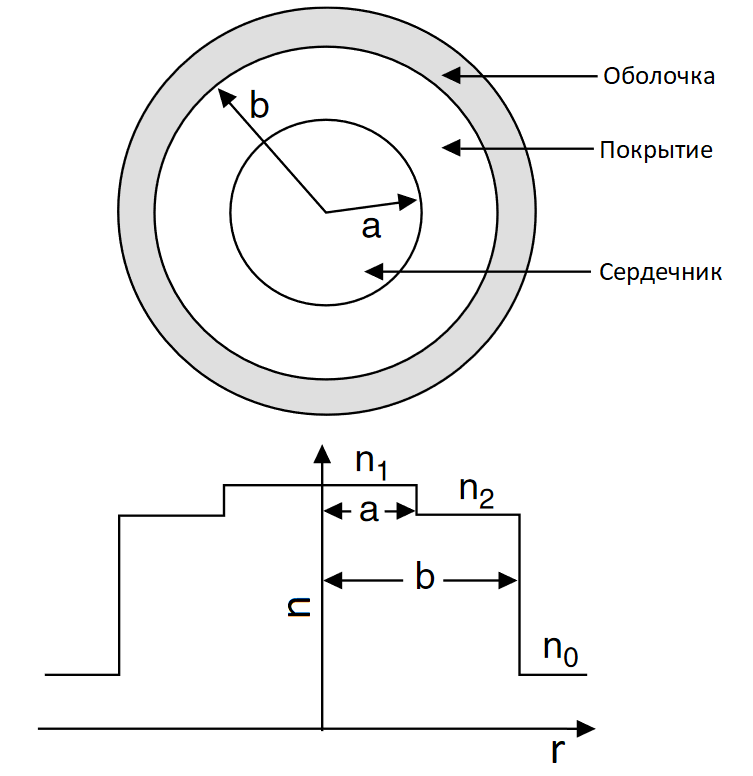
\includegraphics[width=6cm,trim={0 0 0 0},clip]{fig1.png} 
				\caption{Допустимые значения \(M_{1}\) и \(M_{0}.\)}
				\label{fig1}
			\end{figure}

			Волновой профиль (\ref{eq24}) при \(k=1.6,\, M_{0}=-1.48,\, M_{1}=6.16,\,\varepsilon_{2}=2.16,\,\varepsilon_{3}=0.99\) изображён на Рис. \ref{fig8}.
			\begin{figure}[H]
				\center
				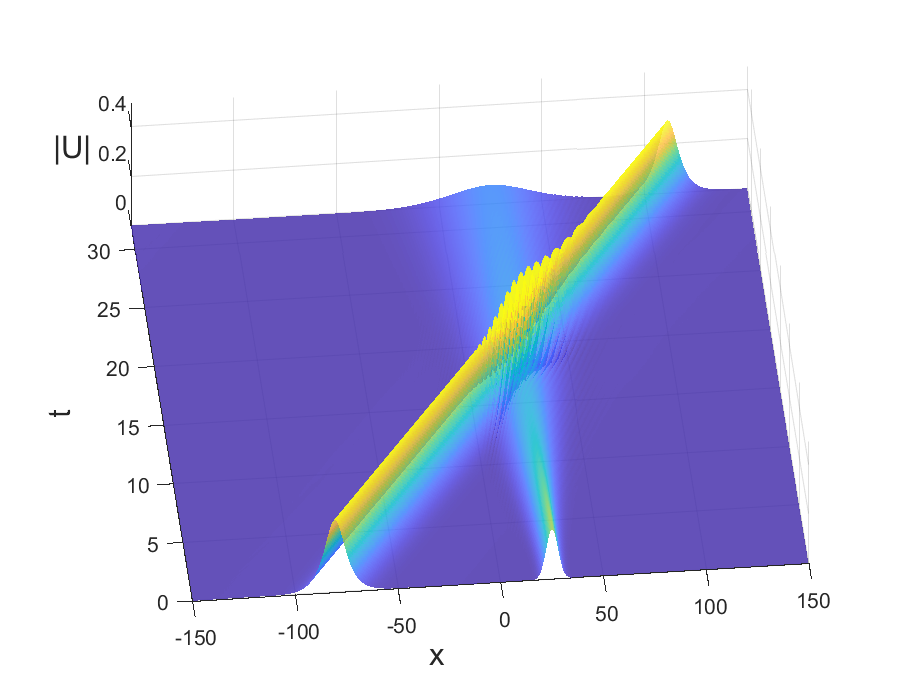
\includegraphics[width=0.5\linewidth]{fig10.eps}
				\caption{Профиль уединённой волны при \(k=1.6,\, M_{0}=-1.48,\, M_{1}=6.16.\)}
				\label{fig8}
			\end{figure}
		\subsection{Модификации численных методов для моделирования процессов, описываемых уравнением Шрёдингера с тремя нелинейностями}\label{ch220}			
			Для численного решения задачи распространения оптических импульсов в рамках изучаемой модели требуется реализовать соответствующую численную схему. Рассмотрим, как это возможно сделать на примере метода расщепления.
			Семейство обобщённых уравнений Шрёдингера может быть записано в виде:
			\begin{equation}\label{eq221}
				u_{t}=i\mathscr{L} [u]+i\mathscr{N}[u]u.
			\end{equation}
			К примеру, при \(\mathscr{L} [u] \equiv a u_{xx},  \,\,  \mathscr{N} [u] \equiv b_{1} |u|^2\) уравнение (\ref{eq221}) представляет из себя нелинейное уравнение Шрёдингера (\ref{eq1}).

			Рассмотрим задачу распространения уединённых импульсов и объявим периодические граничные условия следующим образом:
			\begin{equation} \label{eq30}
				\begin{aligned}
					\begin{cases}
						u\left(-\frac{L}{2},t\right)=u\left(\frac{L}{2},t\right),\\
						\cfrac{\partial u}{\partial x}\left(-\frac{L}{2},t\right)=\cfrac{\partial u}{\partial x}\left(\frac{L}{2},t\right).
					\end{cases}
				\end{aligned}
			\end{equation}

			Предполагая \( x \in [-\frac{1}{2} L, \frac{1}{2} L]\), \( t \in [0, T]\), разделим интервал по переменной \(x\) на \(N\) одинаковых частей с шагом
			\begin{equation}
				h=\frac{L}{N}.
			\end{equation}

			Узлы координатной сетки определяются, как
			\begin{equation}\label{eq220-2}
				x_{j}=jh, \quad j= -\frac{N}{2}, \ldots , \frac{N}{2}.
			\end{equation}

			Пусть \(\boldsymbol{U}^{m}\) - сеточная аппроксимация решения на \(m\)-ном временном слое, и \(\boldsymbol{V}^{m}\) - промежуточное решение. В таком случае, начальные условия задаются в \(\boldsymbol{U}^{0}\). В общем виде, схема расщепления может быть записана следующим образом \cite{Rad1}:
			\begin{equation}\label{eq34}
				\boldsymbol{U}^{m+1}=e^{i\tau\mathscr{L}}\boldsymbol{V}^m,
			\end{equation}
			где
			\begin{equation}\label{eq33}
				\boldsymbol{V}^m=e^{i\tau\mathscr{N}[\boldsymbol{U}^m]}\boldsymbol{U}^m.
			\end{equation}

			В некоторых случаях, явный вид \(\mathscr{N}[u]\), позволяет напрямую вычислить \(\boldsymbol{V}^m\). Например, в случае уравнения (\ref{eq120-1}) выражение (\ref{eq33}) запишется следующим образом:
			\begin{equation}\label{eq222}
				\boldsymbol{V}^m = e^{i\tau|\boldsymbol{U}^m|^2 \left(1 + \varepsilon_{2}|\boldsymbol{U}^m|^2+ \varepsilon_{3}|\boldsymbol{U}^m|^4\right)}\boldsymbol{U}^m
			\end{equation}
			
			В зависимости от метода аппроксимации оператора \(e^{i\tau\mathscr{L}}[u]\) возможно получить различные численные схемы для решения задачи распространения оптических импульсов, основанные на методе расщепления. 
			
			\subsubsection{Конечно-разностный метод}\label{ch221}
				Для получения модификации конечно-разностного метода решения задачи распространения оптических импульсов, используем соотношение:
				\begin{equation}
					e^{i\tau\mathscr{L}}=\left(\mathscr{I}-\theta i\tau\mathscr{L}\right)^{-1}\left(\mathscr{I}+(1-\theta) i\tau\mathscr{L}\right),
				\end{equation}
				где \(\mathscr{I}\) - тождественный оператор, \(\theta\) - параметр в пределах \( 0\le\theta\le1\). При этом выражение (\ref{eq34}) запишется в виде:
				\begin{equation}\label{eq223}
					\left(\mathscr{I}-\theta i\tau\mathscr{L}\right)\boldsymbol{U}^{m+1}=\left(\mathscr{I}+(1-\theta) i\tau\mathscr{L}\right)\boldsymbol{V}^m.
				\end{equation}
				
				Введём разностный оператор:
				\begin{equation}
					\mathscr{L}_{h}\left[\boldsymbol{U}_{j}\right]=\left(\boldsymbol{U}_{j+1}-2\boldsymbol{U}_{j}+\boldsymbol{U}_{j-1}\right)/h^2, \quad j= -\frac{N}{2}, \ldots , \frac{N}{2}-1.
				\end{equation}
				Тогда соотношение (\ref{eq223}) запишется в матричной форме:
				\begin{equation} \label{eq224}
					\left(I-ir\theta S\right)\boldsymbol{U}^{m+1}=\left(I+ir(1-\theta S)\right)\boldsymbol{V}^m,
				\end{equation}
				где \(I\) - тождественная матрица, \( r=\tau/h^2\),
				\begin{equation} 
					\boldsymbol{U}=\left(U_{-N/2},\ldots ,U_{N/2-1}\right)^T,
				\end{equation}
				\begin{equation} 
					S=
					\begin{pNiceMatrix}[r]
					-2& 1& .& .& 1\\
					1& -2& 1& . &.\\
					.& .& .& . &.\\
					.& .& 1& -2& 1\\
					1 &.& . &-2& 1
					\end{pNiceMatrix}.
				\end{equation}

				Соотношения (\ref{eq222}) и (\ref{eq224}) полностью определяют конечно-разностный метод решения задачи распространения оптических импульсов в рамках модели (\ref{eq120-1}).

			\subsubsection{Псевдоспектральный метод Фурье}\label{ch222}
				Альтернативный подход, приводящий к псевдоспектральному методу Фурье - использование дискретного преобразования Фурье для сеточной функции \(\boldsymbol{V}^m\) для определения решения на следующем временном слое:
				\begin{equation} \label{eq222-1}
					\hat{\boldsymbol{V}}^m=\frac{h}{L}\exp\left(-i \boldsymbol{\mu} \boldsymbol{x}^{T}\right)\cdot \boldsymbol{V}^{m},
				\end{equation}
				где \(\hat{\boldsymbol{V}}^m\) - вектор коэффициентов Фурье, \(\boldsymbol{\mu}=\left(\mu_{-N/2},\ldots,\mu_{N/2-1}\right)^{T}\) - вектор частот преобразования \(\mu_{n}=\frac{2\pi n}{L}\), \(\boldsymbol{x}=\left(x_{-N/2},\ldots,x_{N/2-1}\right)^{T}\) - координаты точек сетки.

				Воспользуемся соотношением между \(\hat{\boldsymbol{U}}^{m+1}\) и \(\hat{\boldsymbol{V}}^{m}\),
				\begin{equation} \label{eq46}
					\hat{\boldsymbol{U}}^{m+1}=\exp\left(-i \left(\boldsymbol{\mu}\circ \boldsymbol{\mu}\right) \tau\right)\circ \hat{\boldsymbol{V}}^{m},
				\end{equation}
				которое вытекает из уравнения (\ref{eq34}) после подстановки в него вместо \(\boldsymbol{U}^{m+1}\) и \(\boldsymbol{V}^{m}\) соответствующих рядов Фурье. Под \(x\circ y\) понимается произведение по Адамару.

				Решение на следующем временном слое восстанавливается с помощью обратного преобразования Фурье, используя (\ref{eq46}):
				\begin{equation} \label{eq222-2}
					\boldsymbol{U}^{m+1}=\exp\left(i \boldsymbol{\mu} \boldsymbol{x}^{T}\right)\cdot \hat{\boldsymbol{U}}^{m+1}.
				\end{equation}

				Таким образом, соотношения (\ref{eq222}) и (\ref{eq222-1}-\ref{eq222-2}) полностью определяют псевдоспектральный метод Фурье решения задачи распространения оптических импульсов в рамках модели (\ref{eq120-1}).
	\section{Численный анализ}\label{ch300}
		\subsection{Сравнение и валидация численных методов решения задачи распространения оптических импульсов}\label{ch310}
			Для проверки описанных в разделе \ref{ch220} численных схем проведём их валидацию и сравнение на примере моделирования процессов распространения уединённых волн, описываемых классическим НУШ. Рассмотрим (\ref{eq200-4}) при \(\varepsilon_{2}=0,\,\varepsilon_{3}=0\):
			\begin{equation}\label{e6}
				iu_{t}+u_{xx}+|u|^2 u=0.
			\end{equation}
			Задача Коши для уравнения (\ref{e6}) решается методом обратной задачи рассеяния. Его решение в виде уединенной волны представлено в работе \cite{Rad3} и имеет вид:
			\begin{equation} \label{eq48}
				u(x,t)=\frac{4(k^{2}-\omega)}{2 (k^{2}-\omega) e^{-\left(x-c_{0}t-z_{0}\right)\sqrt{(k^{2}-\omega)}}+e^{\left(x-c_{0}t-z_{0}\right)\sqrt{(k^{2}-\omega)}}}\cdot e^{i(kx-\omega t-\theta_{0})},
			\end{equation}
			где \(c_{0}=2k\) и \( k,\, \omega,\, z_{0},\, \theta_{0}\) - произвольные константы.
			Начальное условие, относящееся к решению (\ref{eq48}) представляется следующим образом:
			\begin{equation}\label{eq55}
				u(x,0)=\frac{4\,(k^{2}-\omega)}{2 (k^{2}-\omega) e^{-(x-z_{0})\sqrt{(k^{2}-\omega)}}+e^{(x-z_{0})\sqrt{(k^{2}-\omega)}}}\cdot e^{i(kx-\theta_{0})}
			\end{equation}
			В качестве метрики на пространстве численных и соответствующих им аналитических решений на \(n\) временном слое будем использовать следующую величину:
			\begin{equation}\label{eq300-1}
				\Delta_{\%}^{n}=\frac{\displaystyle\mathop{\max}_{1 \leq m \leq N_{x}}\left(\Big|\big|U^{m,n}_{true}\big|-\big|U^{m,n}\big|\Big|\right)}{\displaystyle\mathop{\max}_{1 \leq m \leq N_{x}}\big|U^{m,n}_{true}\big|} \cdot 100\%,
			\end{equation}
			где \(N_{x}=N+1\) - количество x-узлов сетки на каждом временном слое согласно (\ref{eq220-2}), \(U^{m,n}\) - численное решение, \(U^{m,n}_{true}\) - сеточная редукция соответствующего аналитического решения. В качестве метрики для всего расчёта будем принимать максимальную из ошибок на временных слоях:
			\begin{equation}\label{eq300-1}
				\Delta_{\%}=\max_{1 \leq n \leq N_{t}}\Delta_{\%}^{n}.
			\end{equation}
			Данные величины представляют из себя относительные ошибки в процентах. Отношение берётся к характерной амплитуде импульса.
			Результаты моделирования процесса распространения уединённой волны (\ref{eq48}) при помощи двух описанных в разделе \ref{ch220} методов представлены на Рис. \ref{fig300-1}.
			\begin{figure}[H]
				\center
				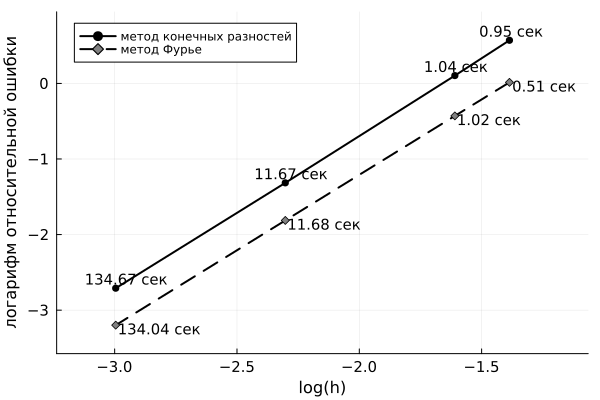
\includegraphics[width=10cm,trim={0 0 0 0},clip]{pic2.png}
				\caption{Зависимости логарифма относительной ошибки от логарифма шага \(h\) по координате \(x\) при моделировании процесса распространения волны (\ref{eq48}) с использованием конечно-разностного и Фурье методов с затраченным на расчёт временем при параметрах
				\(k=0.15,\,\omega=0.4,\,\theta_{0}=0,\,z_{0}=0,\,L=160,\, T=25, \, h=[0.25, 0.2, 0.1, 0.05],\, \tau=h^{2}.\)}
				\label{fig300-1}
			\end{figure}

			Решения, полученные двумя схемами согласуются с аналитическим решением (\ref{eq48}). Сеточная сходимость достигнута. Обе схемы имеют второй порядок аппроксимации по координате и первый порядок аппроксимации по времени. С точки зрения вычислительной сложности и эффективности обе схемы показали схожие результаты. Однако из-за меньшей относительной ошибки в дальнейшей работе будут приводится результаты, полученные псевдоспектральной схемой Фурье.
		\subsection{Применение метода Фурье для моделирования процесса распространения уединённой волны, описываемой уравнением Шрёдингера с тремя нелинейностями}\label{ch320}
			Рассмотрим обобщённое уравнение (\ref{eq200-4}). Смоделируем распространение уединённой волны (\ref{eq24}), полученной в разделе \ref{ch210}. Произведём расчёт для определённых параметров \(M_{0}\) и \(M_{1}\), удовлетворяющих условиям (\ref{eq27}). Параметры \(\varepsilon_{2}\),\,\(\varepsilon_{3}\),\,\(\omega\) и \(\mu\) определяются формулами (\ref{eq19}). Результат моделирования представлен на Рис.\ref{fig10}. Аналитический и численно полученный профили в момент \(t=16\) изображены на Рис. \ref{fig10a}.

			\begin{figure}[H]
				\begin{center}
					\begin{minipage}[h]{0.48\linewidth} %% color here
						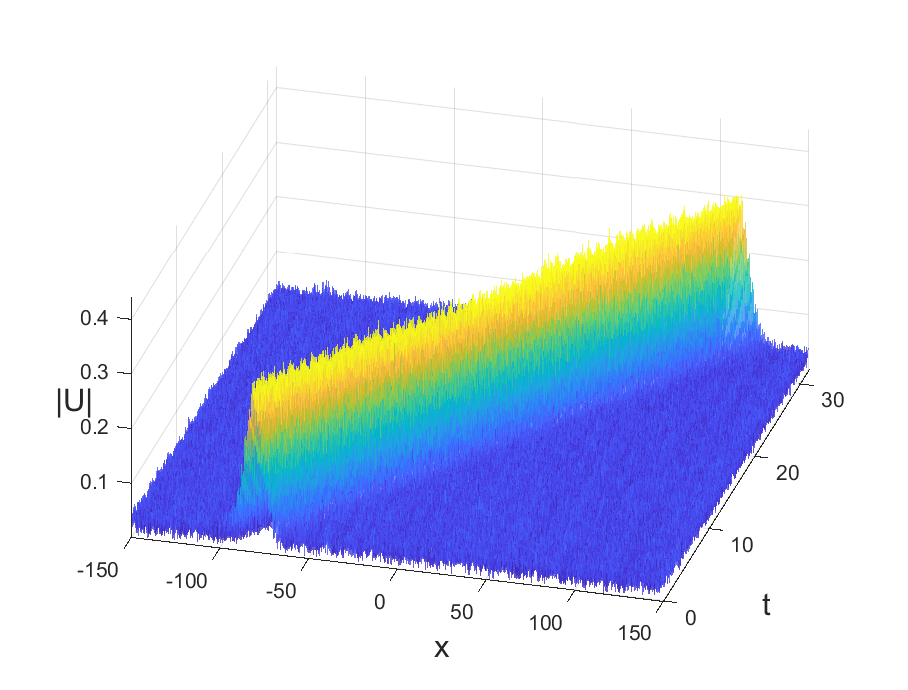
\includegraphics[width=1\linewidth]{fig11.eps}
						\subcaption{Модуль численного решения} 
						\label{fig10a}
					\end{minipage}
					\hfill
					\begin{minipage}[h]{0.48\linewidth}
						\raisebox{-6cm}{
							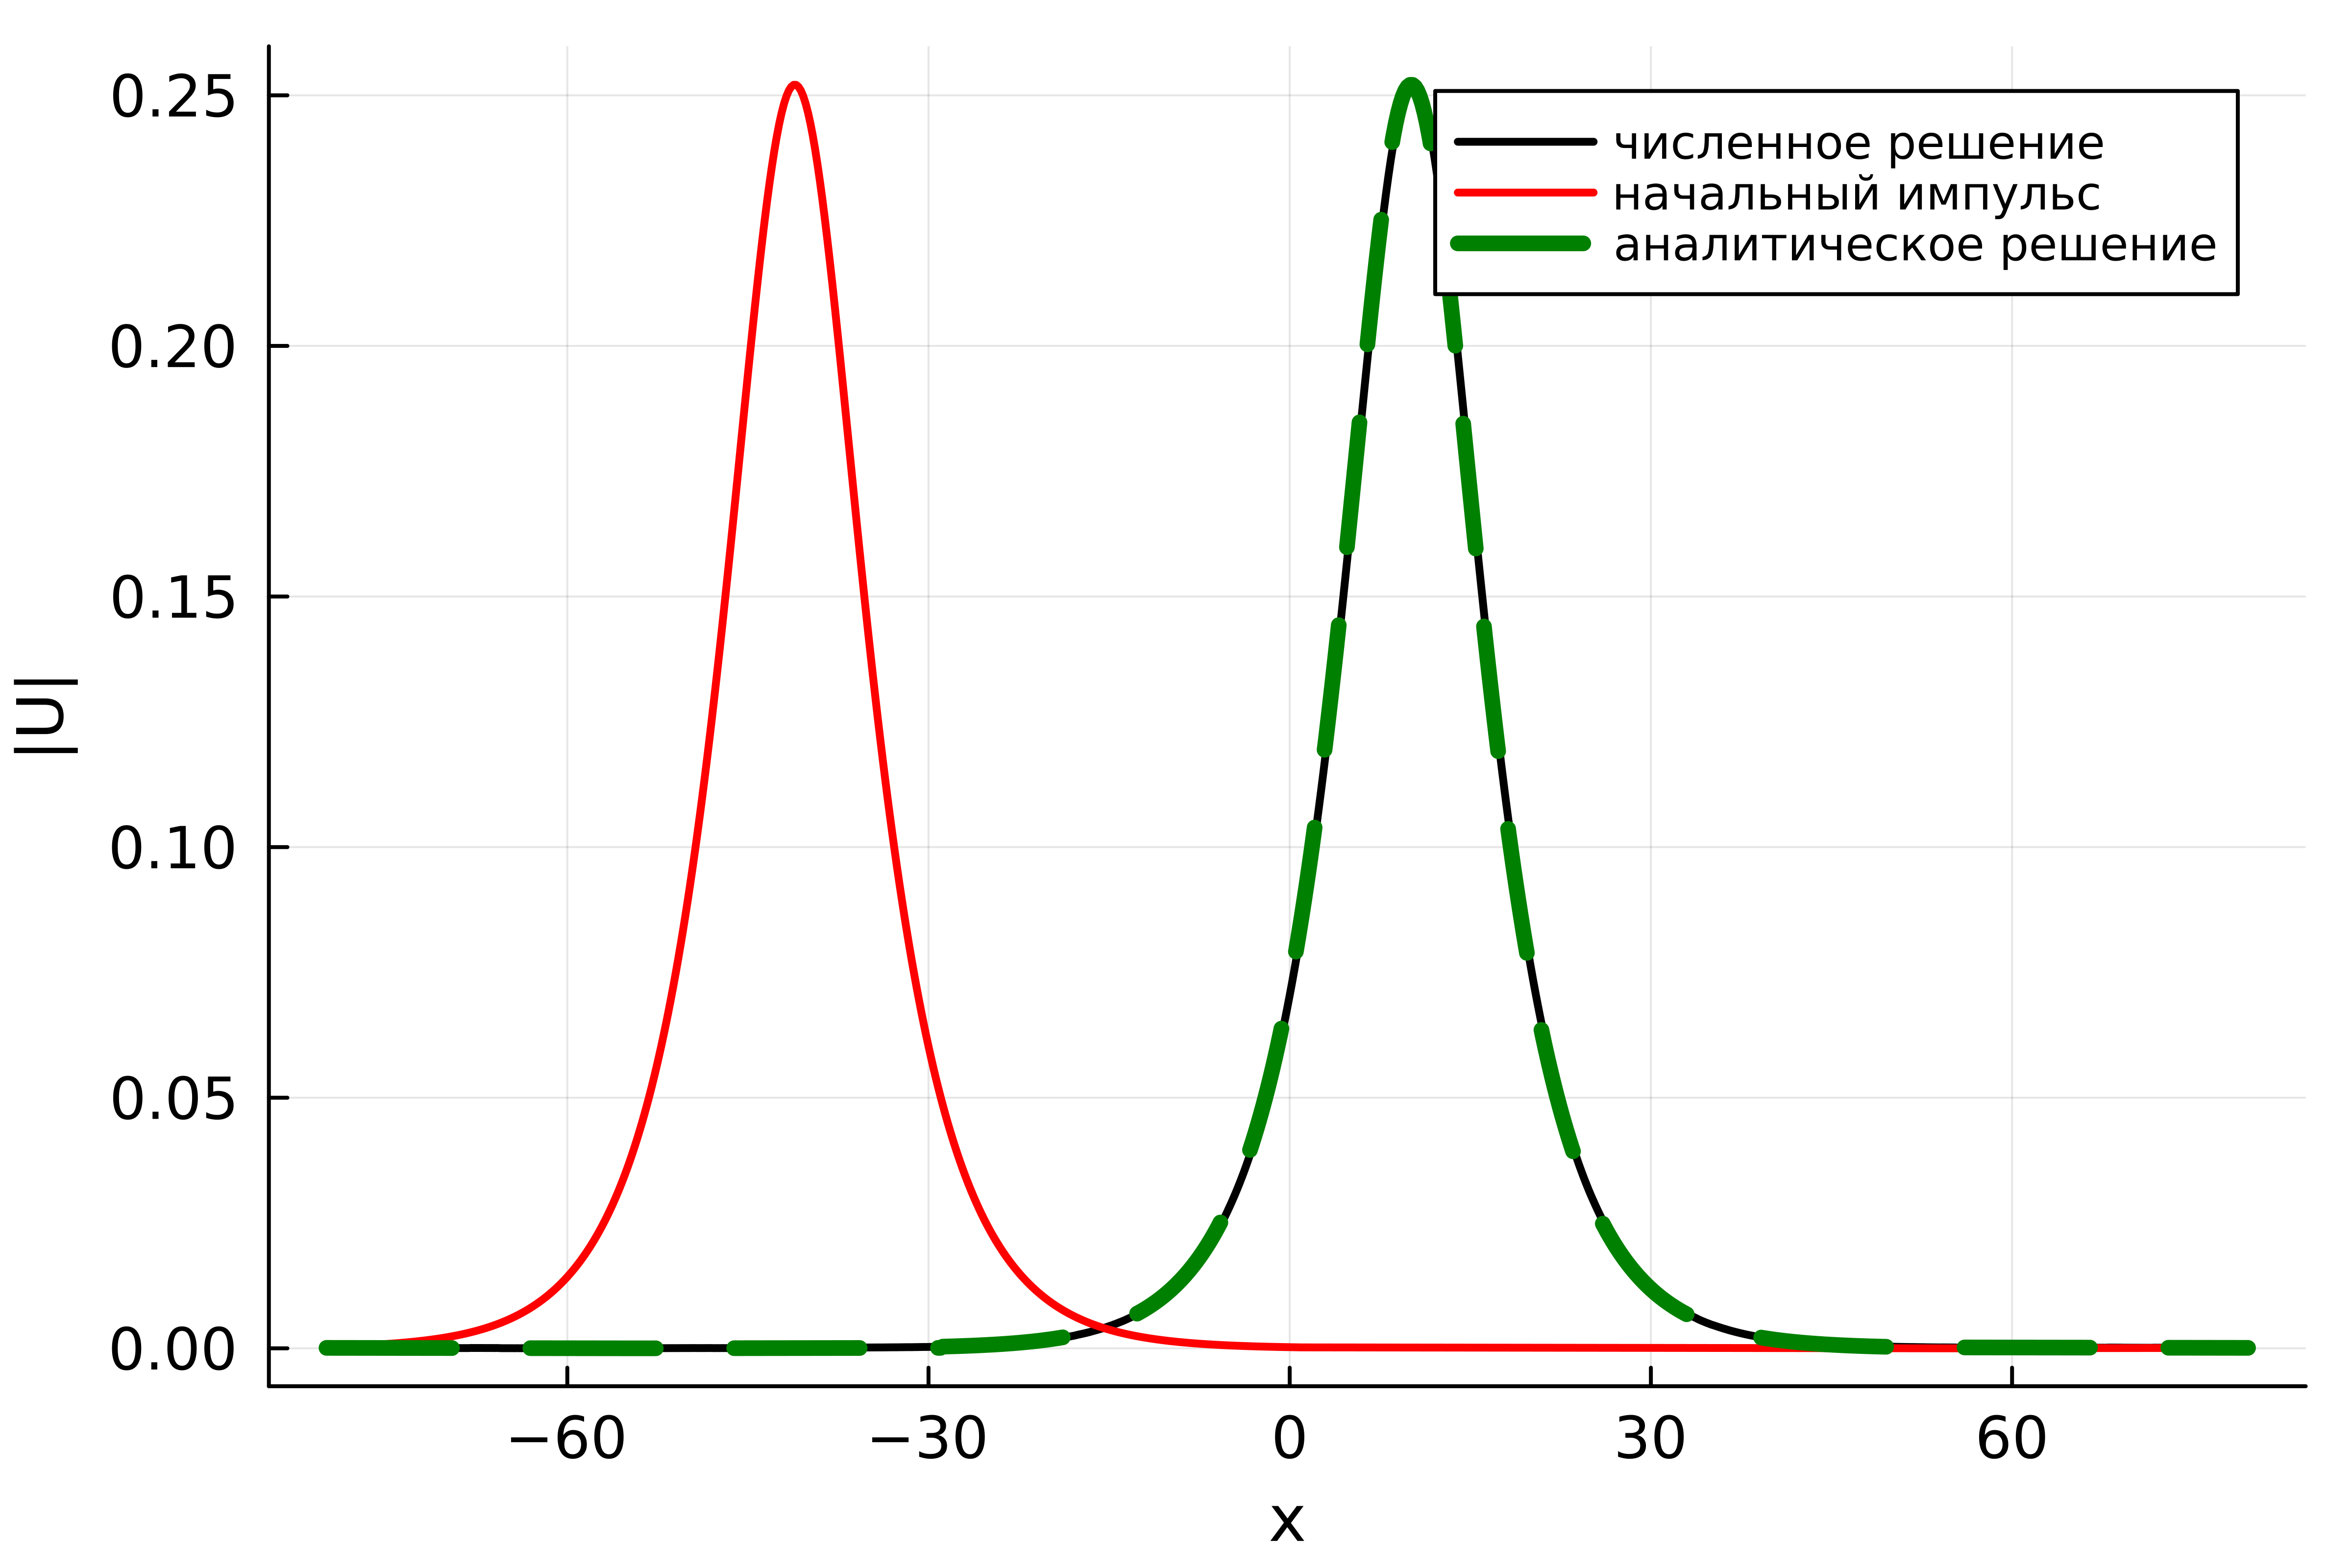
\includegraphics[width=1\linewidth, trim={0 4 0 0},clip]{Medvedev_fig6.png}
						}
						\subcaption{Модули решений при t=16}
						\label{fig10b}
					\end{minipage}
				\end{center}
				\caption{Распространение уединённой волны (\ref{eq24}) \\
				при параметрах
				\(L=120,\, T=16,\, h=0.2,\, \tau=0.04\), 
				\(z_{0}=-20,\,k=1.6,\, M_{0}=-1.48,\, M_{1}=6.16,\,\varepsilon_{2}=2.16,\,\varepsilon_{3}=0.99\).}
				\label{fig10}
			\end{figure}
			Относительная погрешность расчета \(\Delta_{\%}\) при заданных параметрах не превышает 0.1.\%. Зависимость относительной погрешности \(\Delta_{\%}^{n}\) от времени \(t=\tau n\) проиллюстрирована на Рис. \ref{fig11a}.

			\begin{figure}[H]
				\begin{center}
					\begin{minipage}[h]{0.48\linewidth} %% color here
						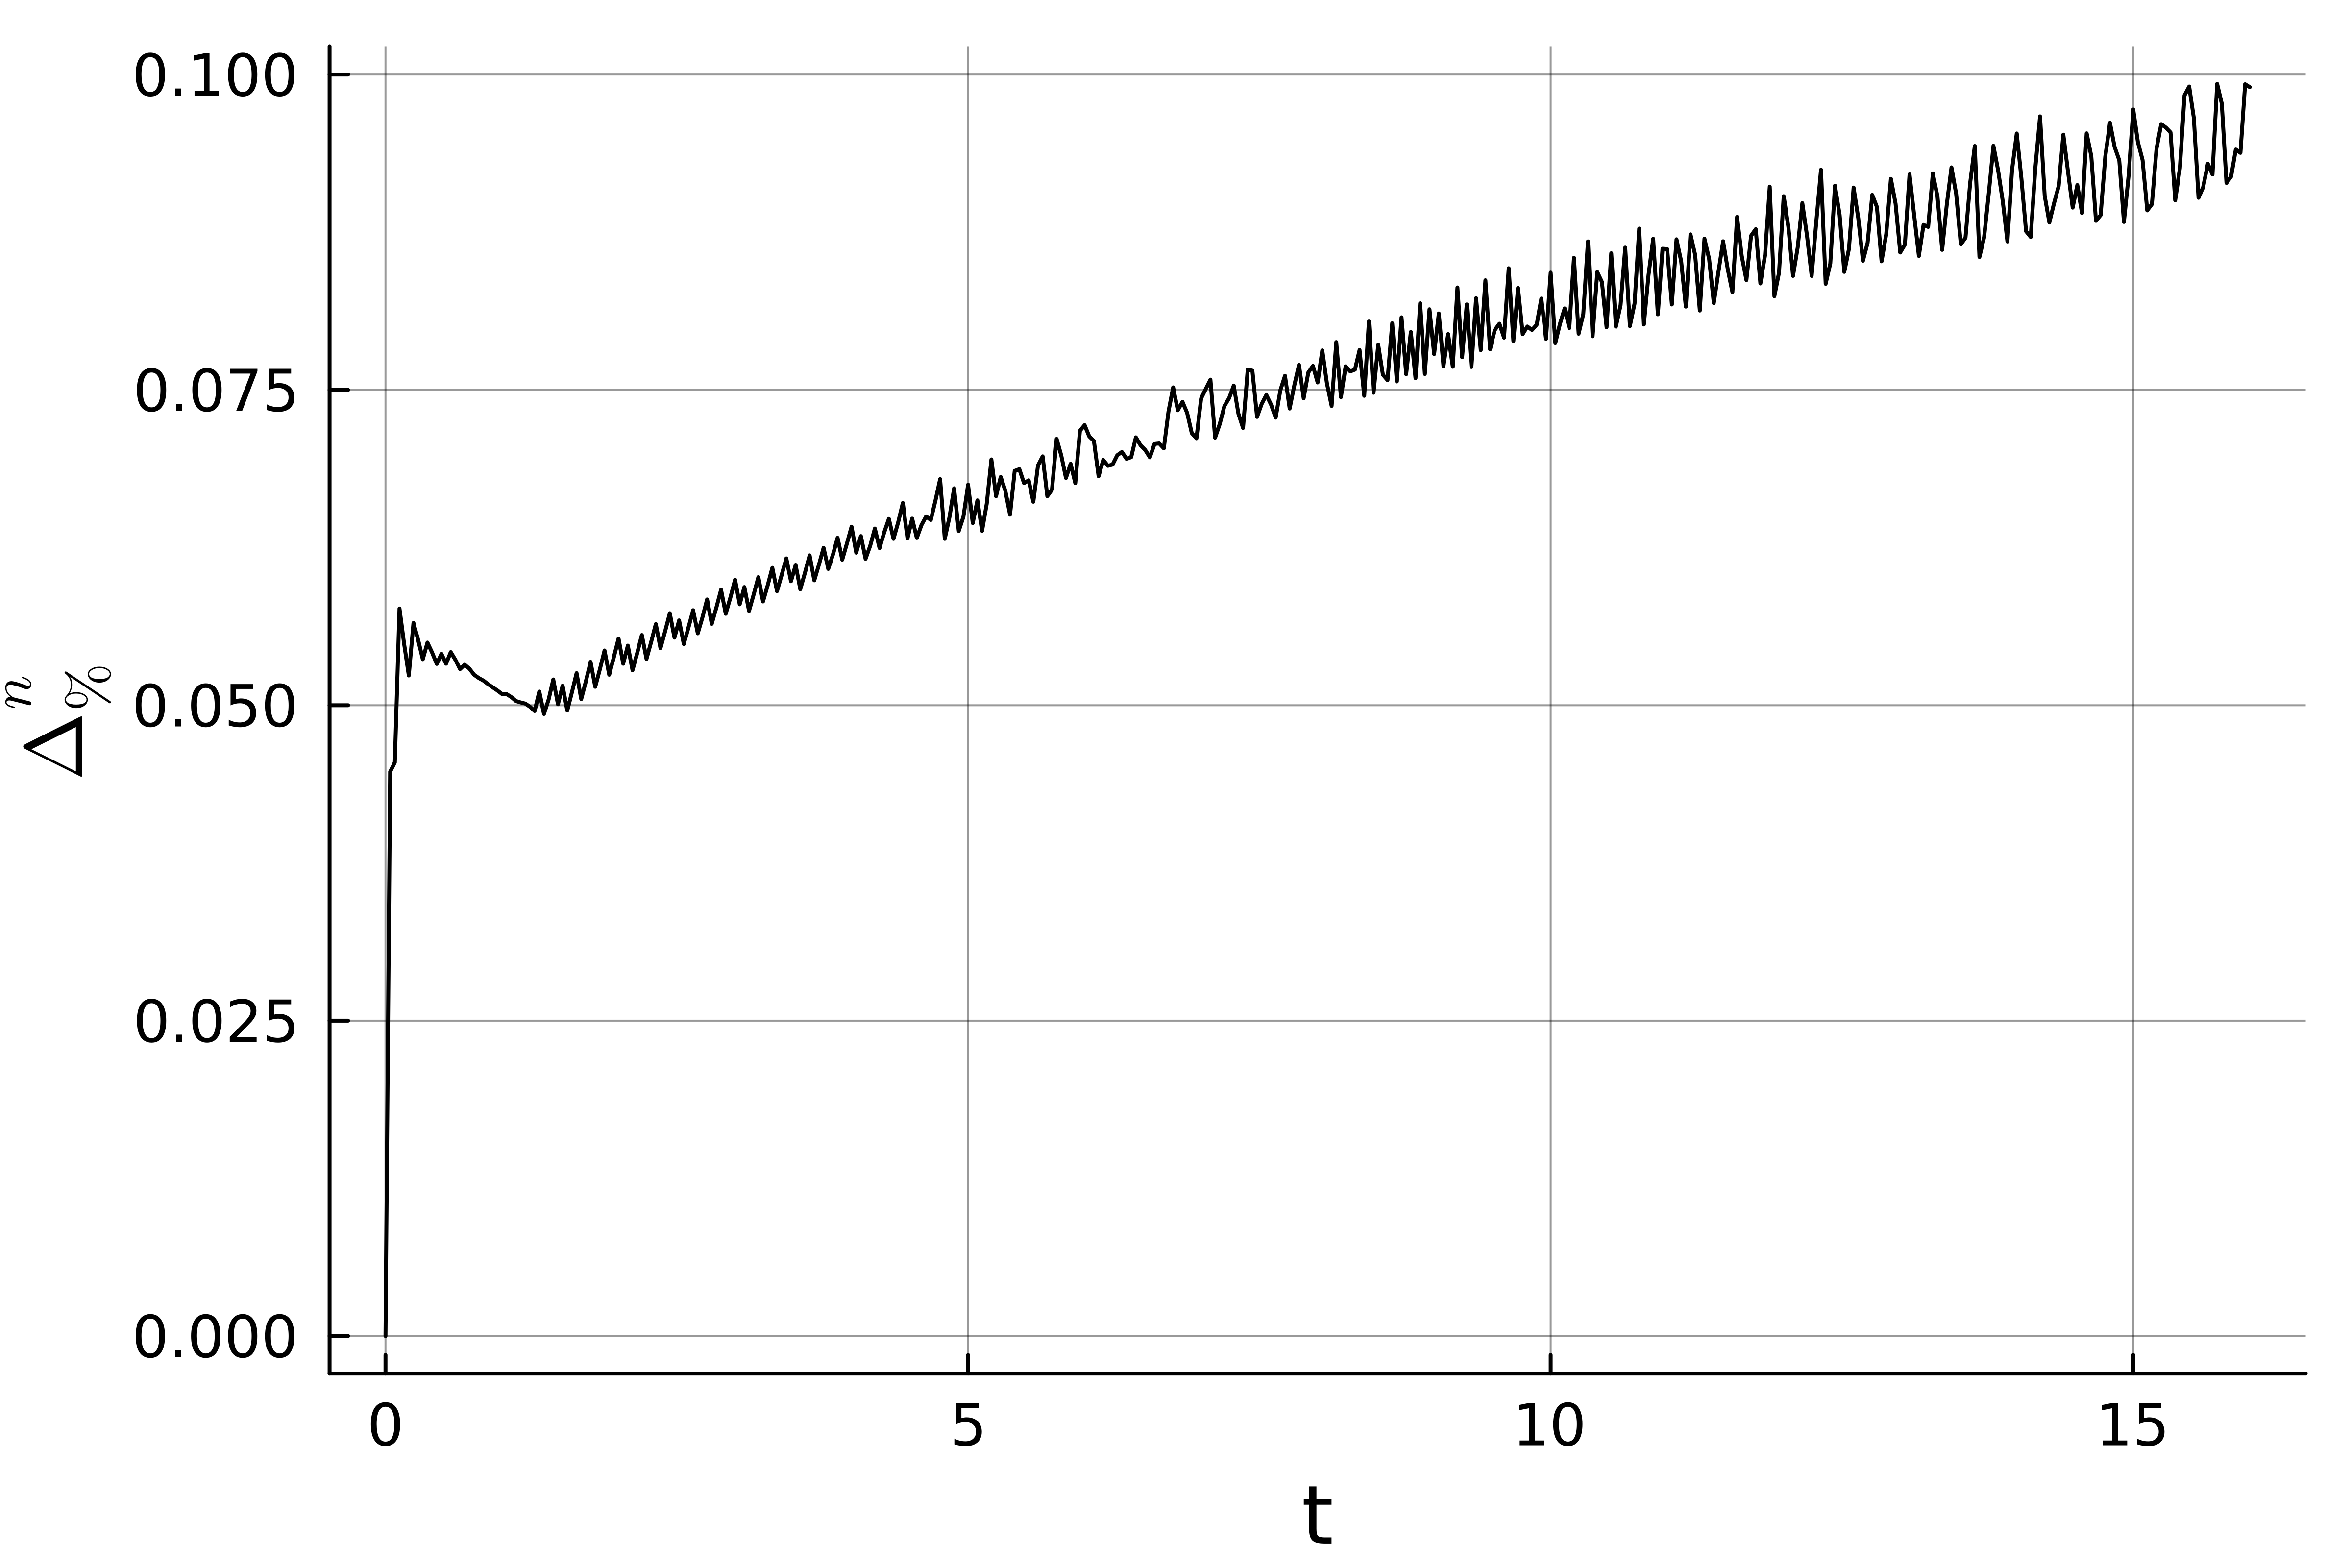
\includegraphics[width=1\linewidth]{Medvedev_fig7.png}
						\subcaption{Относительная ошибка от времени при \(h=0.2,\, \tau=0.04\)} 
						\label{fig11a}
					\end{minipage}
					\hfill
					\begin{minipage}[h]{0.48\linewidth}
						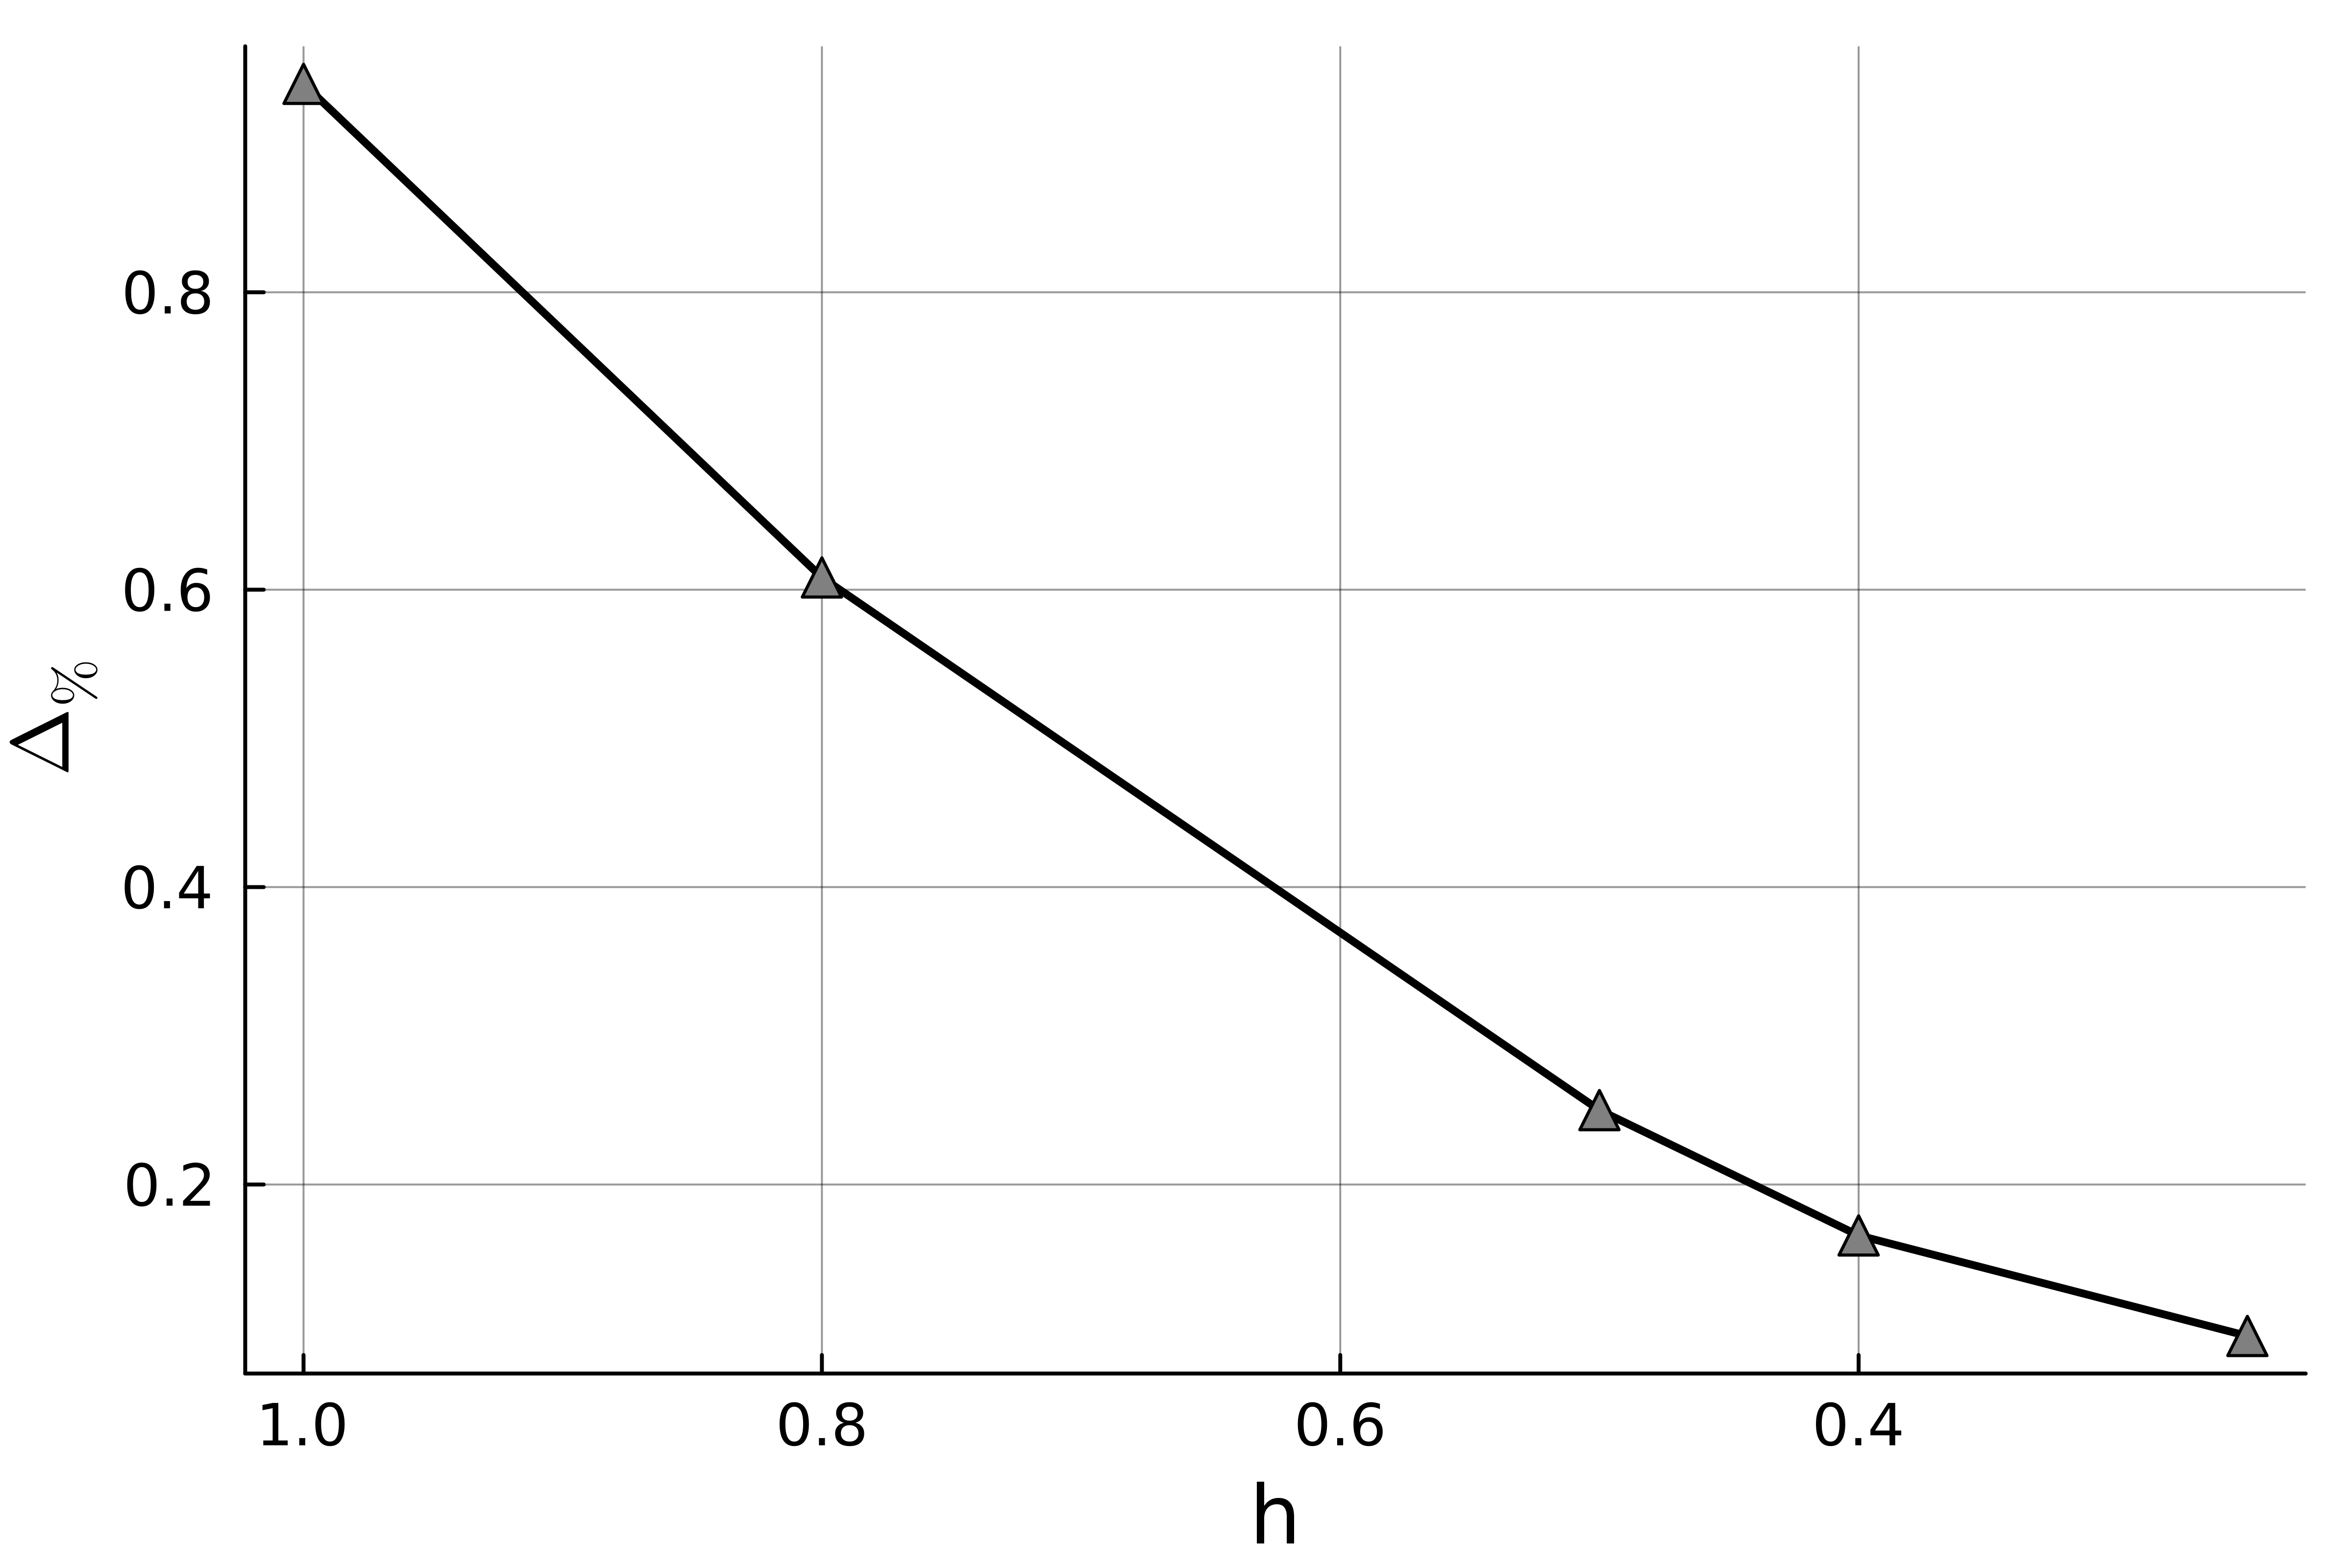
\includegraphics[width=1\linewidth]{Medvedev_fig15.png}
						\subcaption{Максимальная относительная ошибка от шага сетки \(h\)}
						\label{fig11b}
					\end{minipage}
				\end{center}
				\caption{Численные результаты при параметрах
				\(L=160,\, T=16\), 
				\(M_{0}=-1.48,\, M_{1}=6.16,\,\varepsilon_{2}=2.16,\,\varepsilon_{3}=0.99\).}
				\label{fig11}
			\end{figure}
			Сеточная сходимость достигнута (Рис. \ref{fig11b}), аналитическое решение совпало с численным. Следовательно, численная схема корректно описывает процесс распространения оптического импульса для обобщённого уравнения, и есть основание утверждать, что аналитическое решение, построенное в разделе \ref{ch210}, обладает солитонными свойствами.
		\subsection{Взаимодействие солитона с возмущением в начальных условиях}\label{ch330}
			В рамках исследования устойчивости аналитического решения (\ref{eq24}) проведём моделирование распространения импульса при возмущении в начальных условиях. Внесём в начальное условие возмущение следующим образом:
			\begin{equation} \label{eq52}
				u(x,0)=y\left(\xi\left(x\right)\right)\cdot e^{i(kx-\theta_{0})}+Ae^{-\nu(x-x_{0})^{2}},
			\end{equation}
			где \(A\) - амплитуда возмущения. Проведём моделирование для приведённого начального условия.
			Соответствующие численные результаты изображены на Рис. \ref{fig17}.
			\begin{figure}[H] %% color here
				\begin{center}
					\begin{minipage}[h]{0.48\linewidth}
						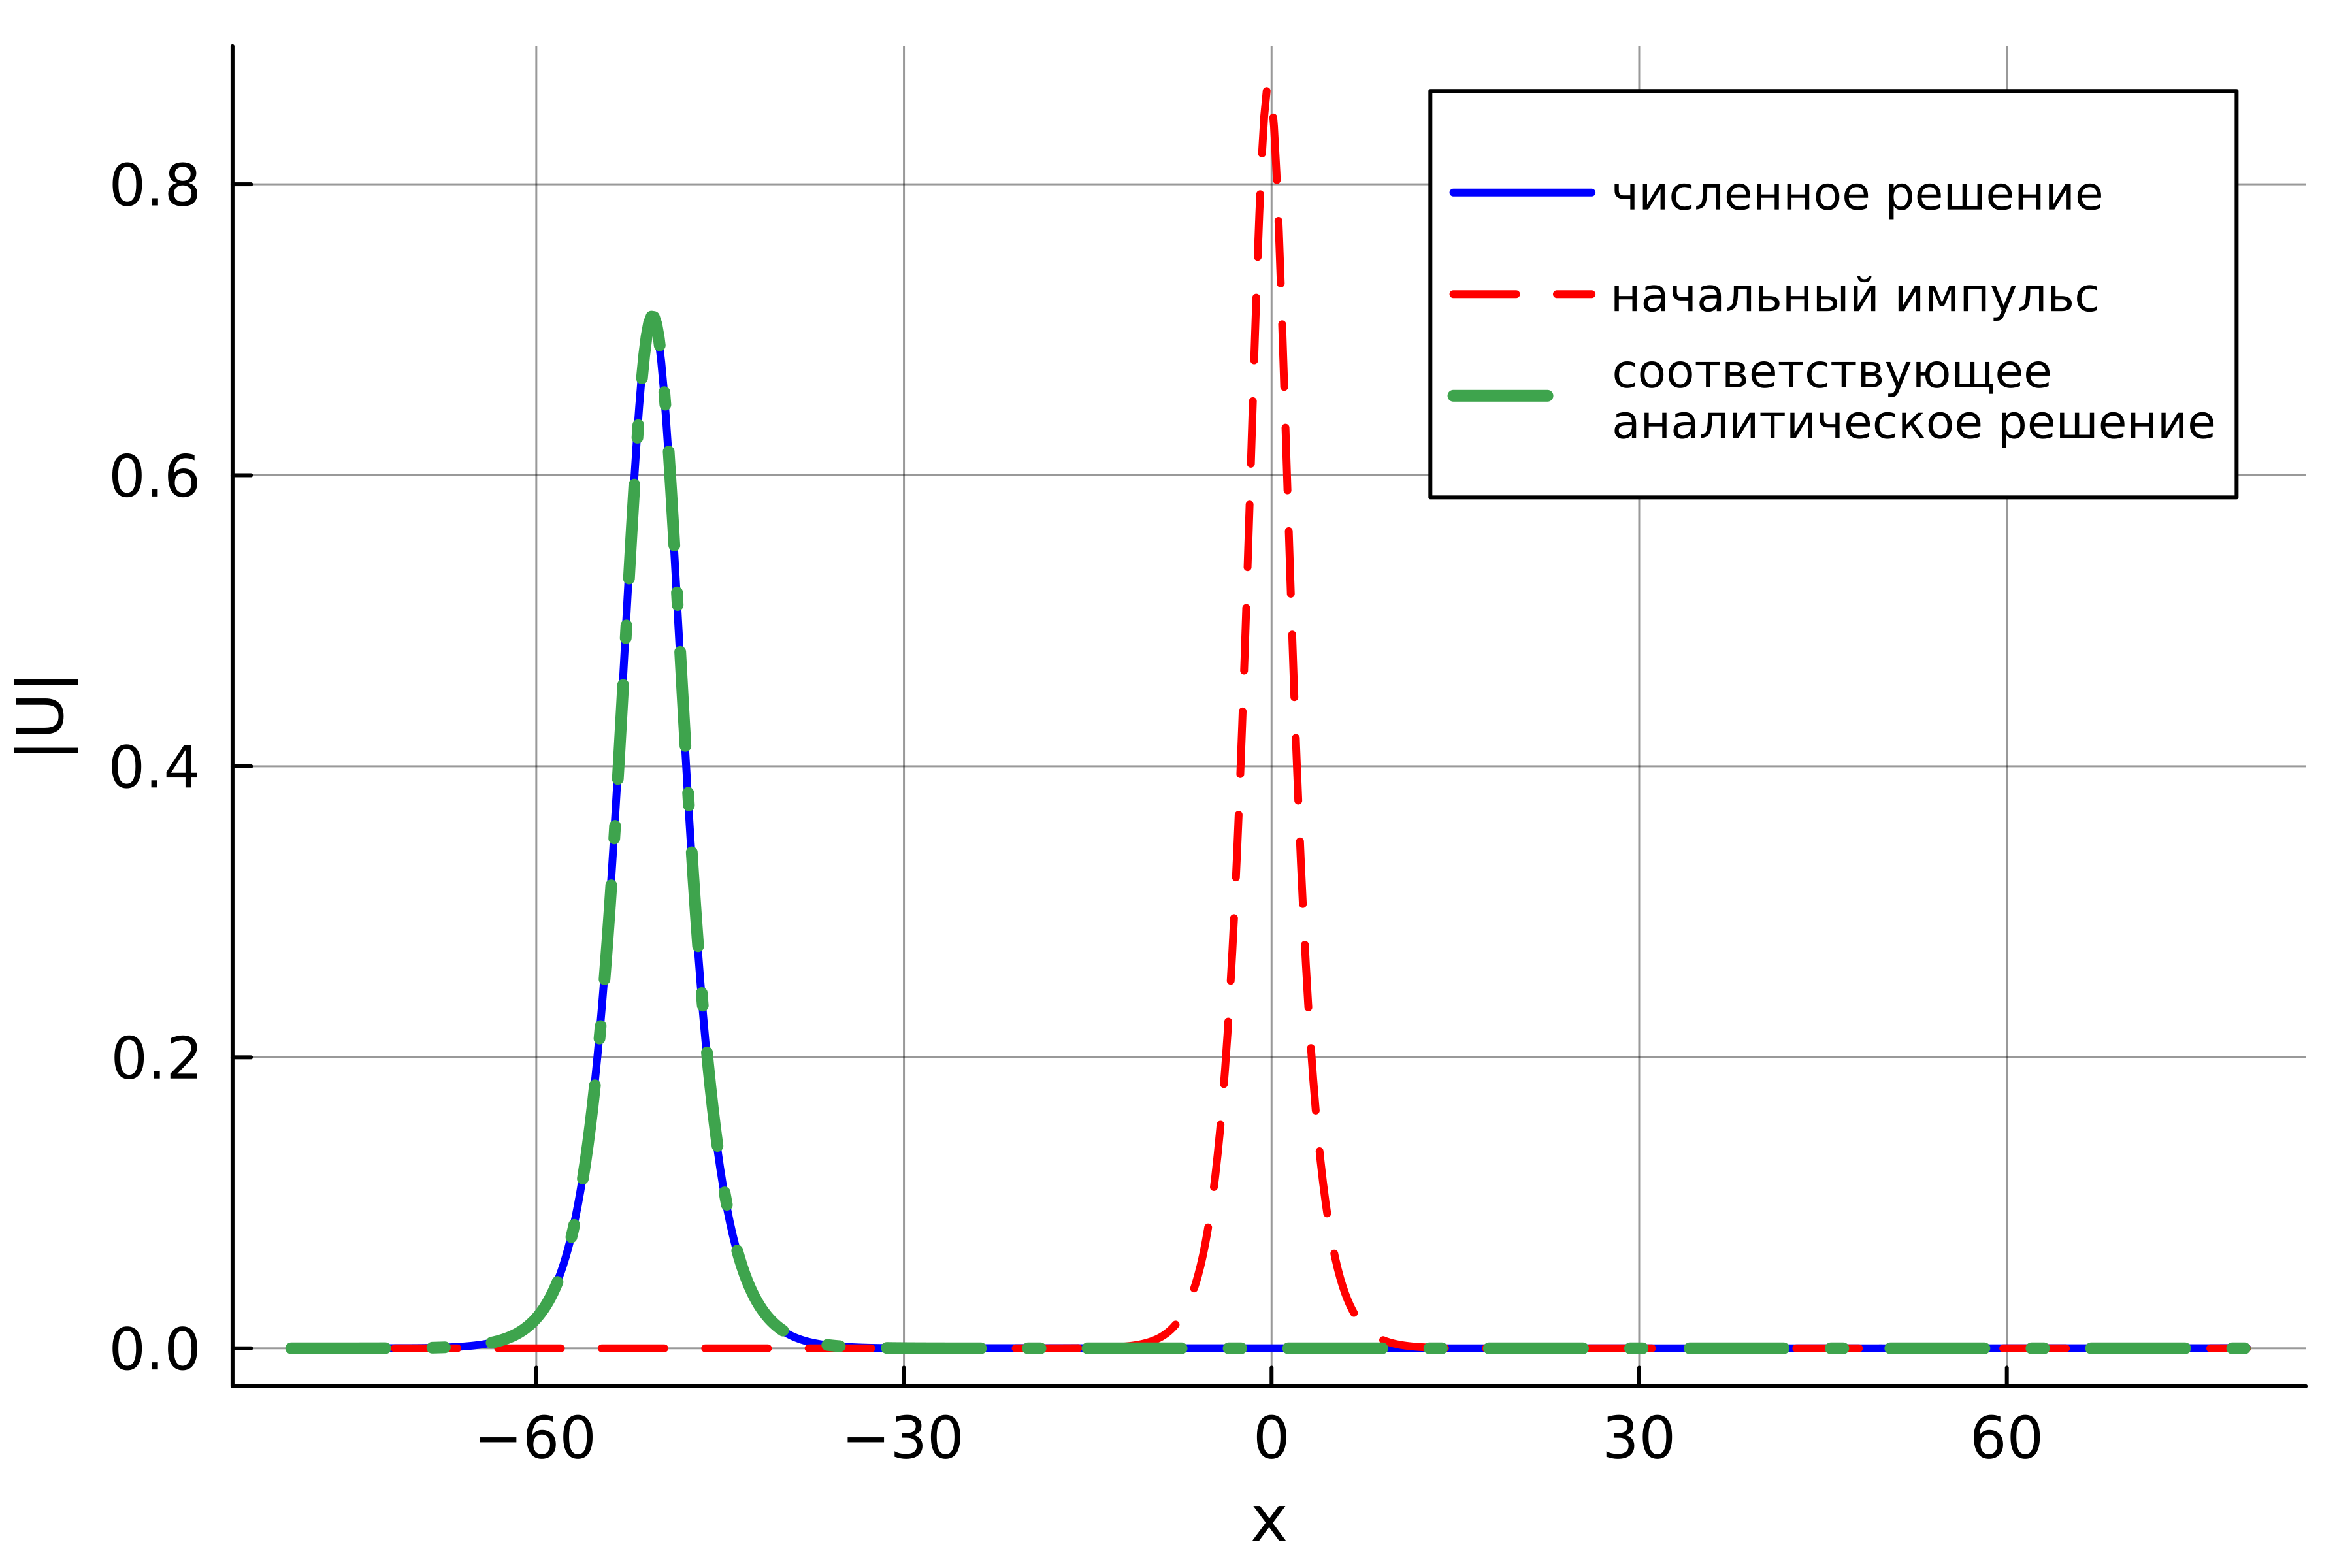
\includegraphics[width=1\linewidth]{fig18.eps}
						\subcaption{Модуль начального условия (\ref{eq52}) }
					\end{minipage}
					\hfill
					\begin{minipage}[h]{0.48\linewidth}
						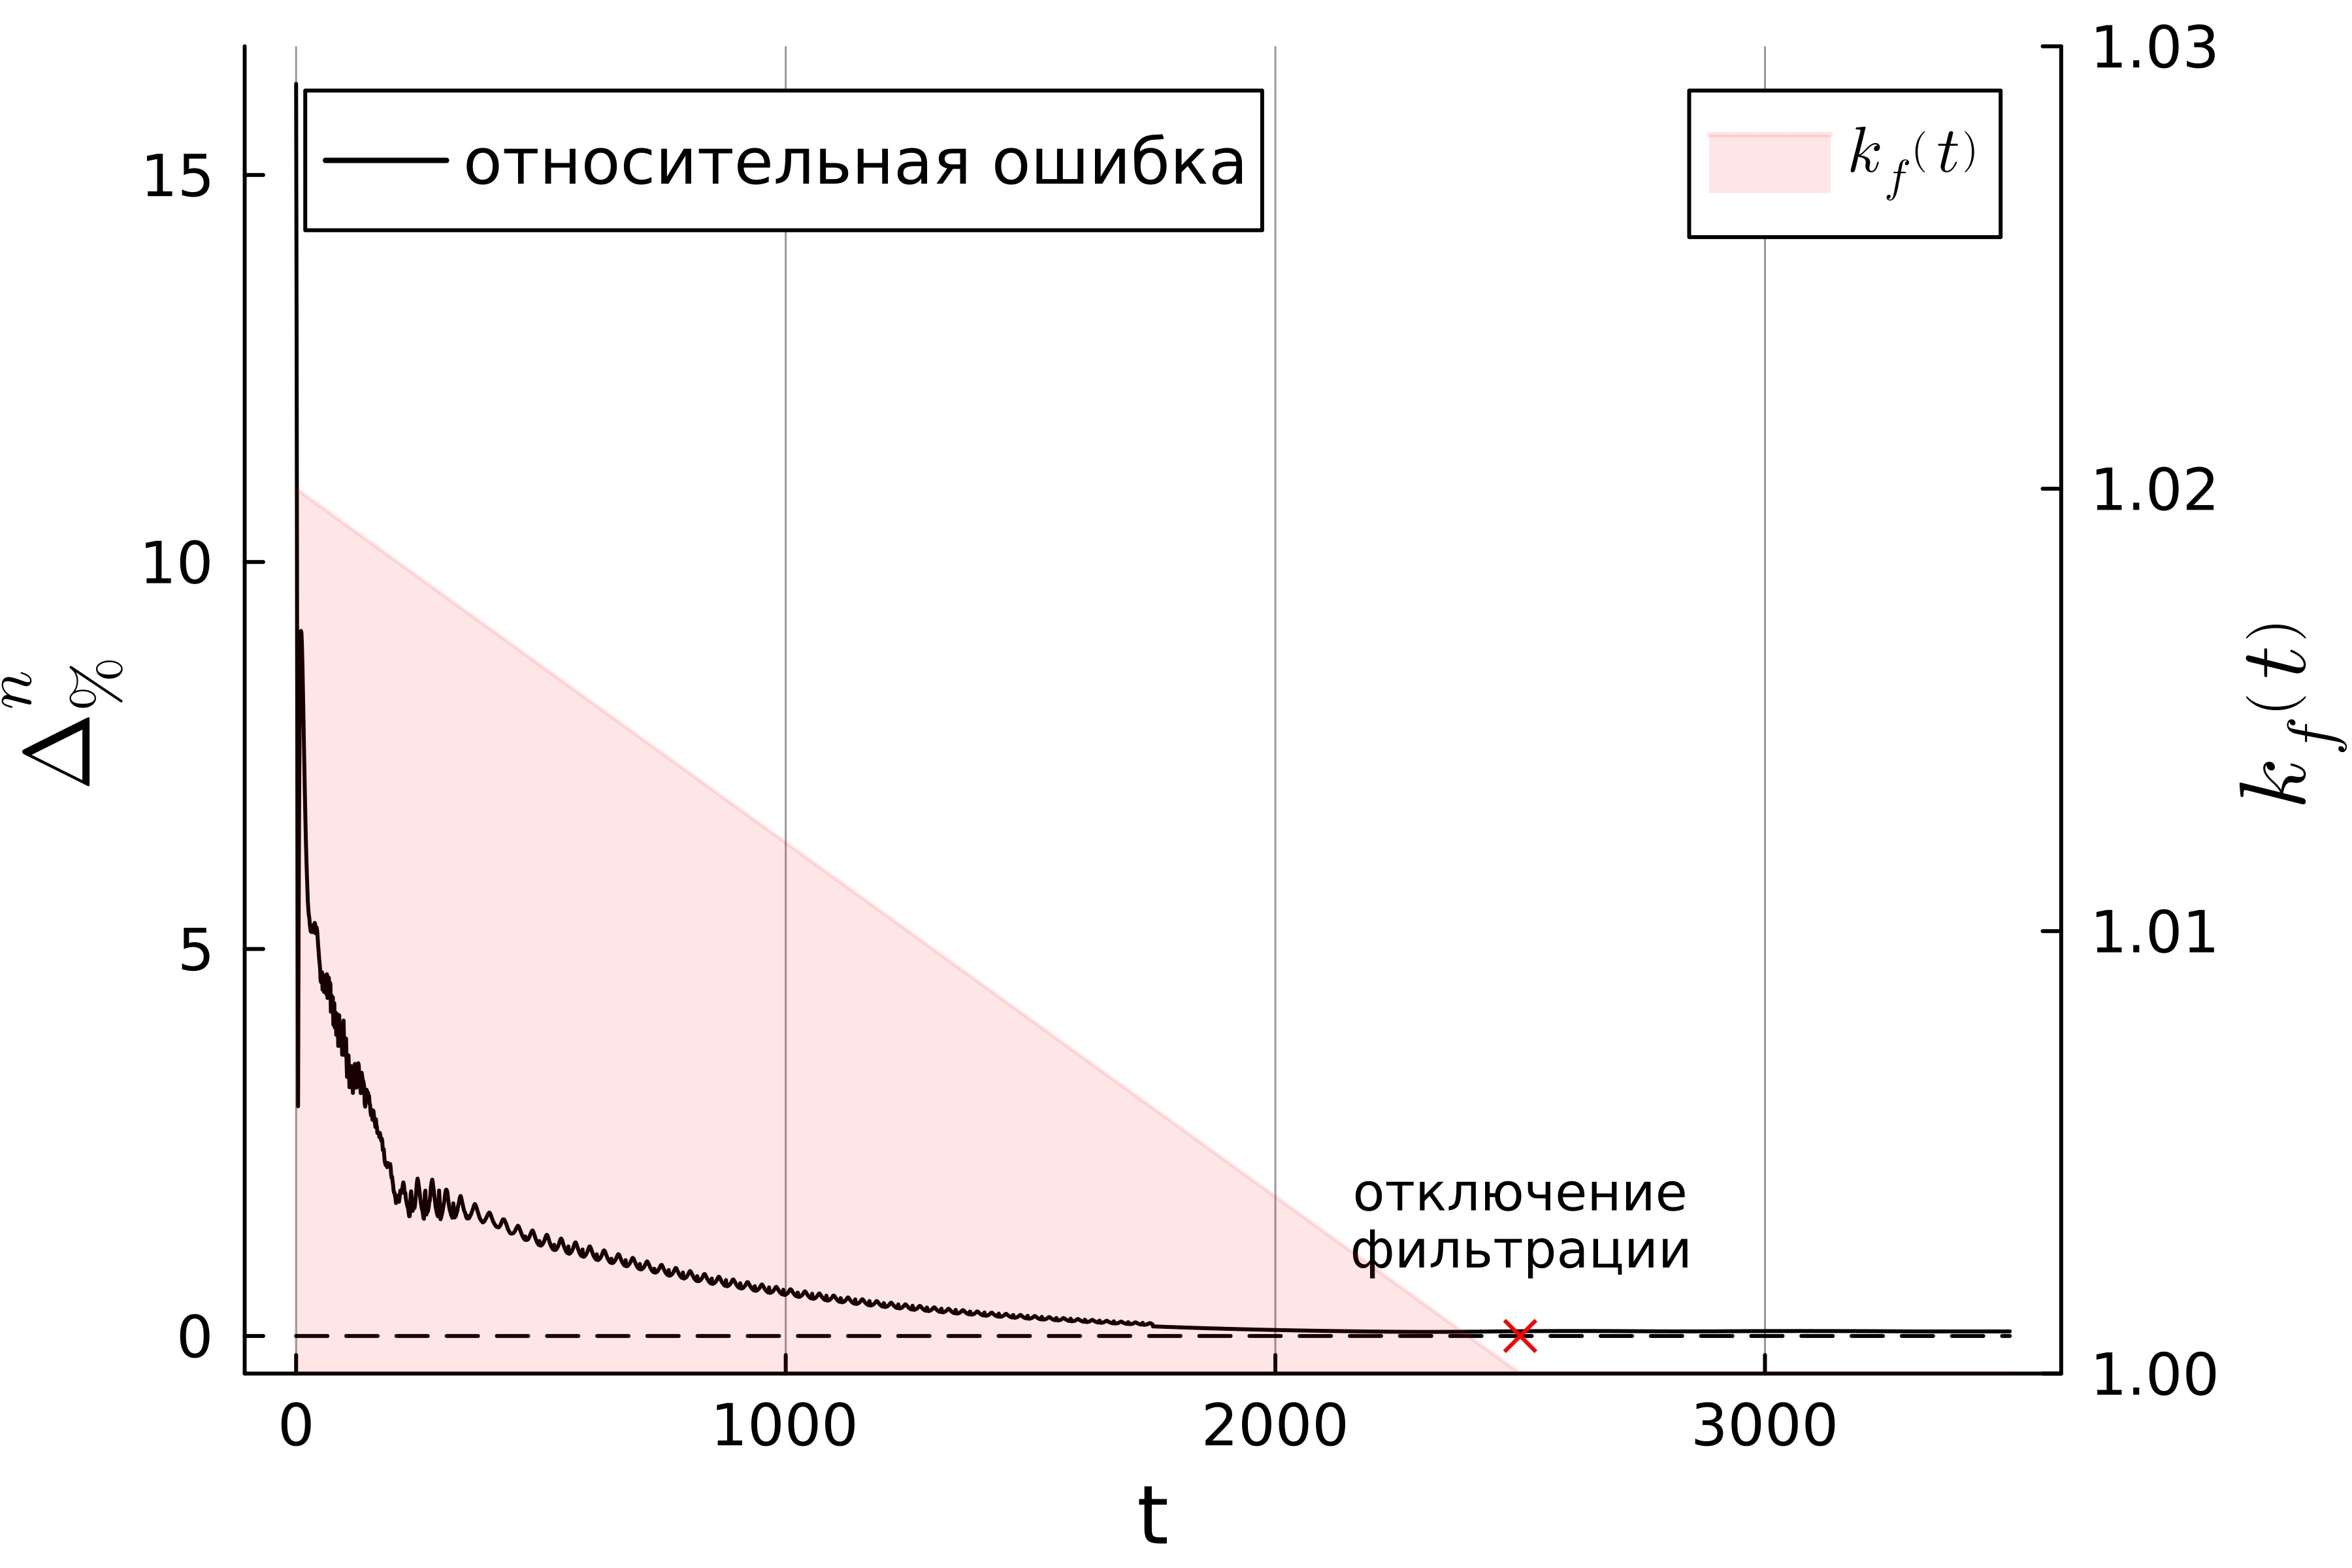
\includegraphics[width=1\linewidth]{fig19.eps}
						\subcaption{Модуль численного решения}
					\end{minipage}
				\end{center}
				\caption{Численные результаты при параметрах \(M_{0}=-3,\,M_{1}=12.34,\,\varepsilon_{2}=1.04,\,\varepsilon_{3}=0.23,\, k=3,\, \xi_{0}=0,\,z_{0}=-80,\, \theta_{0}=0,\, L=300,\, T=32,\, h=0.25,\, \tau=0.625,\,A=0.2,\,\nu=0.06,\, x_{0}=25\).}
				\label{fig17}
			\end{figure}
			Проведённое моделирование позволяет сделать вывод, что солитон, заданный рассмотренными параметрами, взаимодействует с заданным возмущением, не распадаясь и не теряя способности к распространению. Профиль пульса восстанавливается после взаимодействия.

			Также установлено, что солитон уравнения (\ref{eq200-4}) устойчив при распространении в среде со случайным шумом следующего вида:
			\begin{equation} \label{eq522}
				u(x,0)=y\left(\xi\left(x\right)\right)\cdot e^{i(kx-\theta_{0})}+A\cdot rand(x).
			\end{equation}
			Результаты моделирования проиллюстрированы на Рис. \ref{fig172}.	
			\begin{figure}[H] %% color here
				\begin{center}
					\begin{minipage}[h]{0.48\linewidth}
						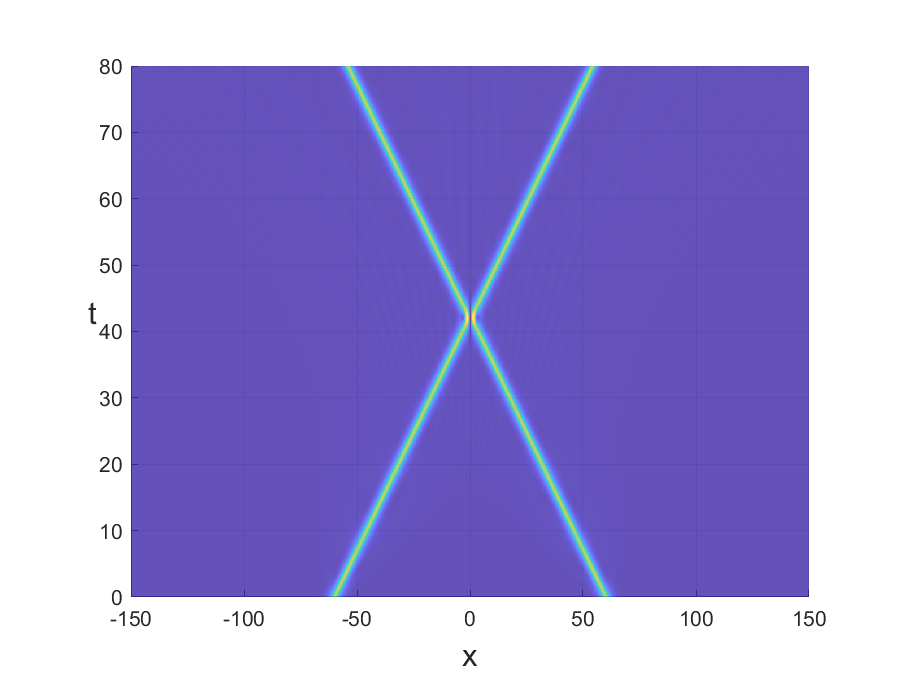
\includegraphics[width=1\linewidth]{fig46.eps}
						\subcaption{Модуль численного решения}
					\end{minipage}
					\hfill
					\begin{minipage}[h]{0.48\linewidth}
						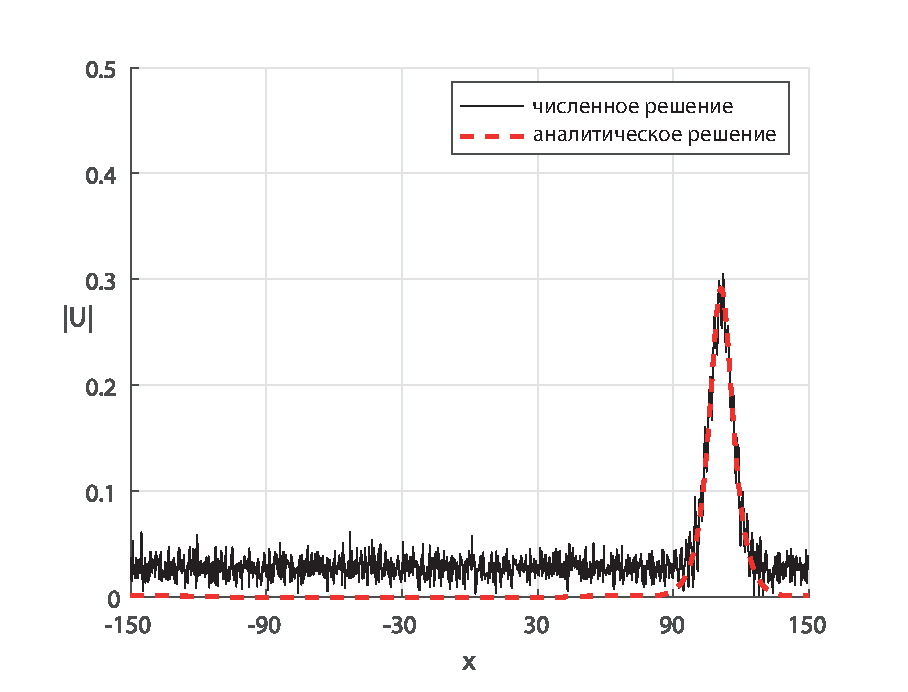
\includegraphics[width=1\linewidth]{Medvedev_fig17.eps}
						\subcaption{Профили решений при t=32}
					\end{minipage}
				\end{center}
				\caption{Численные результаты при параметрах \(M_{0}=-3,\,M_{1}=12.34,\,\varepsilon_{2}=1.04,\,\varepsilon_{3}=0.23,\, k=3,\, \xi_{0}=0,\,z_{0}=-80,\, \theta_{0}=0,\, L=300,\, T=32,\, h=0.25,\, \tau=0.0625,\,A=0.05\).}
				\label{fig172}
			\end{figure}

			Моделирования, представленные в данном разделе, подтверждают стабильность солитонов, полученных в разделе \ref{ch210}.
		\subsection{Анализ влияния высших степеней нелинейности на распространение уединённой волны}\label{ch340}
			При решении физических задач классическое НУШ обобщается путём добавления в уравнение некоторых выражений, учитывающих определённые физические факторы. Поскольку реальные физические процессы могут протекать по более сложным законам, не всегда возможно заранее предугадать и учесть все необходимые уточняющие члены. В этом разделе мы исследуем влияние дополнительных нелинейных членов на решения НУШ. 
			
			Для изучения обсуждаемого влияния приведём несколько полезных уточнений.
			Решение уравнения (\ref{eq200-4}) при \(\varepsilon_{3}=0\) ранее уже было найдено в следующем виде:
			\begin{equation}\label{e7}
				u(x,t)=\left(\frac{4\,\mu\, e^{\sqrt{\mu}\,(x-2kt-z_{0})}}{1+4\, e^{\sqrt{\mu}\,(x-2kt-z_{0})}+(4+4\, \mu\, \nu) \,e^{2\sqrt{\mu}\,(x-2kt-z_{0})}}\right)^{\frac{1}{2}}\cdot e^{i(kx-\omega t-\theta_{0})},
			\end{equation}
			где \(\mu=4(\omega-k^{2})\), \(\nu=\cfrac{4 \varepsilon_{2}}{3}\) и \( k,\, \omega,\, z_{0},\, \theta_{0}\) - произвольные константы. Заметим, что при \(\varepsilon_{2}=0\) решение (\ref{e7}) совпадает с решением (\ref{eq48}).

			Для полноты численного анализа процессов распространения будем проверять выполнение законов сохранения для уравнения (\ref{eq200-4}) в процессе моделирования. Повторяя алгоритм поиска из работы \cite{KudrNifHierarchy}, первые два закона сохранения для мощности и переносимого импульса можно записать в следующем виде:
			\begin{equation}\label{eq320-2}
				I_{1}=\int\limits_{-\infty}^{\infty} |u|^{2} \, dx,
			\end{equation}
			\begin{equation}\label{eq320-3}
				I_{2}=-i \int\limits_{-\infty}^{\infty}\left(u^{*}u_{x}-u u^{*}_{x}\right) dx.
			\end{equation}

			Для сеточной функции численного решения на временном слое \(n\) воспользуемся следующими выражениями для аппроксимации значений интегралов (\ref{eq320-2}) и (\ref{eq320-3}):
			\begin{equation}\label{eq320-4}
				I_{1,n}^{(h)}=\sum_{1 \leq m \leq N_{x}} |U^{m,n}|^{2} \, dx,
			\end{equation}
			\begin{equation}\label{eq320-5}
				I_{2,n}^{(h)}=-i \sum_{1 \leq m \leq N_{x}}\left(\big(U^{m,n}\big)^{*}\dot{U}^{m,n}-U^{m,n} \big(\dot{U}^{m,n}\big)^{*}\right) dx,
			\end{equation}
			где \(\dot{U}\) - узловая аппроксимация производной. Для этого будем использовать трехузловые формулы численного дифференцирования со вторым порядком аппроксимации:
			\begin{equation}\label{eq320-6}
				\begin{aligned}	
					&\dot{U}_{0} = \frac{-3U_{0} + 4U_{1} - U_{2}}{2h},\\
					&\dot{U}_{m} = \frac{U_{m+1} - U_{m-1}}{2h},\\
					&\dot{U}_{N_{x}} = \frac{U_{N_{x}-2} - 4U_{N_{x}-1} + 3U_{N_{x}}}{2h}.
				\end{aligned}
			\end{equation}

			Исследуем влияние нелинейных выражений на распространение уединённой волны нелинейного уравнения Шрёдингера (\ref{eq48}) в рамках обобщённой нелинейной модели, описываемой уравнением (\ref{eq200-4}).

			При \(\varepsilon_{2}=0,\,\varepsilon_{3}=0\) уединенная волна (\ref{eq48}) является точным решением уравнения (\ref{eq200-4}). Численное решение для начального условия (\ref{eq55}) совпадает с аналитическим. Поведение законов сохранения (\ref{eq320-2}) и (\ref{eq320-3}) проиллюстрировано на рисунке \ref{fig340-1}, где \(\delta\) - относительная точность сохранения величины соответствующего интеграла.
			\begin{figure}[H] %% color here
				\begin{center}
					\begin{minipage}[h]{0.48\linewidth}
						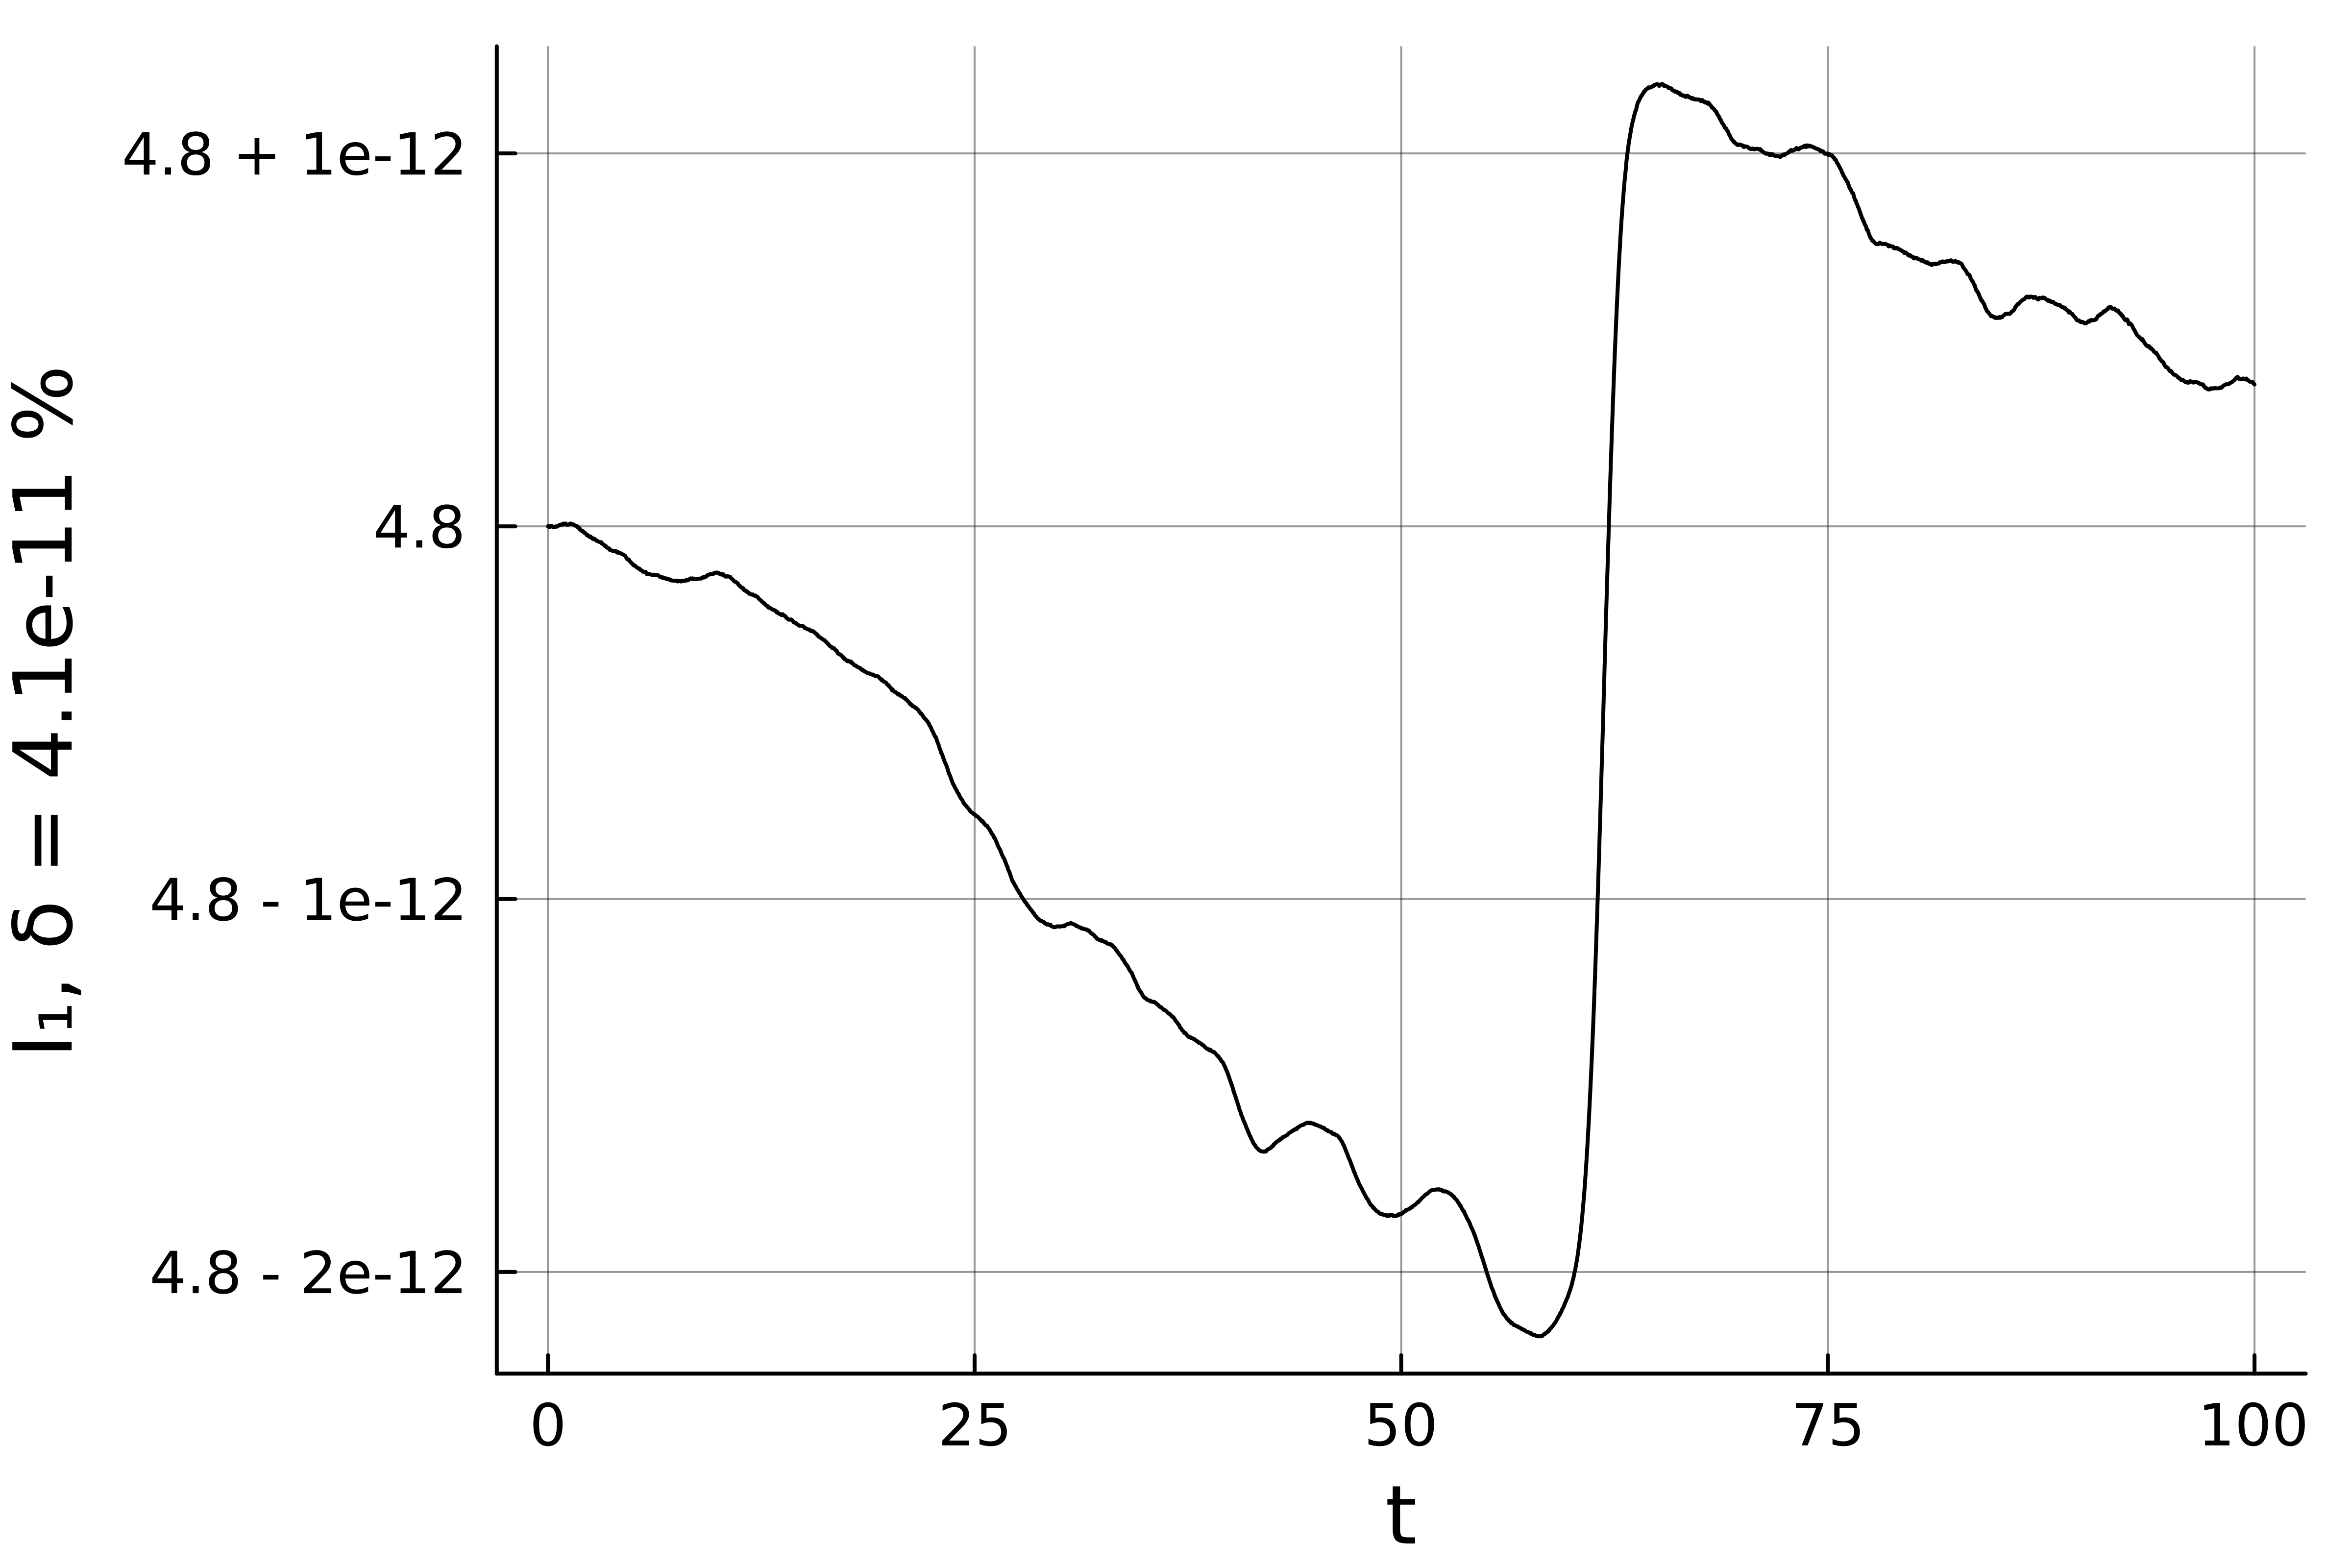
\includegraphics[width=1\linewidth]{fig61.png}
						\subcaption{Зависимость \(I_{1}\) от времени.}
					\end{minipage}
					\hfill
					\begin{minipage}[h]{0.48\linewidth}
						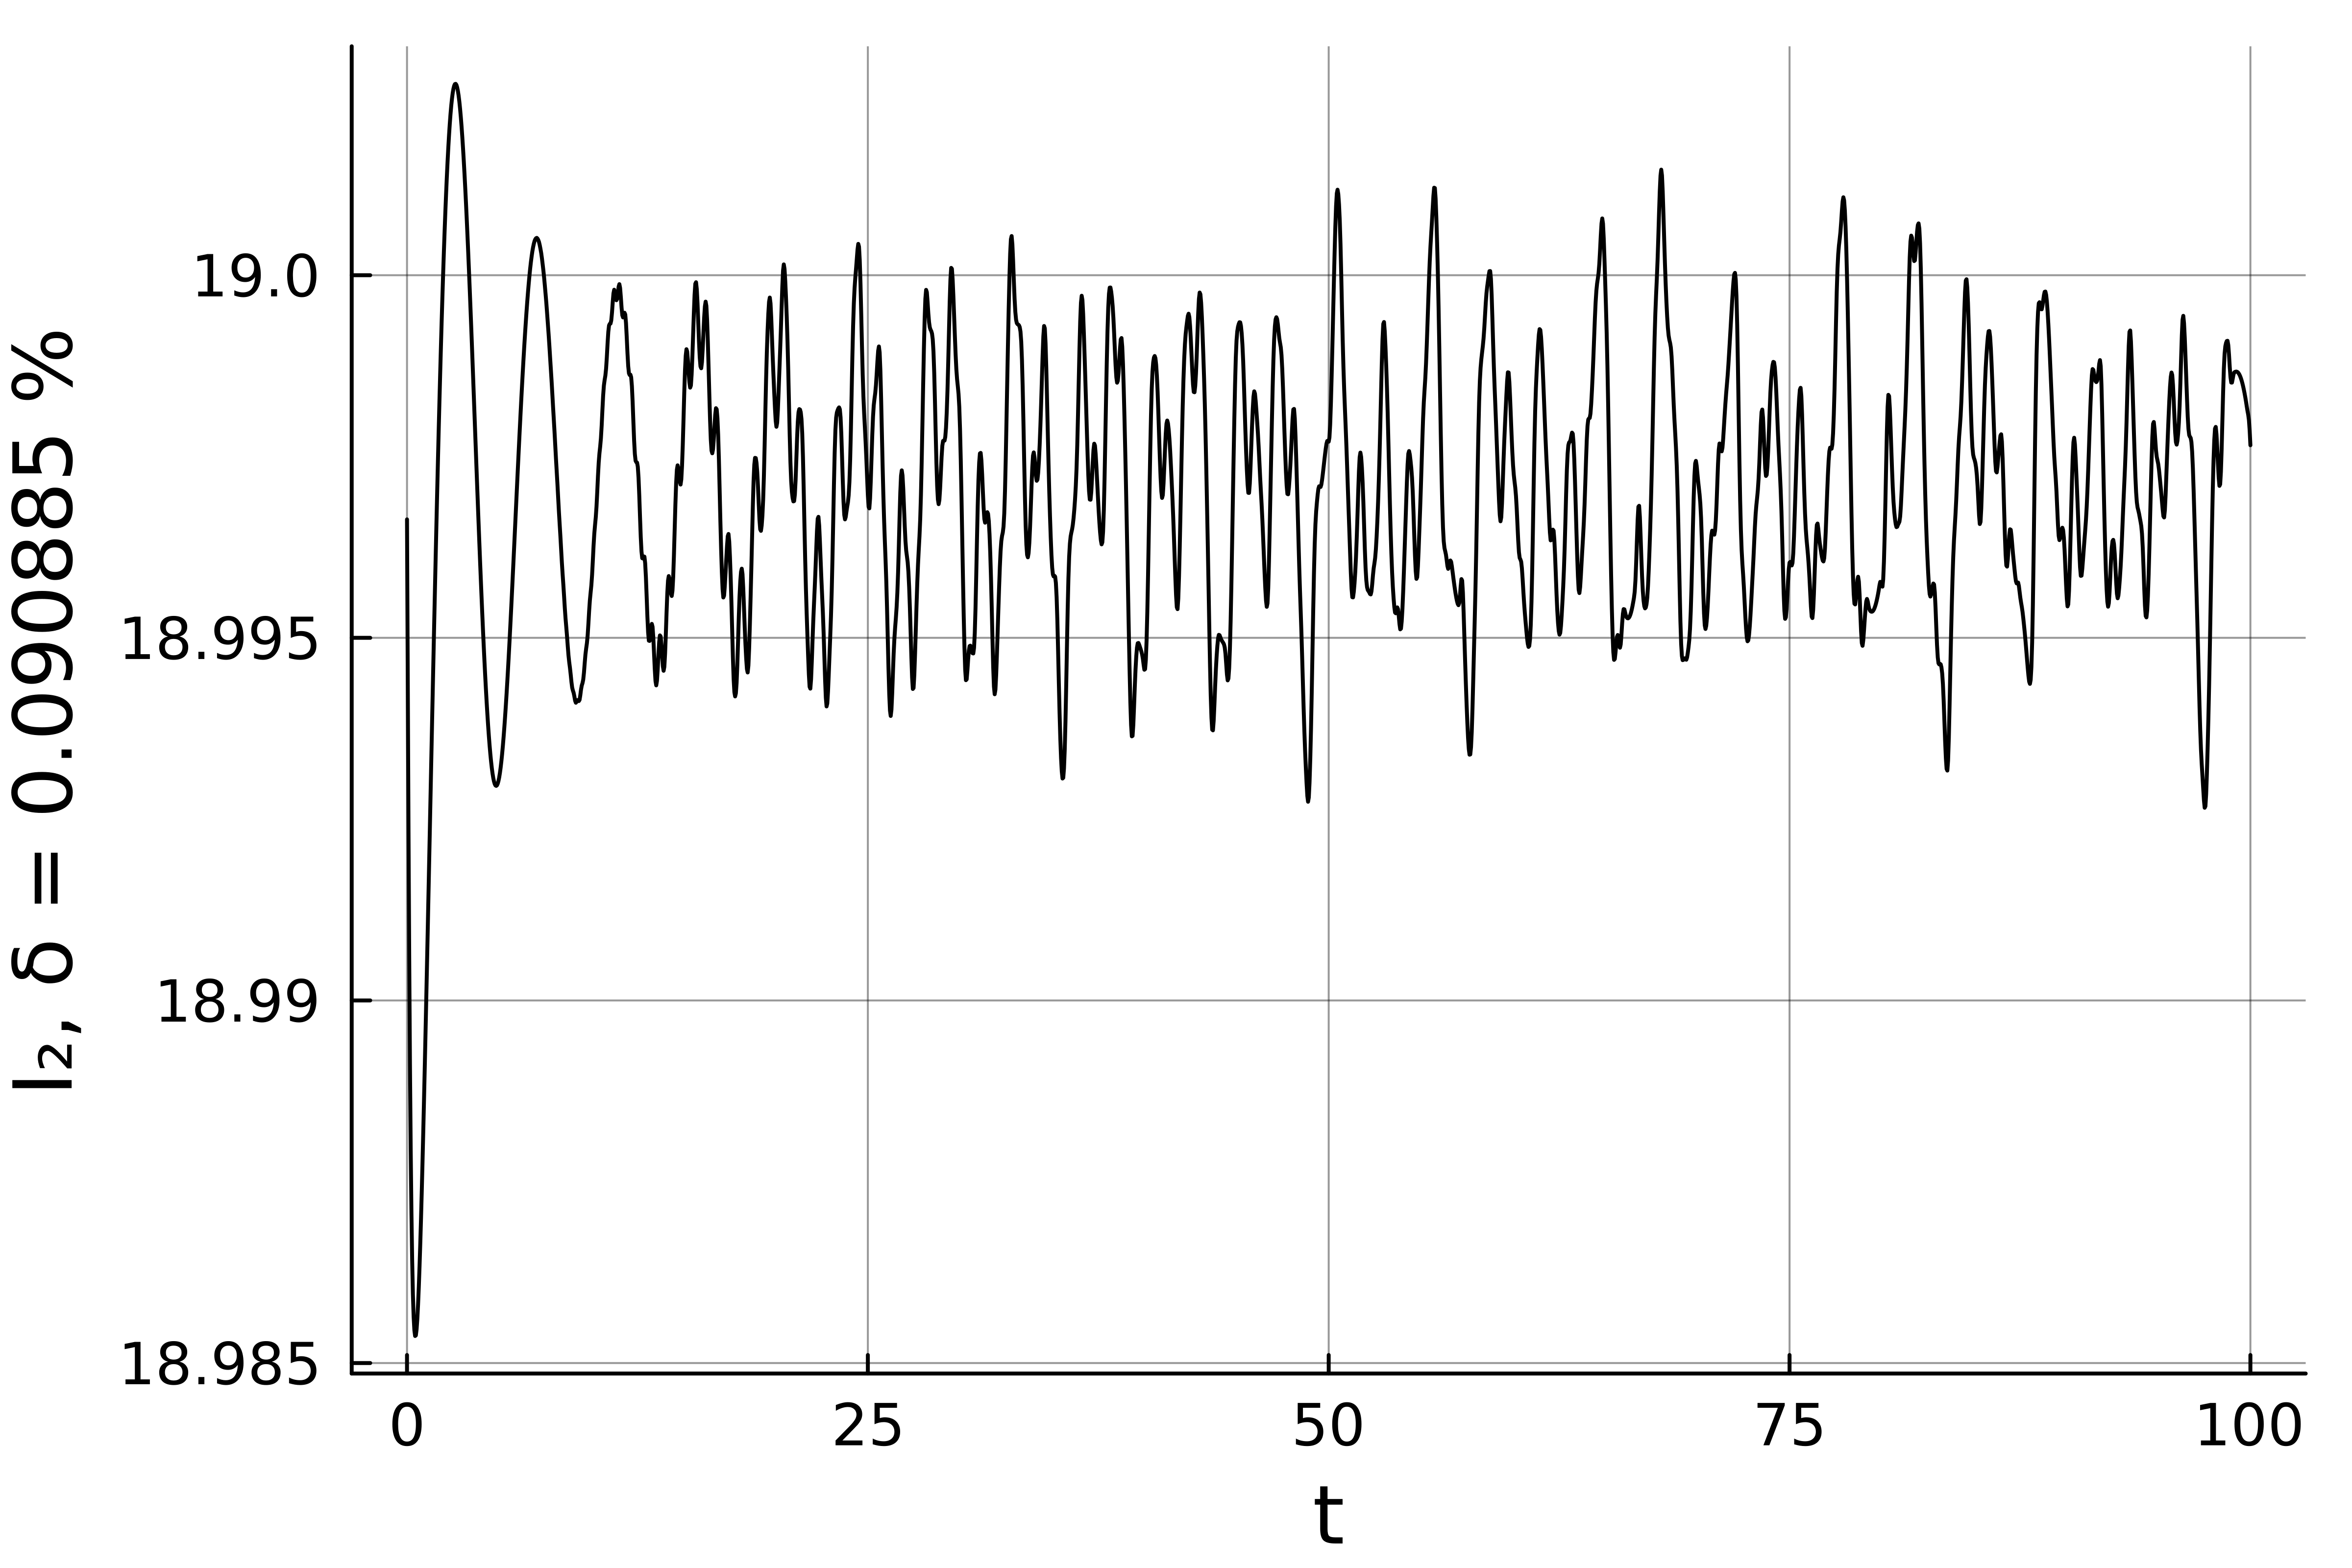
\includegraphics[width=1\linewidth]{fig62.png}
						\subcaption{Зависимость \(I_{2}\) от времени.}
					\end{minipage}
				\end{center}
				\caption{Поведение законов сохранения при
				\(L=100,\, T=100,\, h=0.2,\, \tau=0.04,\)
				\(\varepsilon_{2}=0,\,\varepsilon_{3}=0,\, \omega=1.6,\, k=0.4\).}
				\label{fig340-1}
			\end{figure}

			В случае введения нелинейного члена при \(\varepsilon_{2}\ne 0\), импульс (\ref{eq55}) претерпевает изменения в процессе распространения. Поскольку начальное условие не удовлетворяет уравнению модели (\ref{eq200-4}), солитонные свойства импульса перестают выполняться, и его форма постепенно изменяется. 
			
			Излучение энергии при граничных периодических условиях нарушает изначальное предположение об уединённости импульса, создавая фон из-за периодических граничных условий. Для восстановления справедливости данного предположения, в процесс расчёта введена процедура фильтрации излучения в численном решении. За пределами характерной протяжённости импульса \(l_{f}\) каждые \(t_{f}\) единиц времени расчёта происходит уменьшение численного решения в \(k_{f}\) раз. При \(k_{f}=1\) численное решение не изменяется. Результат фильтрации проиллюстрирован на Рис.\ref{340-2}. Алгоритм поддерживает задание динамического коэффициента \(k_{f}\left(t\right)\), что позволяет отключить диссипацию излучения на произвольных временах моделирования.
			\begin{figure}[H] %% color here
				\begin{center}
					\begin{minipage}[h]{0.48\linewidth}
						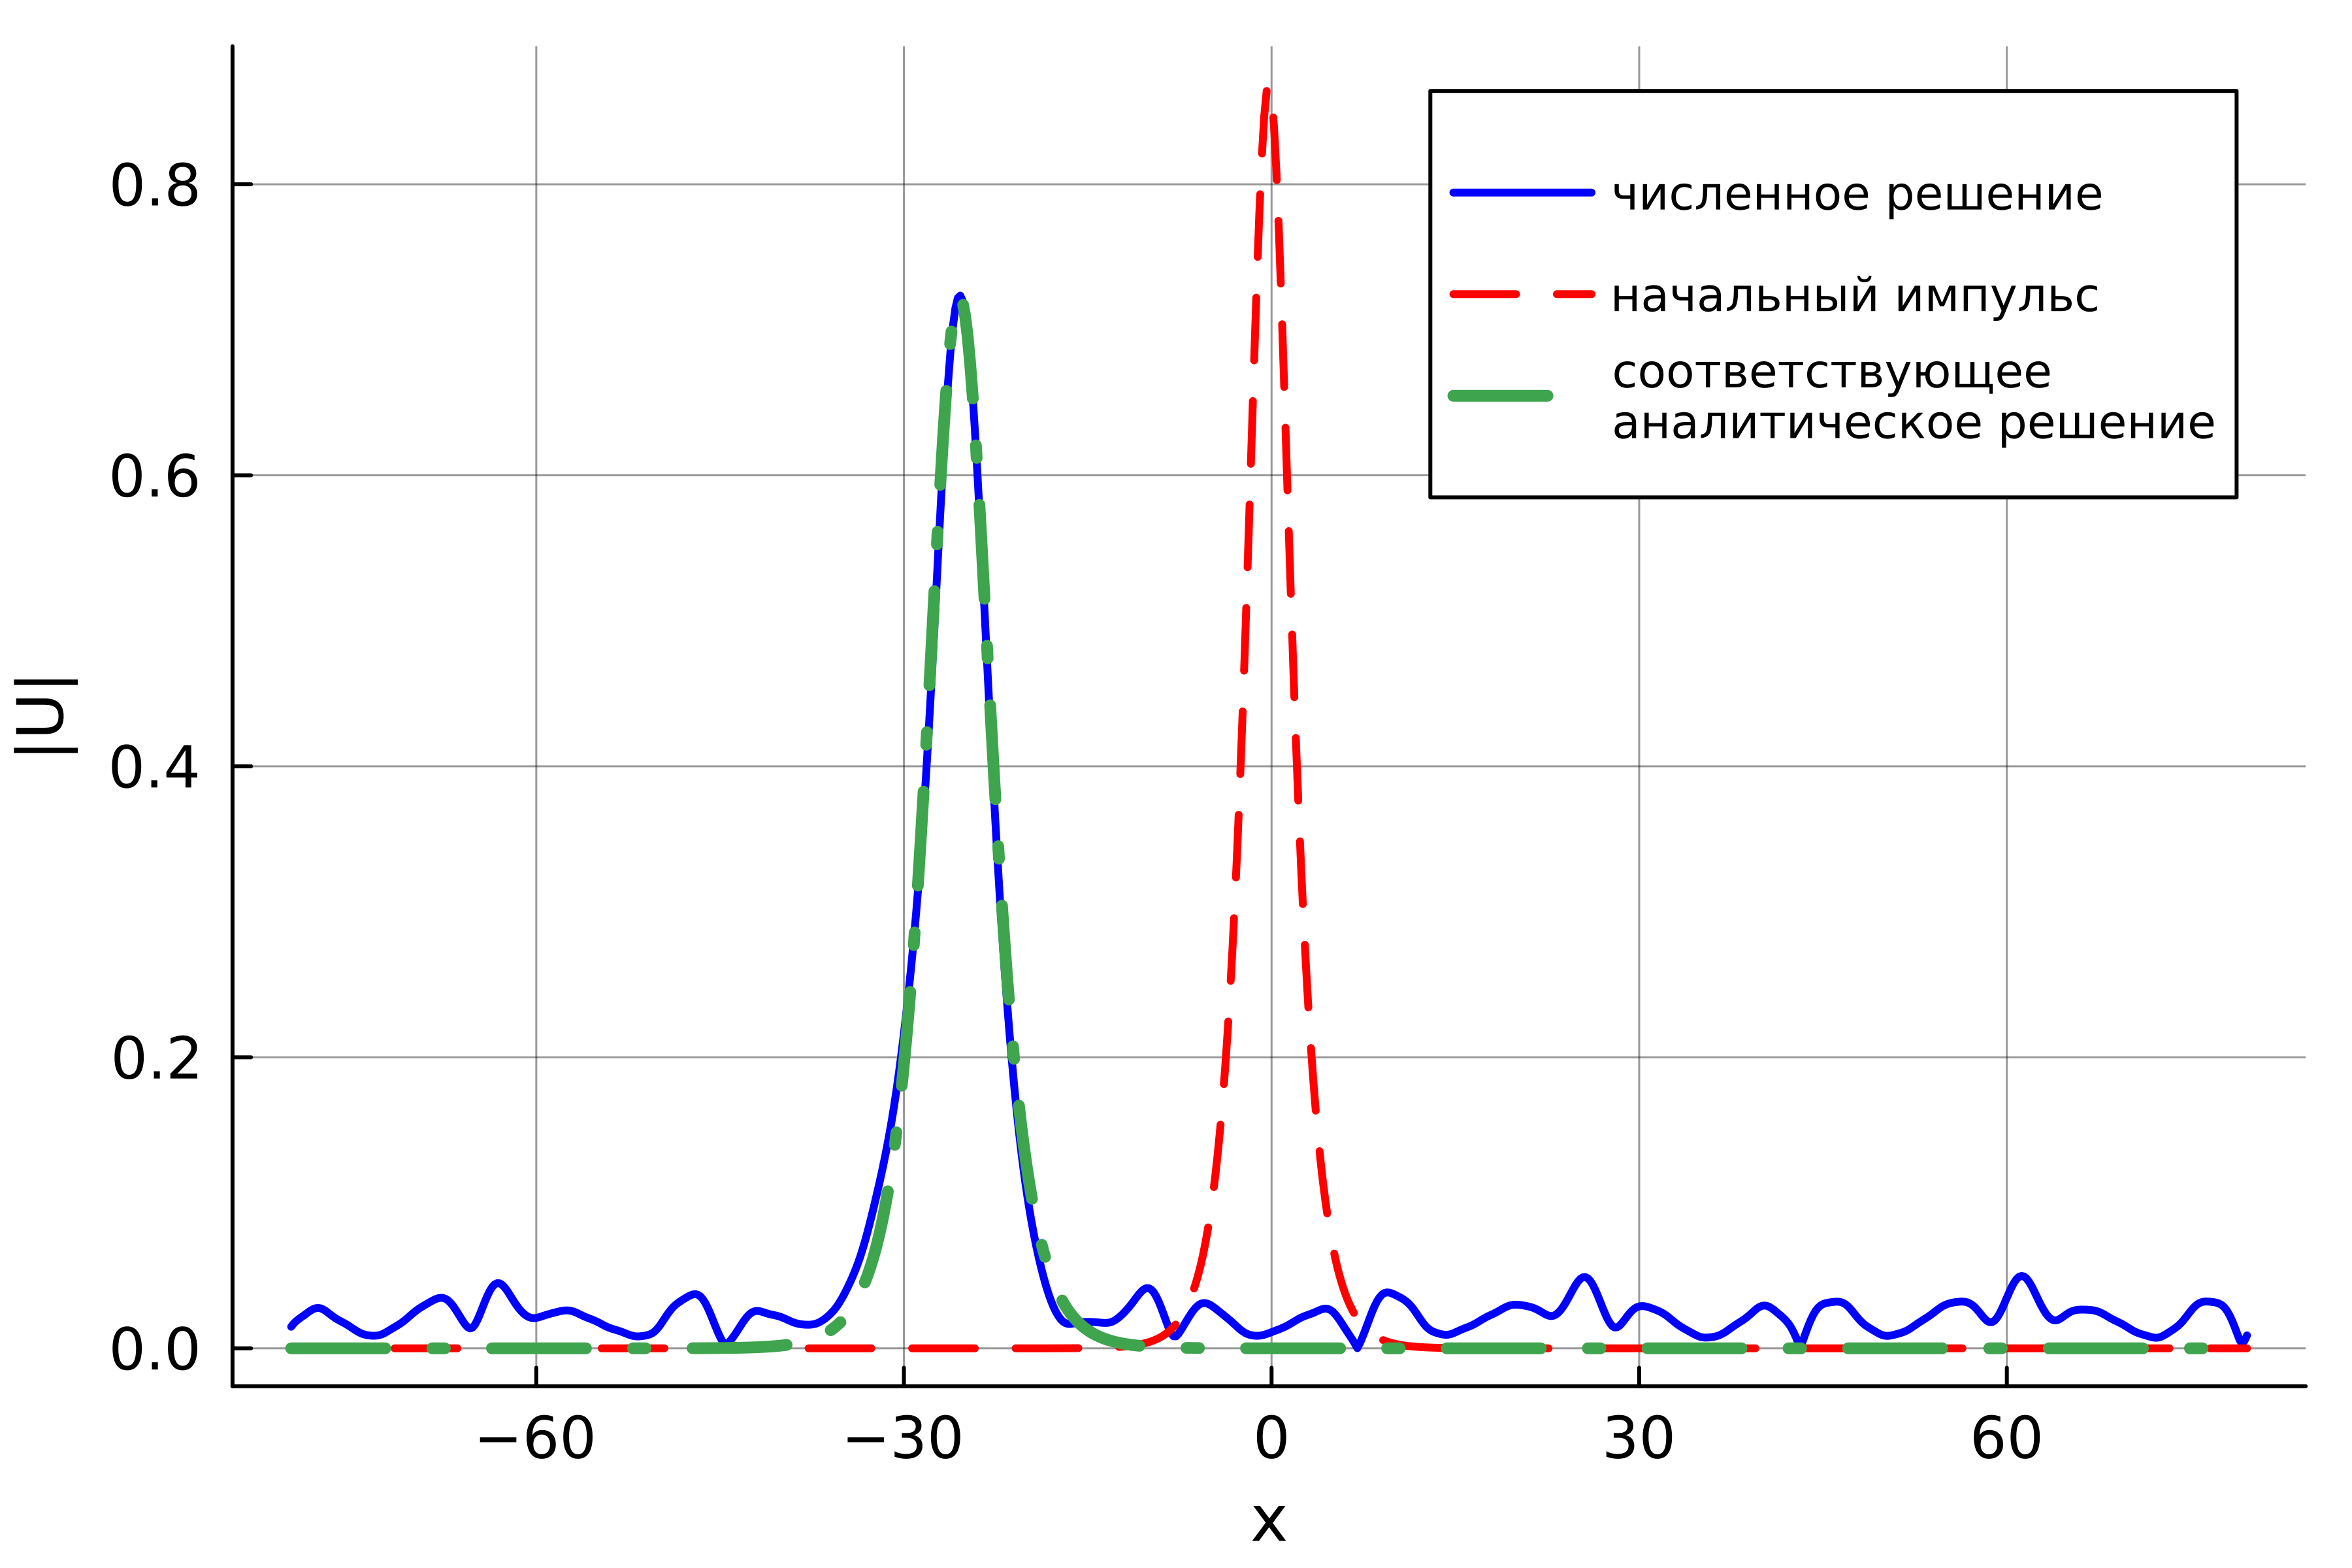
\includegraphics[width=1\linewidth]{fig63.png}
						\subcaption{Профиль решения при t=450 без применения фильтрации}
					\end{minipage}
					\hfill
					\begin{minipage}[h]{0.48\linewidth}
						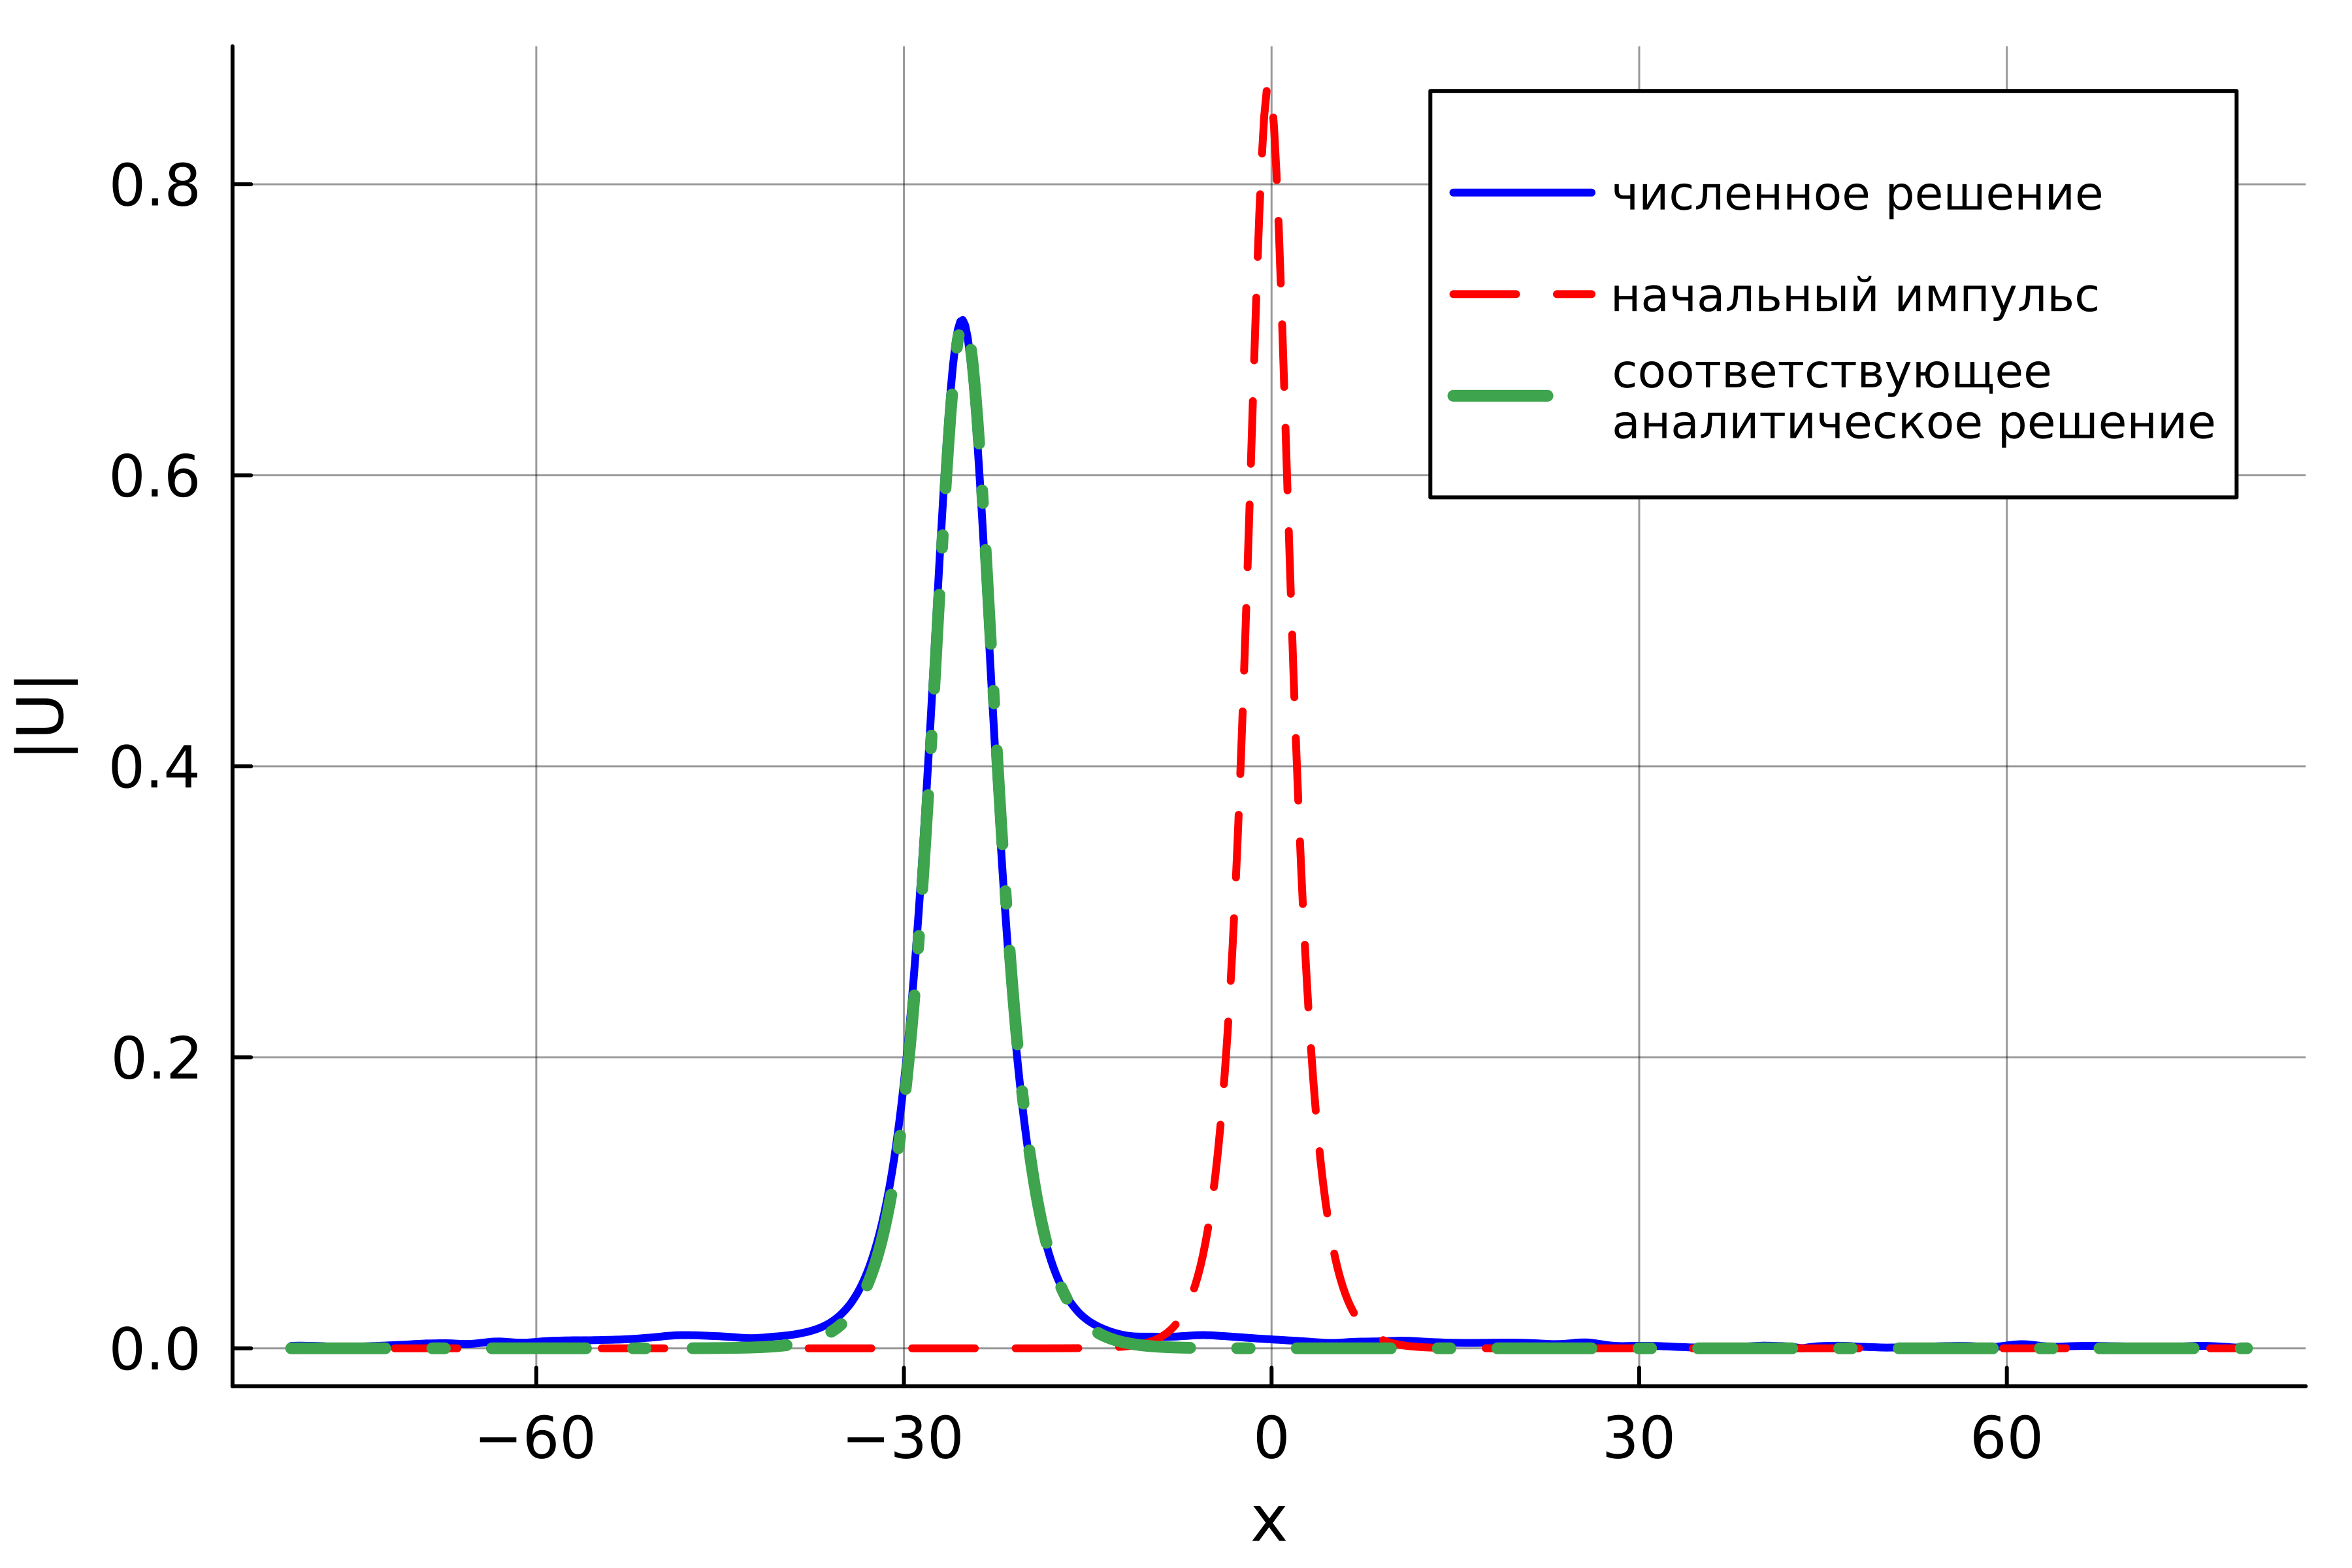
\includegraphics[width=1\linewidth]{fig64.png}
						\subcaption{Профиль решения при t=450 с применением фильтрации}
					\end{minipage}
				\end{center}
				\caption{Численные результаты распространения импульса (\ref{eq55}) при
				\(L=160,\, T=450,\, h=0.2,\, \tau=0.04,\,l_{f}=60,\, t_{f}=2, \, k_{f}=1.02\)
				\(\varepsilon_{2}=-0.5,\,\varepsilon_{3}=0,\, \omega=0.4,\, k=0.15\).}
				\label{340-2}
			\end{figure}

			Обнаружено, что форма импульса (\ref{eq55}) в процессе расчёта становится устойчивой. По мере моделирования амплитуда солитона стремится к равновесному значению, а его форма - к соответствующему для данной амплитуды решению вида (\ref{e7}), являющимся аналитическим для обобщённой модели при \(\varepsilon_{2}\ne 0\). Для расчёта, проиллюстрированного на Рис. \ref{fig21_1} и Рис. \ref{fig21_2} максимальная относительная ошибка между численным и аналитическим решением в конечный момент времени моделирования при \(T=3500\) не превышает 0.05\%.
			\begin{figure}[H] %% color here
				\begin{center}
					\begin{minipage}[h]{0.48\linewidth}
						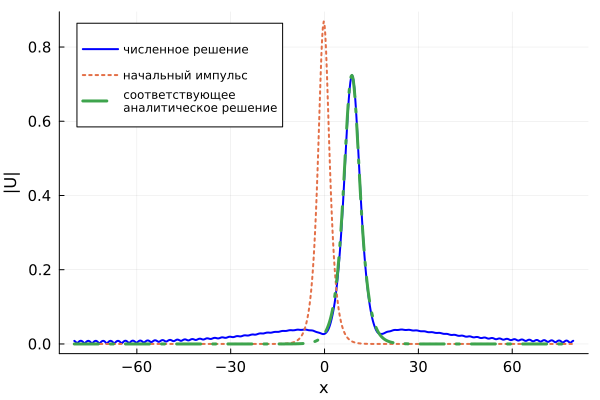
\includegraphics[width=1\linewidth]{Medvedev_fig10.png}
						\subcaption{Профиль решения при t=30}
					\end{minipage}
					\hfill
					\begin{minipage}[h]{0.48\linewidth}
						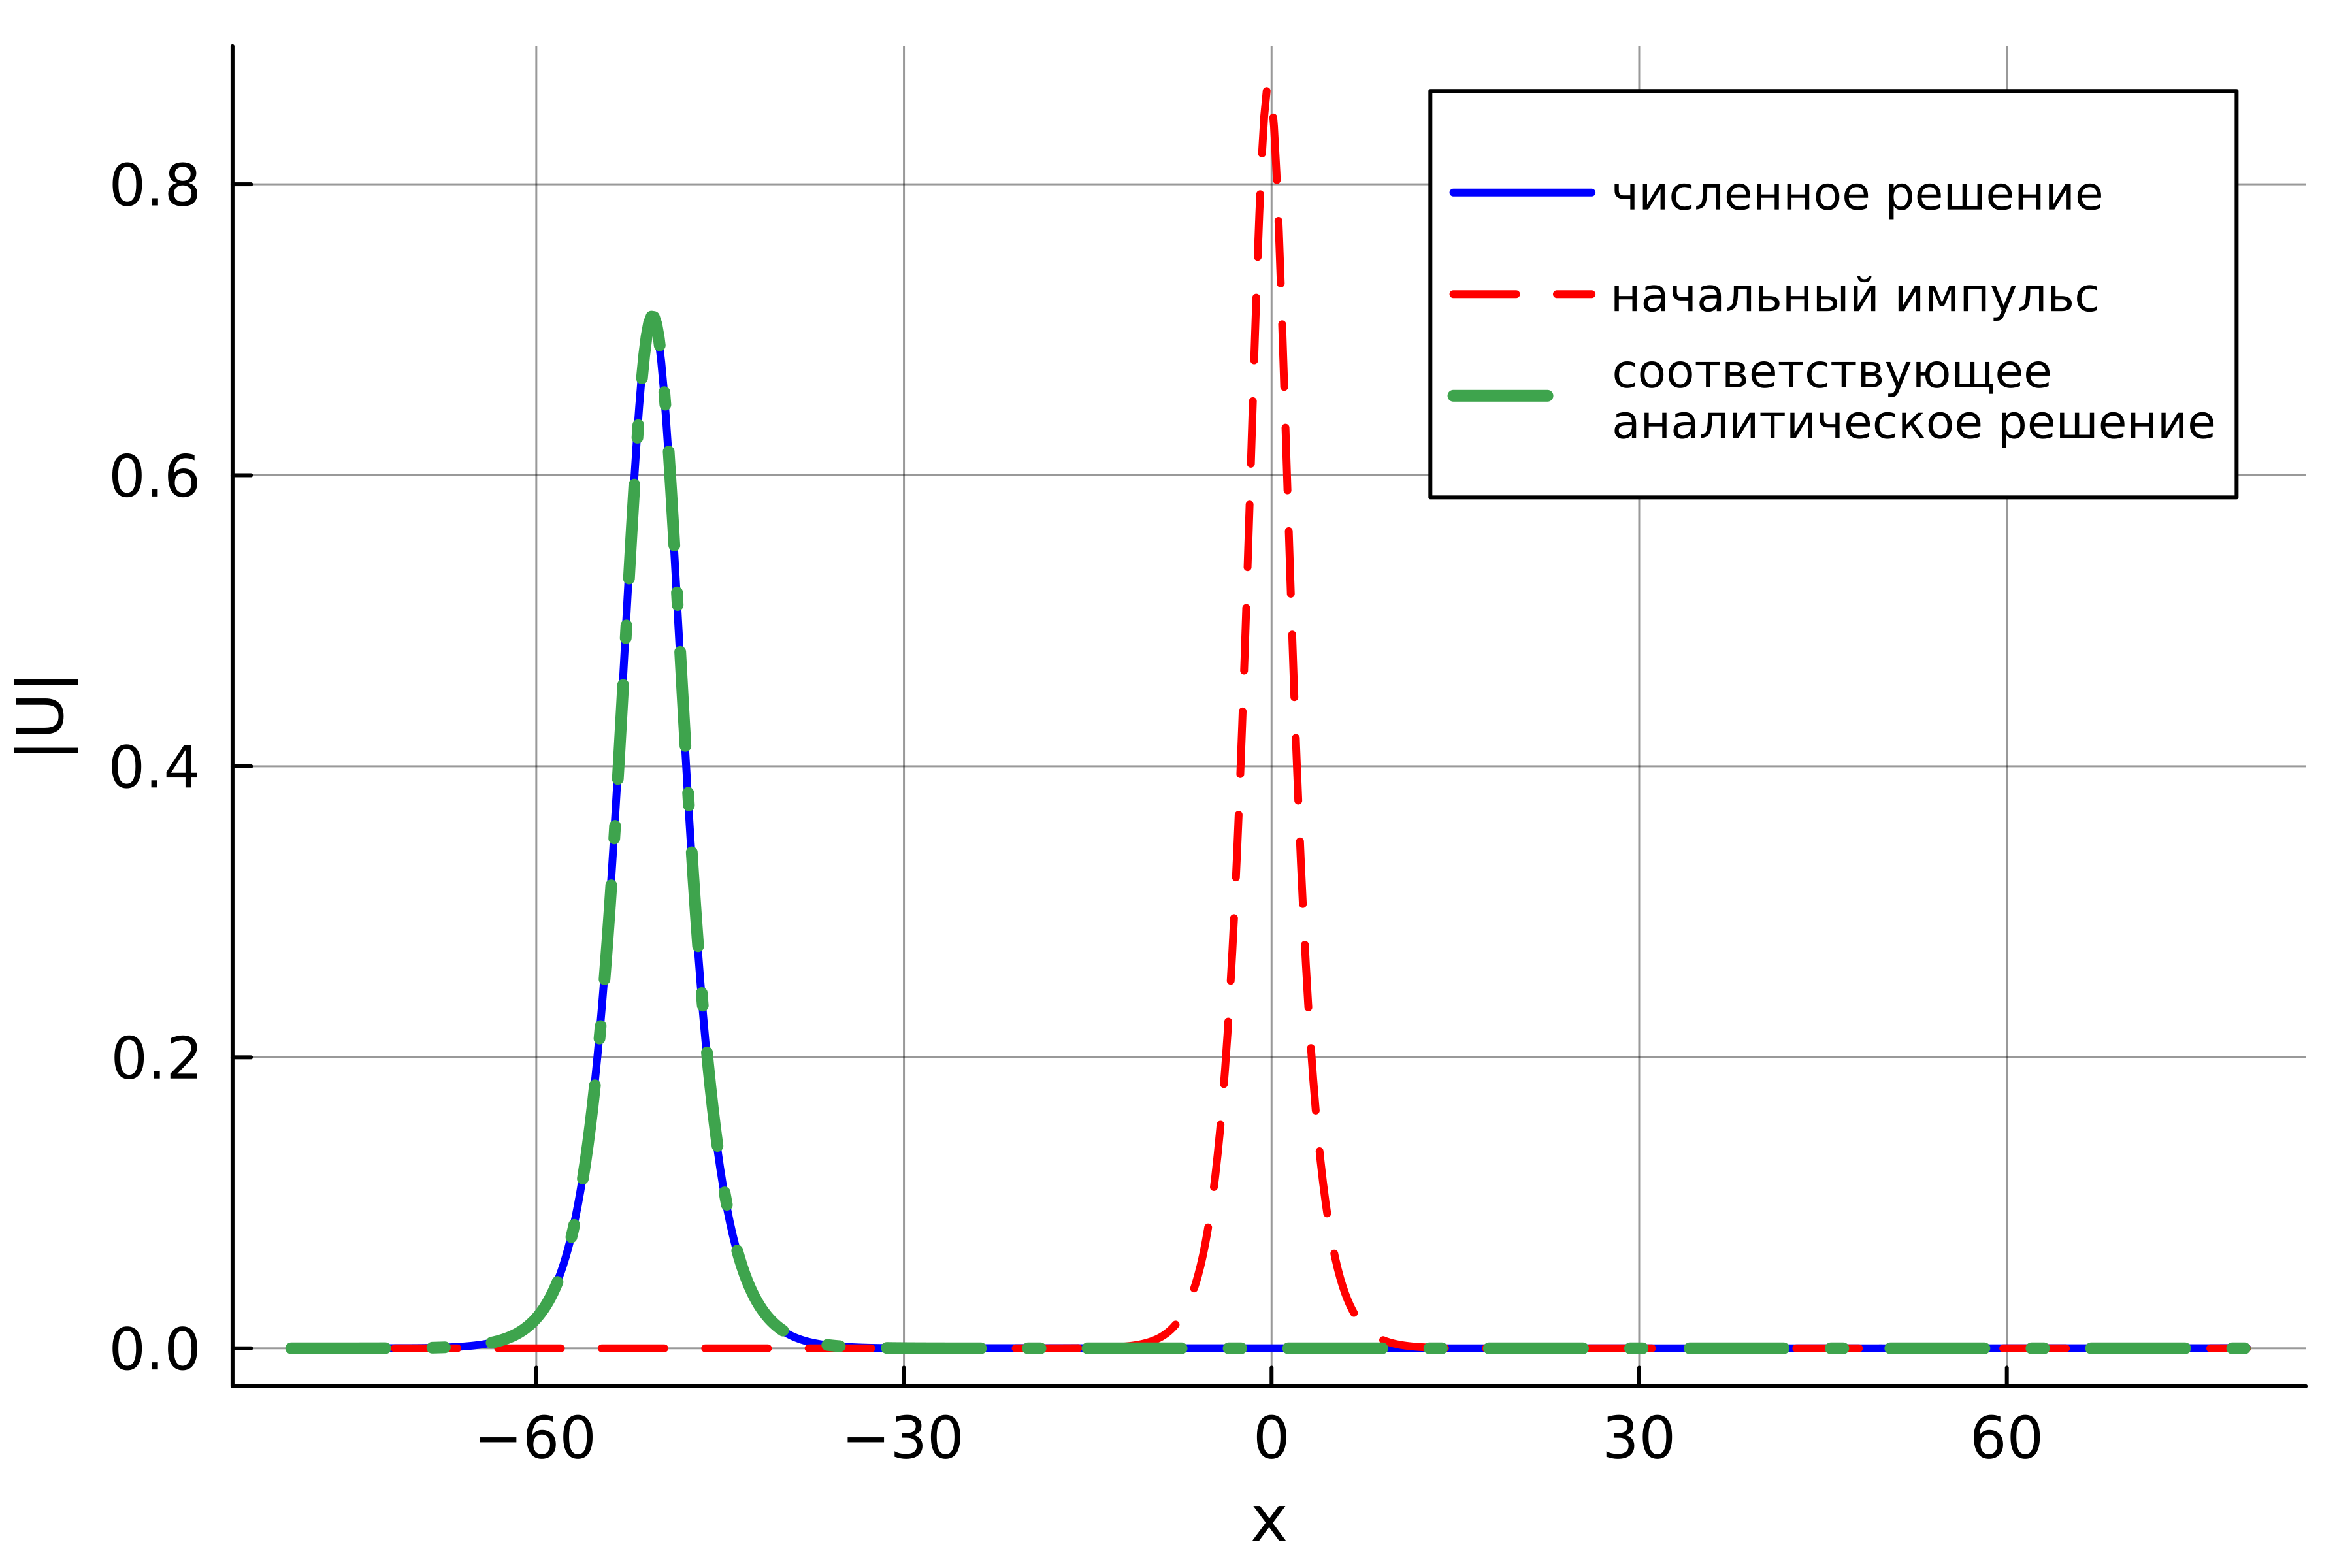
\includegraphics[width=1\linewidth]{Medvedev_fig19.png}
						\subcaption{Профиль решения при t=3500}
					\end{minipage}
				\end{center}
				\caption{Численные результаты распространения импульса (\ref{eq55}) при
				\(L=160,\, T=3500,\, h=0.2,\, \tau=0.04,\)
				\(\varepsilon_{2}=-0.5,\,\varepsilon_{3}=0,\, \omega=0.4,\, k=0.15\).}
				\label{fig21_1}
			\end{figure}

			Зависимость относительной ошибки между аналитическим (\ref{e7}) и численным решением от времени представлена на Рис. \ref{fig21_2}. Зависимость коэффициента фильтрации от времени также проиллюстрирована на графике. Коэффициент \(k_{f}\left(t\right)\) линейно убывает в процессе моделирования, и равен \(k_{f}=1\) при \(t=2500\). Подбор аналитического решения происходит по максимуму модуля численного решения и параметру \(\varepsilon_{2}\). Для снижения сеточной ошибки при построении аналитического решения по численному, максимум модуля импульса определяется в результате решения задачи поиска глобального максимума B-сплайновой функции интерполяции, построенной для сеточного решения.

			\begin{figure}[H]
				\begin{center}
					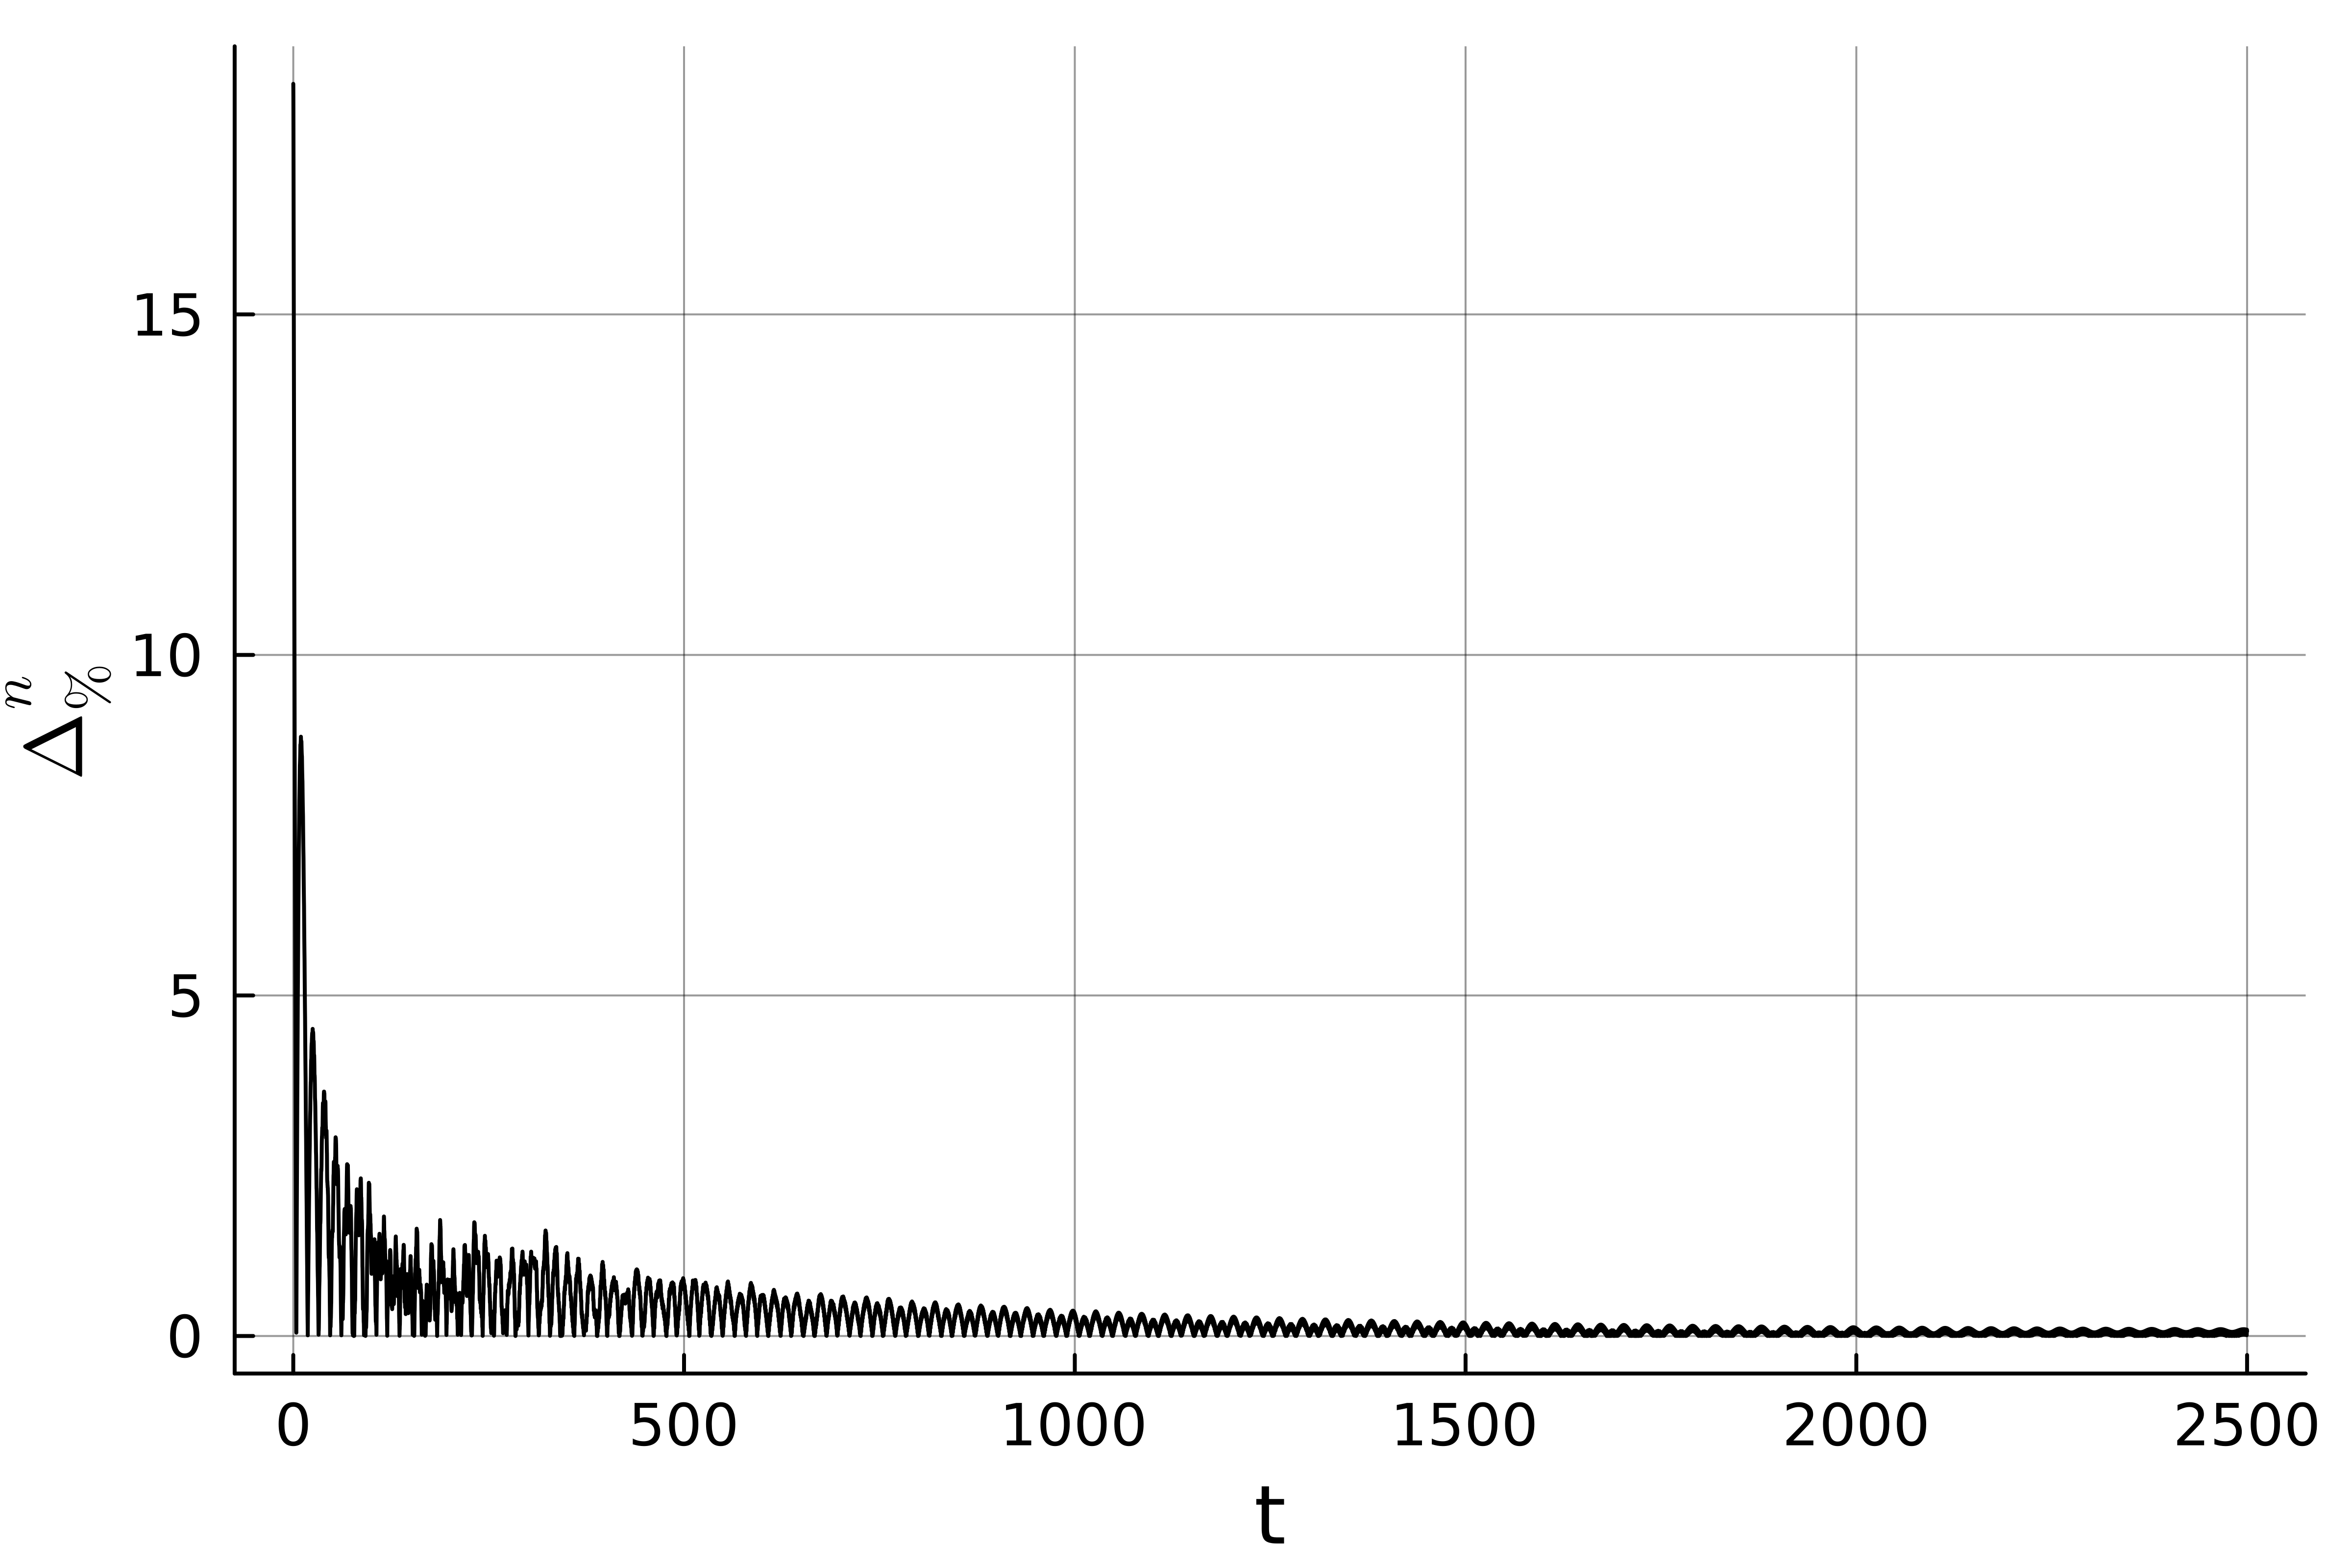
\includegraphics[width=0.5\linewidth]{Medvedev_fig18.png}
					\subcaption{}
				\end{center}
				\caption{Зависимости относительной ошибки и коэффициента фильтрации от времени при
				\(L=160,\, T=3500,\, h=0.2,\, \tau=0.04,\)
				\(\varepsilon_{2}=-0.5,\,\varepsilon_{3}=0,\, \omega=0.4,\, k=0.15\).}
				\label{fig21_2}
			\end{figure}

			Поведение законов сохранения для представленного моделирования проиллюстрировано на Рис. \ref{fig340-5}. Солитоном потеряно 3.6\% мощности и импульса, однако с учётом рассеянных составляющих оба интеграла сохраняются, что говорит о корректном применении процедуры фильтрации и выполнении законов сохранения. Величина \(\delta\) на Рис. \ref{fig340-5} равна относительной точности, с которой в процессе всего моделирования сохраняются величины \(I_{1}+I_{1f}\) и \(I_{2}+I_{2f}\), где \(I_{1f}\) и \(I_{2f}\) - рассеянные компоненты мощности и импульса.
			\begin{figure}[H] %% color here
				\begin{center}
					\begin{minipage}[h]{0.48\linewidth}
						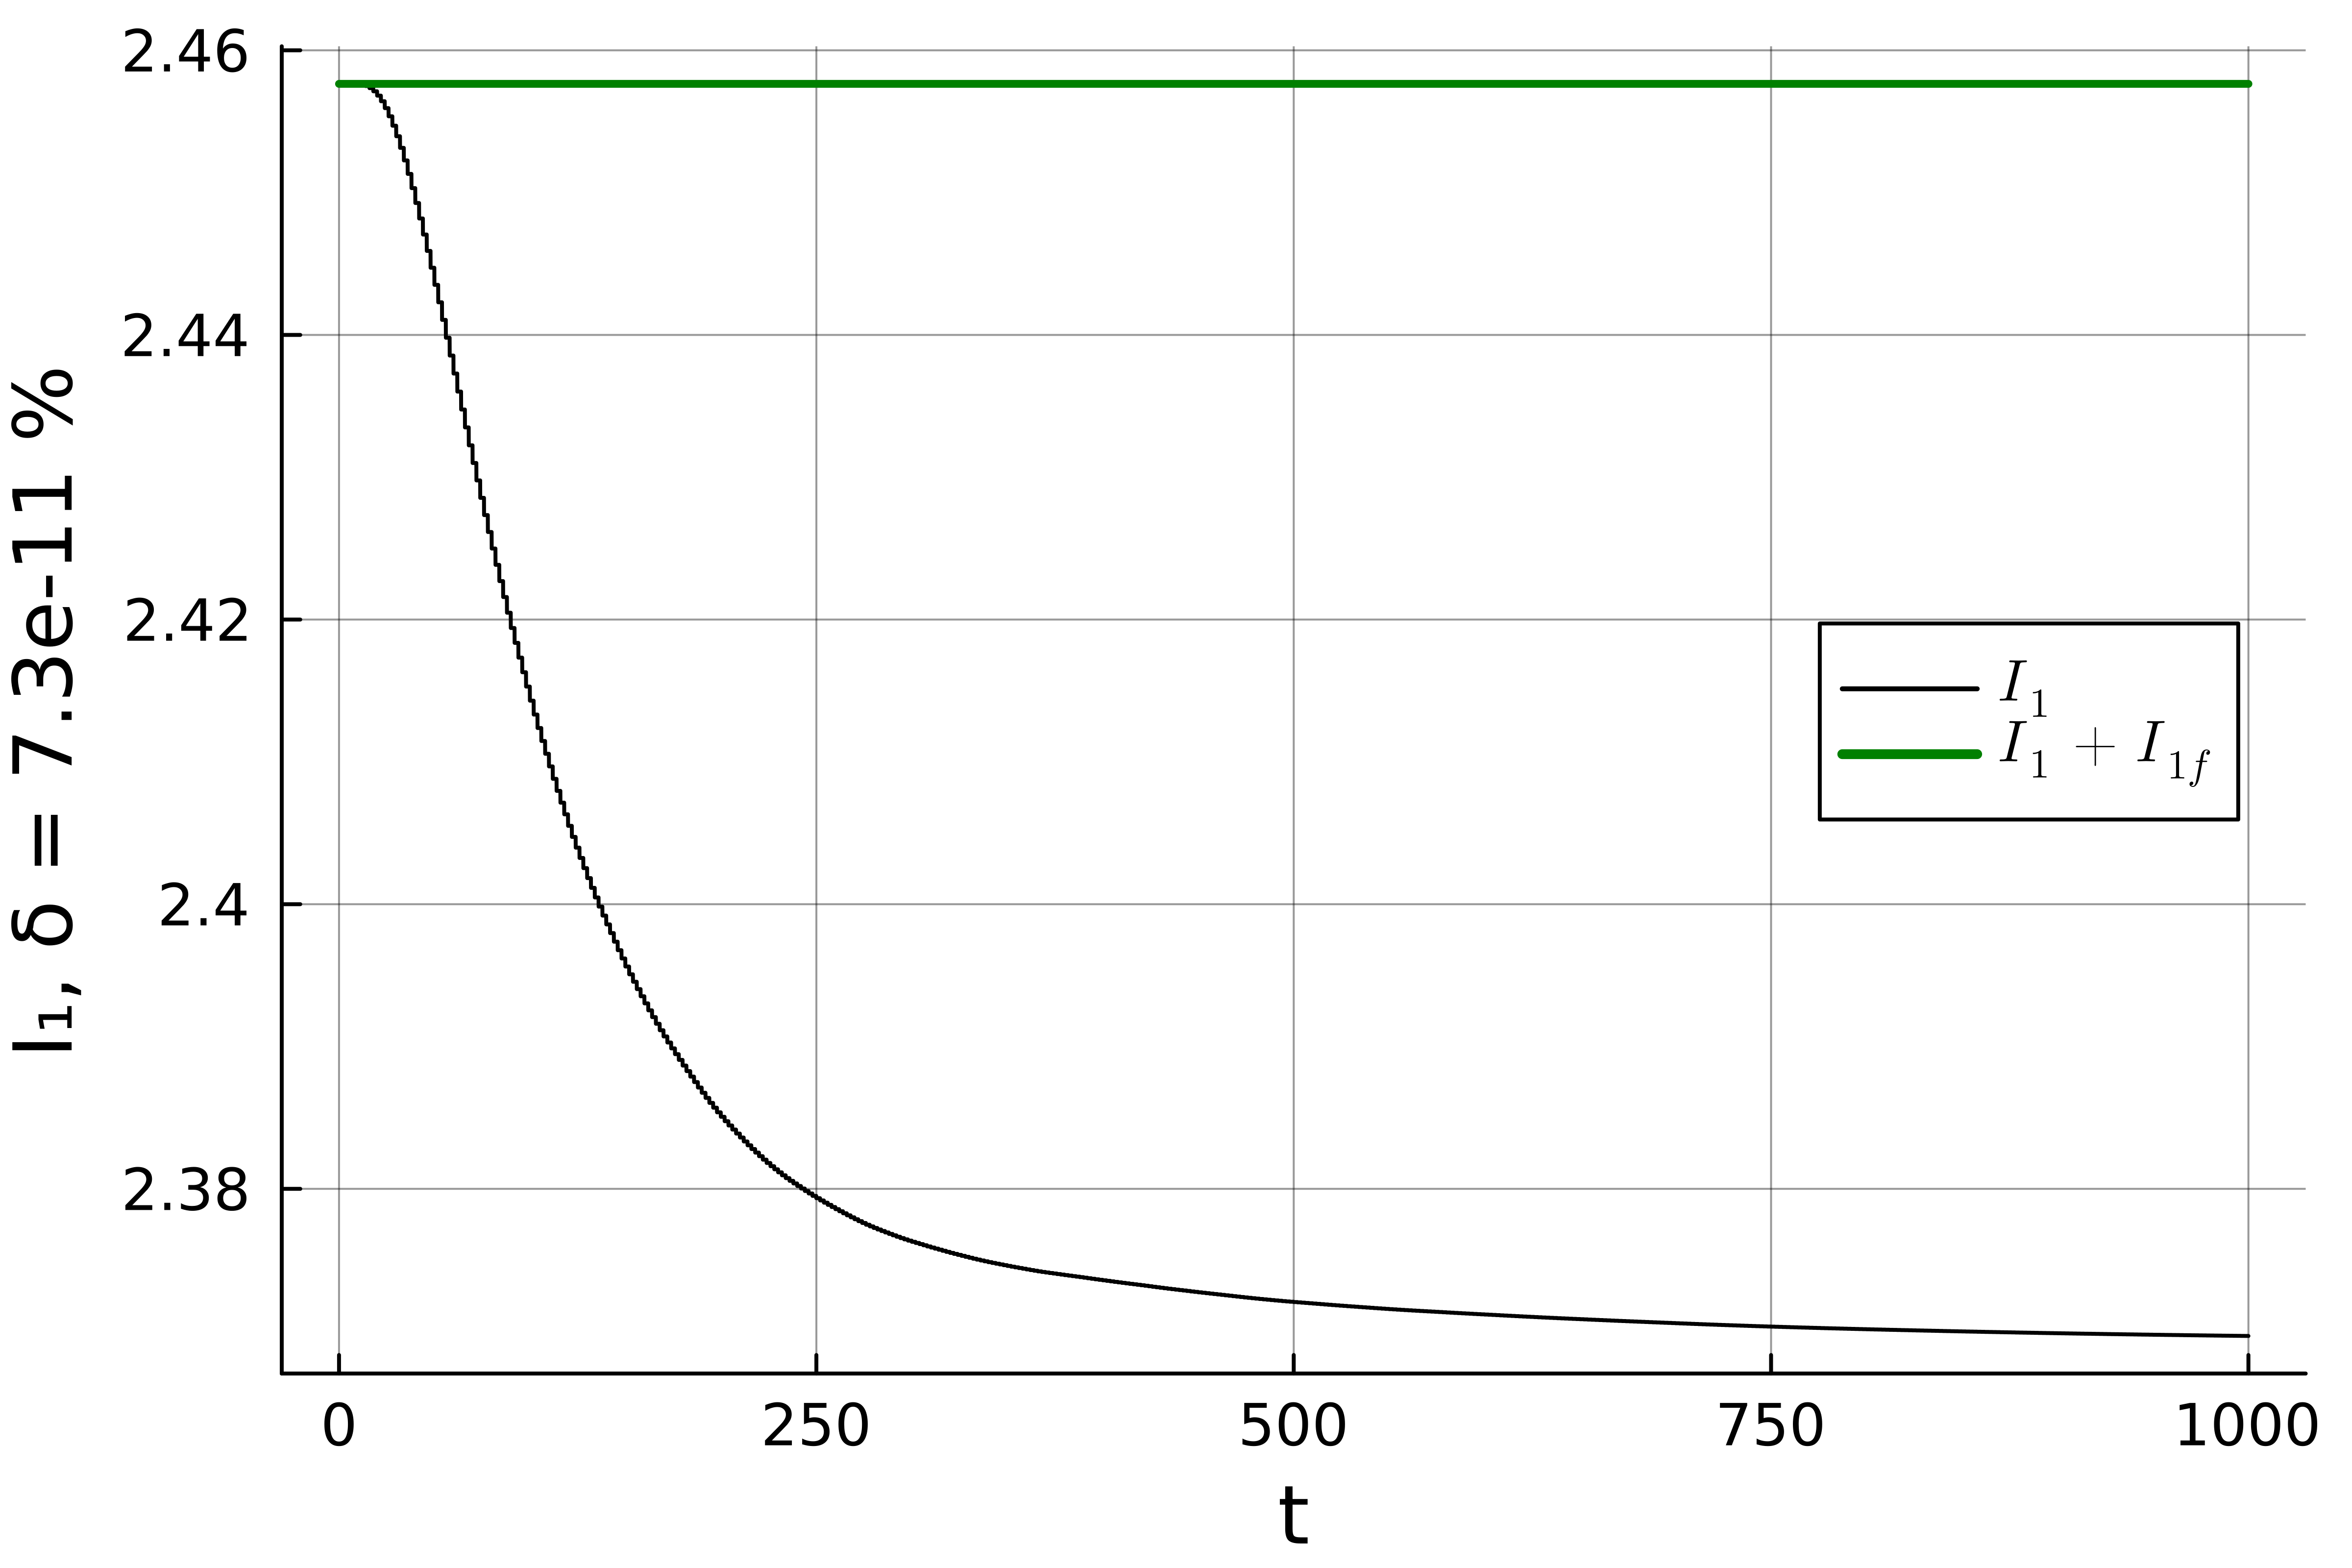
\includegraphics[width=1\linewidth]{fig65.png}
						\subcaption{Зависимость \(I_{1}\) от времени.}
					\end{minipage}
					\hfill
					\begin{minipage}[h]{0.48\linewidth}
						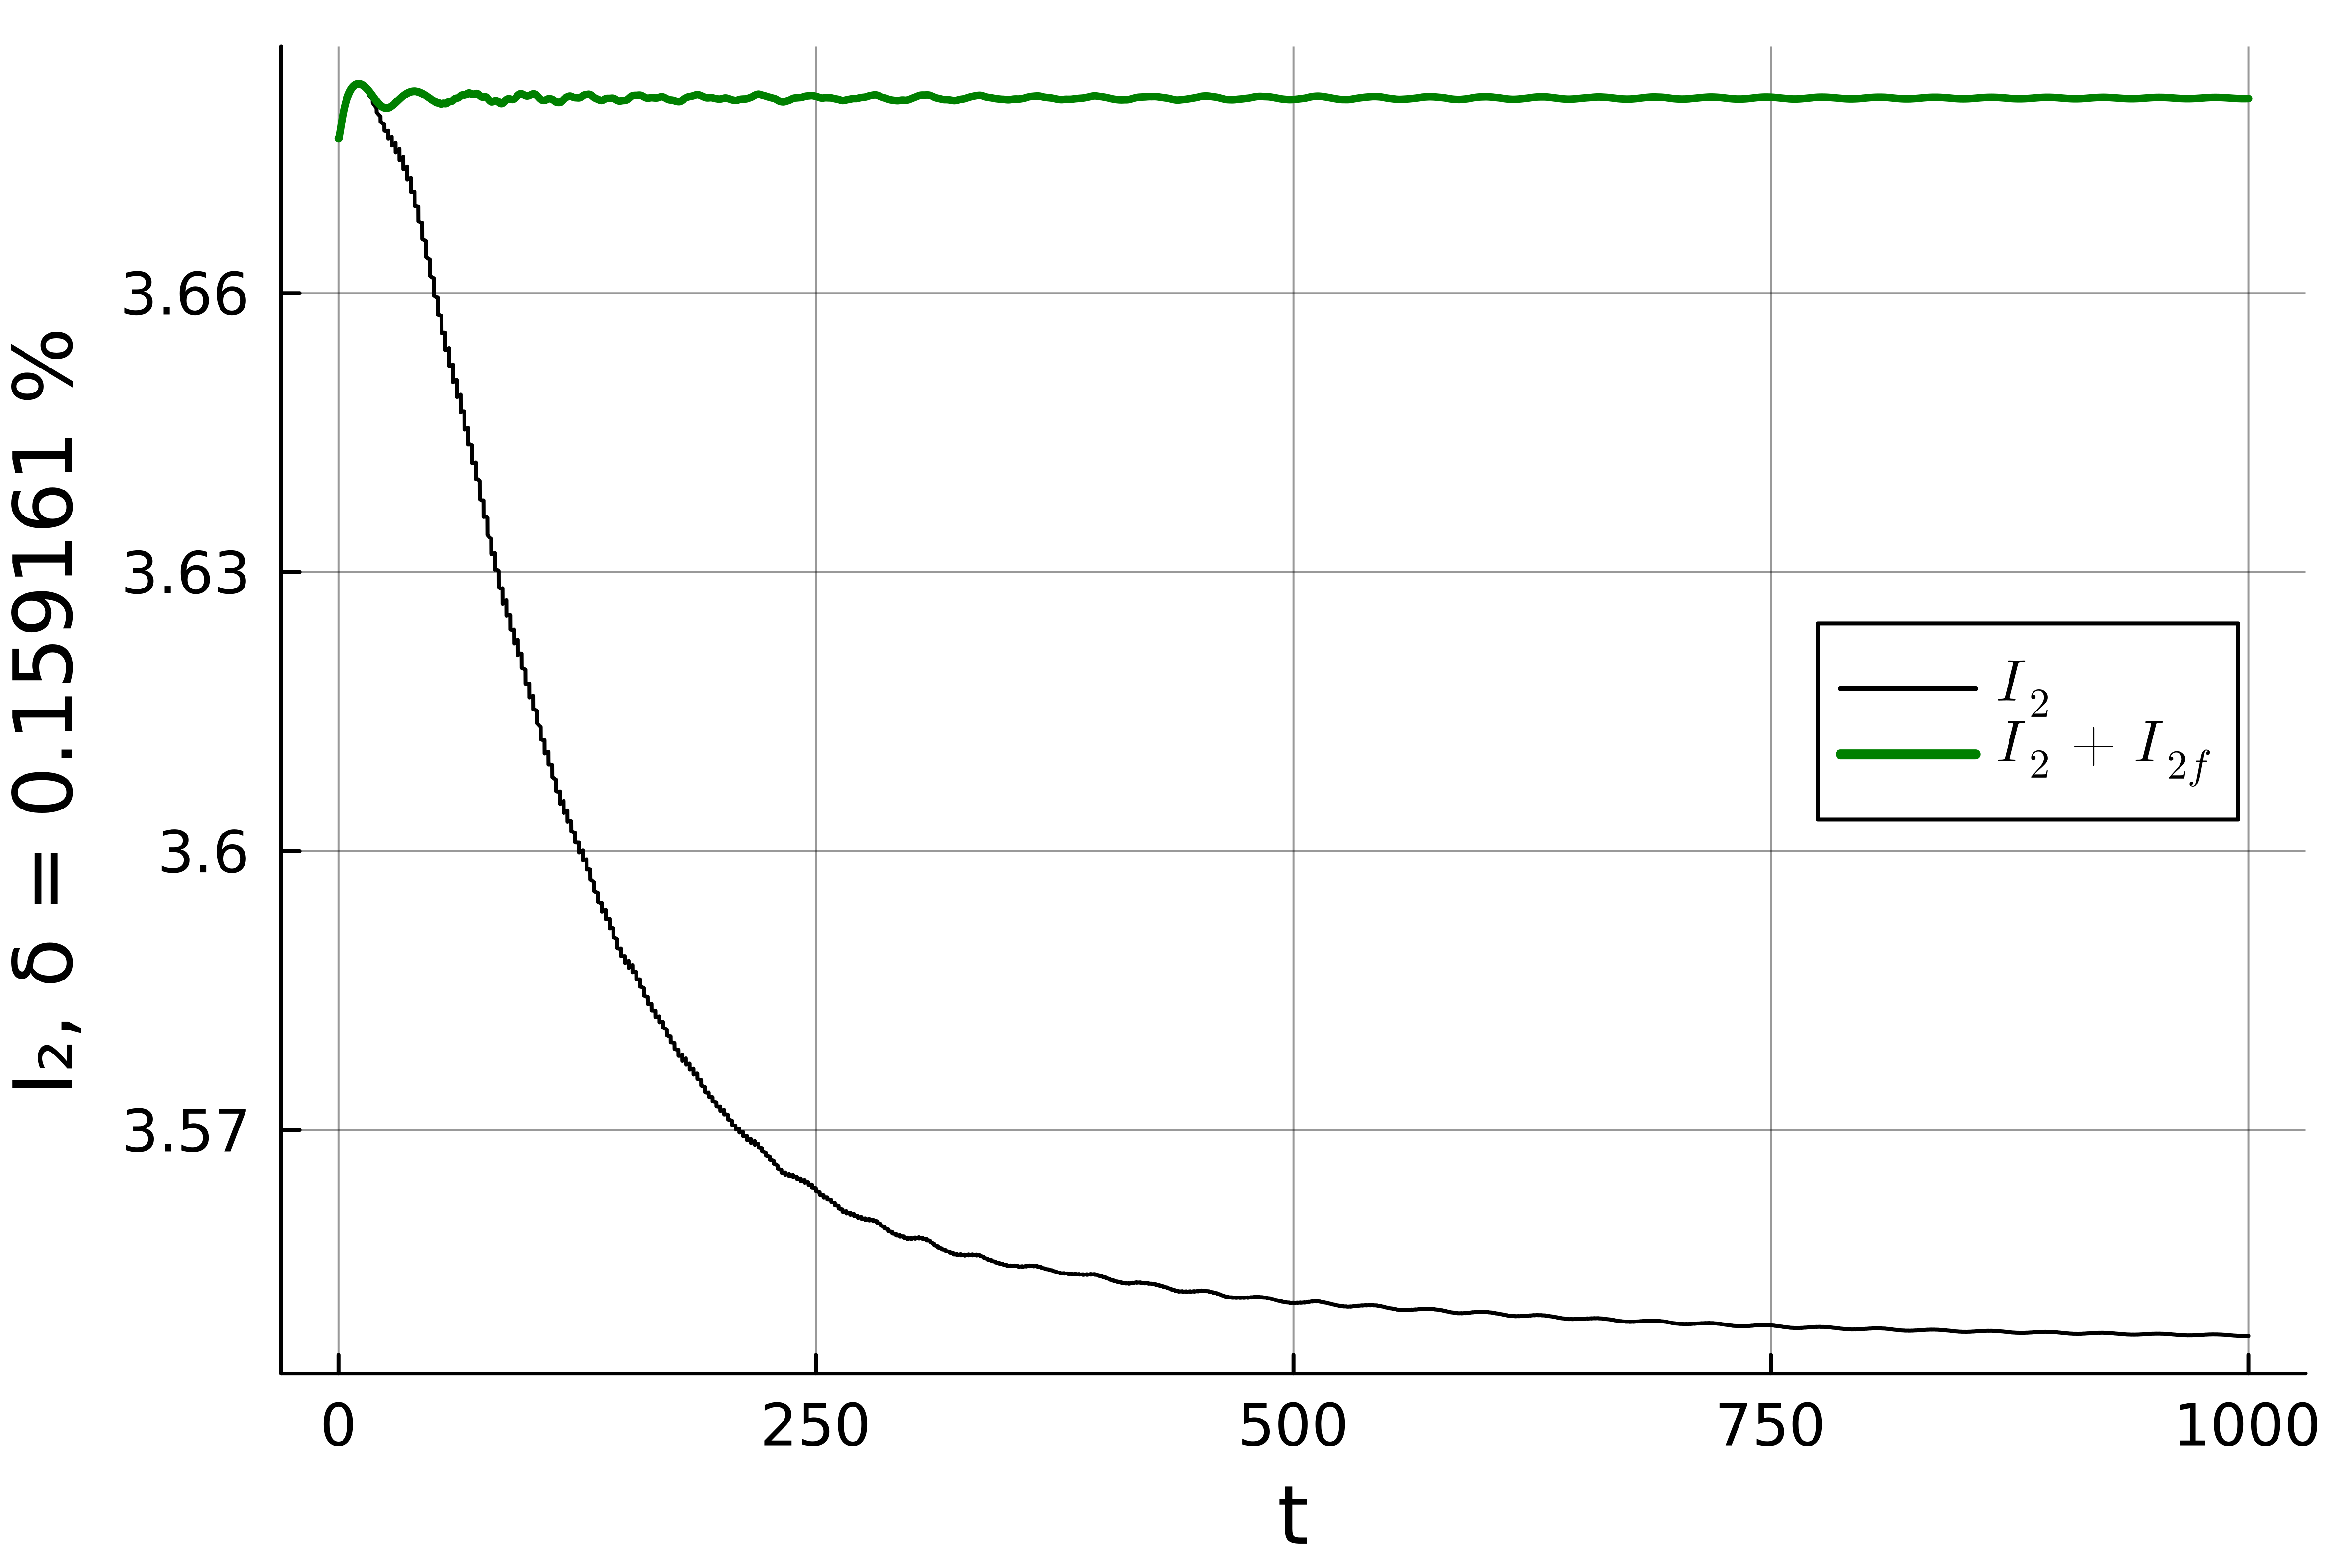
\includegraphics[width=1\linewidth]{fig66.png}
						\subcaption{Зависимость \(I_{2}\) от времени.}
					\end{minipage}
				\end{center}
				\caption{Поведение законов сохранения при
				\(L=160,\, T=1000,\, h=0.2,\, \tau=0.04,\)
				\(\varepsilon_{2}=-0.5,\,\varepsilon_{3}=0,\, \omega=0.4,\, k=0.15\).}
				\label{fig340-5}
			\end{figure}
			Отметим, что более длительная фильтрация позволяет добиться на порядок меньшей ошибки между численным и аналитическим решением. Так, при времени окончания фильтрации \(t_{end,f}=T=5000\) и линейном убывающем к единице законе изменения \(k_{f}\left(t\right)\) в конечный момент времени максимальная относительная разница аналитического и численного решений составляет 0.002\%. При увеличении времени моделирования и конца фильтрации в два раза дополнительно рассеялось \(4e^{-4}\%\) от \(I_{1}\) и \(2e^{-4}\%\) от \(I_{2}\), что говорит о том, что импульс во второй половине моделирования потерял в \(8700\) раз меньше мощности и в \(17000\) раз меньше импульса, чем в первой. Данное наблюдение позволяет заключить, что исходный импульс под влиянием нелинейных выражений в модели преобразуется в другой импульс меньшей амплитуды, совпадающий с аналитическим решением (\ref{e7}) уравнения (\ref{eq200-4}) при \(\varepsilon_{3}=0\). Данный процесс устанавливается со временем.

			Выводы, полученные выше, справедливы для \(\varepsilon_{2}<0\). Чем меньше при этом абсолютное значение параметра \(\varepsilon_{2}\), тем меньше потерь импульсом на излучение, и тем меньше изменяется его амплитуда. Зависимости процентной величины потерь и амплитуды установившегося импульса от параметра нелинейности для отдельно взятых параметров модели и сетки проиллюстрирована на Рис. \ref{fig340-5_1}
			\begin{figure}[H] %% color here
				\begin{center}
					\begin{minipage}[h]{0.48\linewidth}
						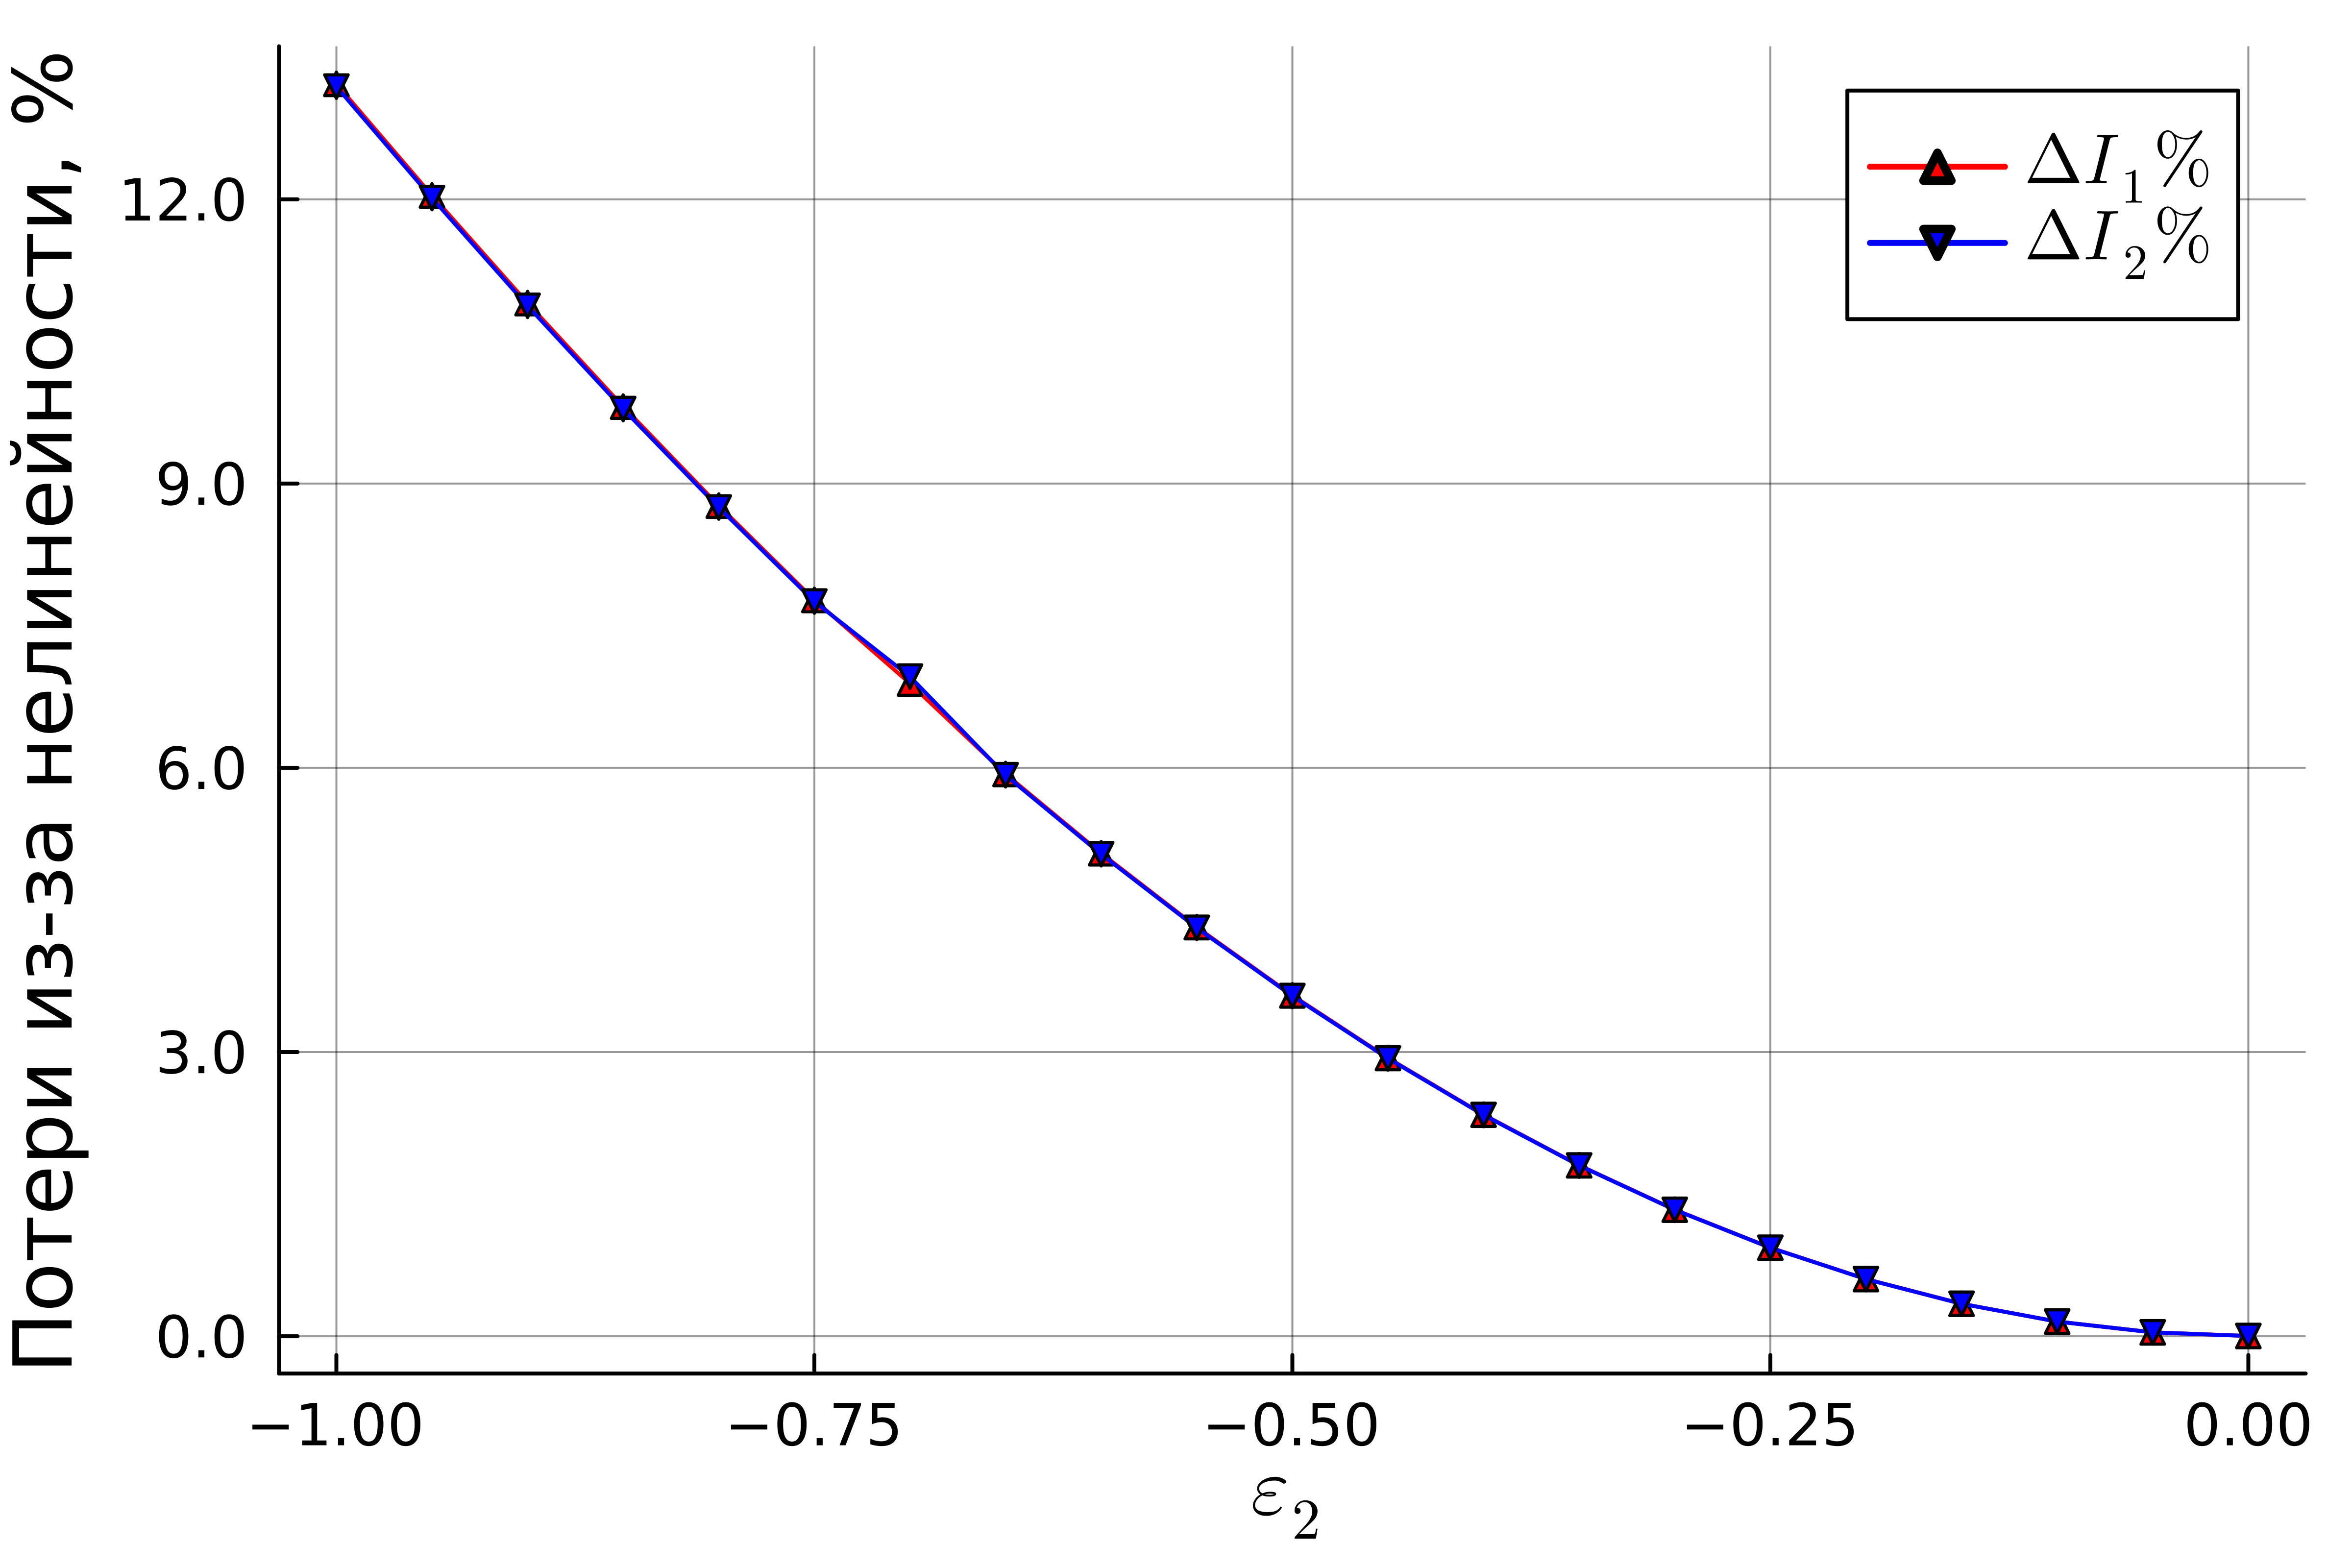
\includegraphics[width=1\linewidth]{fig72.png}
						\subcaption{Процент потерь мощности и импульса}
					\end{minipage}
					\hfill
					\begin{minipage}[h]{0.48\linewidth}
						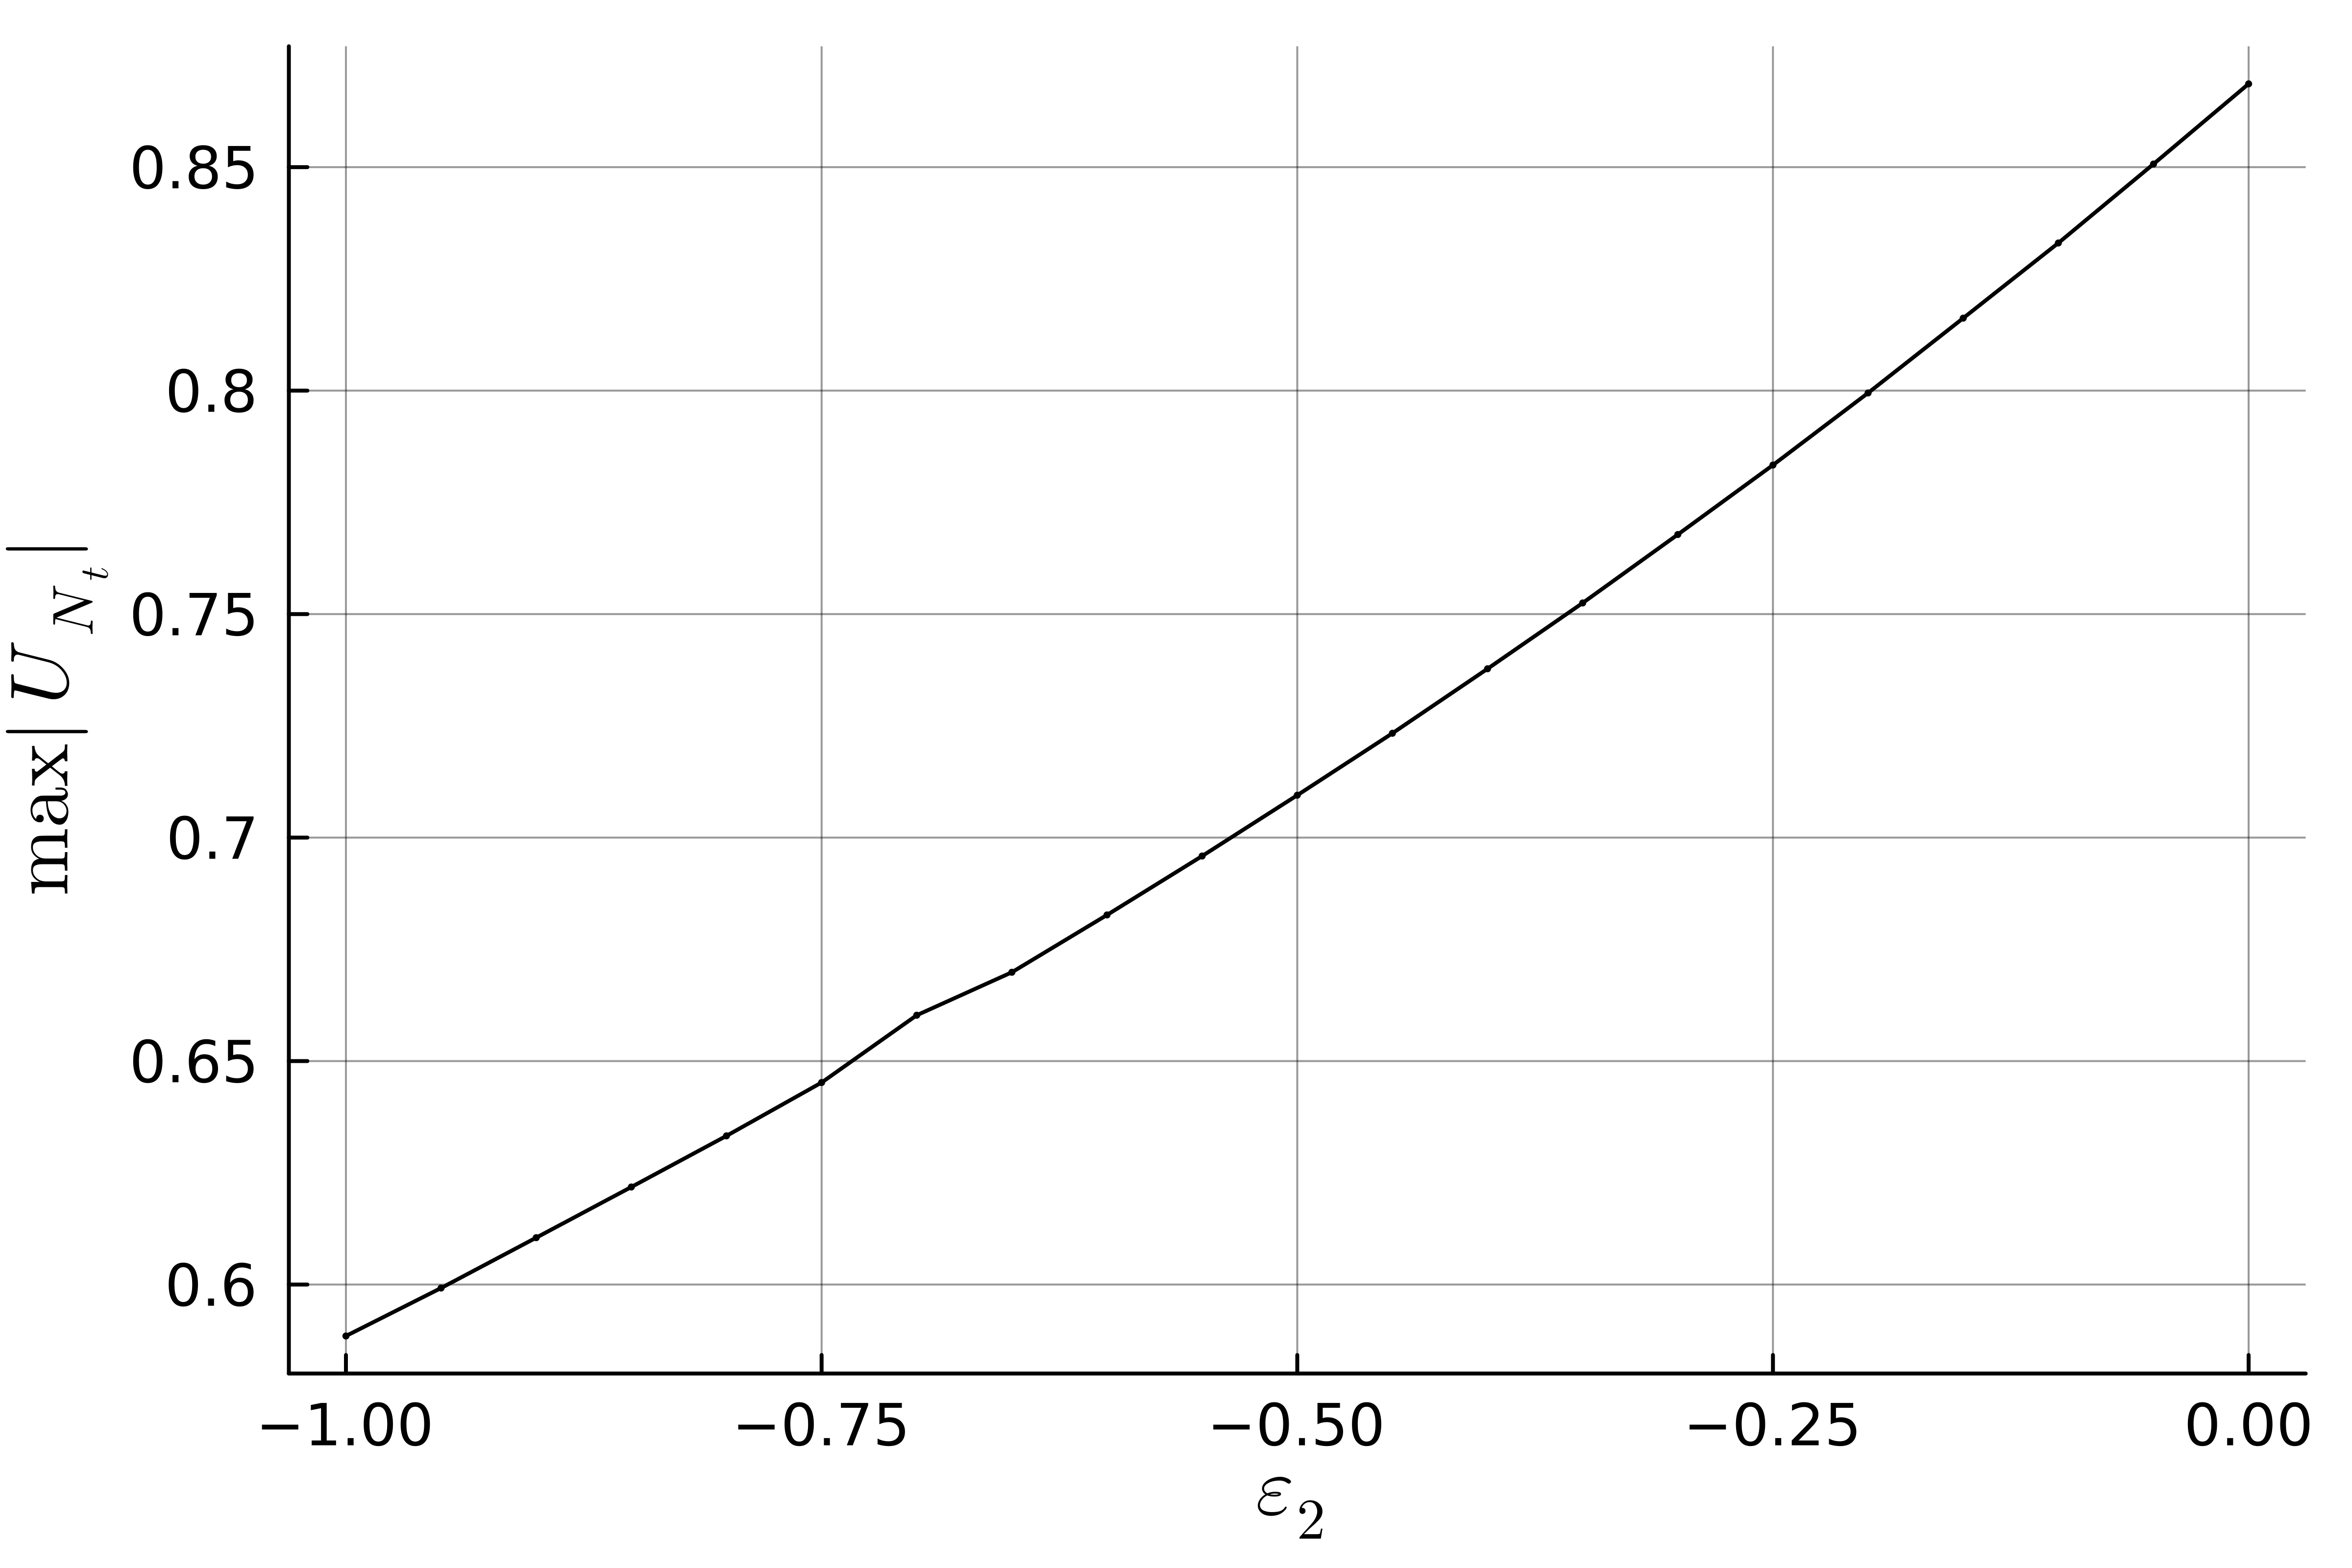
\includegraphics[width=1\linewidth]{fig73.png}
						\subcaption{Амплитуда решения в конечный момент}
					\end{minipage}
				\end{center}
				\caption{Зависимости величин относительно \(\varepsilon_{2}\) при
				\(L=160,\, T=3000,\, h=0.2,\, \tau=0.04,\)
				\(\varepsilon_{3}=0,\, \omega=0.4,\, k=0.15\).}
				\label{fig340-5_1}
			\end{figure}

			В случае \(\varepsilon_{2}>0\) обнаружены следующее наблюдения. Амплитуда результирующего импульса в начале моделирования увеличивается. Потеря солитоном импульса и мощности происходит интенсивнее и дольше, чем в случае отрицательного \(\varepsilon_{2}\), что приводит к необходимости фильтровать решение на больших временах и с большим коэффициентом \(k_{f}\). В противном случае происходит зашумление численного решения.

			Результаты моделирования для \(\varepsilon_{2}=0.5\) проиллюстрированы на Рис. \ref{fig340-5_2} и Рис. \ref{fig340-5_3}. Мощность \(I_{1}\) сохраняется с учётом диссипированной в результате фильтрации. Импульс притерпевает изменения, проиллюстрированные на Рис. \ref{fig340-5_2}. Суммарная величина \(I_{2}+I_{2f}\) не сохраняется, изменившись на \(44.8\%\). В конце моделирования при \(T=50000\) солитоном потеряно \(17.6\%\) мощности и \(18.3\%\) импульса. В конечный момент моделирования ошибка между подобранным аналитическим и численным решением составляет \(0.09\%\). Амплитуда импульса в конце моделирования колеблется, изменяясь в пределах \(0.12\%\) в зависимости от времени.

			\begin{figure}[H] %% color here
				\begin{center}
					\begin{minipage}[h]{0.48\linewidth}
						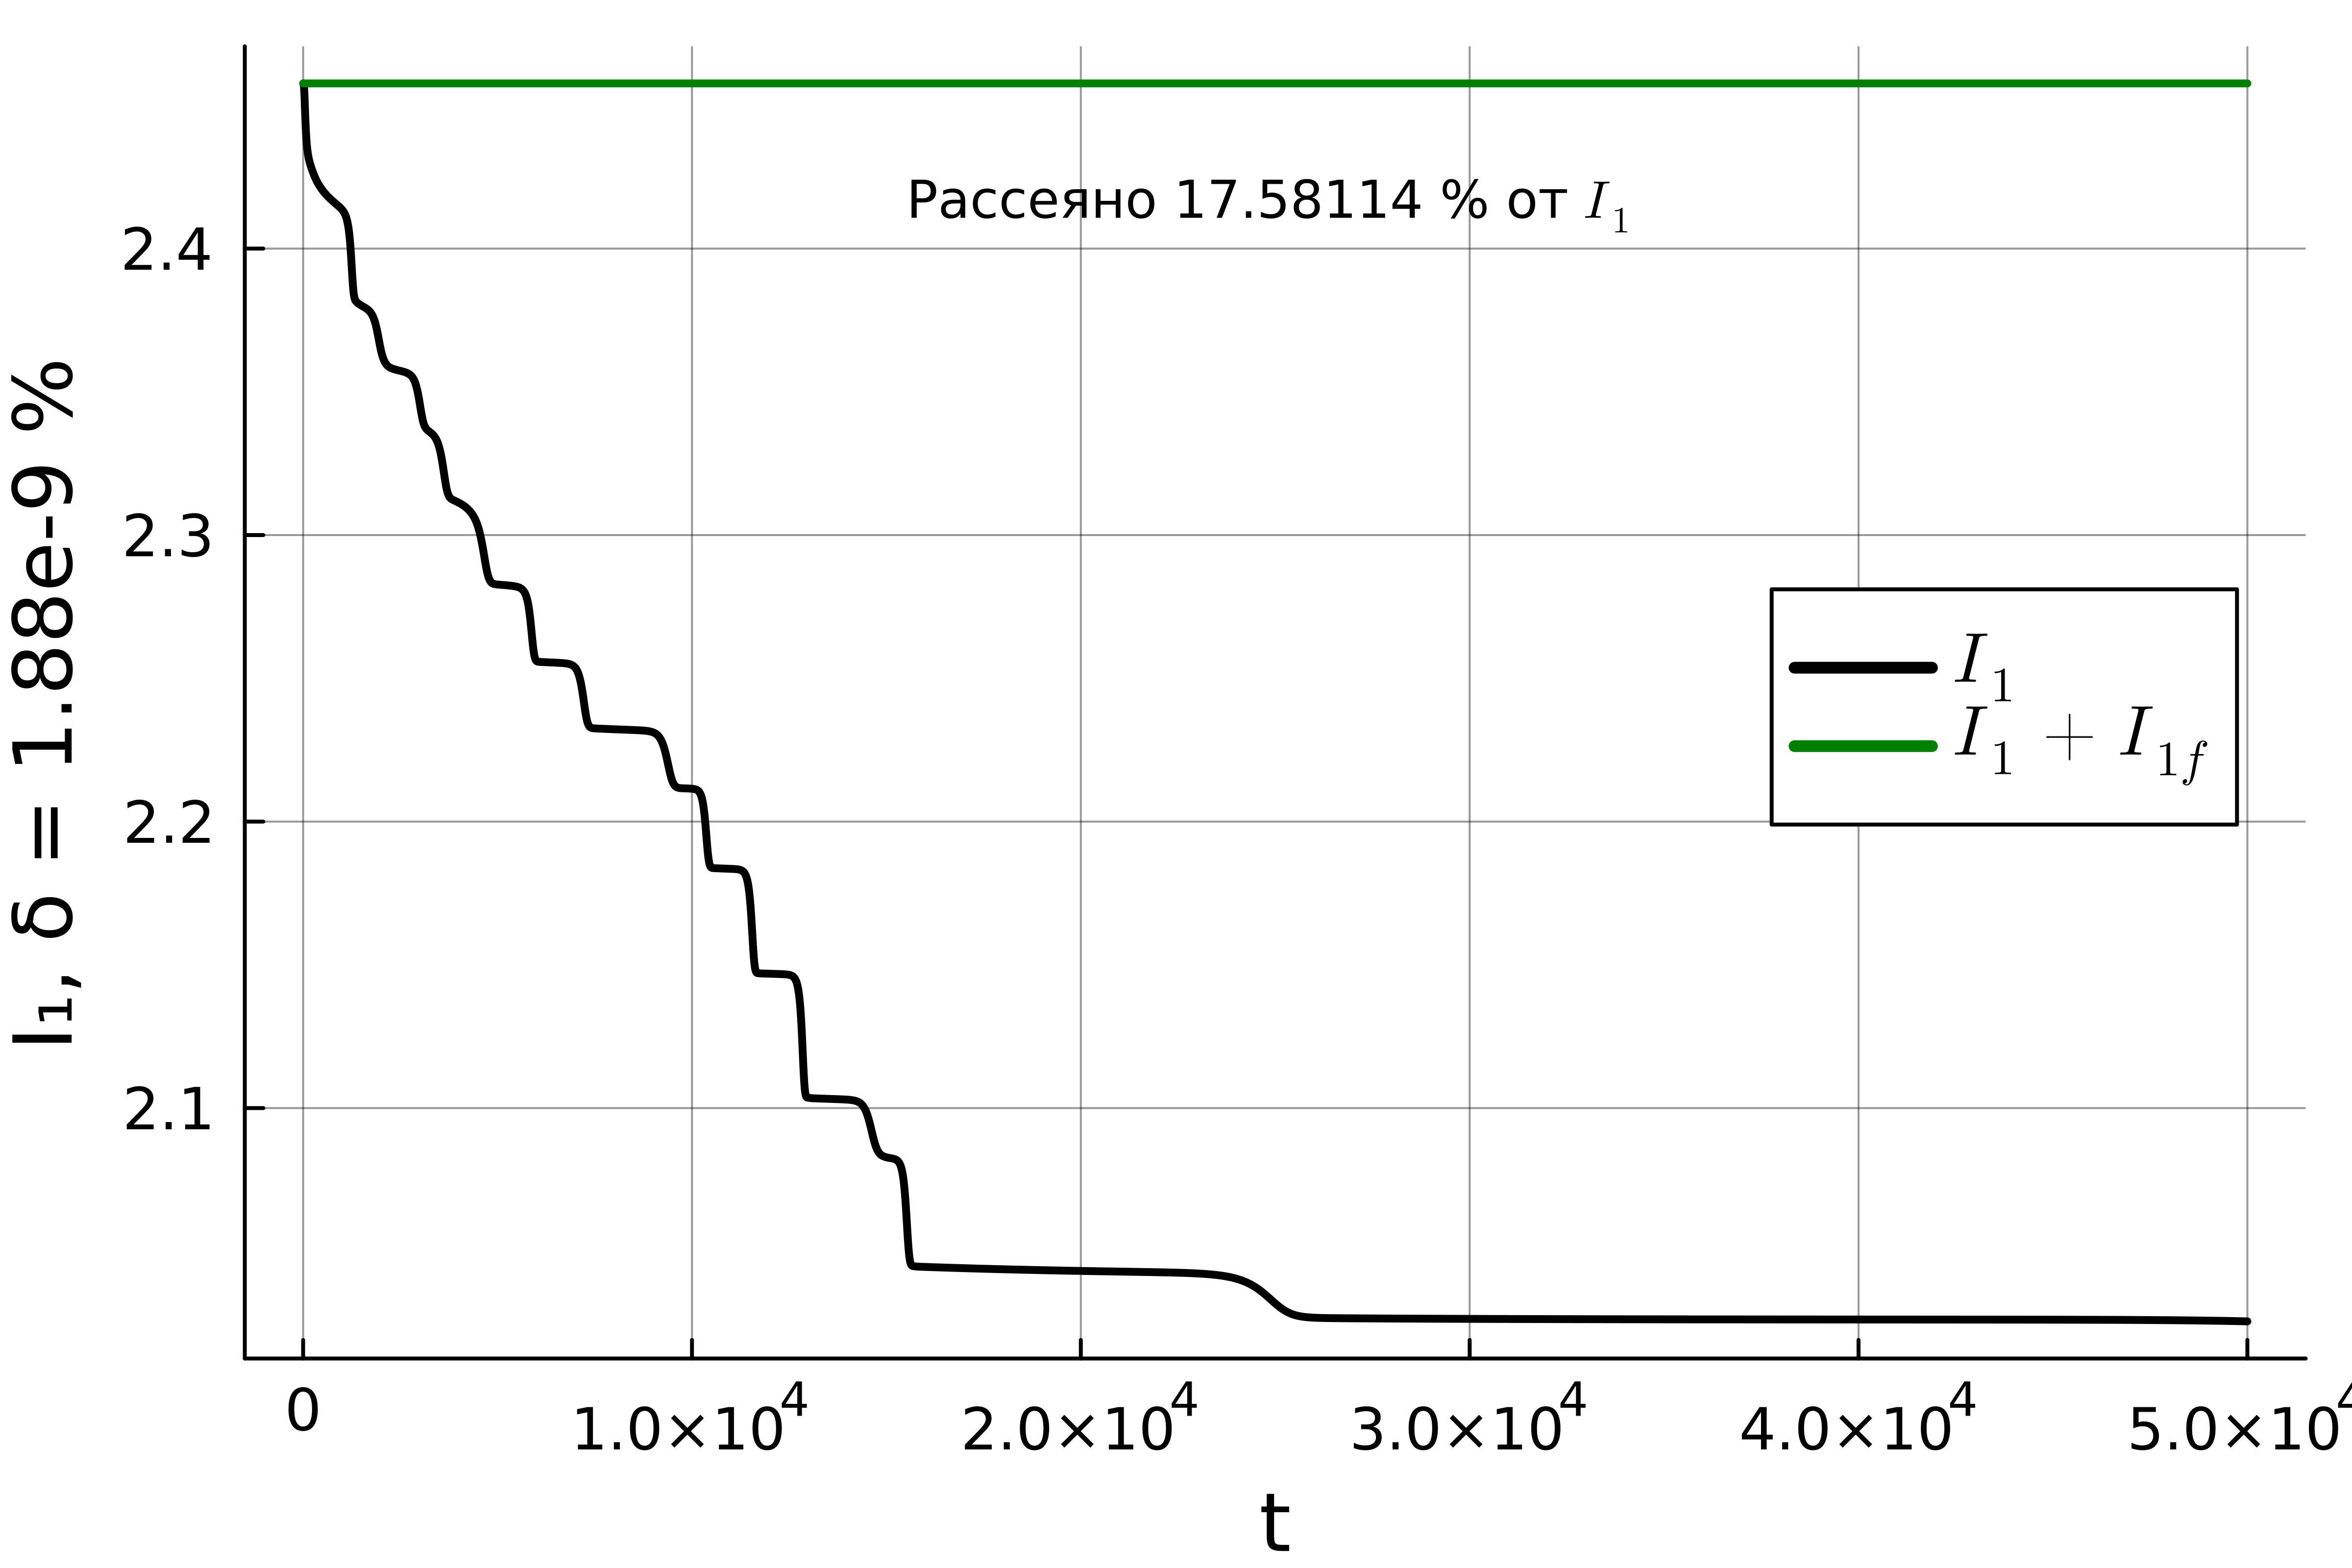
\includegraphics[width=1\linewidth]{fig74.png}
						\subcaption{Зависимость \(I_{1}\) от времени}
					\end{minipage}
					\hfill
					\begin{minipage}[h]{0.48\linewidth}
						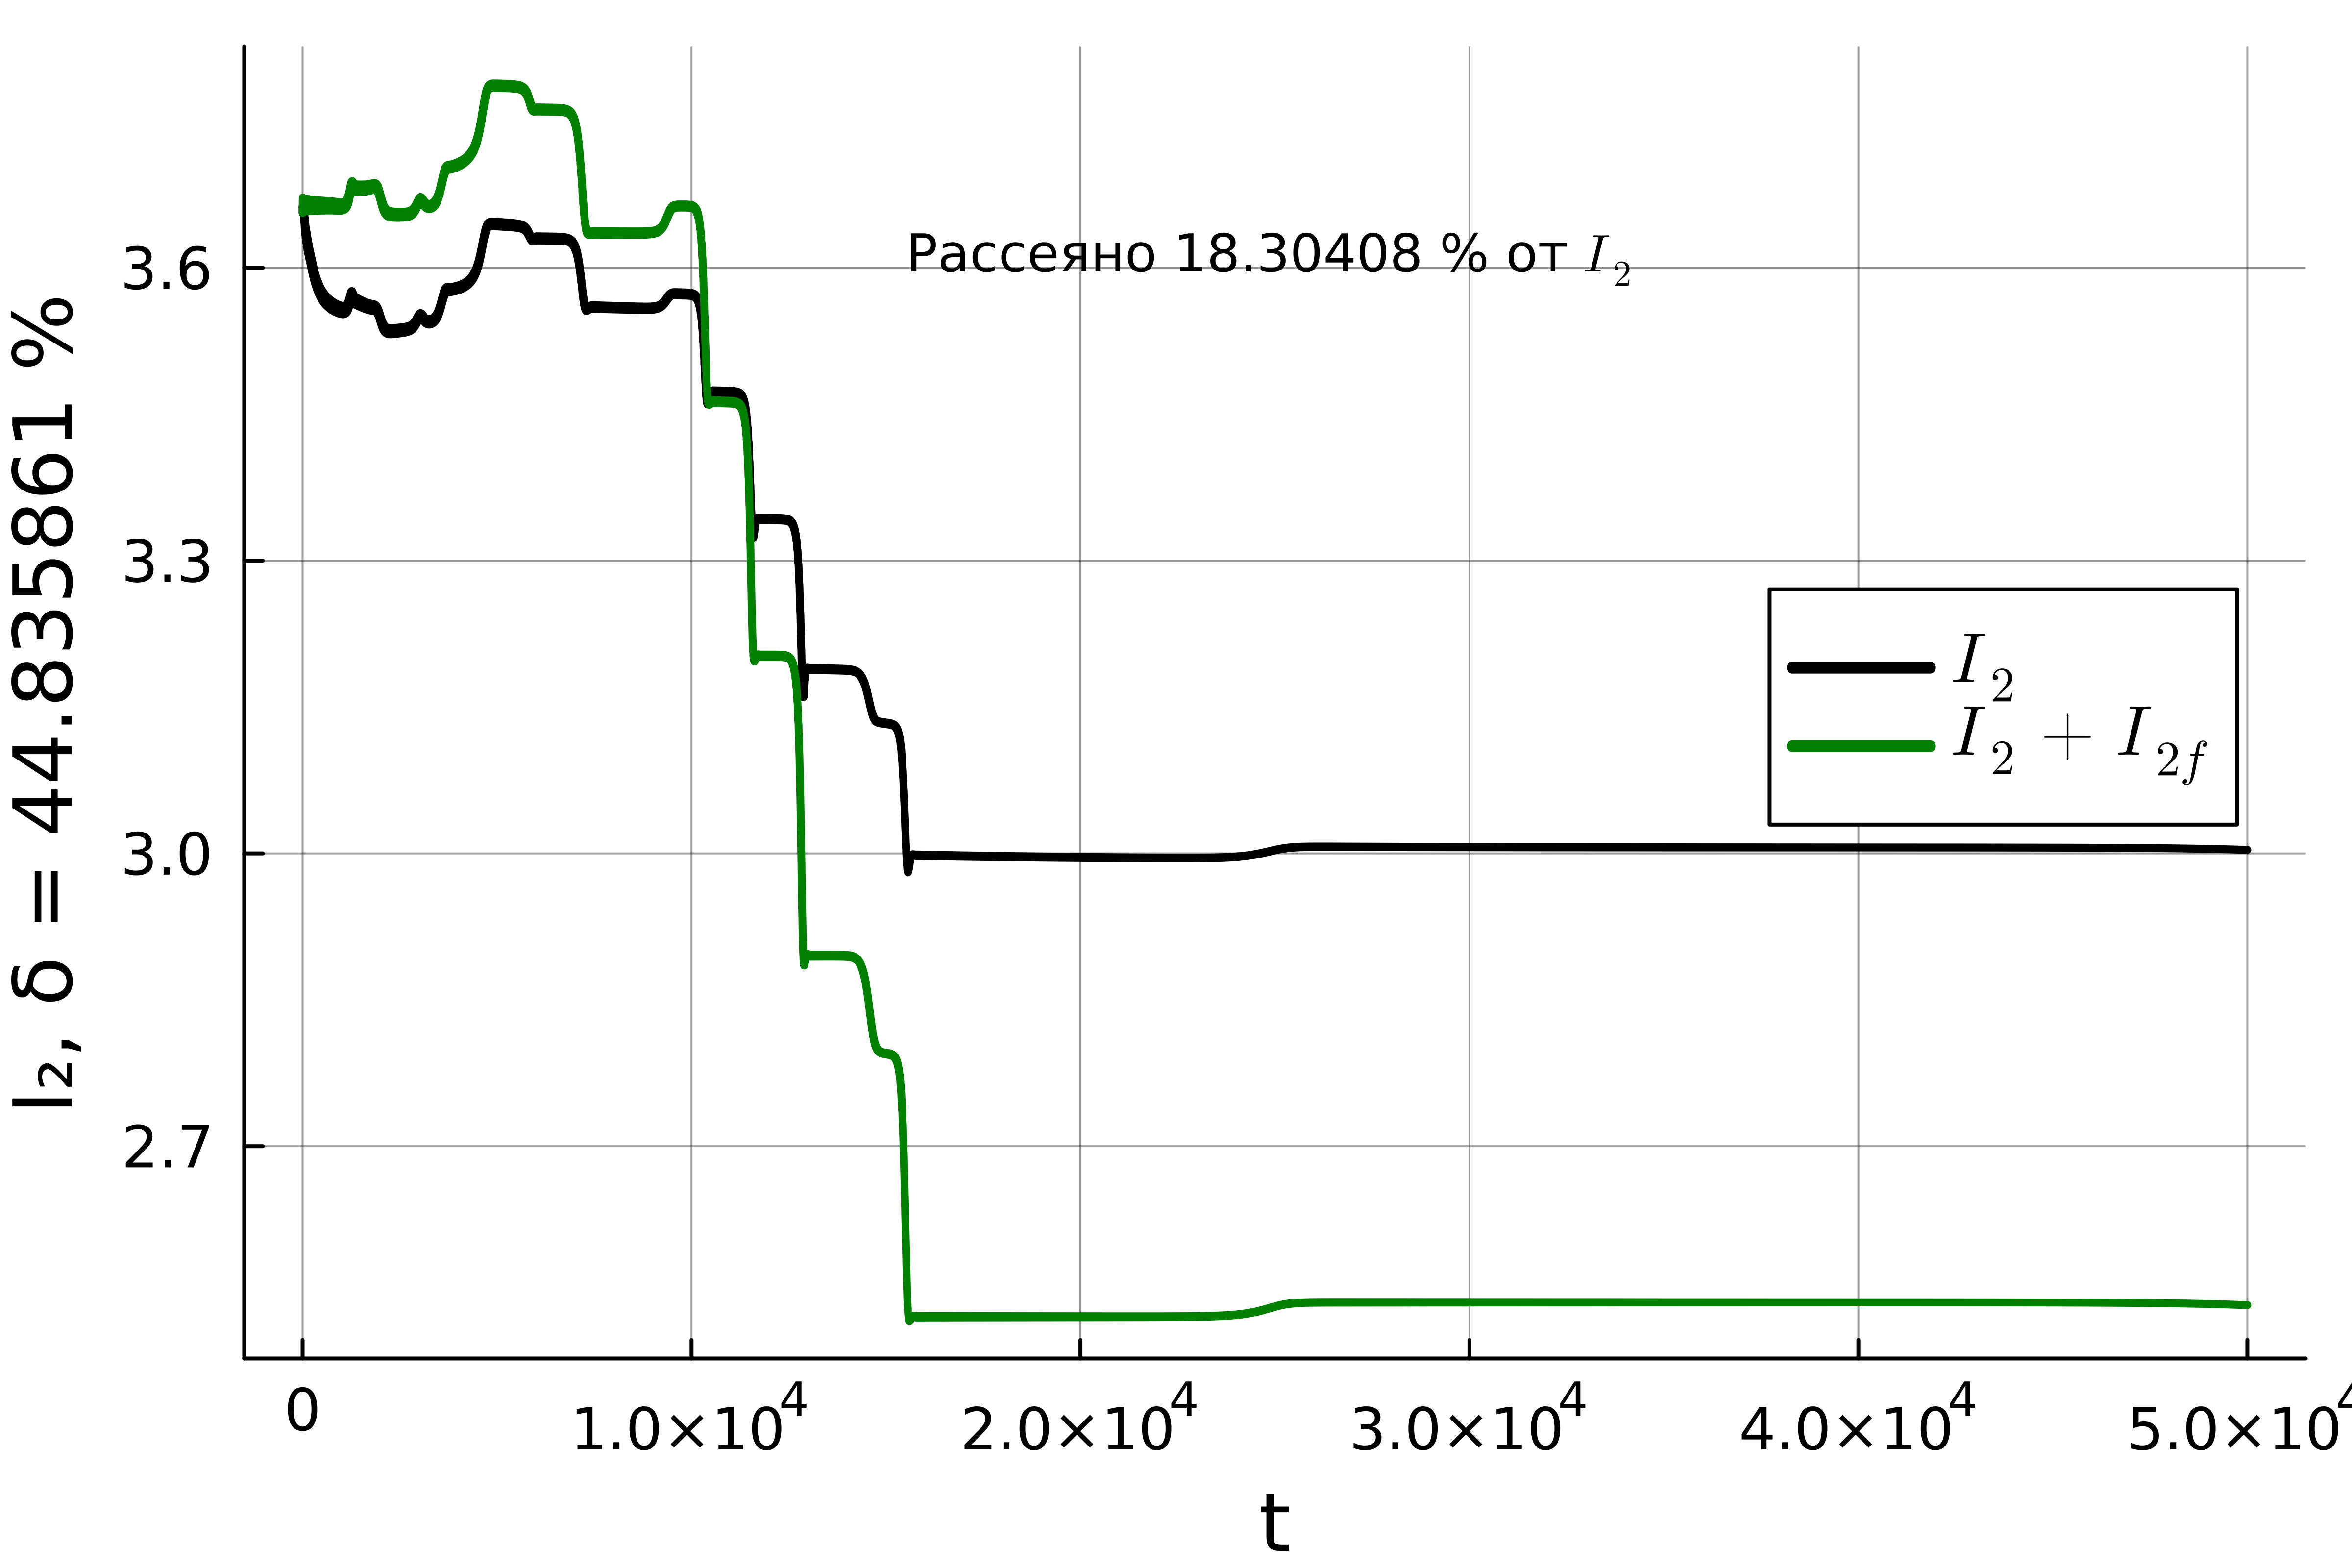
\includegraphics[width=1\linewidth]{fig75.png}
						\subcaption{Зависимость \(I_{2}\) от времени}
					\end{minipage}
				\end{center}
				\caption{Поведение законов сохранения при
				\(L=160,\, T=50000,\, h=0.2,\, \tau=0.04,\)
				\(\varepsilon_{2}=0.5,\,\varepsilon_{3}=0,\, \omega=0.4,\, k=0.15\).}
				\label{fig340-5_2}
			\end{figure}

			\begin{figure}[H] %% color here
				\begin{center}
					\begin{minipage}[h]{0.48\linewidth}
						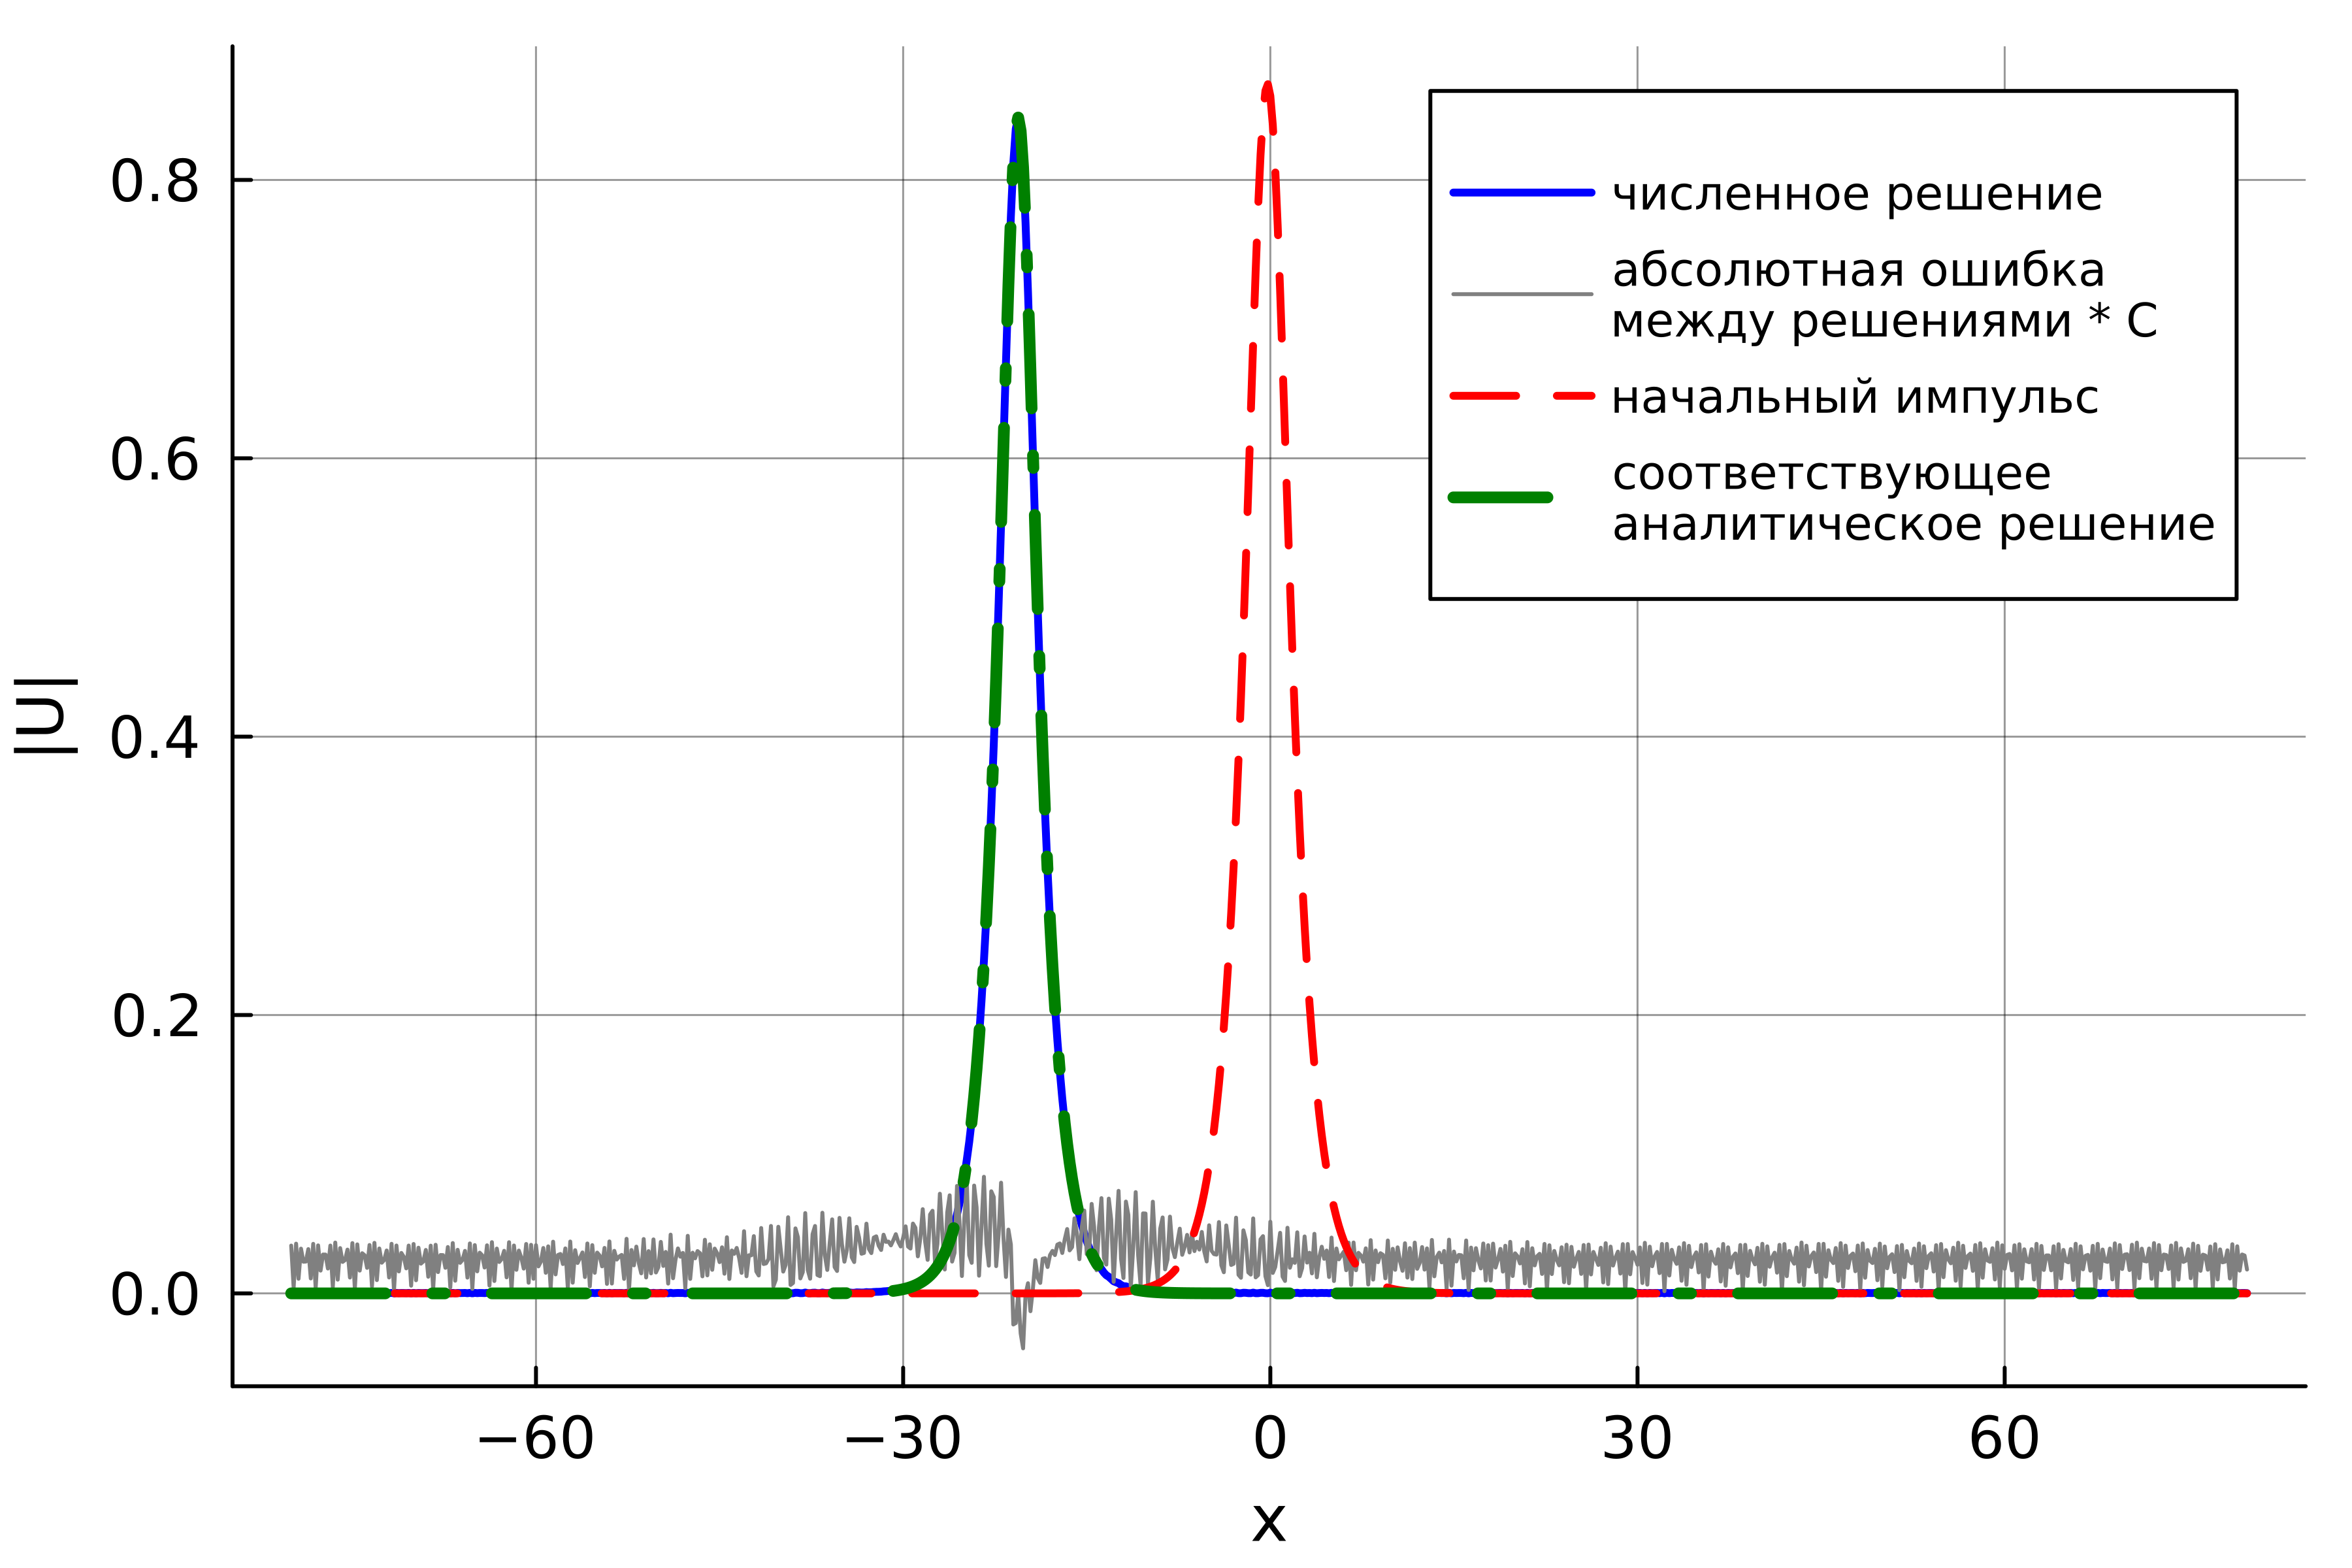
\includegraphics[width=1\linewidth]{fig76.png}
						\subcaption{Профиль решения при t=50000}
					\end{minipage}
					\hfill
					\begin{minipage}[h]{0.48\linewidth}
						\raisebox{-6.15cm}{
							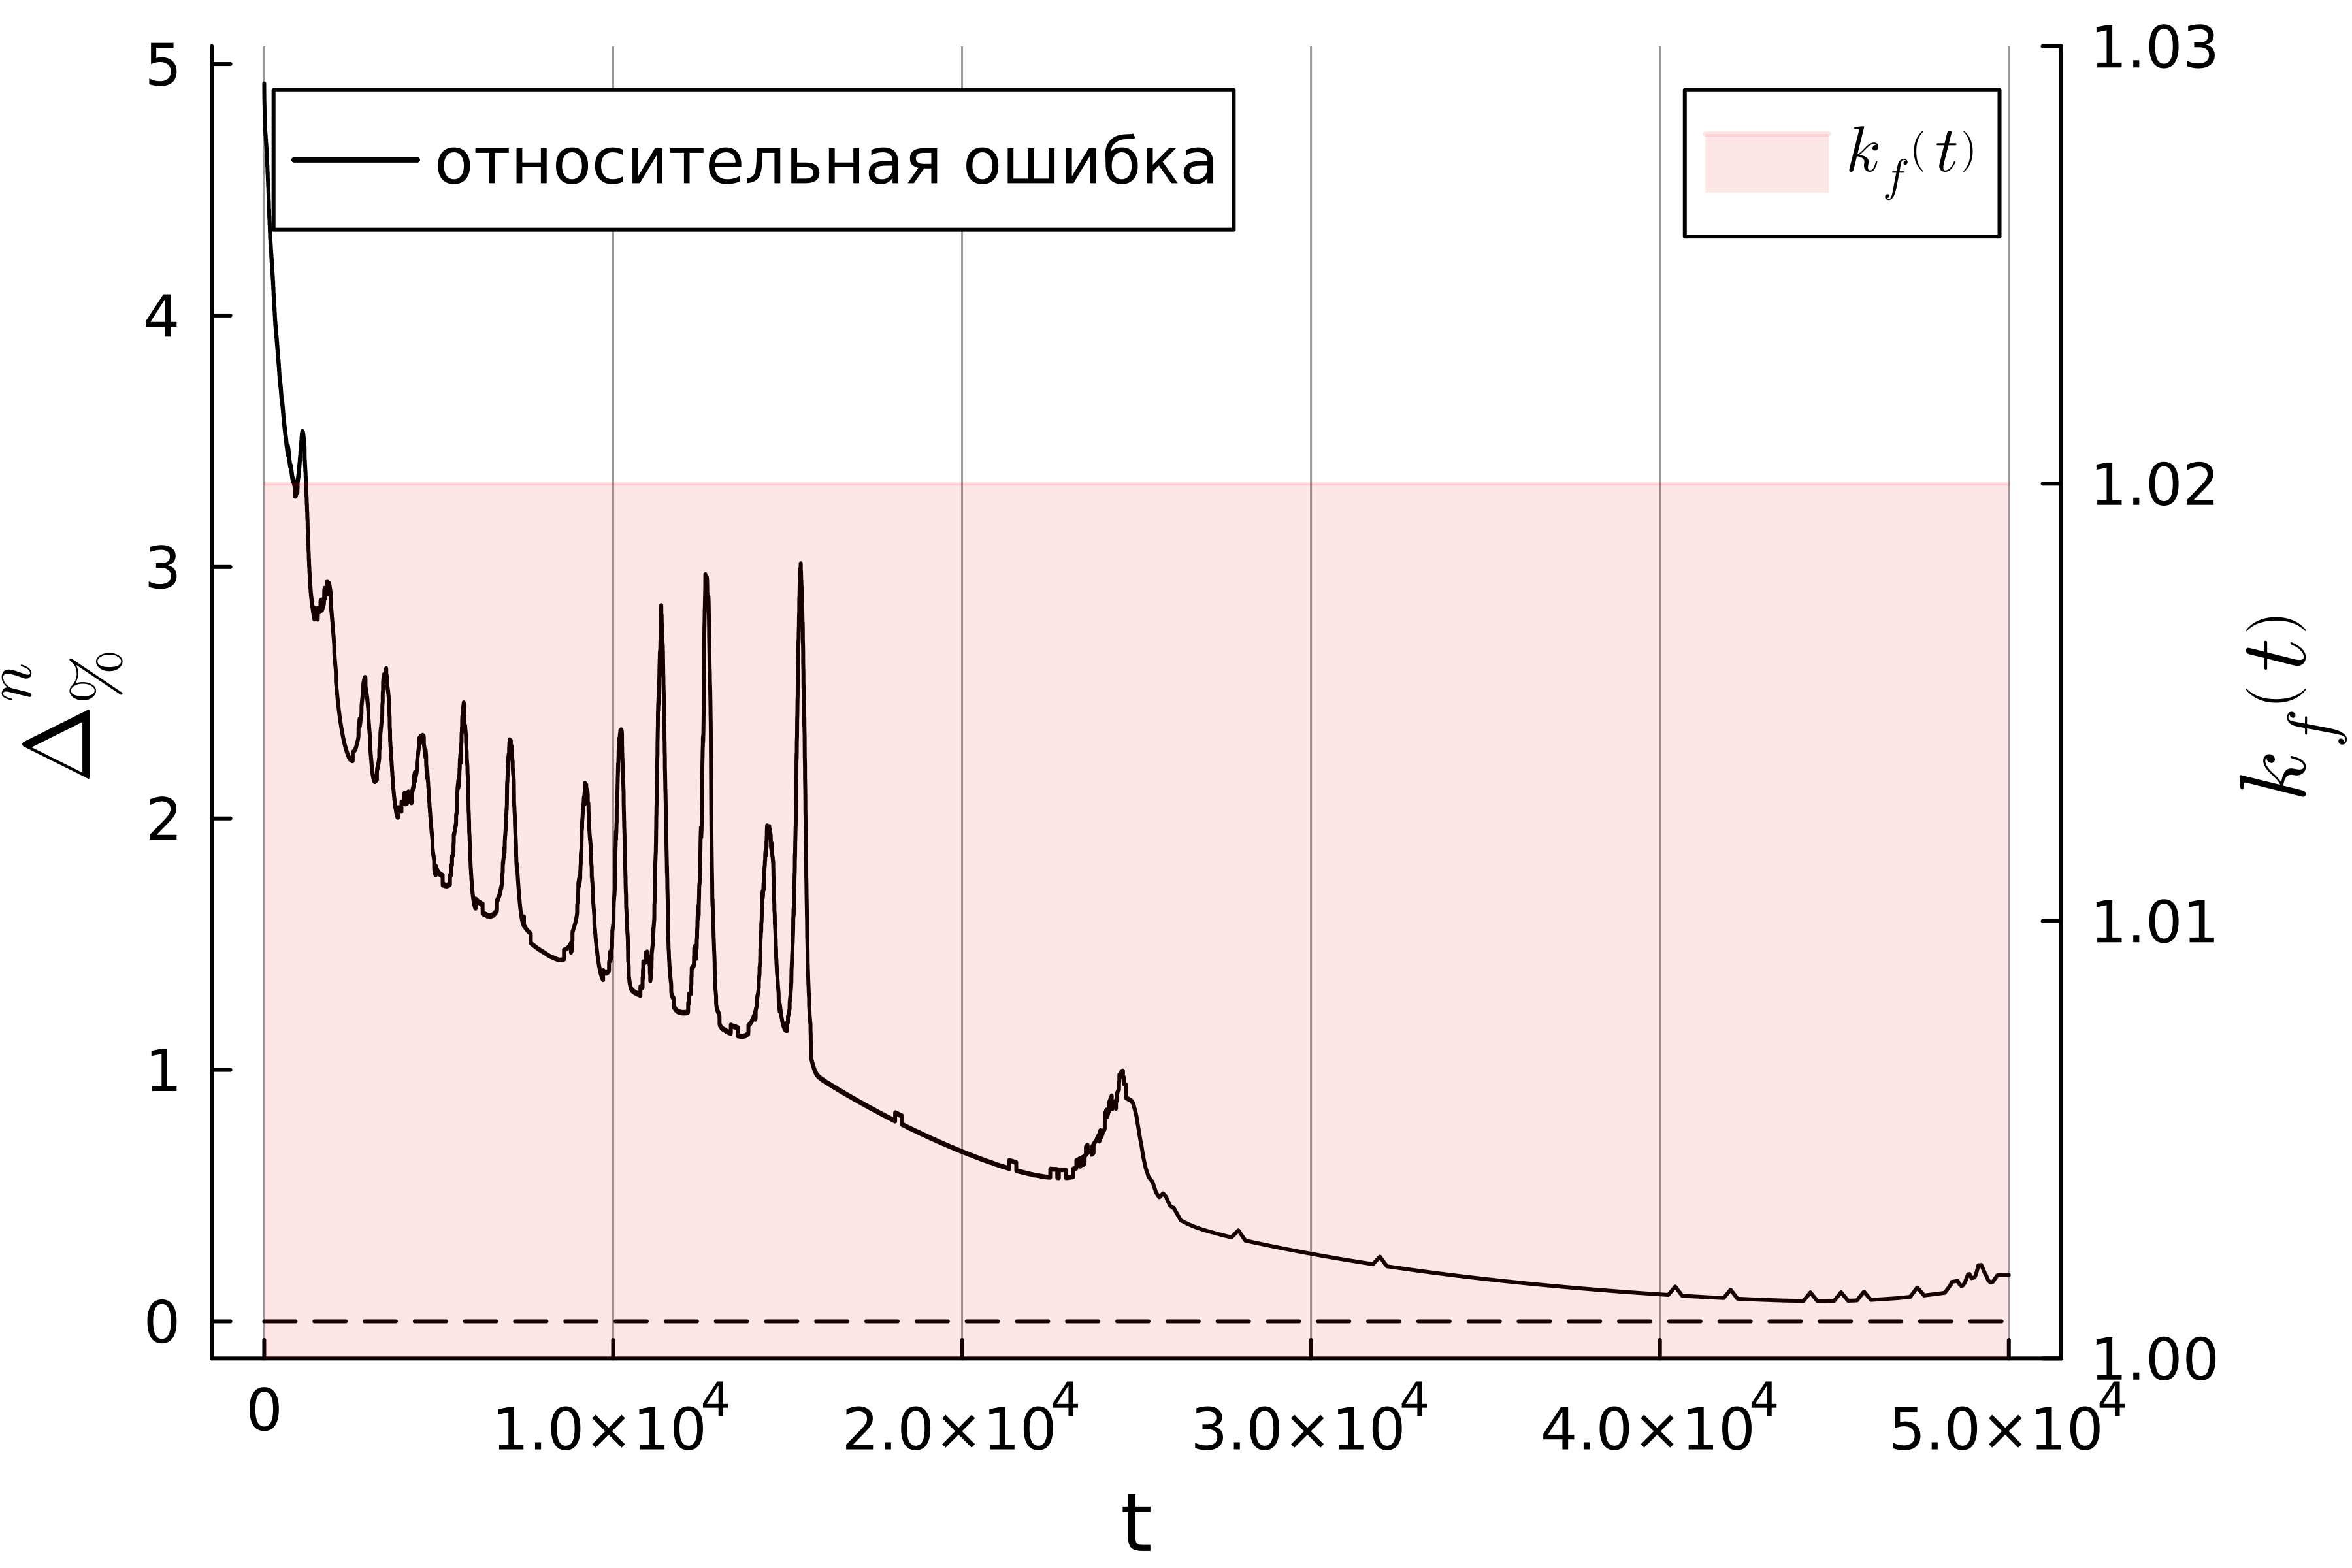
\includegraphics[width=1\linewidth]{fig77.png}
						}
						\subcaption{Зависимости относительной ошибки и коэффициента фильтрации от времени}
					\end{minipage}
				\end{center}
				\caption{Численные результаты при
				\(L=160,\, T=50000,\, h=0.2,\, \tau=0.04,\)
				\(\varepsilon_{2}=0.5,\,\varepsilon_{3}=0,\, \omega=0.4,\, k=0.15\).}
				\label{fig340-5_3}
			\end{figure}

			Учитывая приведённые результаты, о сходимости численного решения к аналитическому при \(\varepsilon_{2}>0\) рассуждать возможно, но только для достаточно малых значений параметра. Исходный солитон под воздействием степенного нелинейного члена с положительным коэффициентом притерпевает переходный процесс, который требует на порядок больше времени на установление, чем в случае \(\varepsilon_{2}<0\), и происходит с более интенсивной потерей импульса и мощности. Учитывая, что при этом закон сохранения импульса не выполняется, моделирование процесса распространения уединённой волны в рамках модели с \(\varepsilon_{2}>0\) в общем случае не имеет физического смысла, однако полезно для понимания влияния нелинейных членов в уравнении модели.

			В качестве дополнительного аргумента в пользу нефизичности моделирований процессов распространения импульса при \(\varepsilon_{2}>0\) приведём зависимости конечной амплитуды импульса и его потерь в зависимости от \(\varepsilon_{2}>0\). Результаты проиллюстрированы на Рис. \ref{fig340-5-4}. Зависимость перестаёт быть регулярной. Также при моделированиях начинает нарушатся сеточная сходимость.

			\begin{figure}[H] %% color here
				\begin{center}
					\begin{minipage}[h]{0.48\linewidth}
						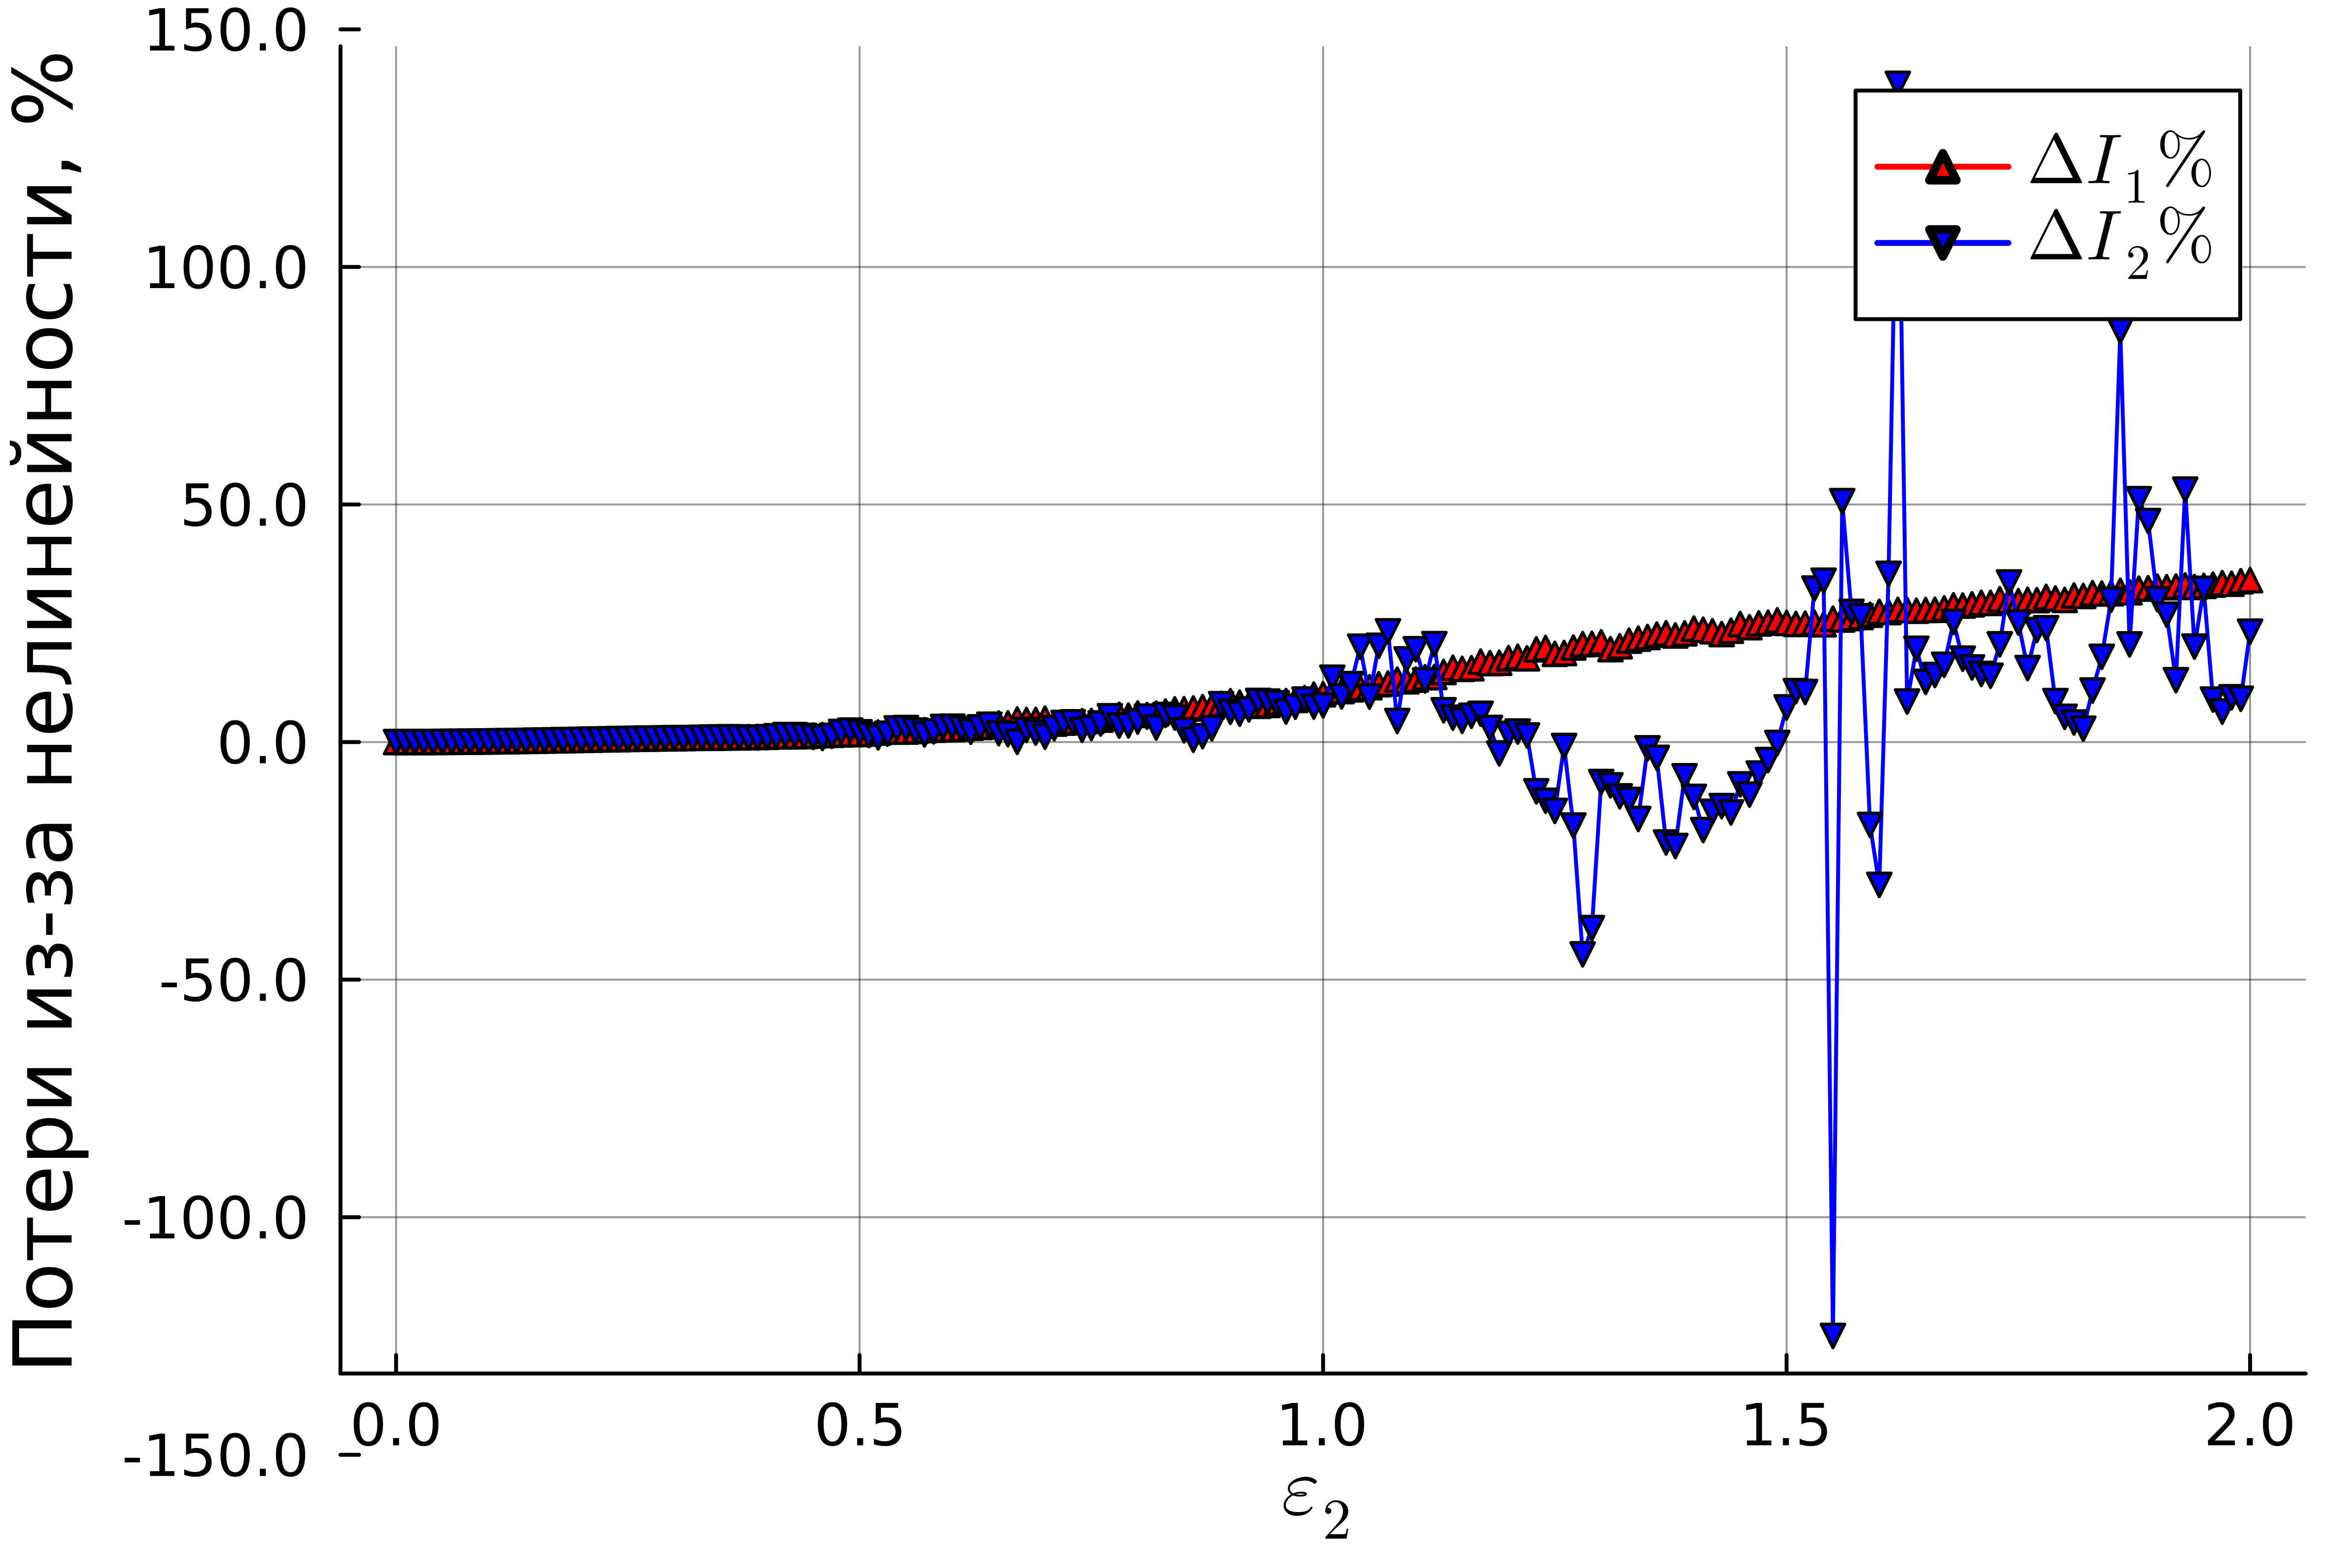
\includegraphics[width=1\linewidth]{fig78.png}
						\subcaption{Процент потерь мощности и импульса}
					\end{minipage}
					\hfill
					\begin{minipage}[h]{0.48\linewidth}
						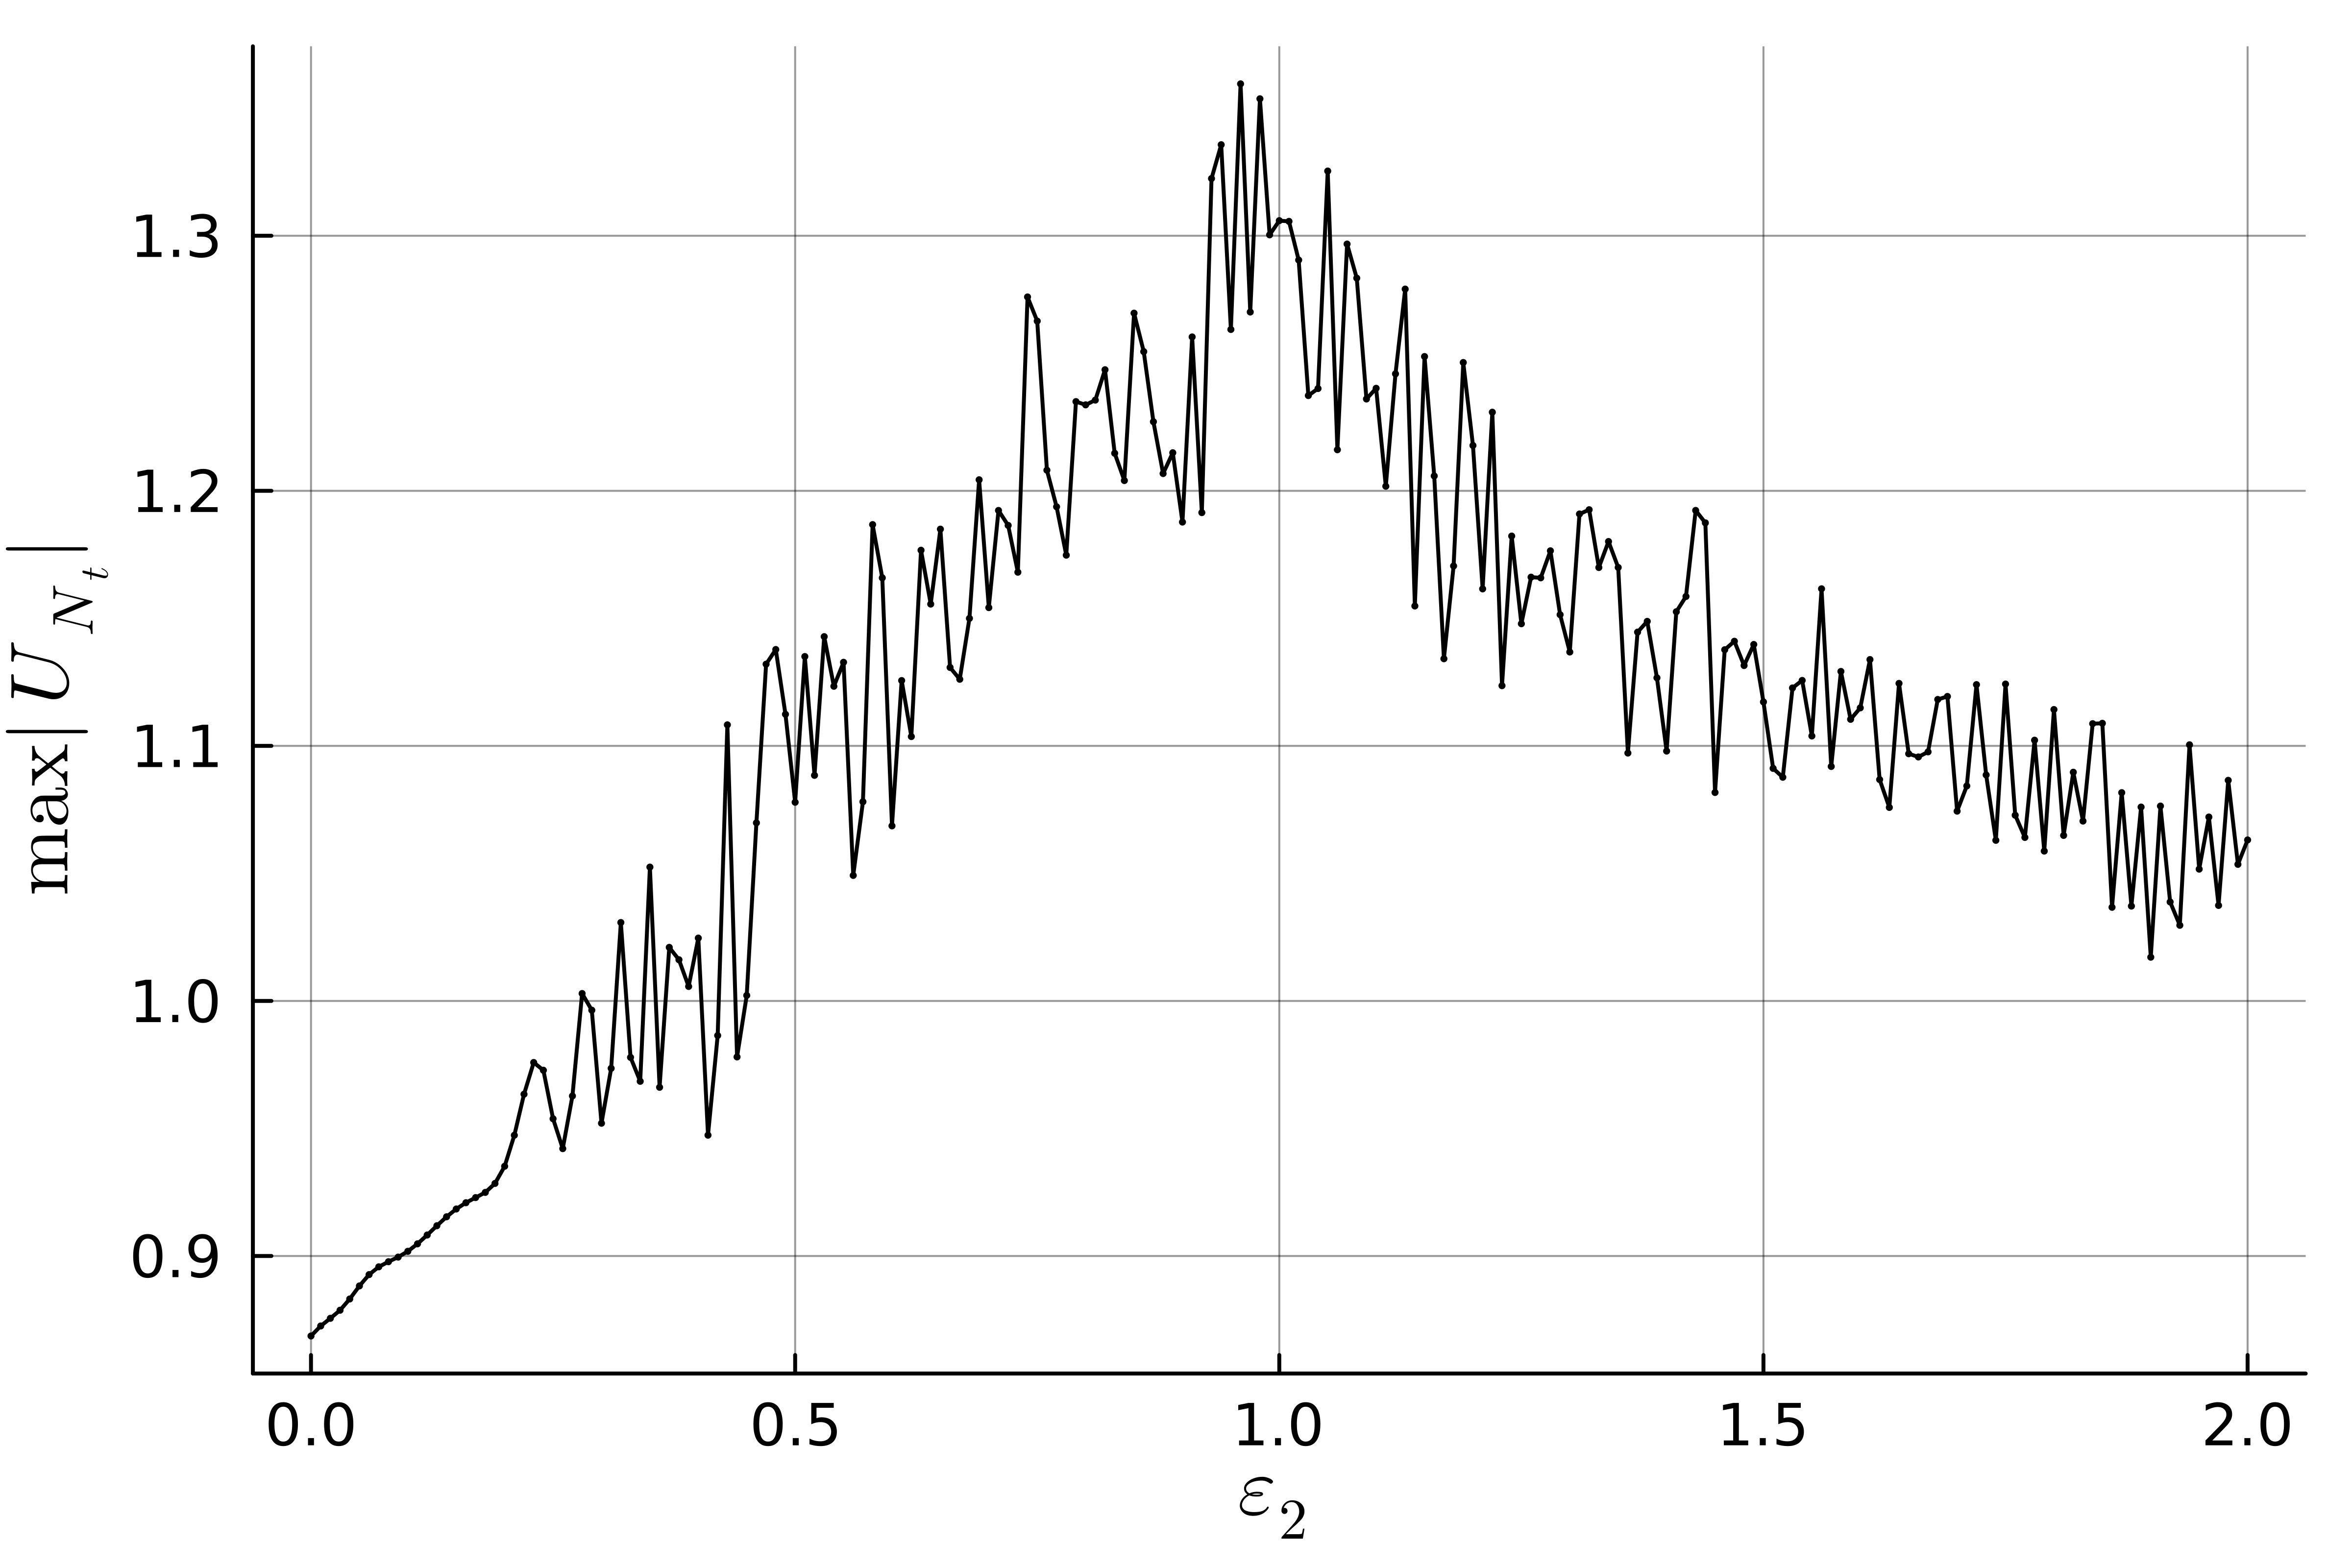
\includegraphics[width=1\linewidth]{fig79.png}
						\subcaption{Амплитуда решения в конечный момент}
					\end{minipage}
				\end{center}
				\caption{Зависимости величин относительно \(\varepsilon_{2}\) при
				\(L=160,\, T=1000,\, h=0.2,\, \tau=0.04,\)
				\(\varepsilon_{3}=0,\, \omega=0.4,\, k=0.15\).}
				\label{fig340-5_4}
			\end{figure}

			Рассмотрим более общий характер нелинейностей в модели при \(\varepsilon_{3}\ne0\). Отметим, что аналитическое решение (\ref{eq24}), построенное в разделе \ref{ch210} существует только для положительных \(\varepsilon_{2}\) и \(\varepsilon_{3}\) в силу ограничений и соотношений, использованных при его выводе. Более того, аналитическое решение существует только для тех \(\varepsilon_{2}\) и \(\varepsilon_{3}\), по которым возможно найти параметры \(M_{0}\) и \(M_{1}\) из соотношений (\ref{eq19}). В противном случае построить по данным параметрам нелинейности соответствующее аналитическое решение не получится. Проверим, возможен ли переход исходного импульса (\ref{eq48}) под действием положительных параметров \(\varepsilon_{2}\) и \(\varepsilon_{3}\) к построенному решению (\ref{eq24}). На Рис. \ref{fig340-6} проиллюстрированы профили решения в различные моменты времени.
			\begin{figure}[H] %% color here
				\begin{center}
					\begin{minipage}[h]{0.48\linewidth}
						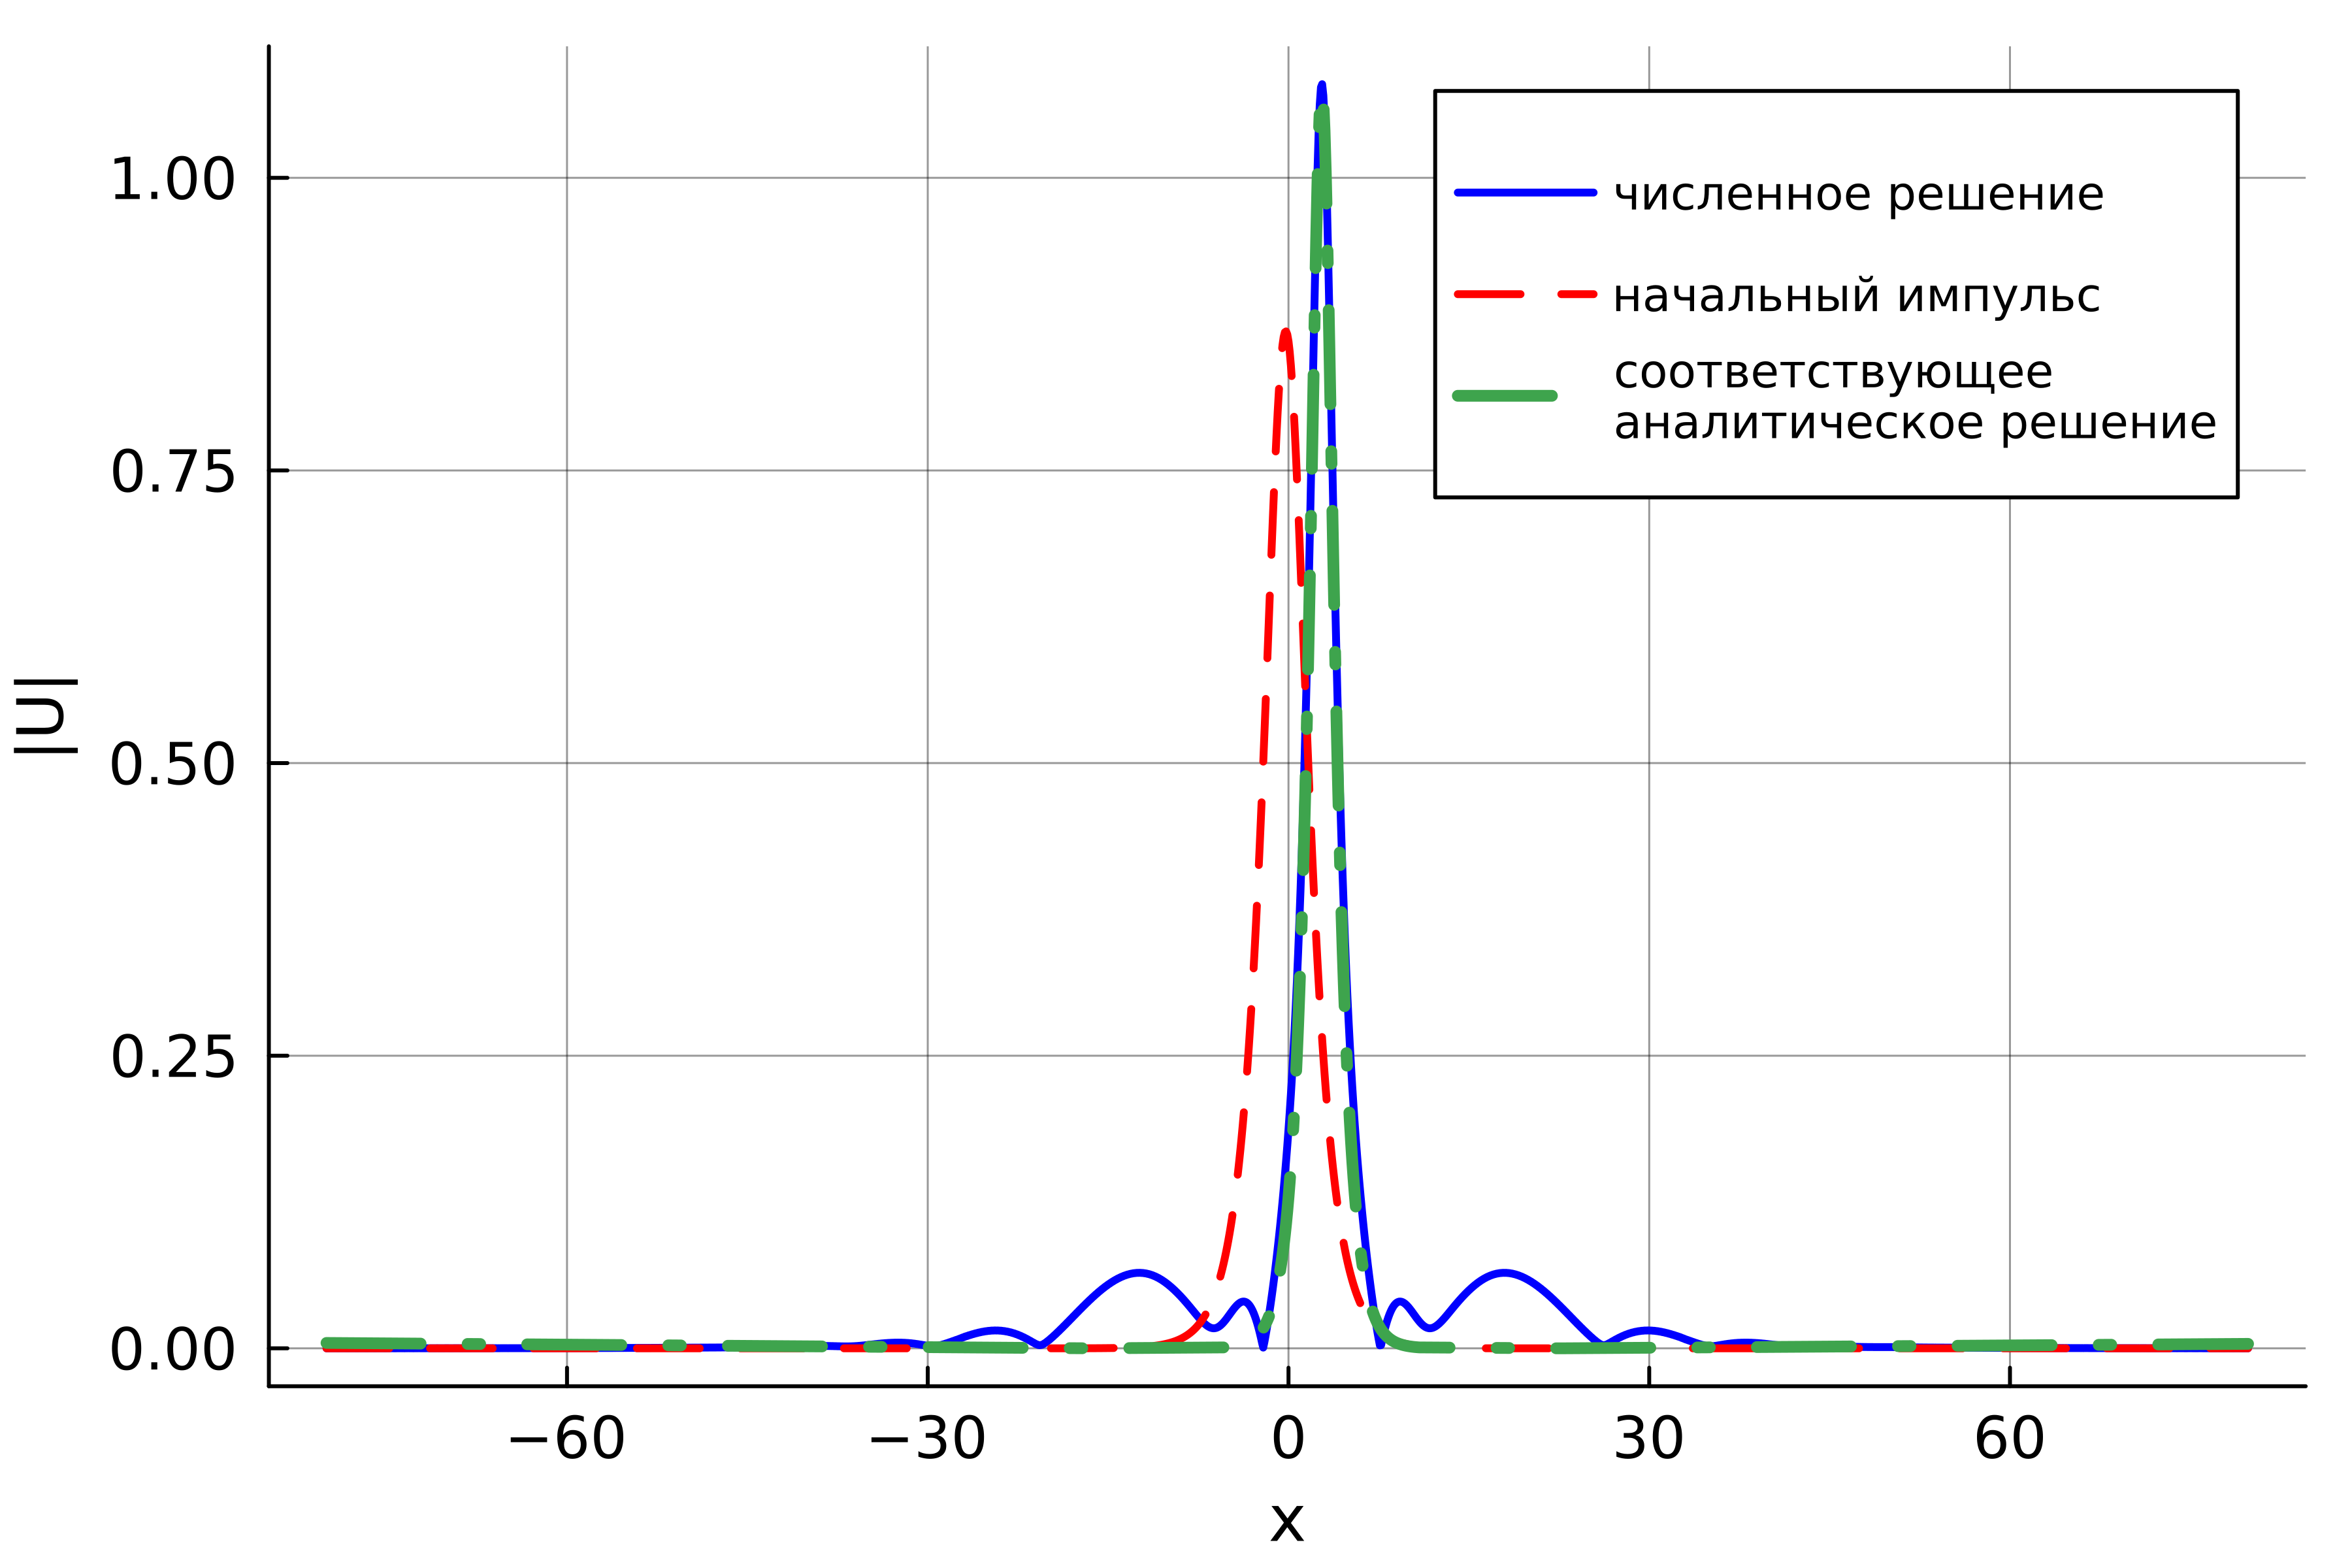
\includegraphics[width=1\linewidth]{fig67.png}
						\subcaption{Профиль решения при t=10}
					\end{minipage}
					\hfill
					\begin{minipage}[h]{0.48\linewidth}
						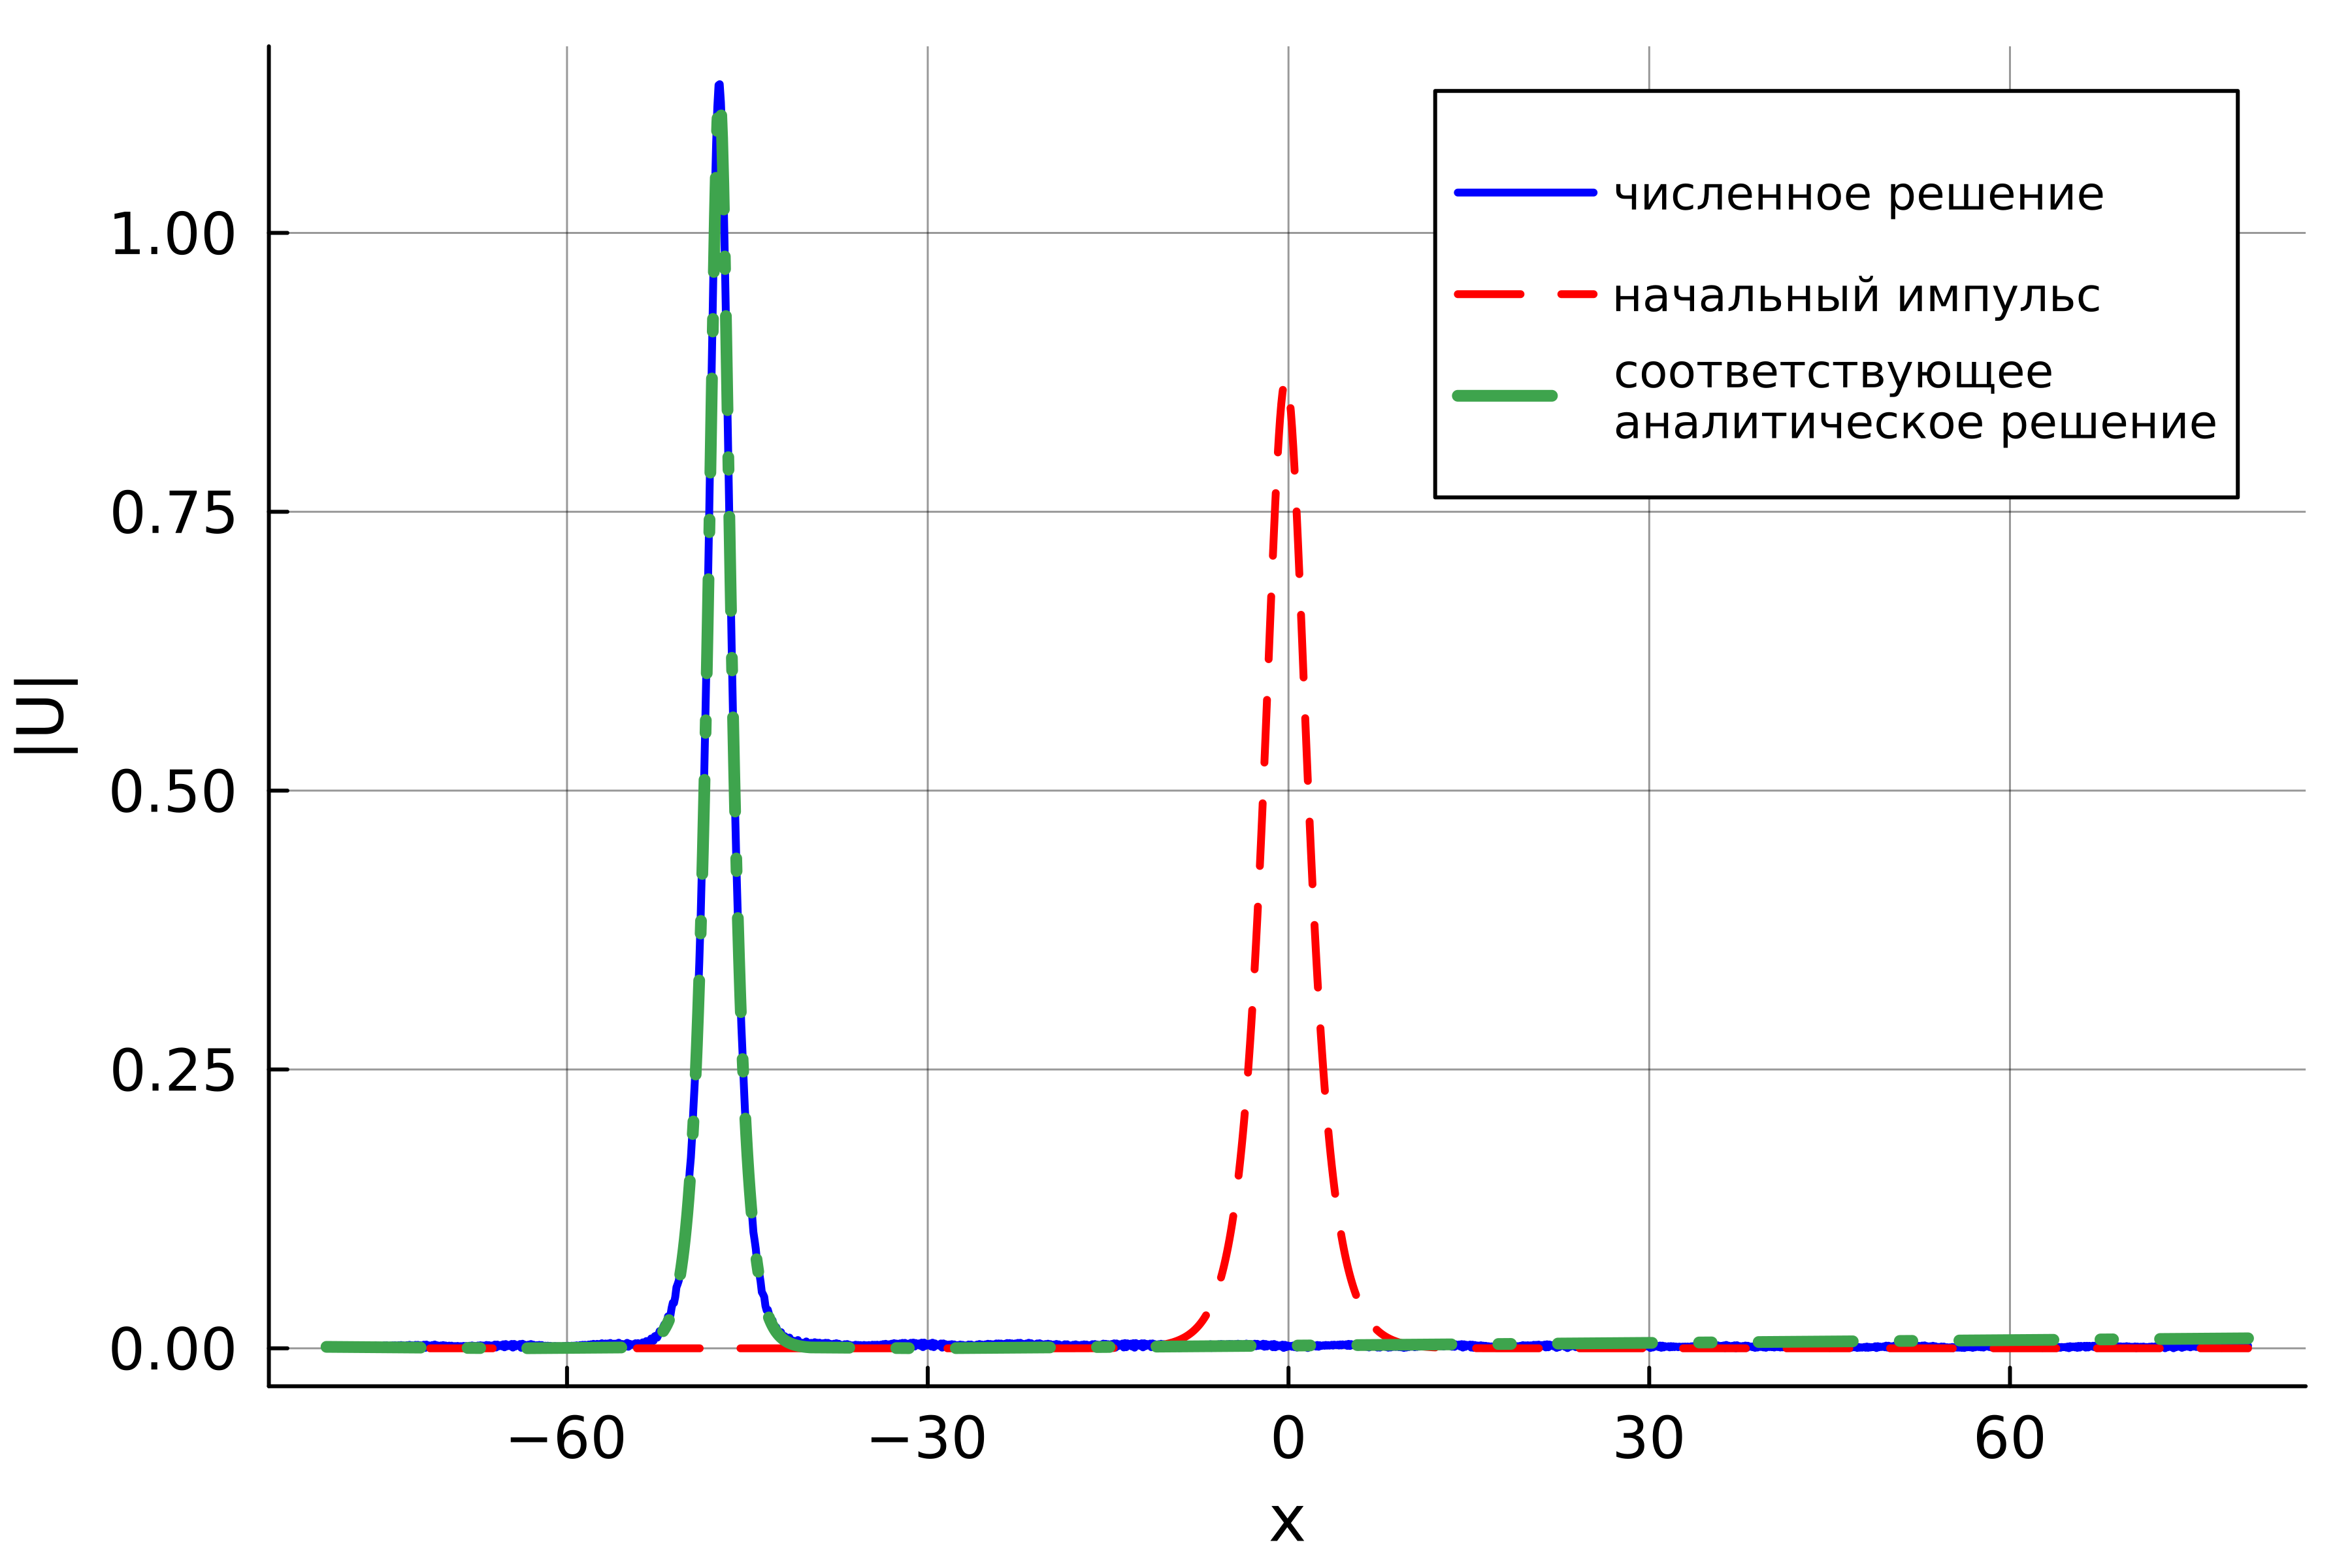
\includegraphics[width=1\linewidth]{fig68.png}
						\subcaption{Профиль решения при t=50000}
					\end{minipage}
				\end{center}
				\caption{Численные результаты распространения импульса (\ref{eq55}) при
				\(L=160,\, T=50000,\, h=0.2,\, \tau=0.04,\)
				\(\varepsilon_{2}=0.65,\,\varepsilon_{3}=0.08,\, \omega=0.4,\, k=0.15\).}
				\label{fig340-6}
			\end{figure}

			На Рис. \ref{fig340-7} проиллюстрировано поведение законов сохранения для моделирования. Результаты аналогичны моделированию, проведённому для \(\varepsilon_{2}=0.5\) и \(\varepsilon_{3}=0\). Закон сохранения импульса не выполняется. В конце моделирования по численному решению подобран солитон вида (\ref{eq24}) с относительной разницей, равной \(0.107\%\).
			\begin{figure}[H] %% color here
				\begin{center}
					\begin{minipage}[h]{0.48\linewidth}
						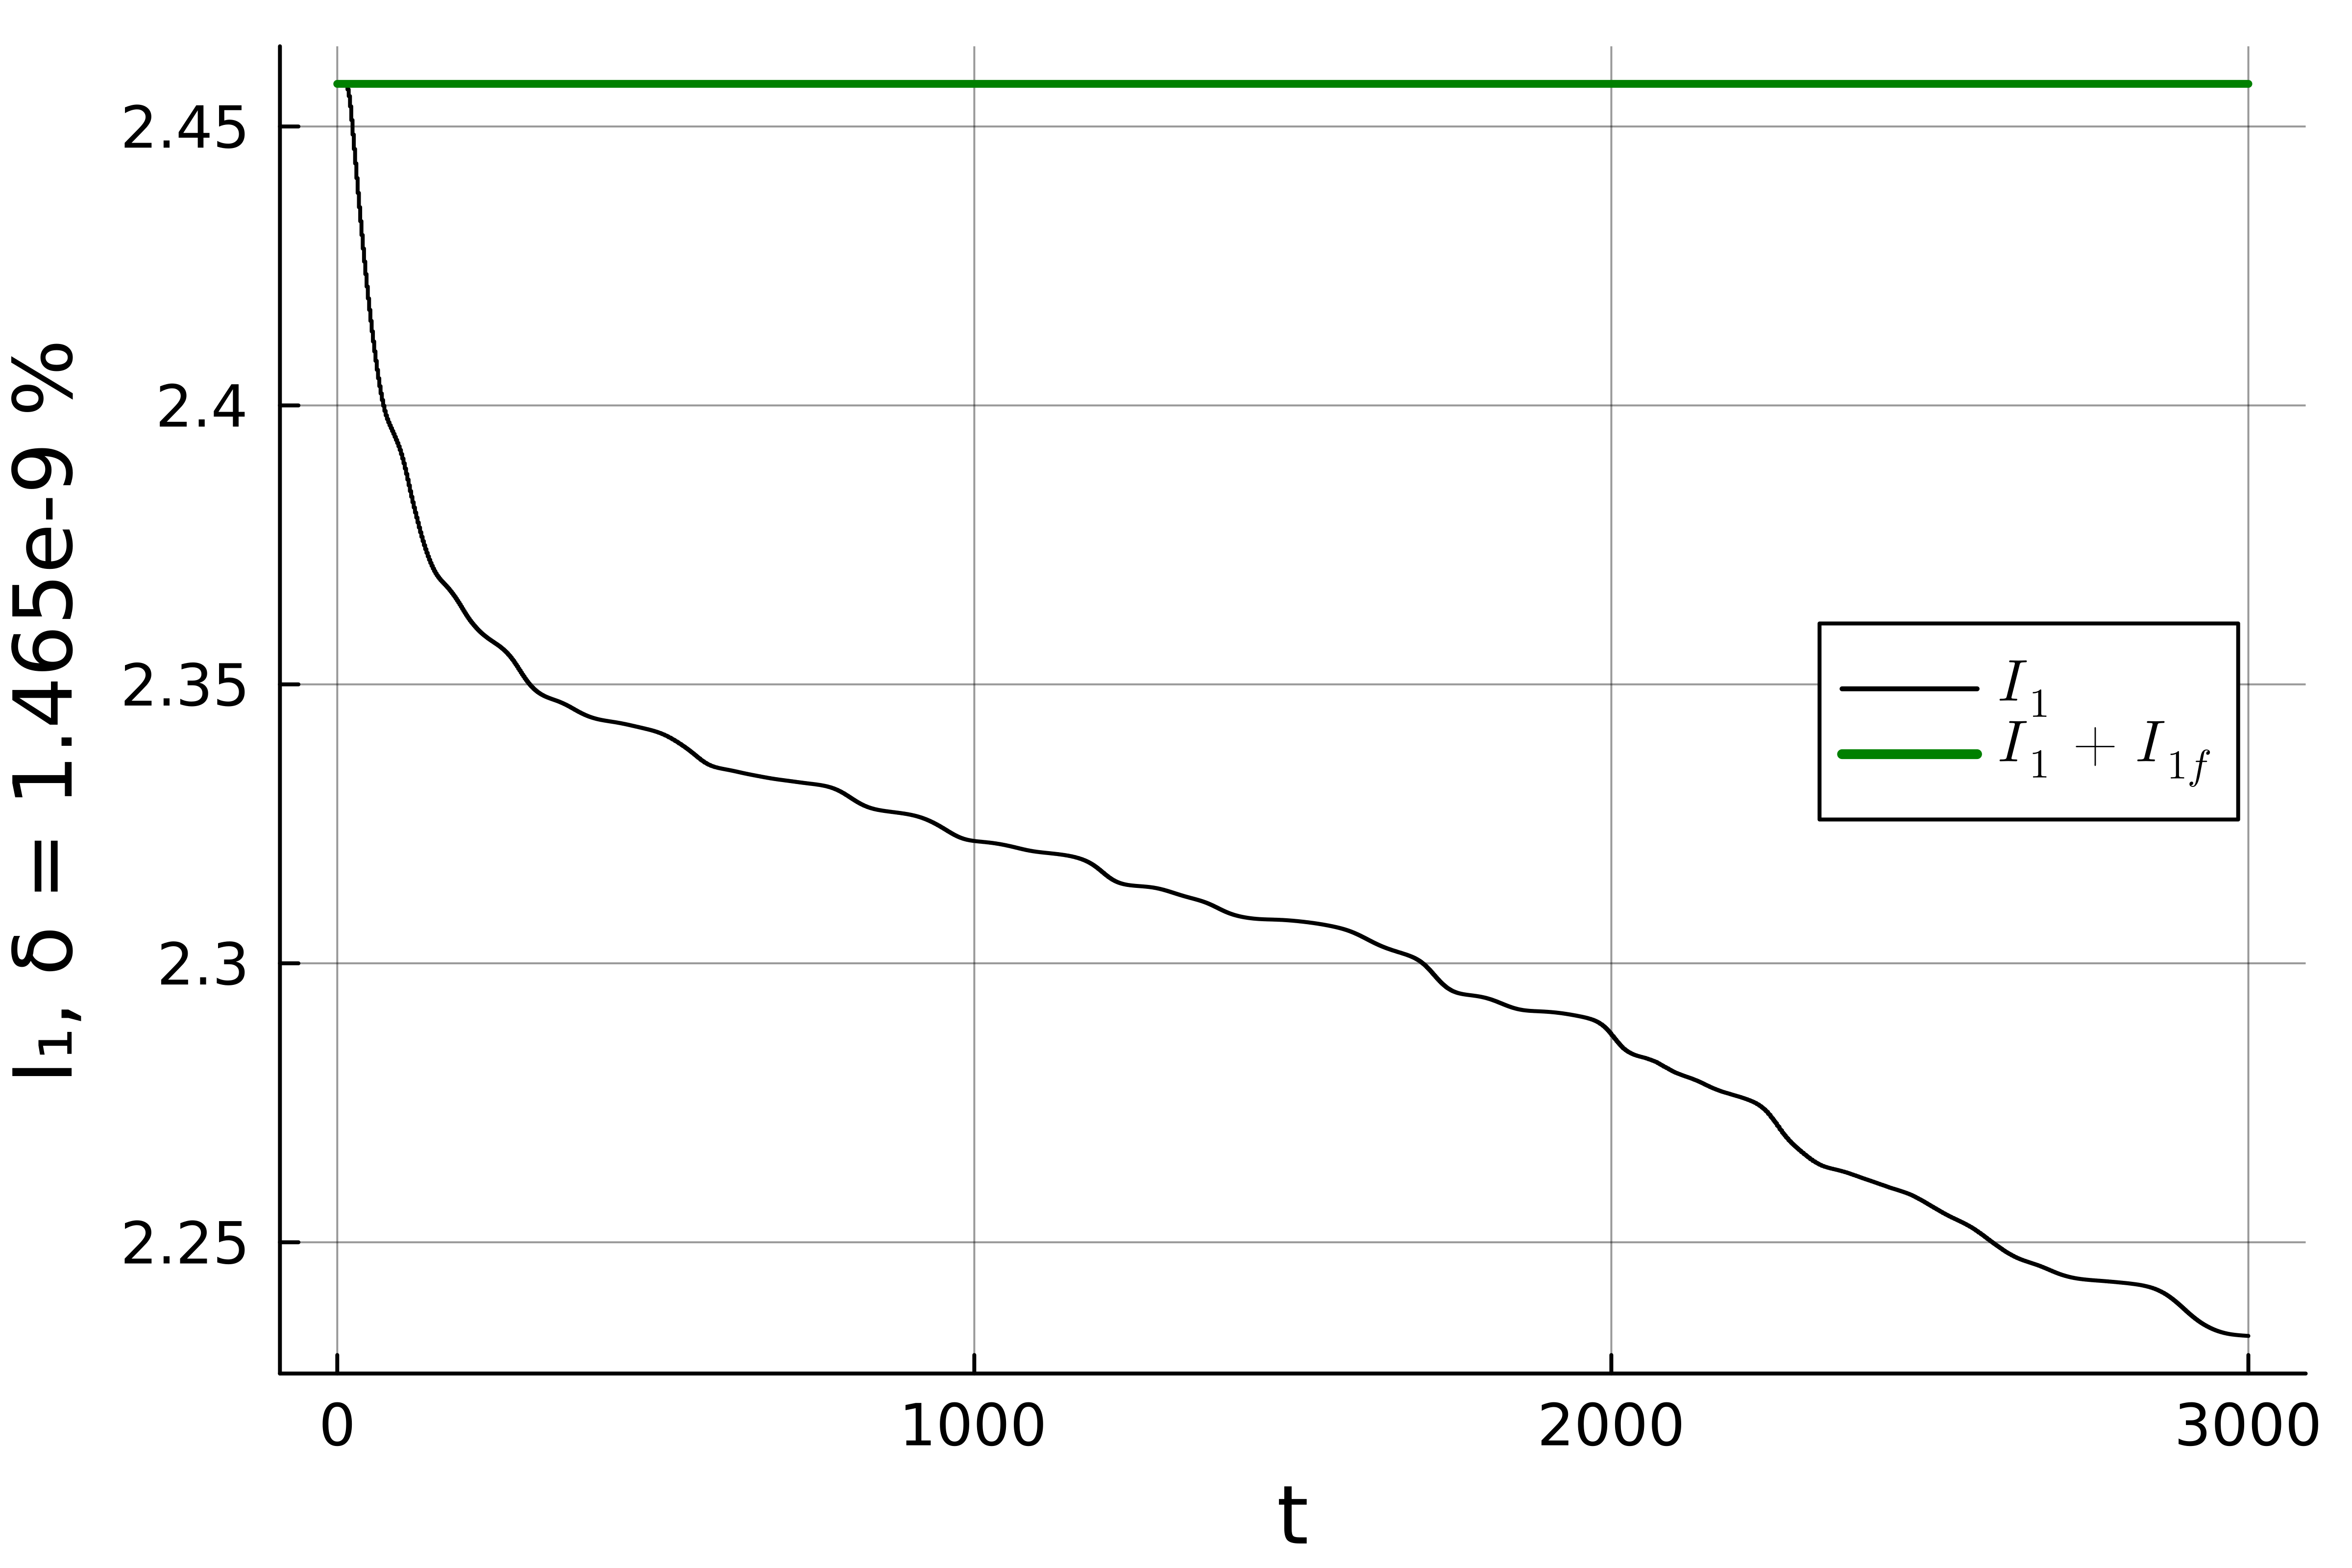
\includegraphics[width=1\linewidth]{fig69.png}
						\subcaption{Зависимость \(I_{1}\) от времени.}
					\end{minipage}
					\hfill
					\begin{minipage}[h]{0.48\linewidth}
						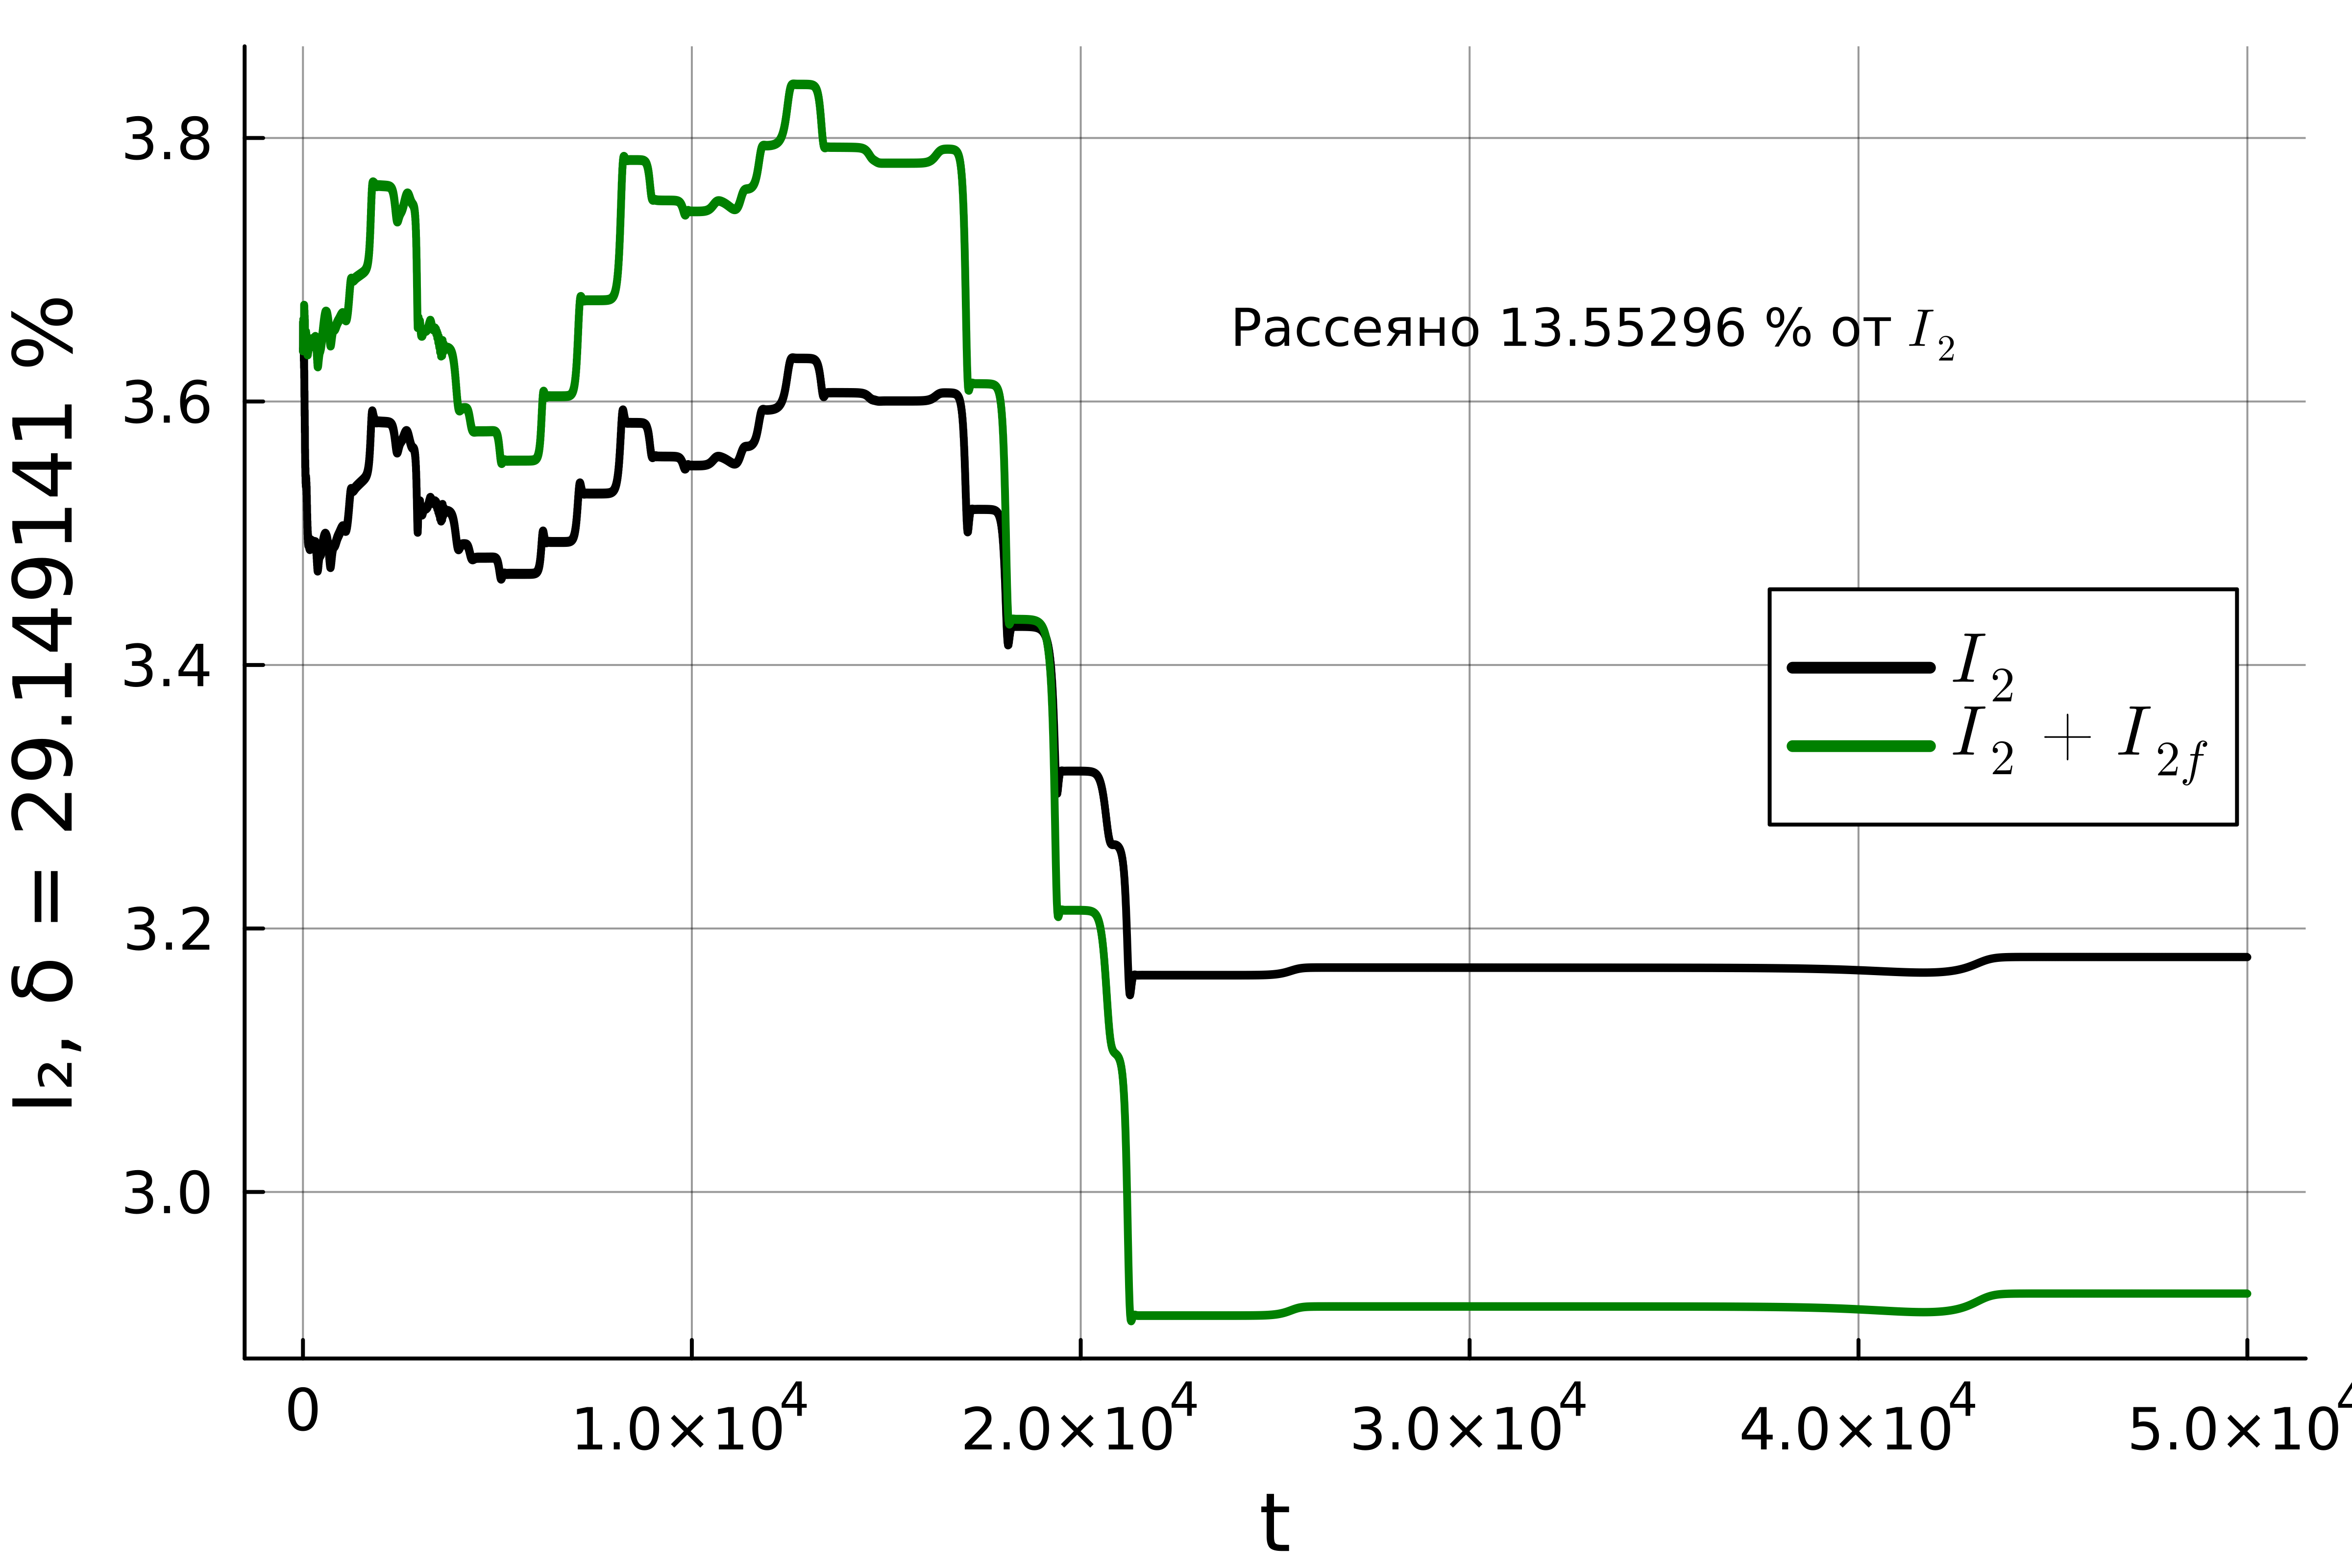
\includegraphics[width=1\linewidth]{fig70.png}
						\subcaption{Зависимость \(I_{2}\) от времени.}
					\end{minipage}
				\end{center}
				\caption{Поведение законов сохранения при
				\(L=160,\, T=50000,\, h=0.2,\, \tau=0.04,\)
				\(\varepsilon_{2}=0.65,\,\varepsilon_{3}=0.08,\, \omega=0.4,\, k=0.15\).}
				\label{fig340-7}
			\end{figure}

			Колебания амплитуды имульса в конце моделирования составили \(0.5\%\), что позволяет сделать вывод, что для того же времени моделирования и параметров импульса, но больших положительных параметрах нелинейностей в модели, чем для расчёта, проиллюстрированного на Рис. \ref{fig340-5_3} процесс перехода к концу моделирования установился хуже. Это согласуется с фактом, что для больших положительных коэффициентов \(\varepsilon_{2}\) и \(\varepsilon_{3}\) процесс устанавливается дольше.

			Несмотря на то, что построить аналитическое решение с точностью порядка \(0.1\%\) по итоговому численному возможно, сделать вывод о сходимости к построенному решению в условиях нарушения законов сохранения не представляется возможным.

			В противоположной ситуации, для отрицательных ненулевых \(\varepsilon_{2}\) и \(\varepsilon_{3}\), в процессе моделирования наблюдается сходимость. Однако решение, построенное в разделе \ref{ch210} не существует для данных параметров. Алгоритм подбора аналитического решения по численному в данном случае не срабатывает, и сравнивать численное решение не с чем. Процесс перехода к моменту \(T=5000\) установился с точностью \(3.7e^{-4}\%\), законы сохранения выполняются, и процесс потери солитоном мощности и импульса постепенно прекращатеся. Зависимости интегралов от времени проиллюстрированы на Рис. \ref{fig340-8}.

			\begin{figure}[H] %% color here
				\begin{center}
					\begin{minipage}[h]{0.48\linewidth}
						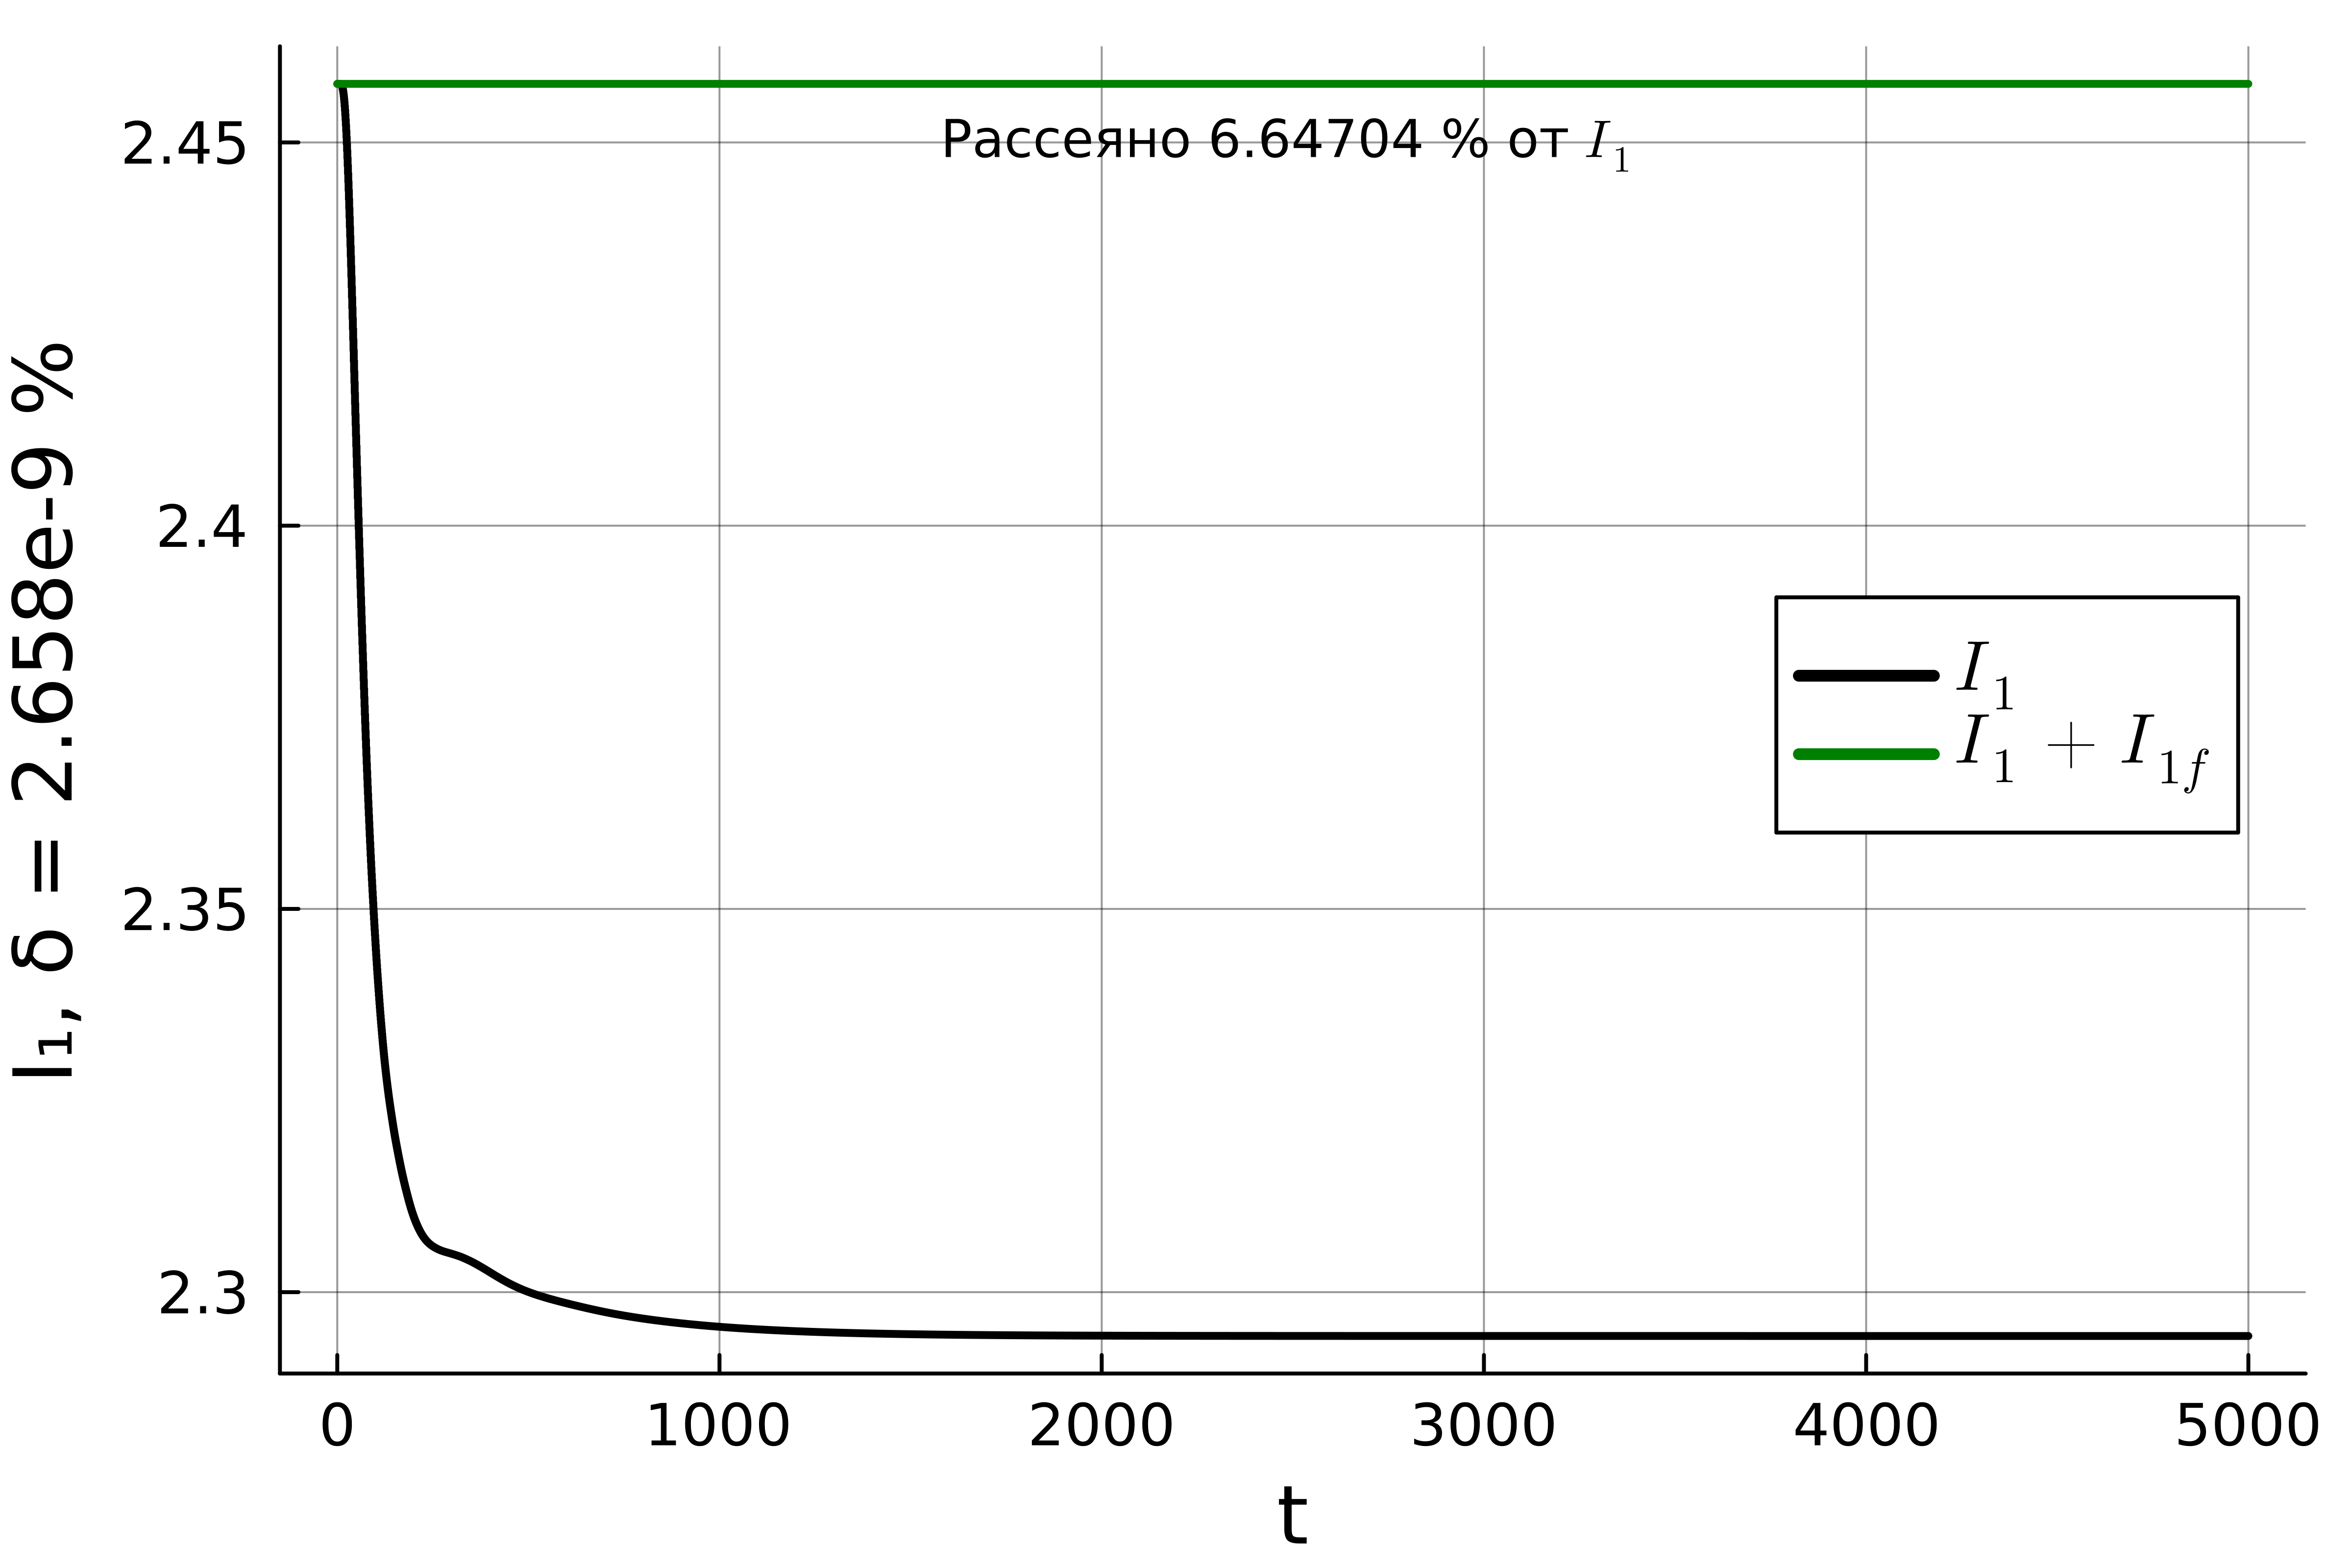
\includegraphics[width=1\linewidth]{fig80.png}
						\subcaption{Зависимость \(I_{1}\) от времени.}
					\end{minipage}
					\hfill
					\begin{minipage}[h]{0.48\linewidth}
						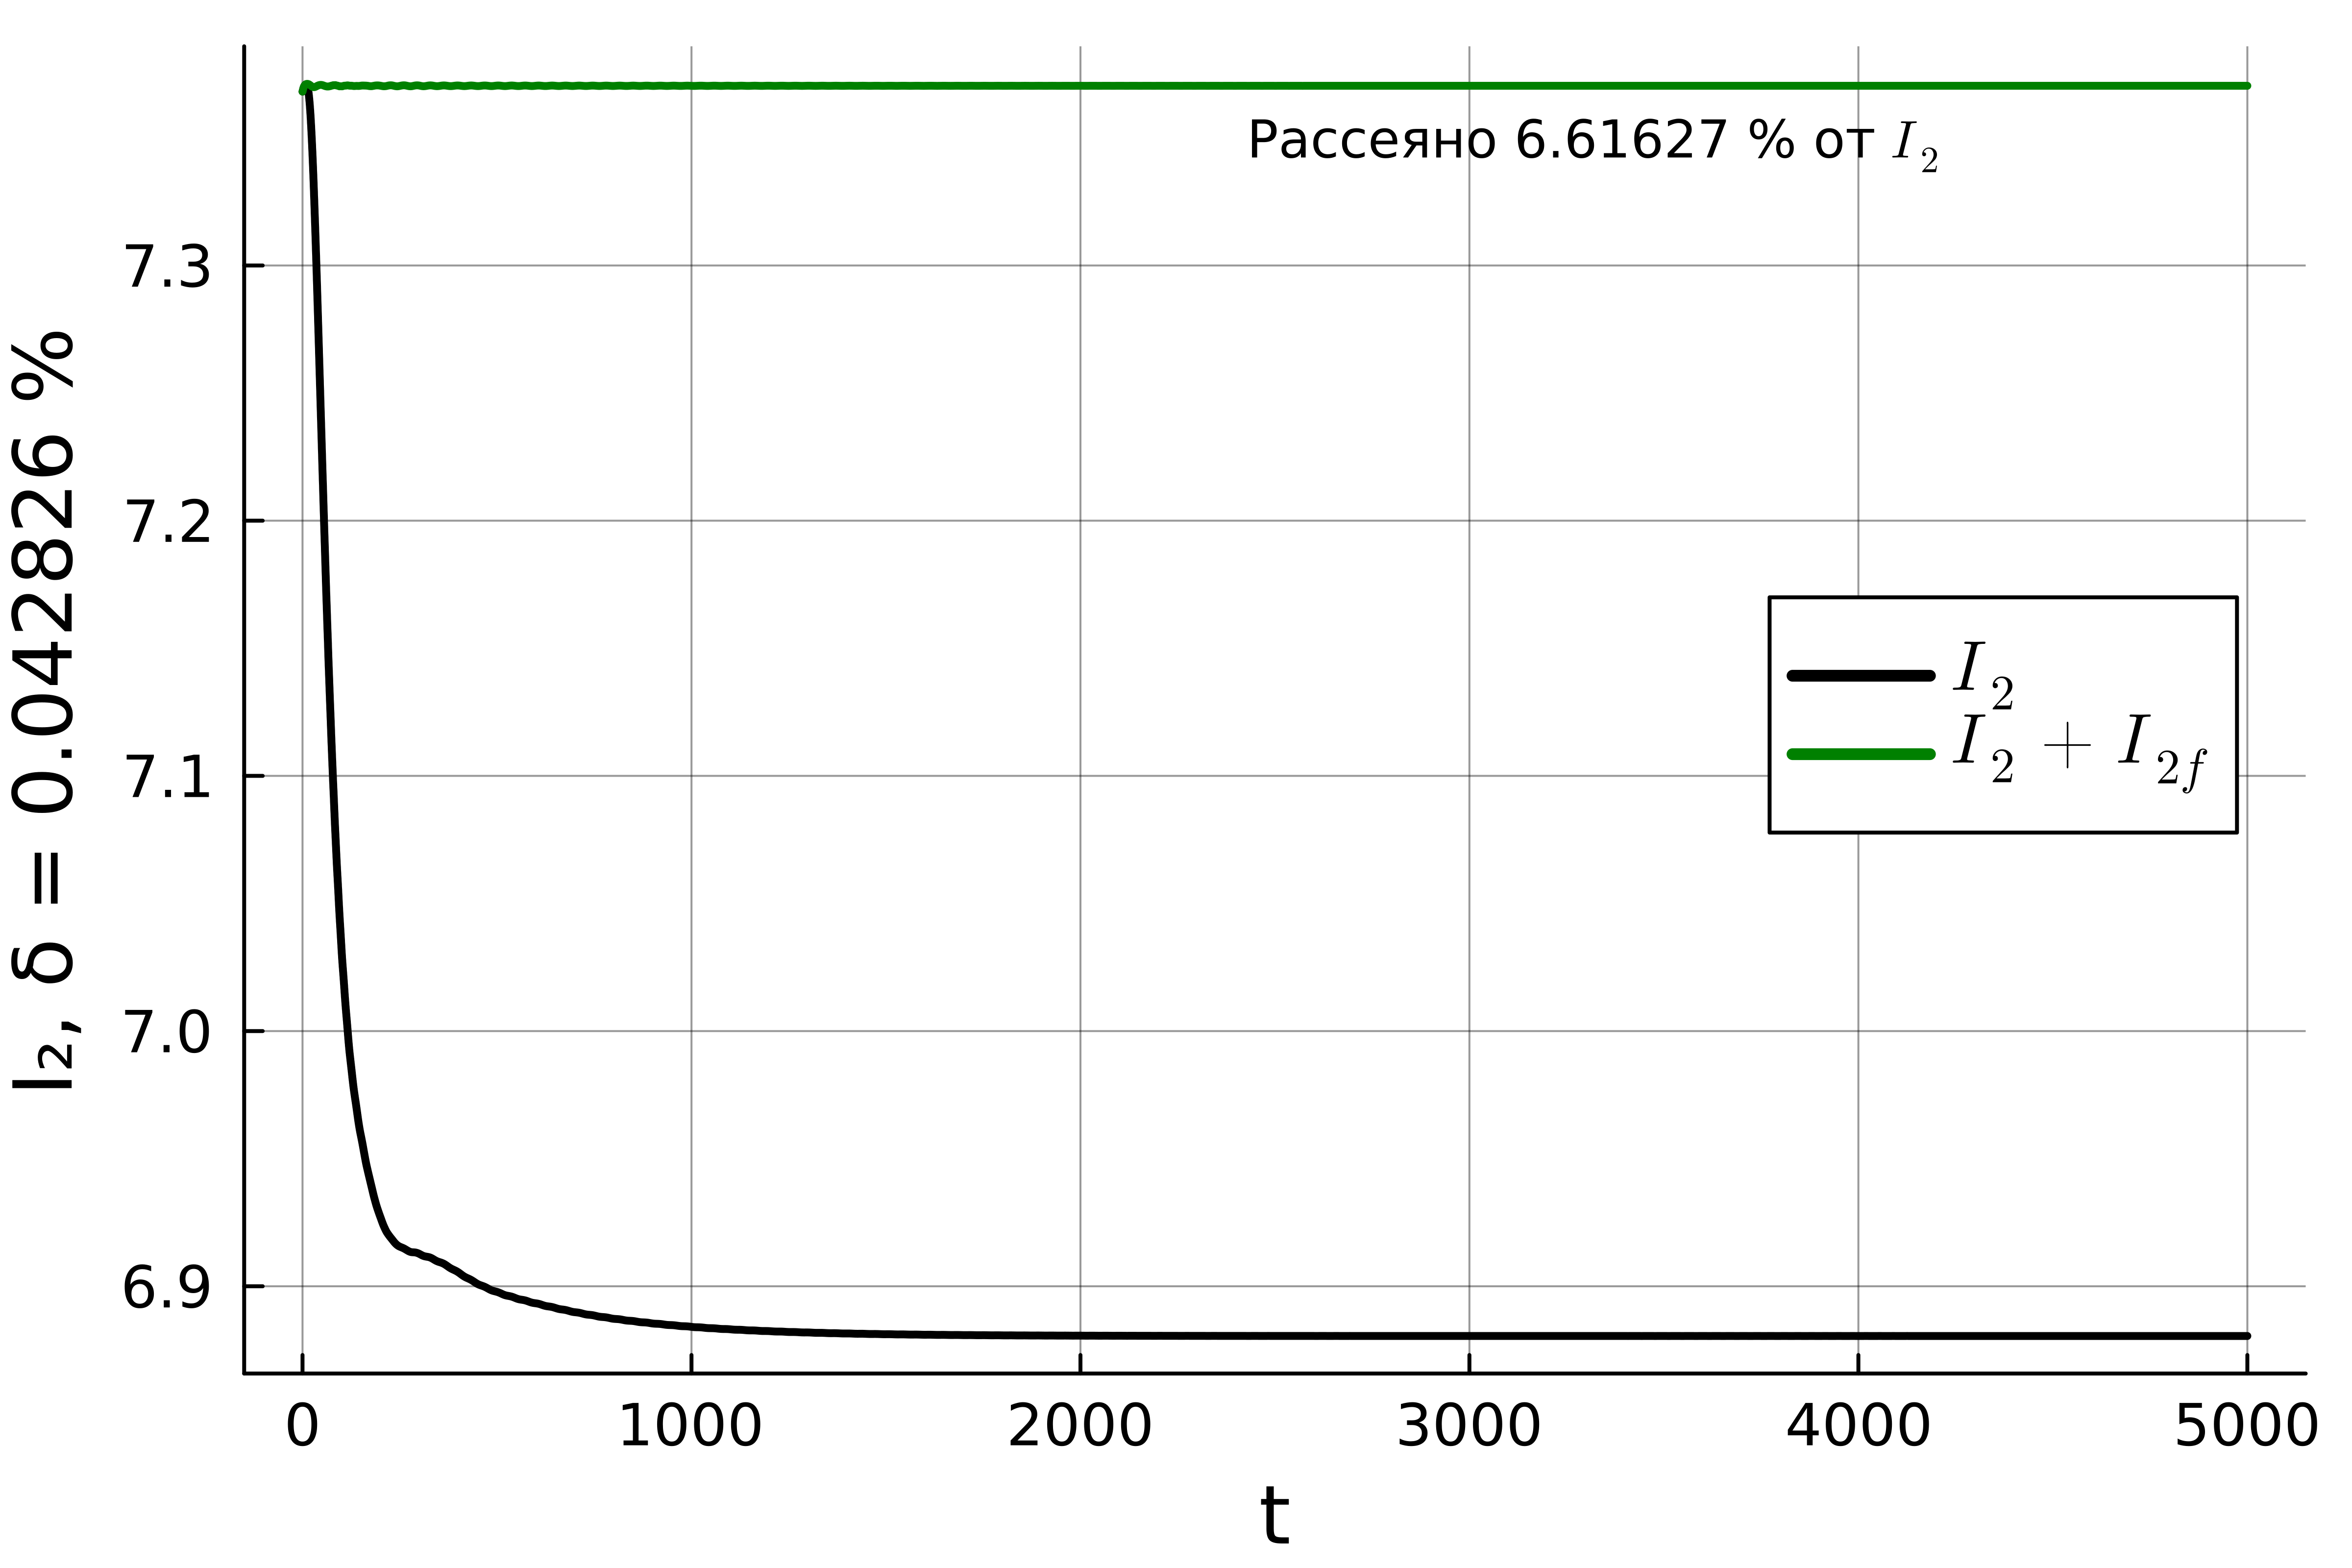
\includegraphics[width=1\linewidth]{fig81.png}
						\subcaption{Зависимость \(I_{2}\) от времени.}
					\end{minipage}
				\end{center}
				\caption{Поведение законов сохранения при
				\(L=160,\, T=5000,\, h=0.1,\, \tau=0.02,\)
				\(\varepsilon_{2}=-0.65,\,\varepsilon_{3}=-0.08,\, \omega=0.4,\, k=0.15\).}
				\label{fig340-8}
			\end{figure}

			Несмотря на отсутствие аналитического решения, мы утверждаем, что сходимость численного решения достигнута. Законы сохранения выполняются, потери солитоном интегралов прекращаются - за вторую половину моделирования рассеяно в \(23e^{3}\) раз меньше \(I_{1}\), чем в первую, и аналогично, в \(27e^{3}\) раз меньше \(I_{2}\). Амплитуда численного решения устанавливается. Её поведение проиллюстрировано на Рис. \ref{fig340-9}.

			\begin{figure}[H]
				\begin{center}
					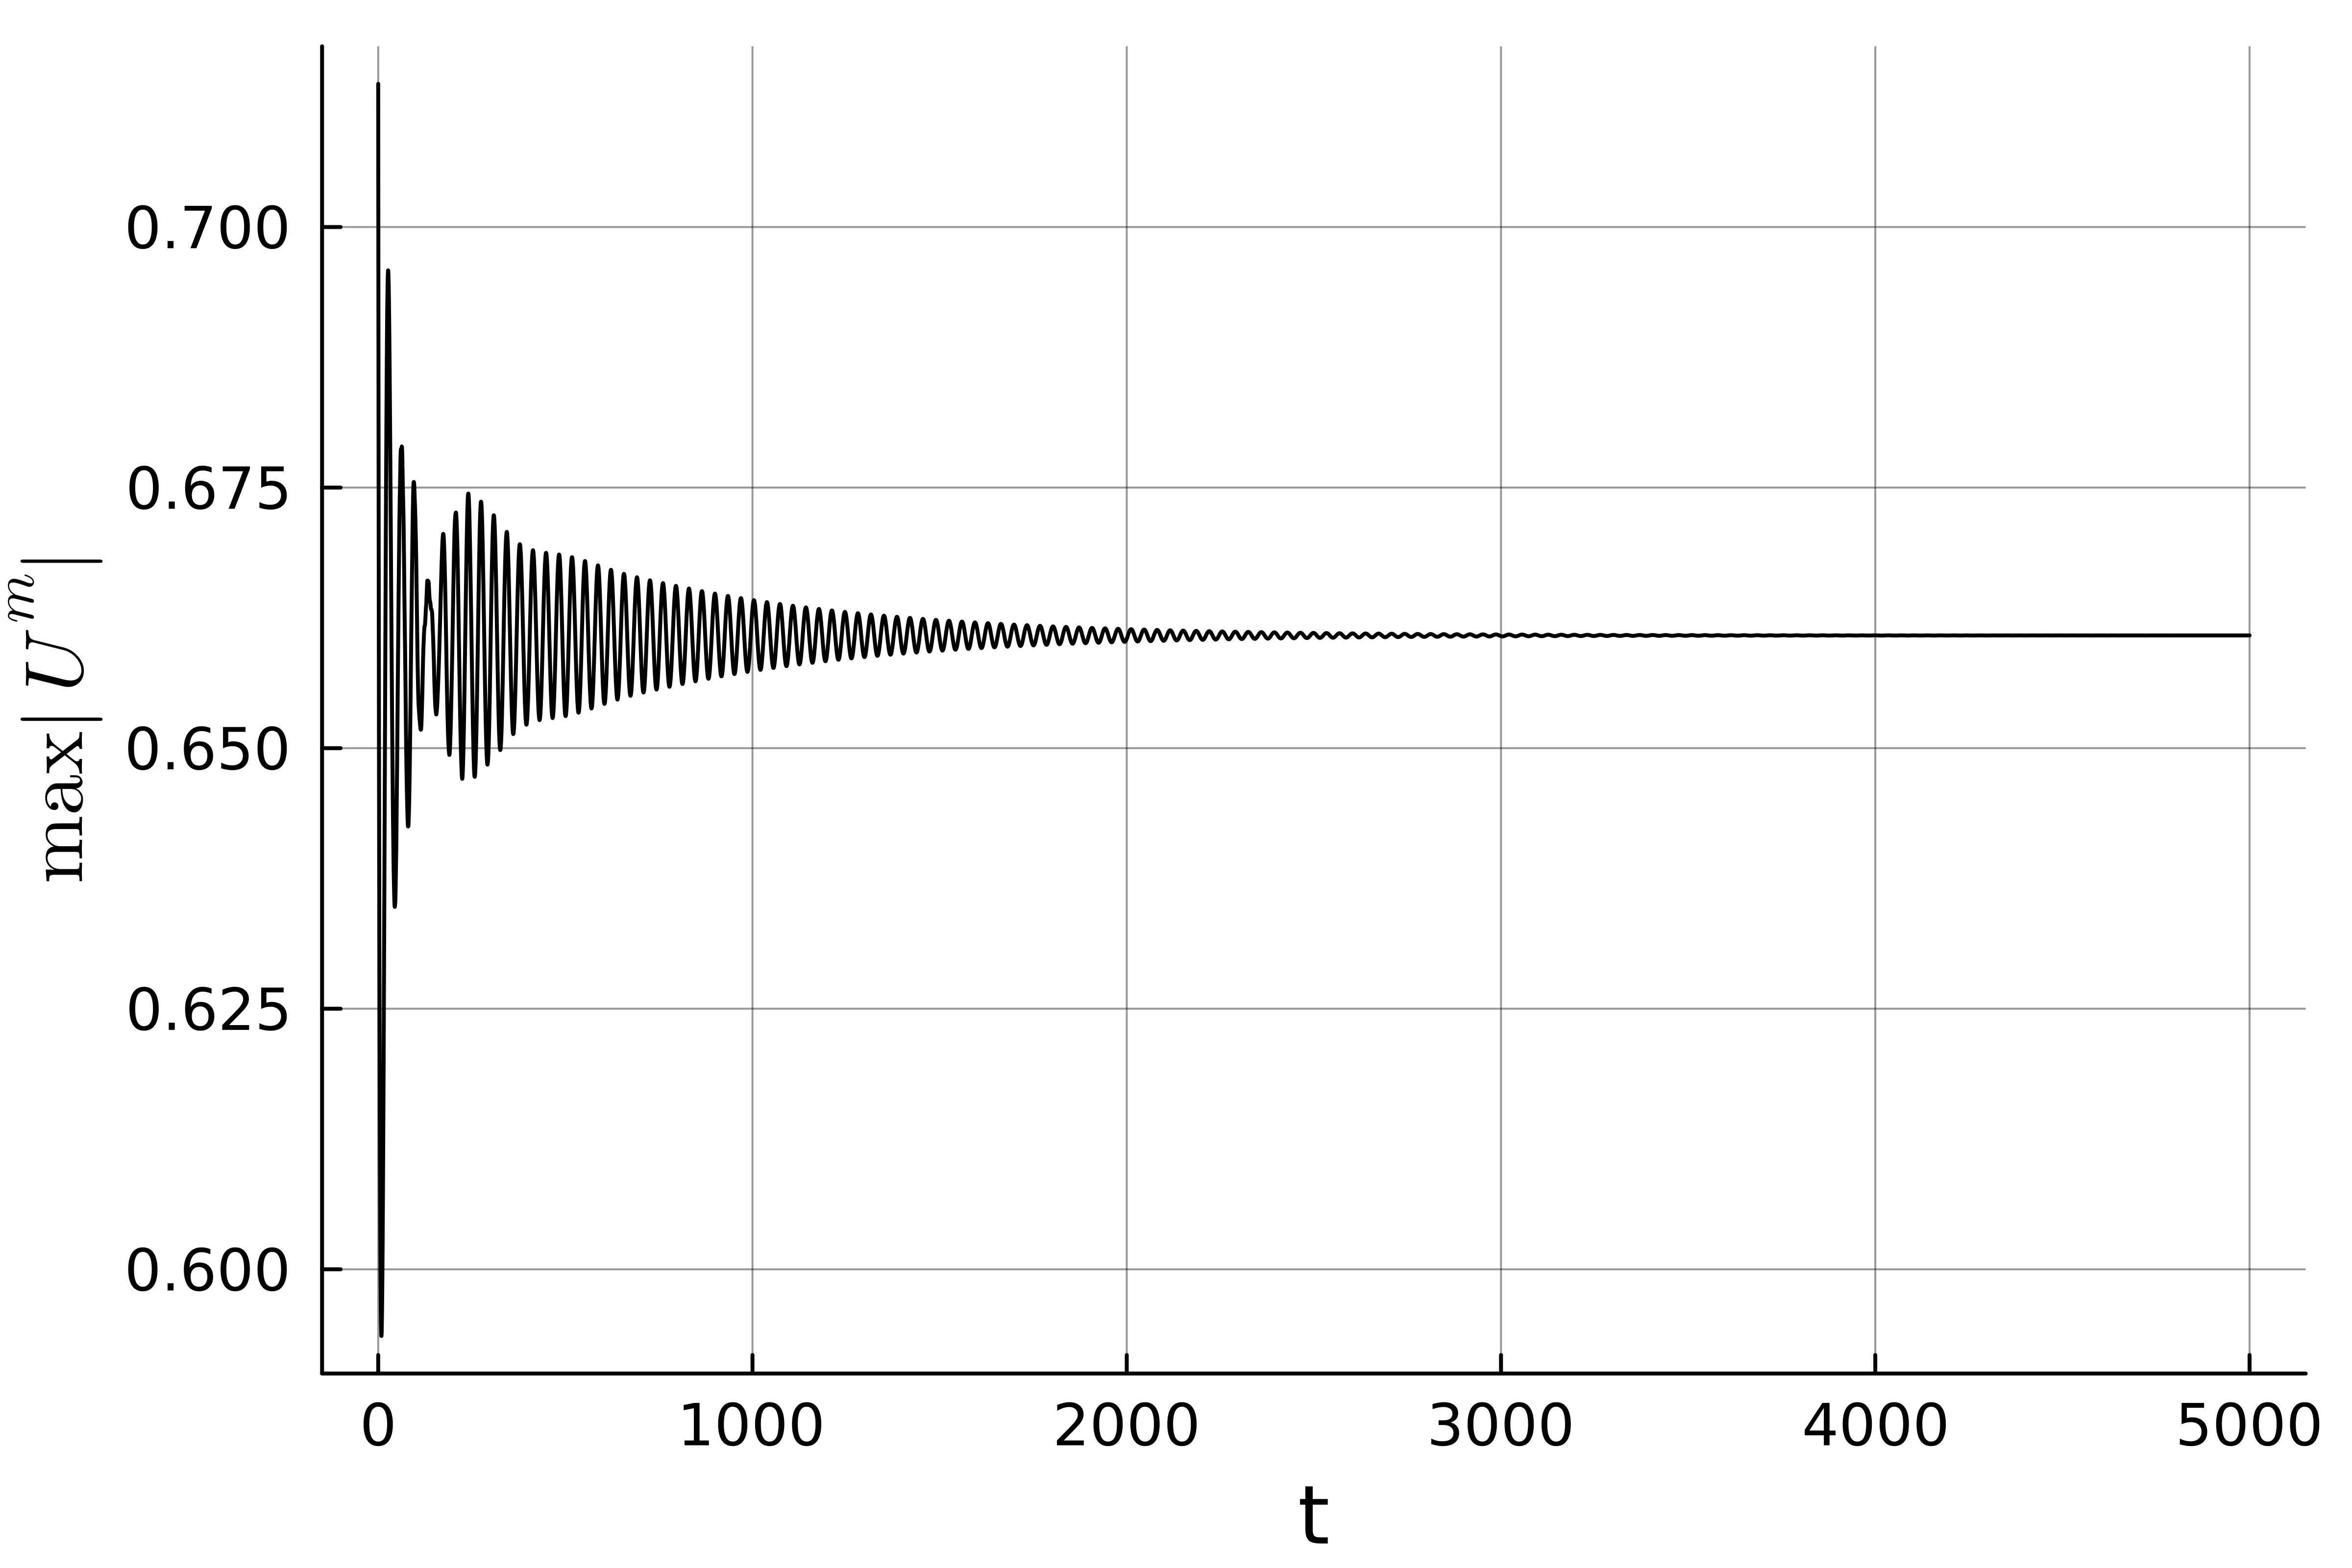
\includegraphics[width=0.5\linewidth]{fig82.png}
				\end{center}
				\caption{Зависимость амплитуды численного решения от времени при
				\(L=160,\, T=5000,\, h=0.1,\, \tau=0.01,\)
				\(\varepsilon_{2}=-0.65,\,\varepsilon_{3}=-0.08,\, \omega=0.4,\, k=0.15\).}
				\label{fig340-9}
			\end{figure}

			Определив влияние одновременно отрицательных или одновременно положительных \(\varepsilon_{2}\) и \(\varepsilon_{3}\), возможно предположить, что комбинации в математической модели параметров разных знаков будет иметь усреднённые свойства, характерные для параметров каждого знака. Положительные значения стремятся нарушить сеточную сходимость и законы сохранения, привести к большим временам установления. Отрицательные значения, возможно, будут невелировать этот эффект.

			Проиллюстрируем некоторые варианты поведения амплитуды импульса в зависимости от параметров нелинейностей на Рис. \ref{fig481} и Рис. \ref{fig482}. Здесь \(\delta\) — процент, в пределах которого изменяется амплитуда импульса в конце временного промежутка моделирования. Величина \(\delta\) приведена только для условно устанавливающихся переходных процессах.
			\begin{figure}[H] %% color here
				\begin{minipage}[h]{1\linewidth}
					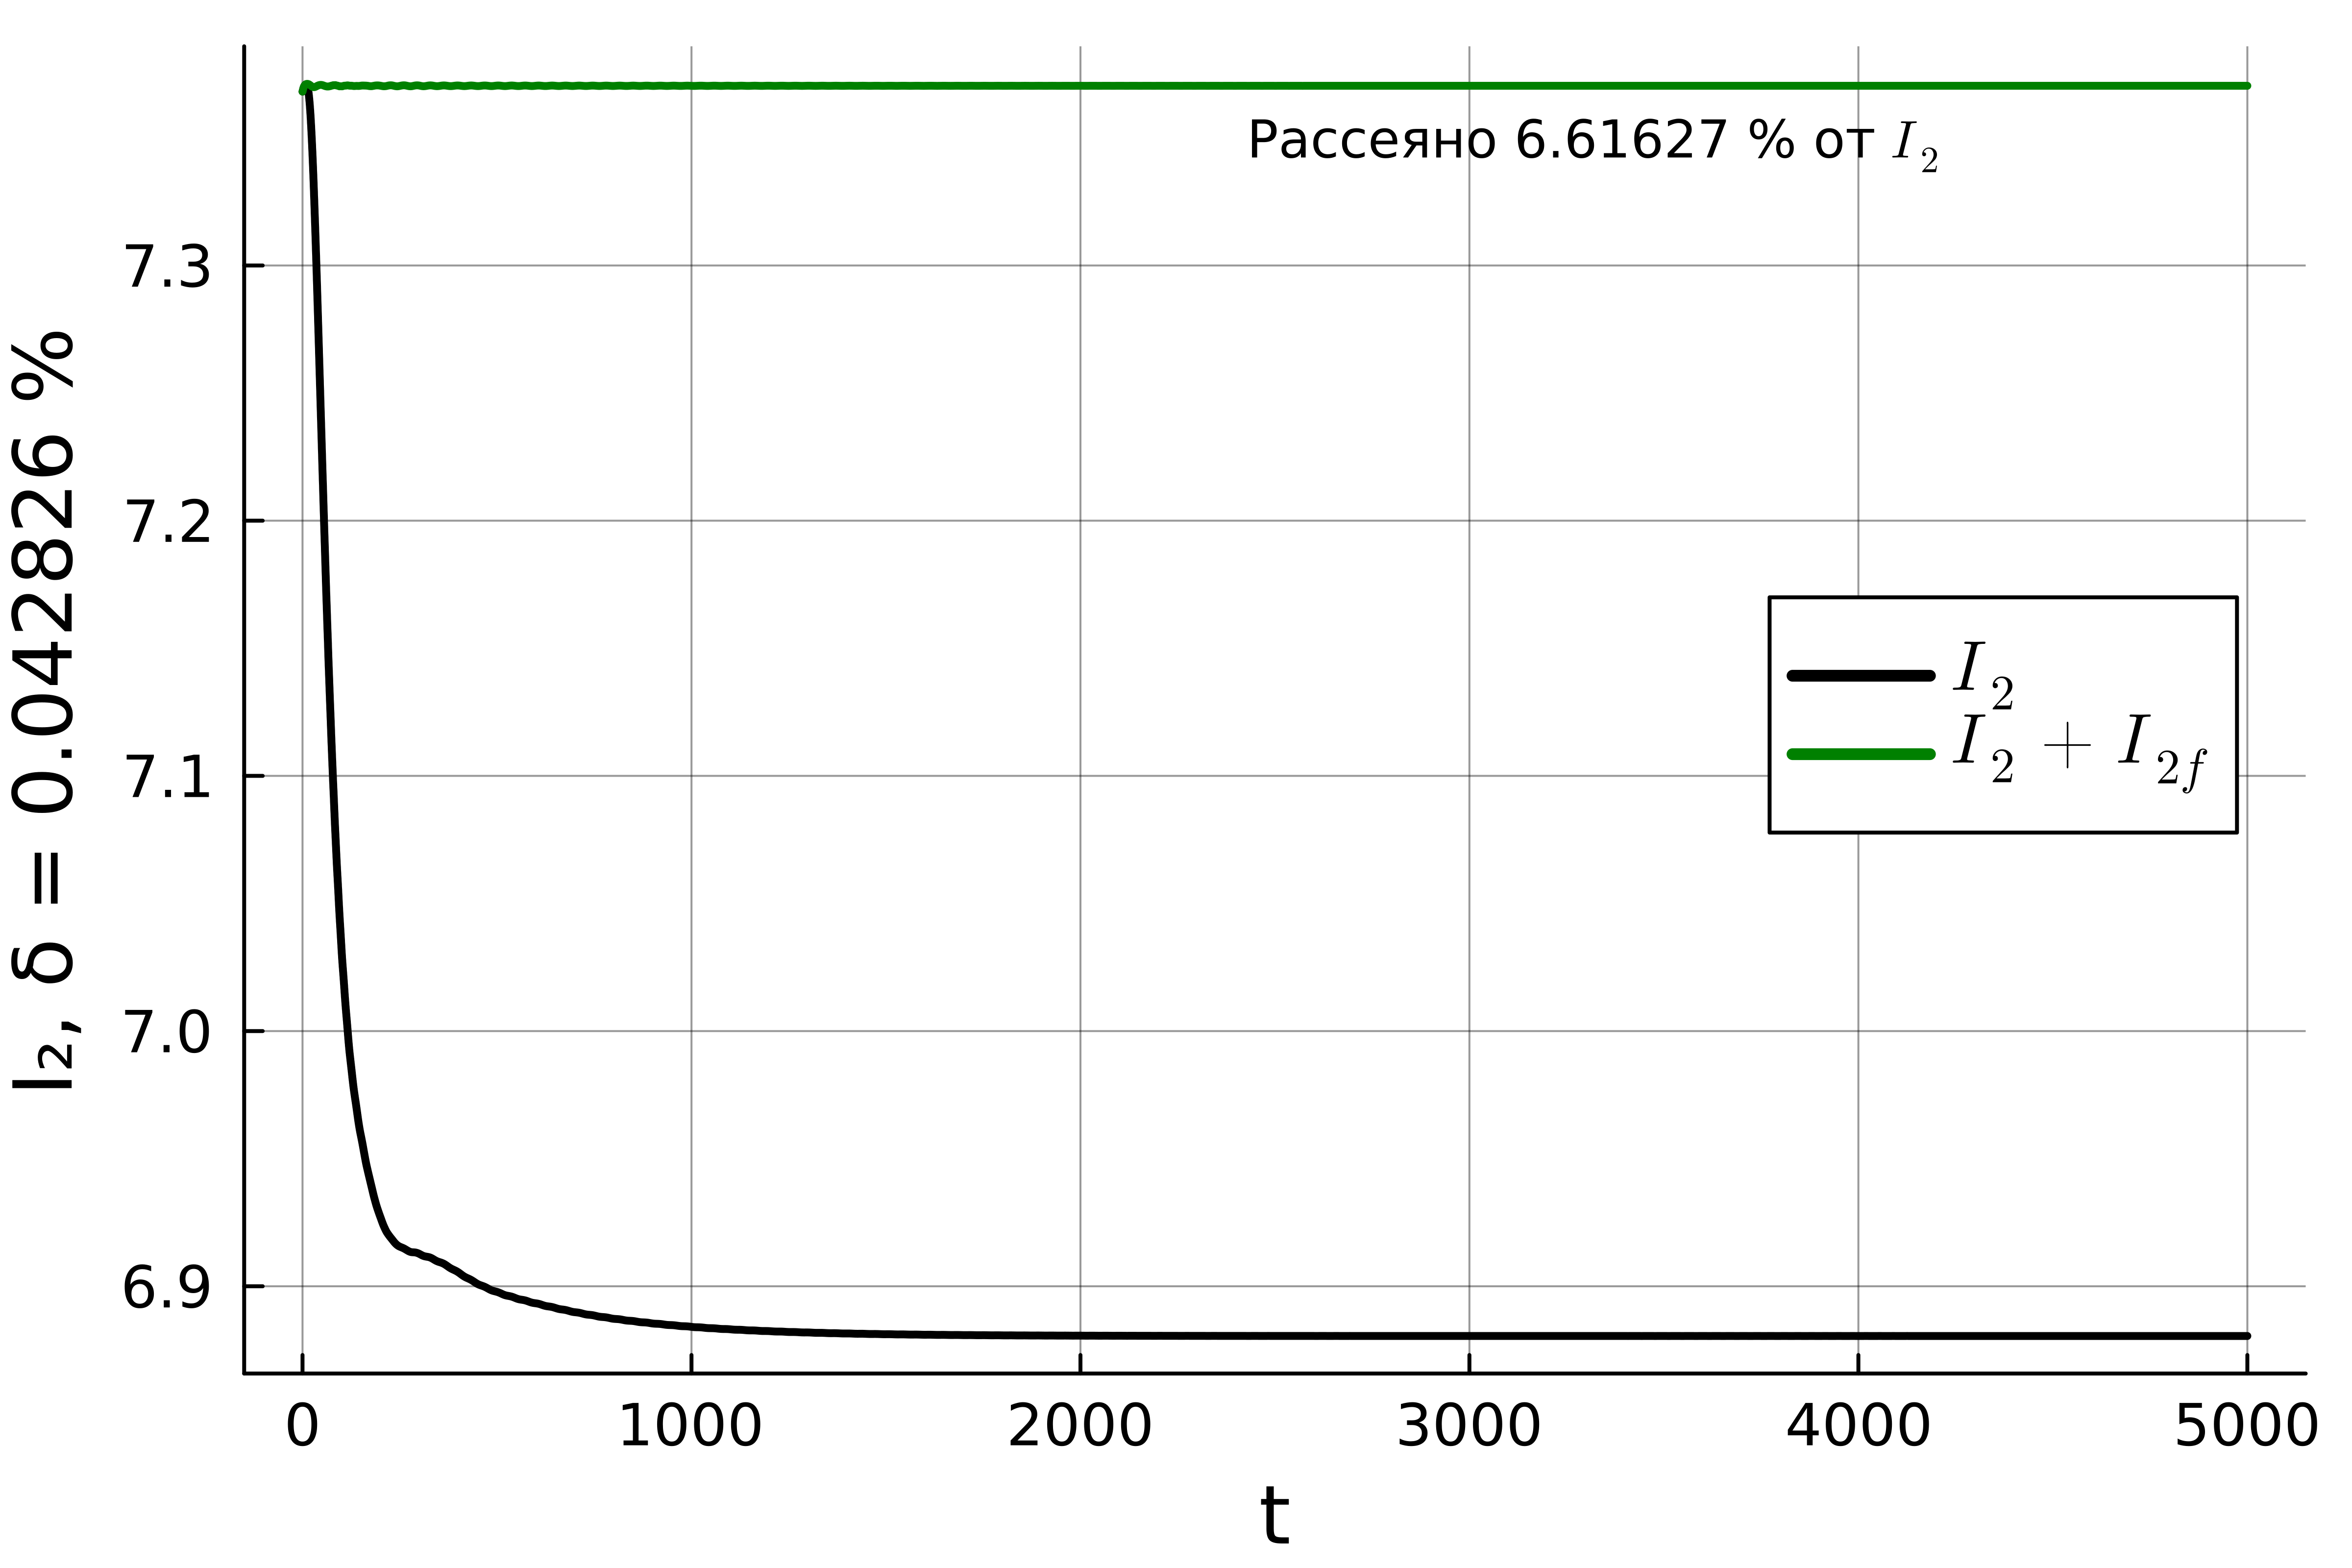
\includegraphics[width=1\linewidth]{fig35.png}
					\subcaption{\(\varepsilon_{2}=-0.5,\,\varepsilon_{3}=0.1\)}
					\label{fig48_1}
					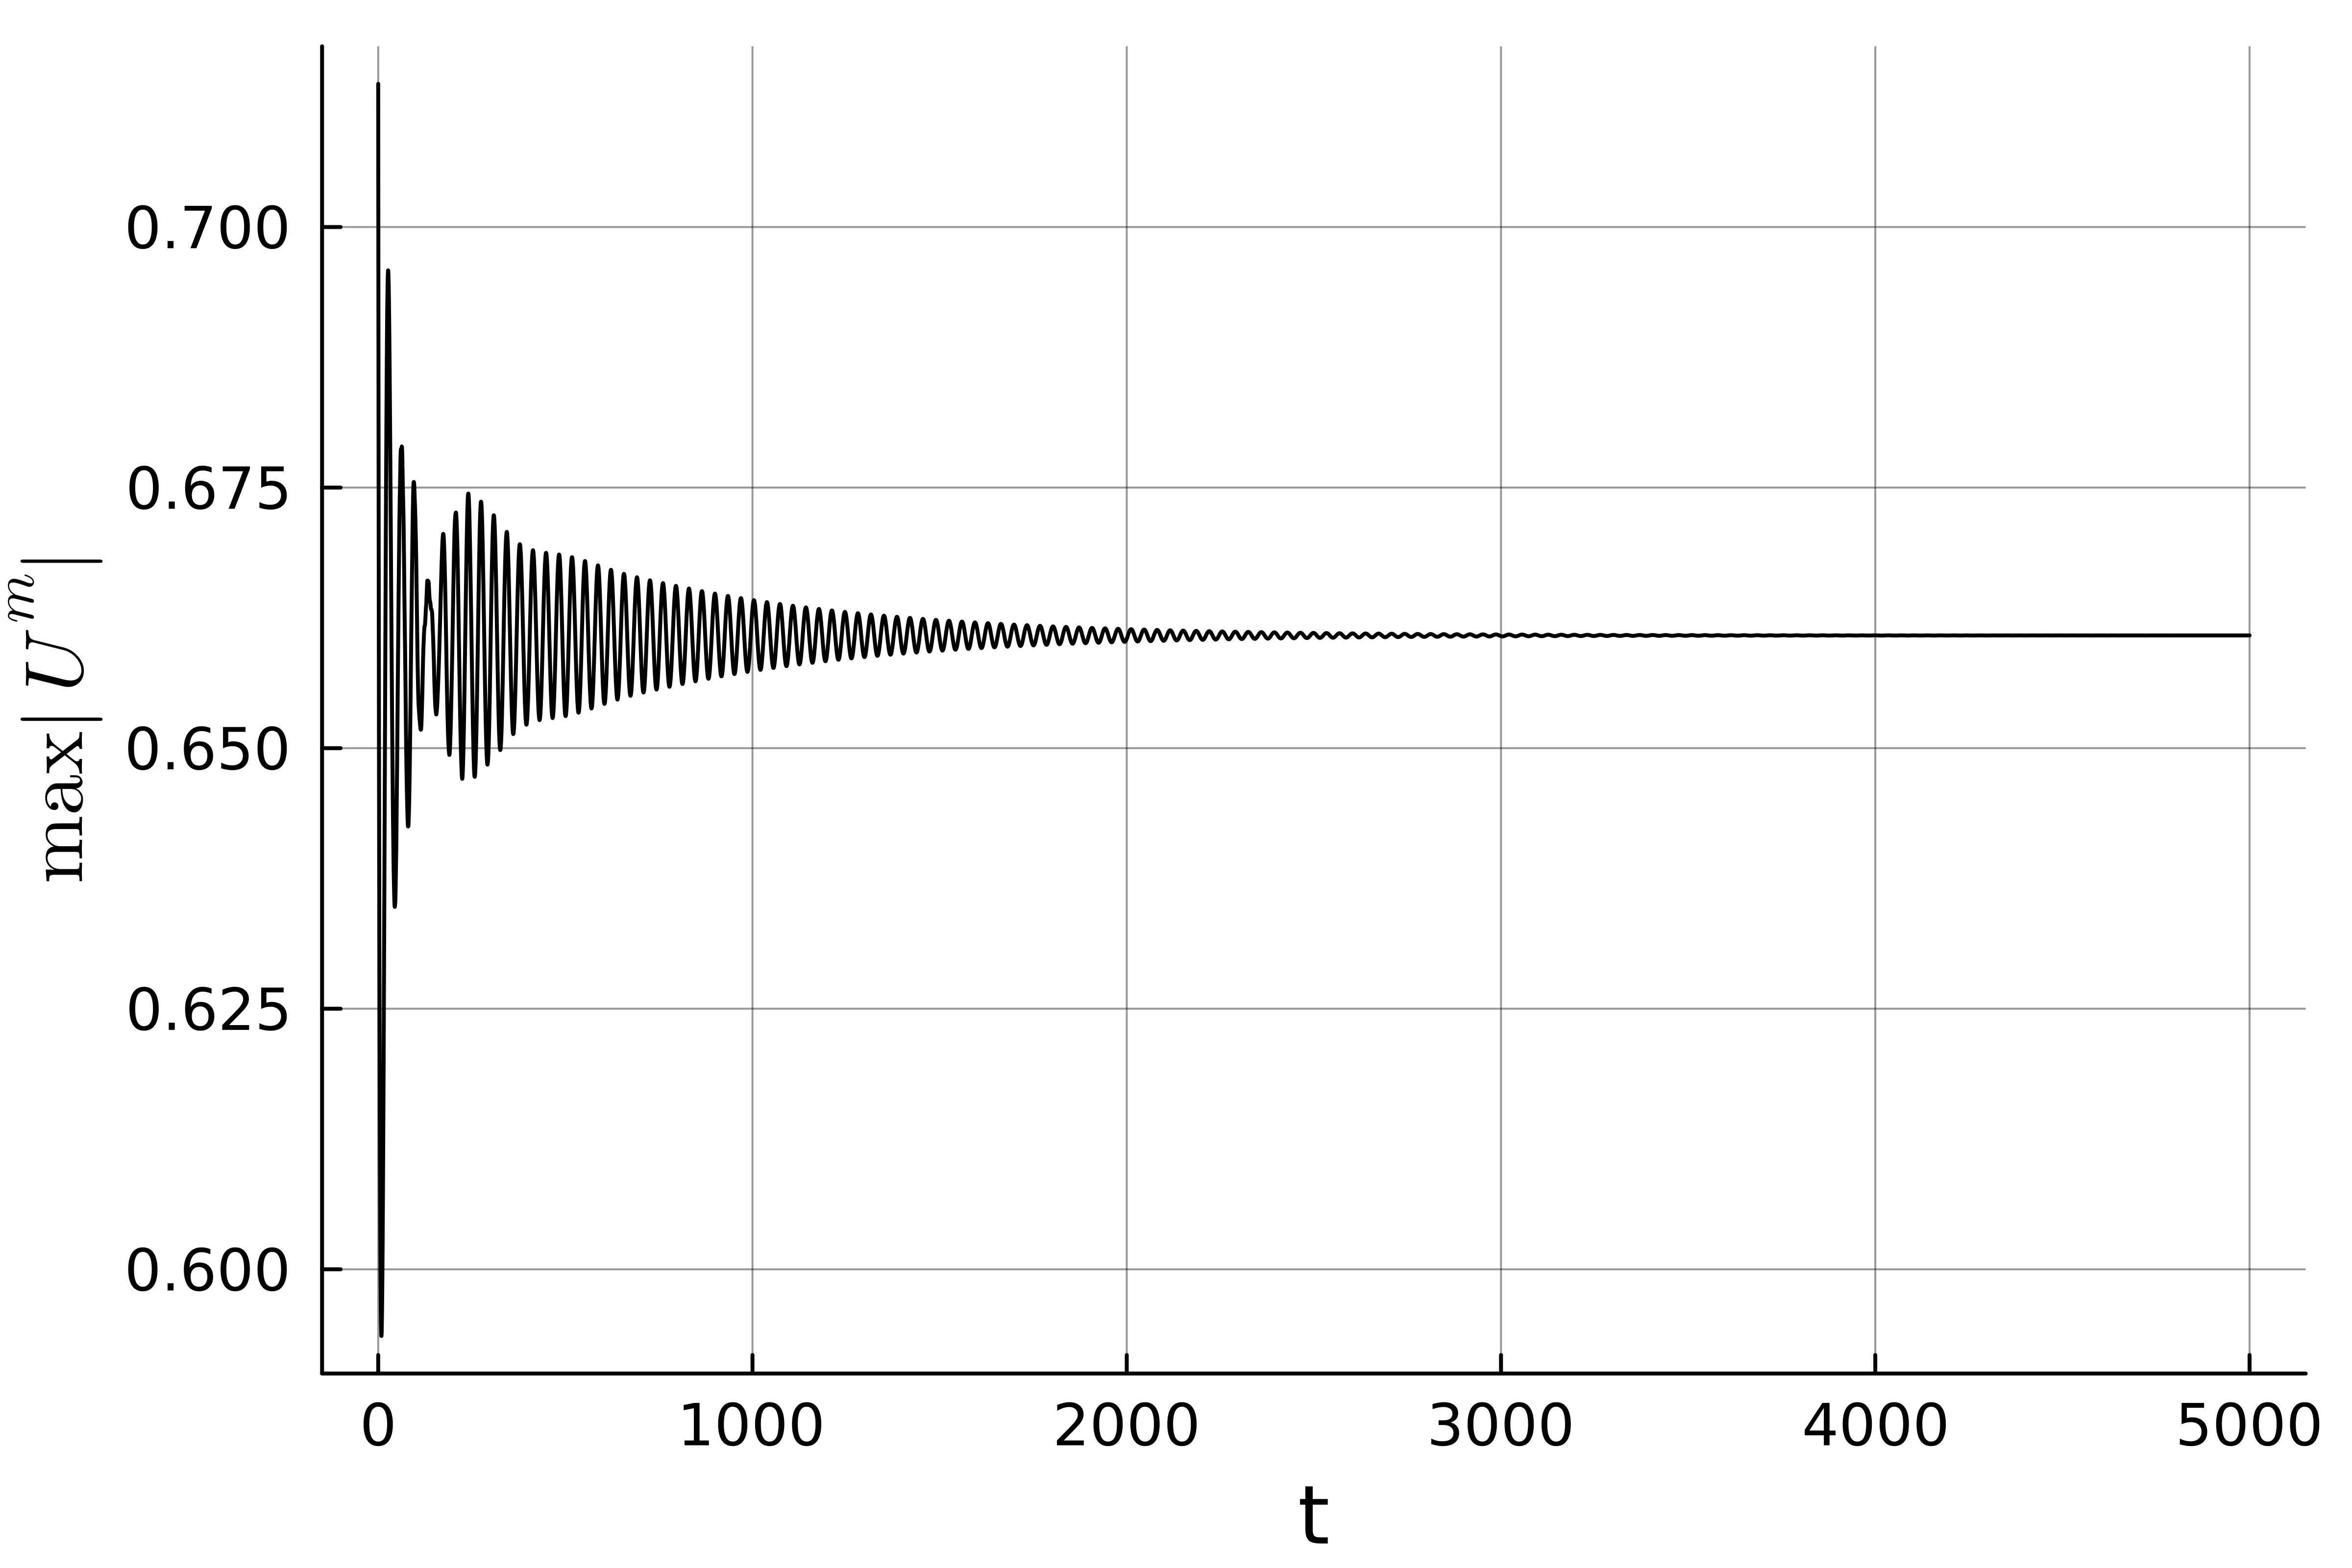
\includegraphics[width=1\linewidth]{fig36.png}
					\subcaption{\(\varepsilon_{2}=-0.5,\,\varepsilon_{3}=0.3\)}
					\label{fig48_2}
					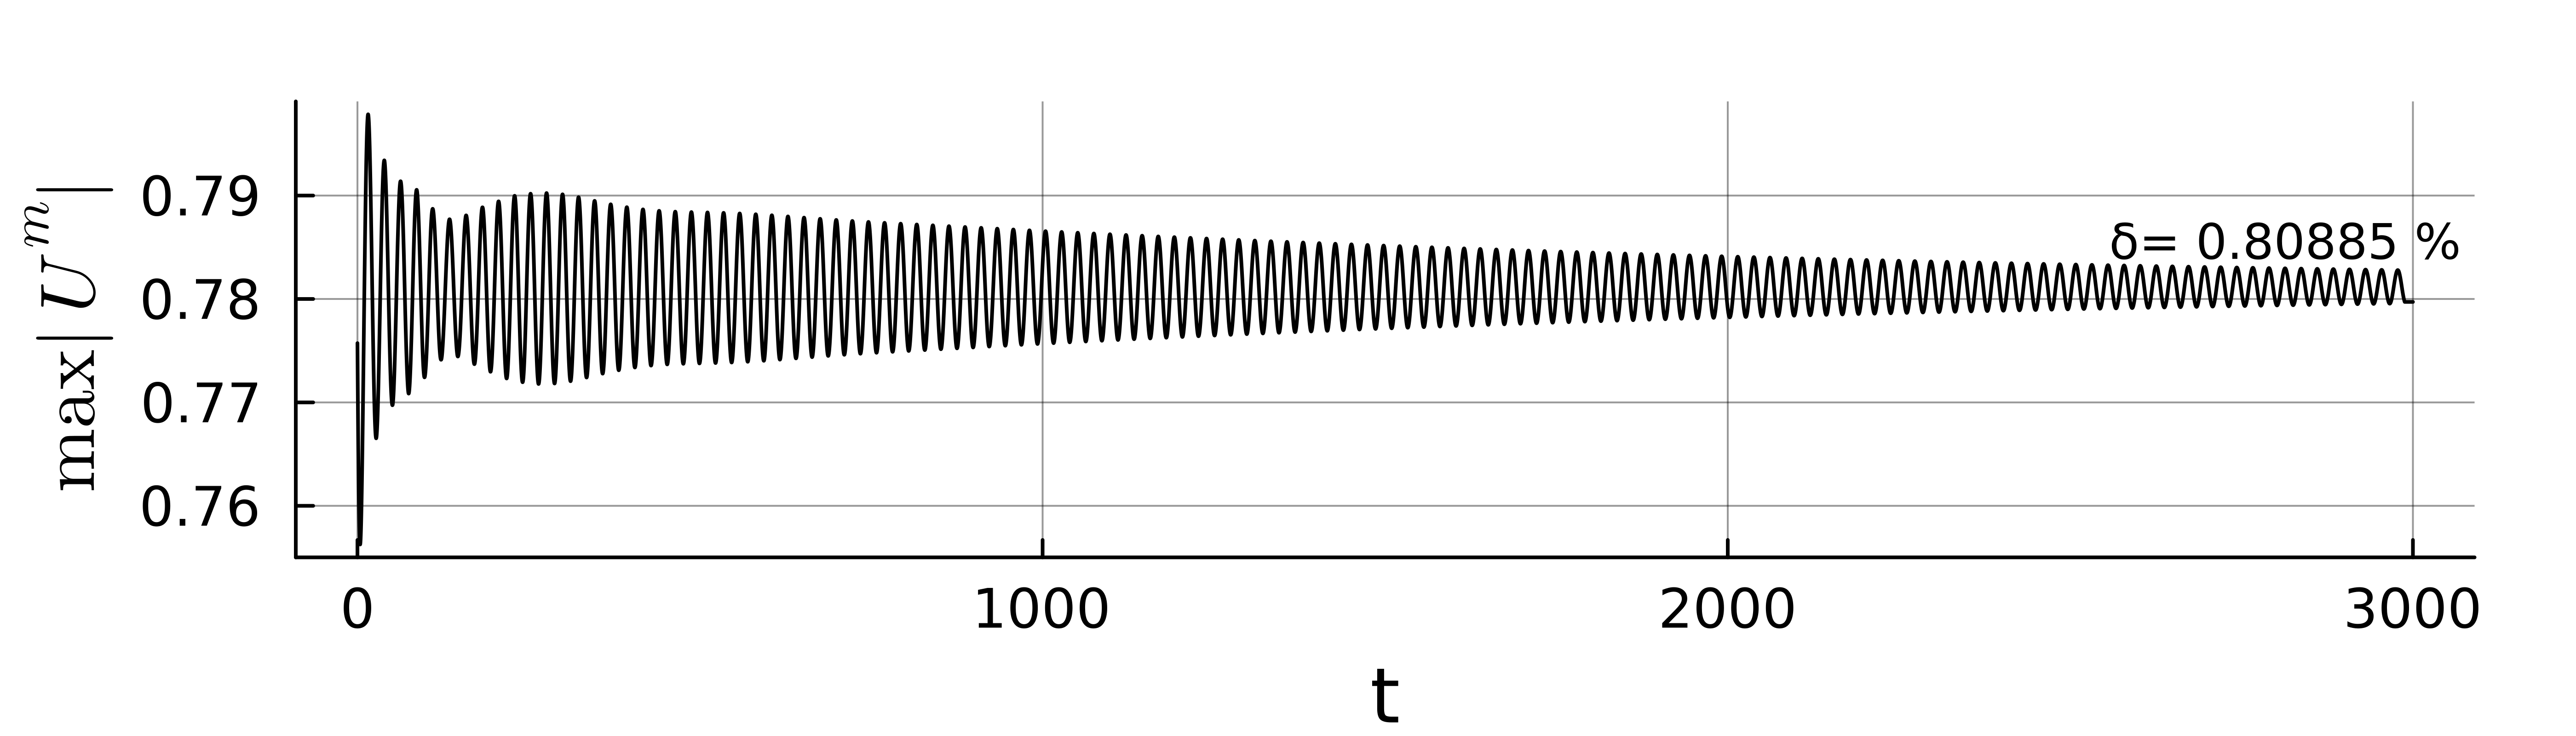
\includegraphics[width=1\linewidth]{fig84.png}
					\subcaption{\(\varepsilon_{2}=-0.5,\,\varepsilon_{3}=0.4\)}
					\label{fig48_3}
				\end{minipage}
				\caption{Зависимость амплитуды импульса (\ref{eq55}) при распространении .
				\(L=160,\, T=3000,\, h=0.2,\, \tau=0.04,\, \omega=0.4,\, k=0.15\).}
				\label{fig481}
			\end{figure}
			\begin{figure}[H] %% color here
				\begin{minipage}[h]{1\linewidth}
					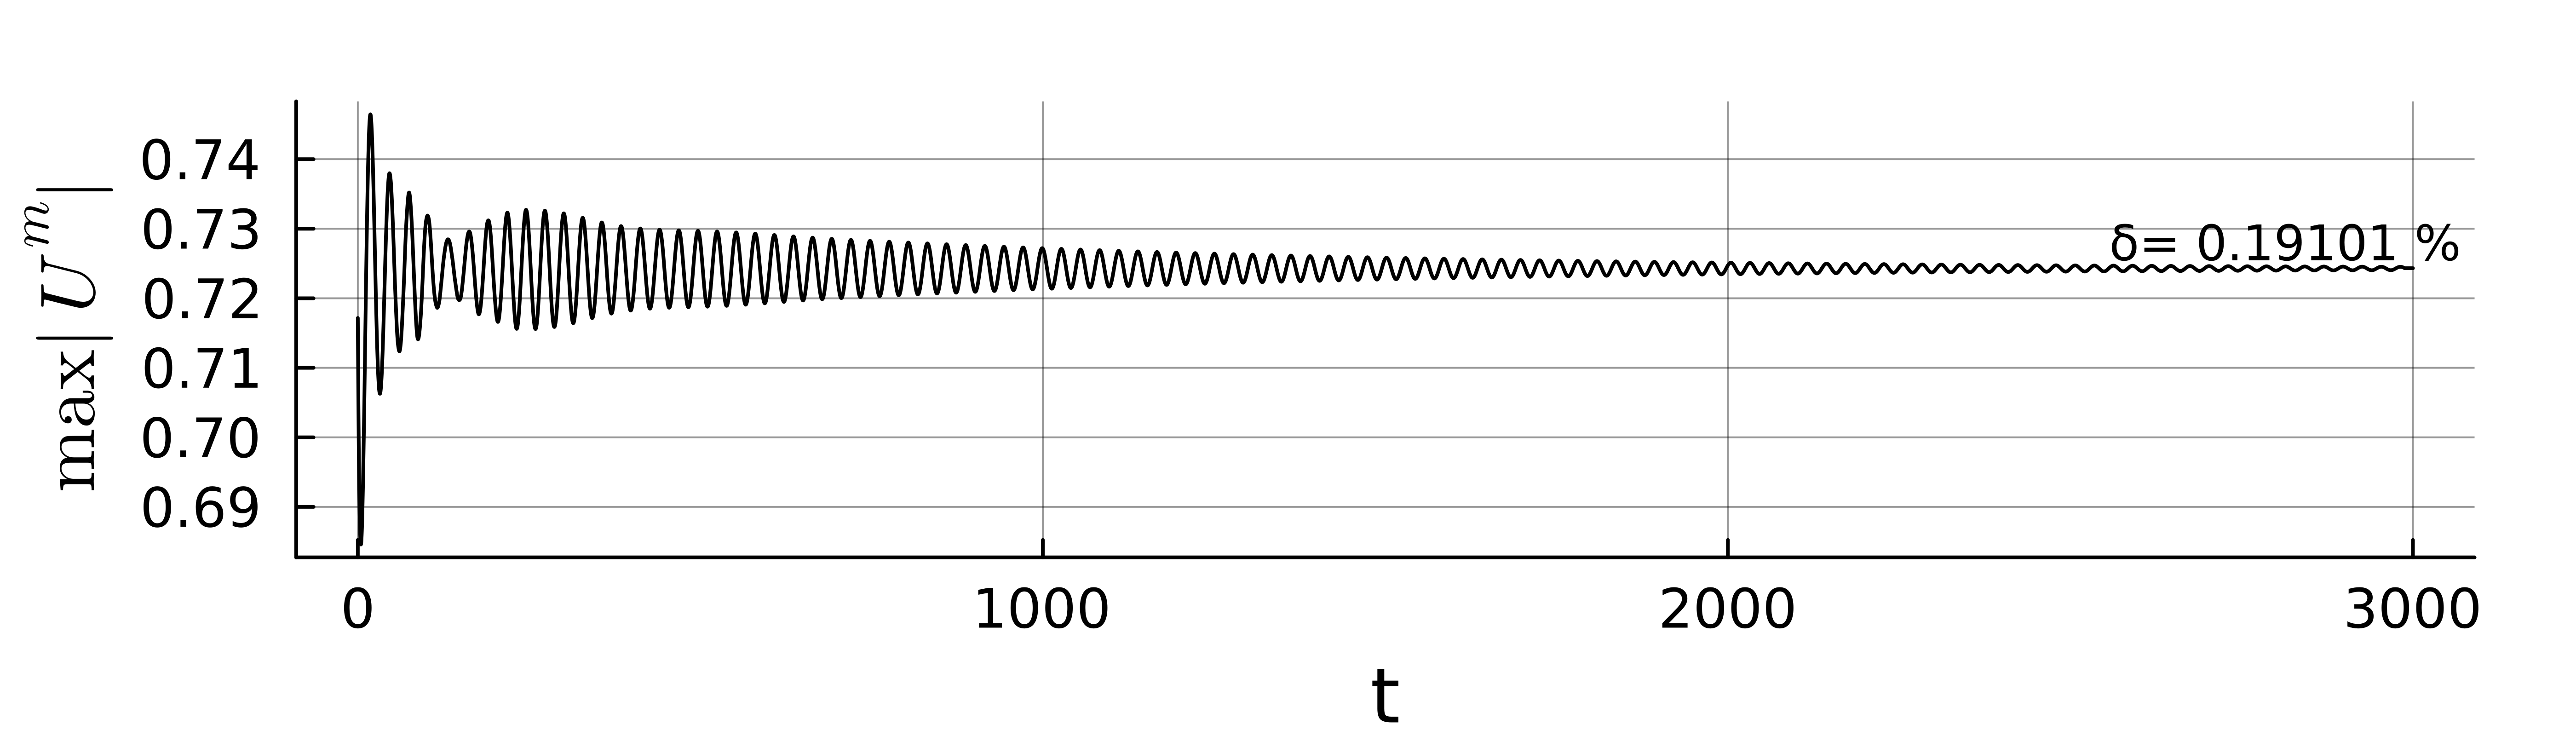
\includegraphics[width=1\linewidth]{fig37.png}
					\subcaption{\(\varepsilon_{2}=0.5,\,\varepsilon_{3}=-0.1\)}
					\label{fig48_4}
					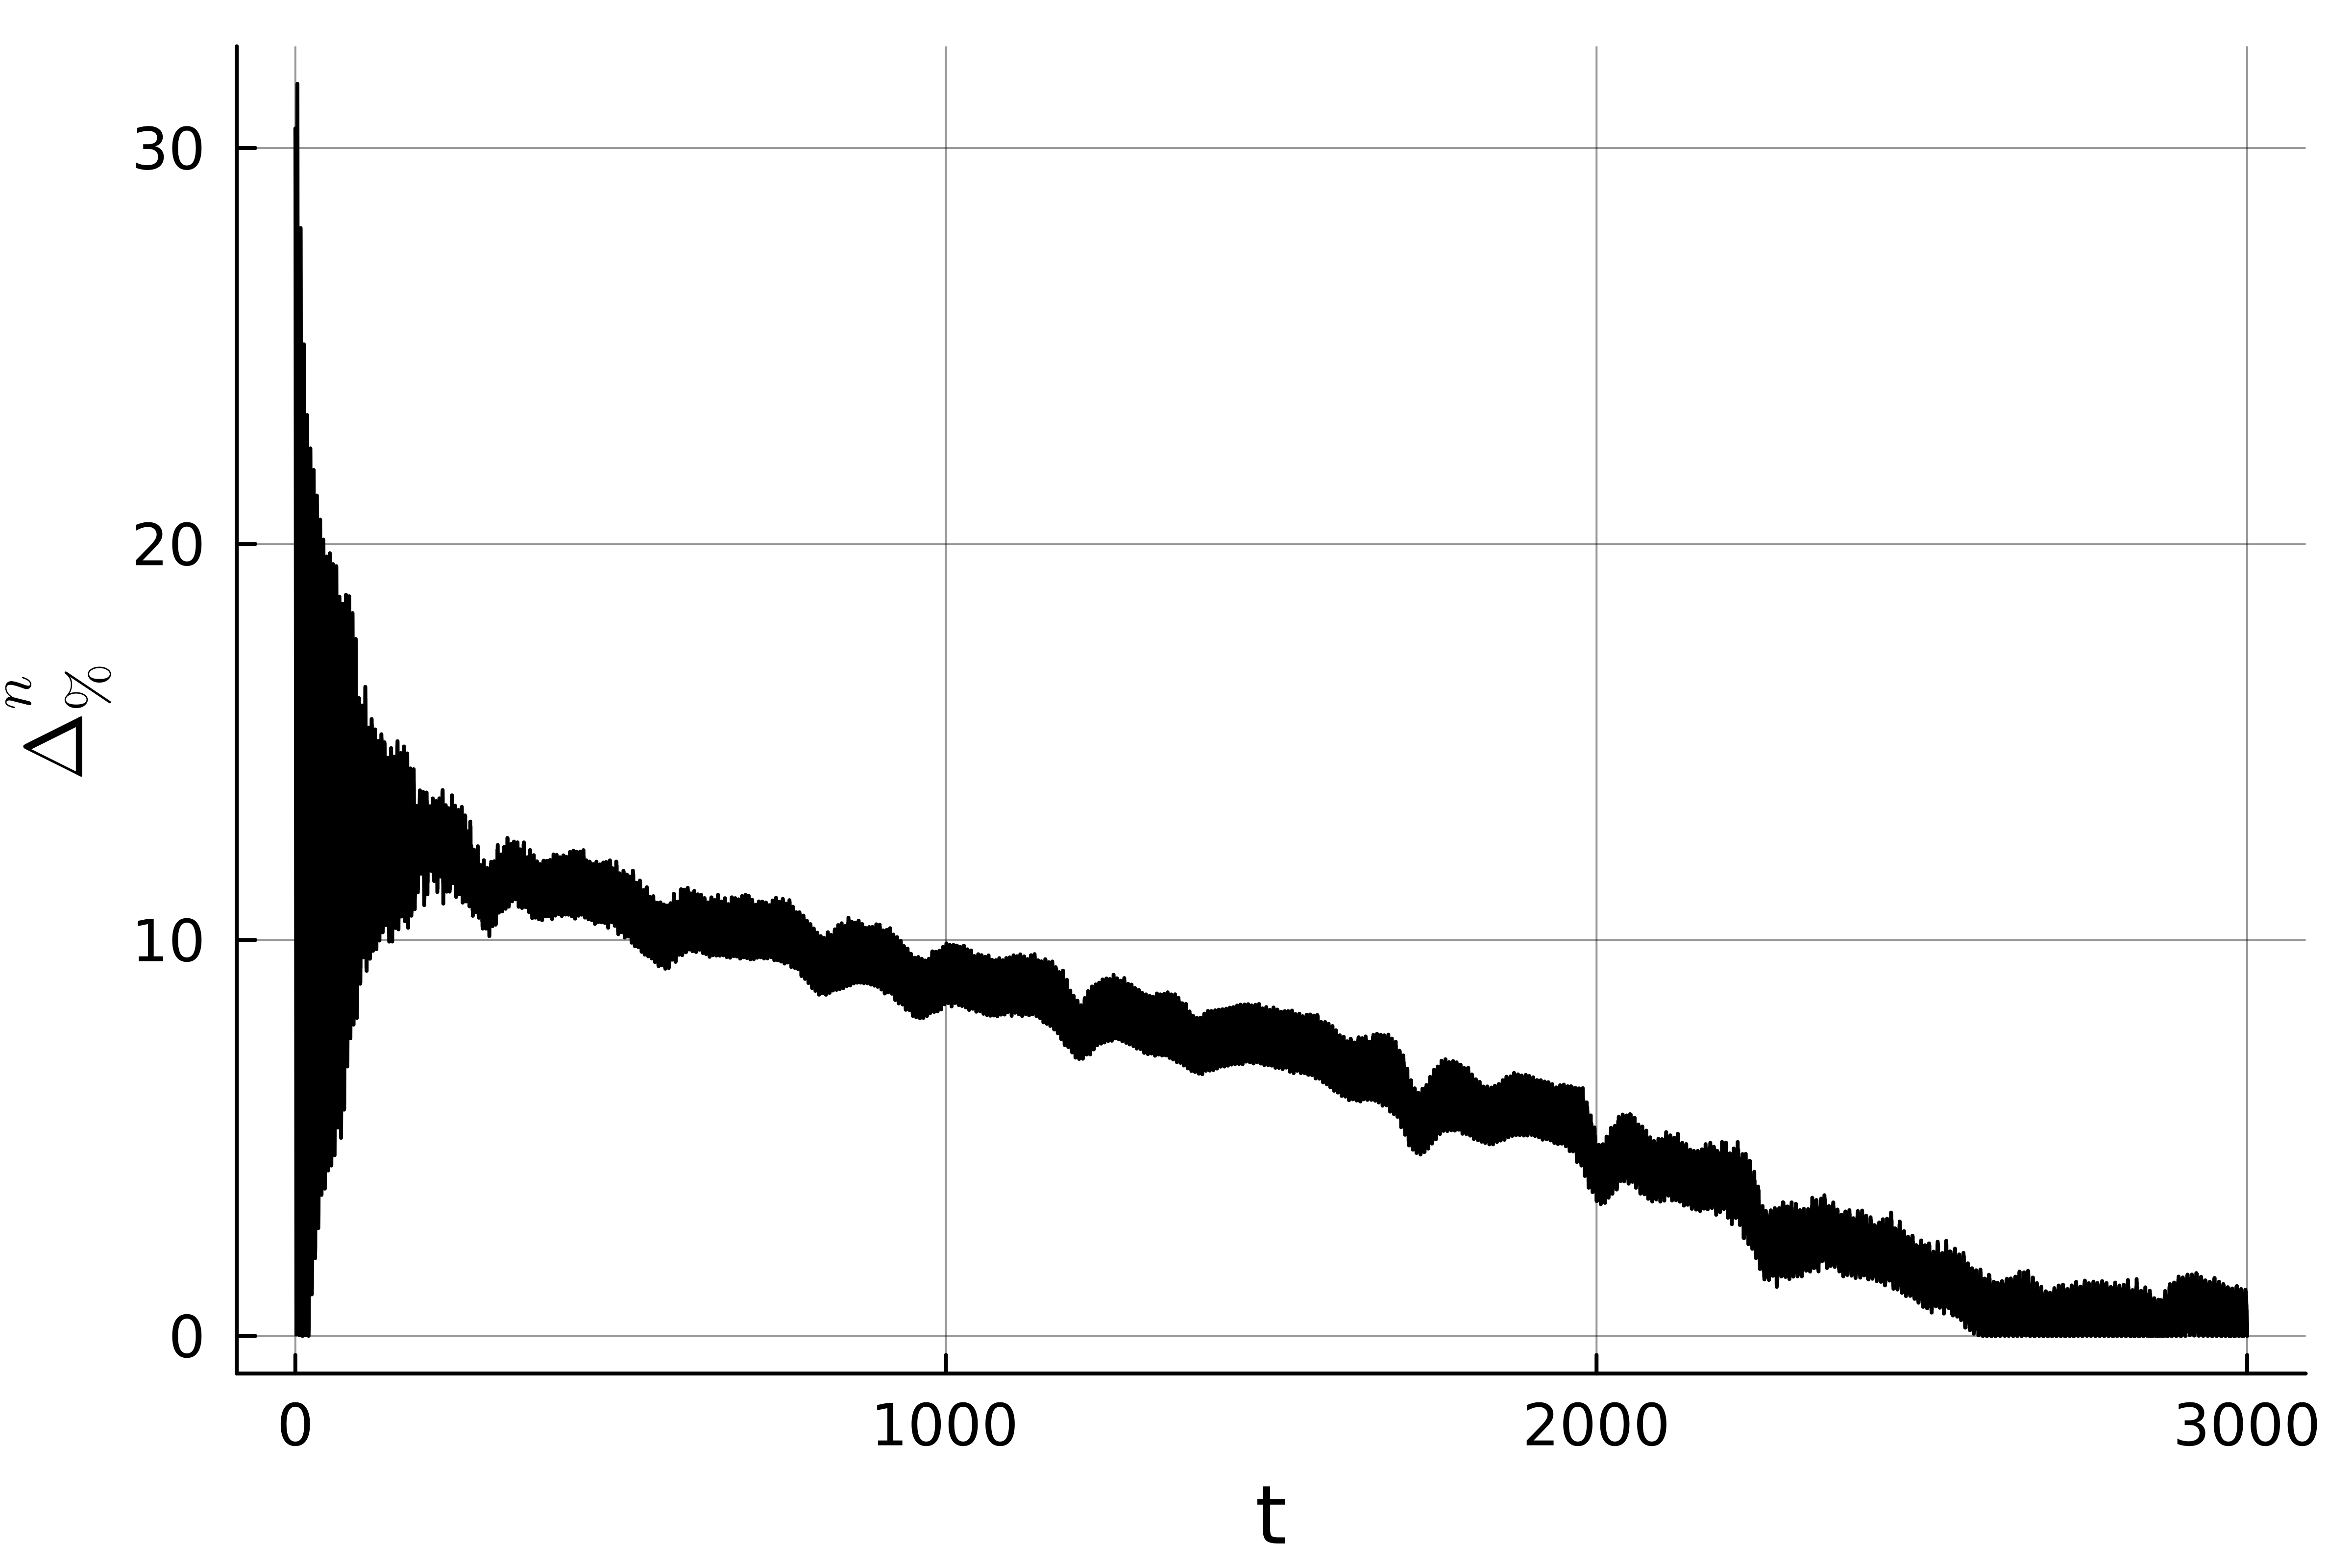
\includegraphics[width=1\linewidth]{fig71.png}
					\subcaption{\(\varepsilon_{2}=0.5,\,\varepsilon_{3}=-0.3\)}
					\label{fig48_5}
					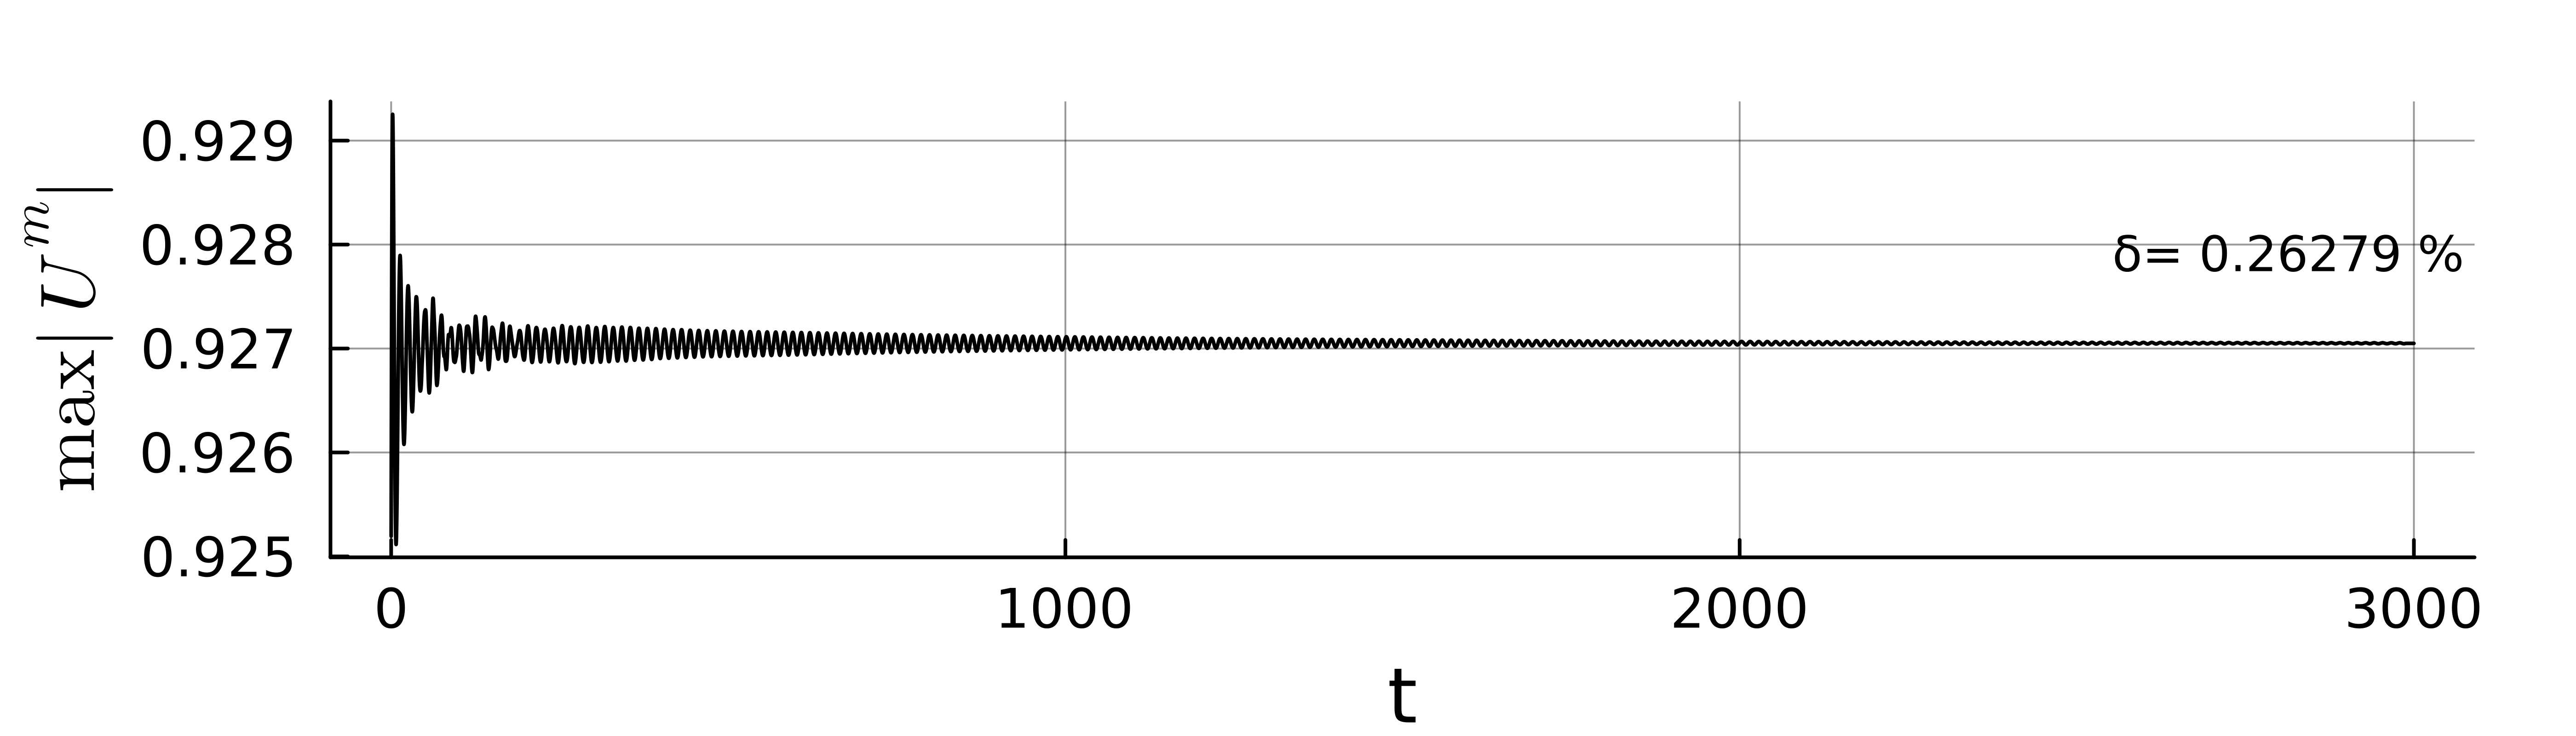
\includegraphics[width=1\linewidth]{fig83.png}
					\subcaption{\(\varepsilon_{2}=0.5,\,\varepsilon_{3}=-0.4\)}
					\label{fig48_6}
				\end{minipage}
				\caption{Зависимость амплитуды импульса (\ref{eq55}) при распространении .
				\(L=160,\, T=3000,\, h=0.2,\, \tau=0.04,\, \omega=0.4,\, k=0.15\).}
				\label{fig482}
			\end{figure}

			Для случаев \ref{fig48_4}, \ref{fig48_5} законы сохранения нарушены. Из приведённых результатов можно сделать предварительный вывод, что установление при моделировании процесса распространения в рамках модели с нелинейными параметрами разных знаков возможно, причём независимо от того, какой из параметров положителен. Однако заметим, что в реальных физических приложениях коэффициенты в уравнении модели при высших нелинейных степенных членах уменьшаются по мере роста степени нелинейности. 
			
			% Из этого следует предположение, что процессы распространения в условиях модели \(\varepsilon_{2}>0\) в независимости от знака \(\varepsilon_{3}\), при условии меньшего порядка \(\varepsilon_{3}\) относительно \(\varepsilon_{2}\), в общем случае не будут иметь физического смысла. Моделирования при \(\varepsilon_{2}<0\), напротив, будут обладать свойством выполнения законов сохранения в независимости от знака \(\varepsilon_{3}\). 
			С целью опеределения влияния нелинейных членов построим диаграмму в координатах \(\varepsilon_{2}\), \(\varepsilon_{3}\), на которой каждое моделирование представлено точкой, окрашенной в цвет в зависимости от соответствующей метрики. В качестве метрики для моделирования используем процентную точность, с которой выполняются законы сохранения. %Поскольку поведение импульса зависит также от его амплитуды, построим диаграммы для разных параметров импульса, определяющих его начальную амплитуду.

			\begin{figure}[H]
				\begin{center}
					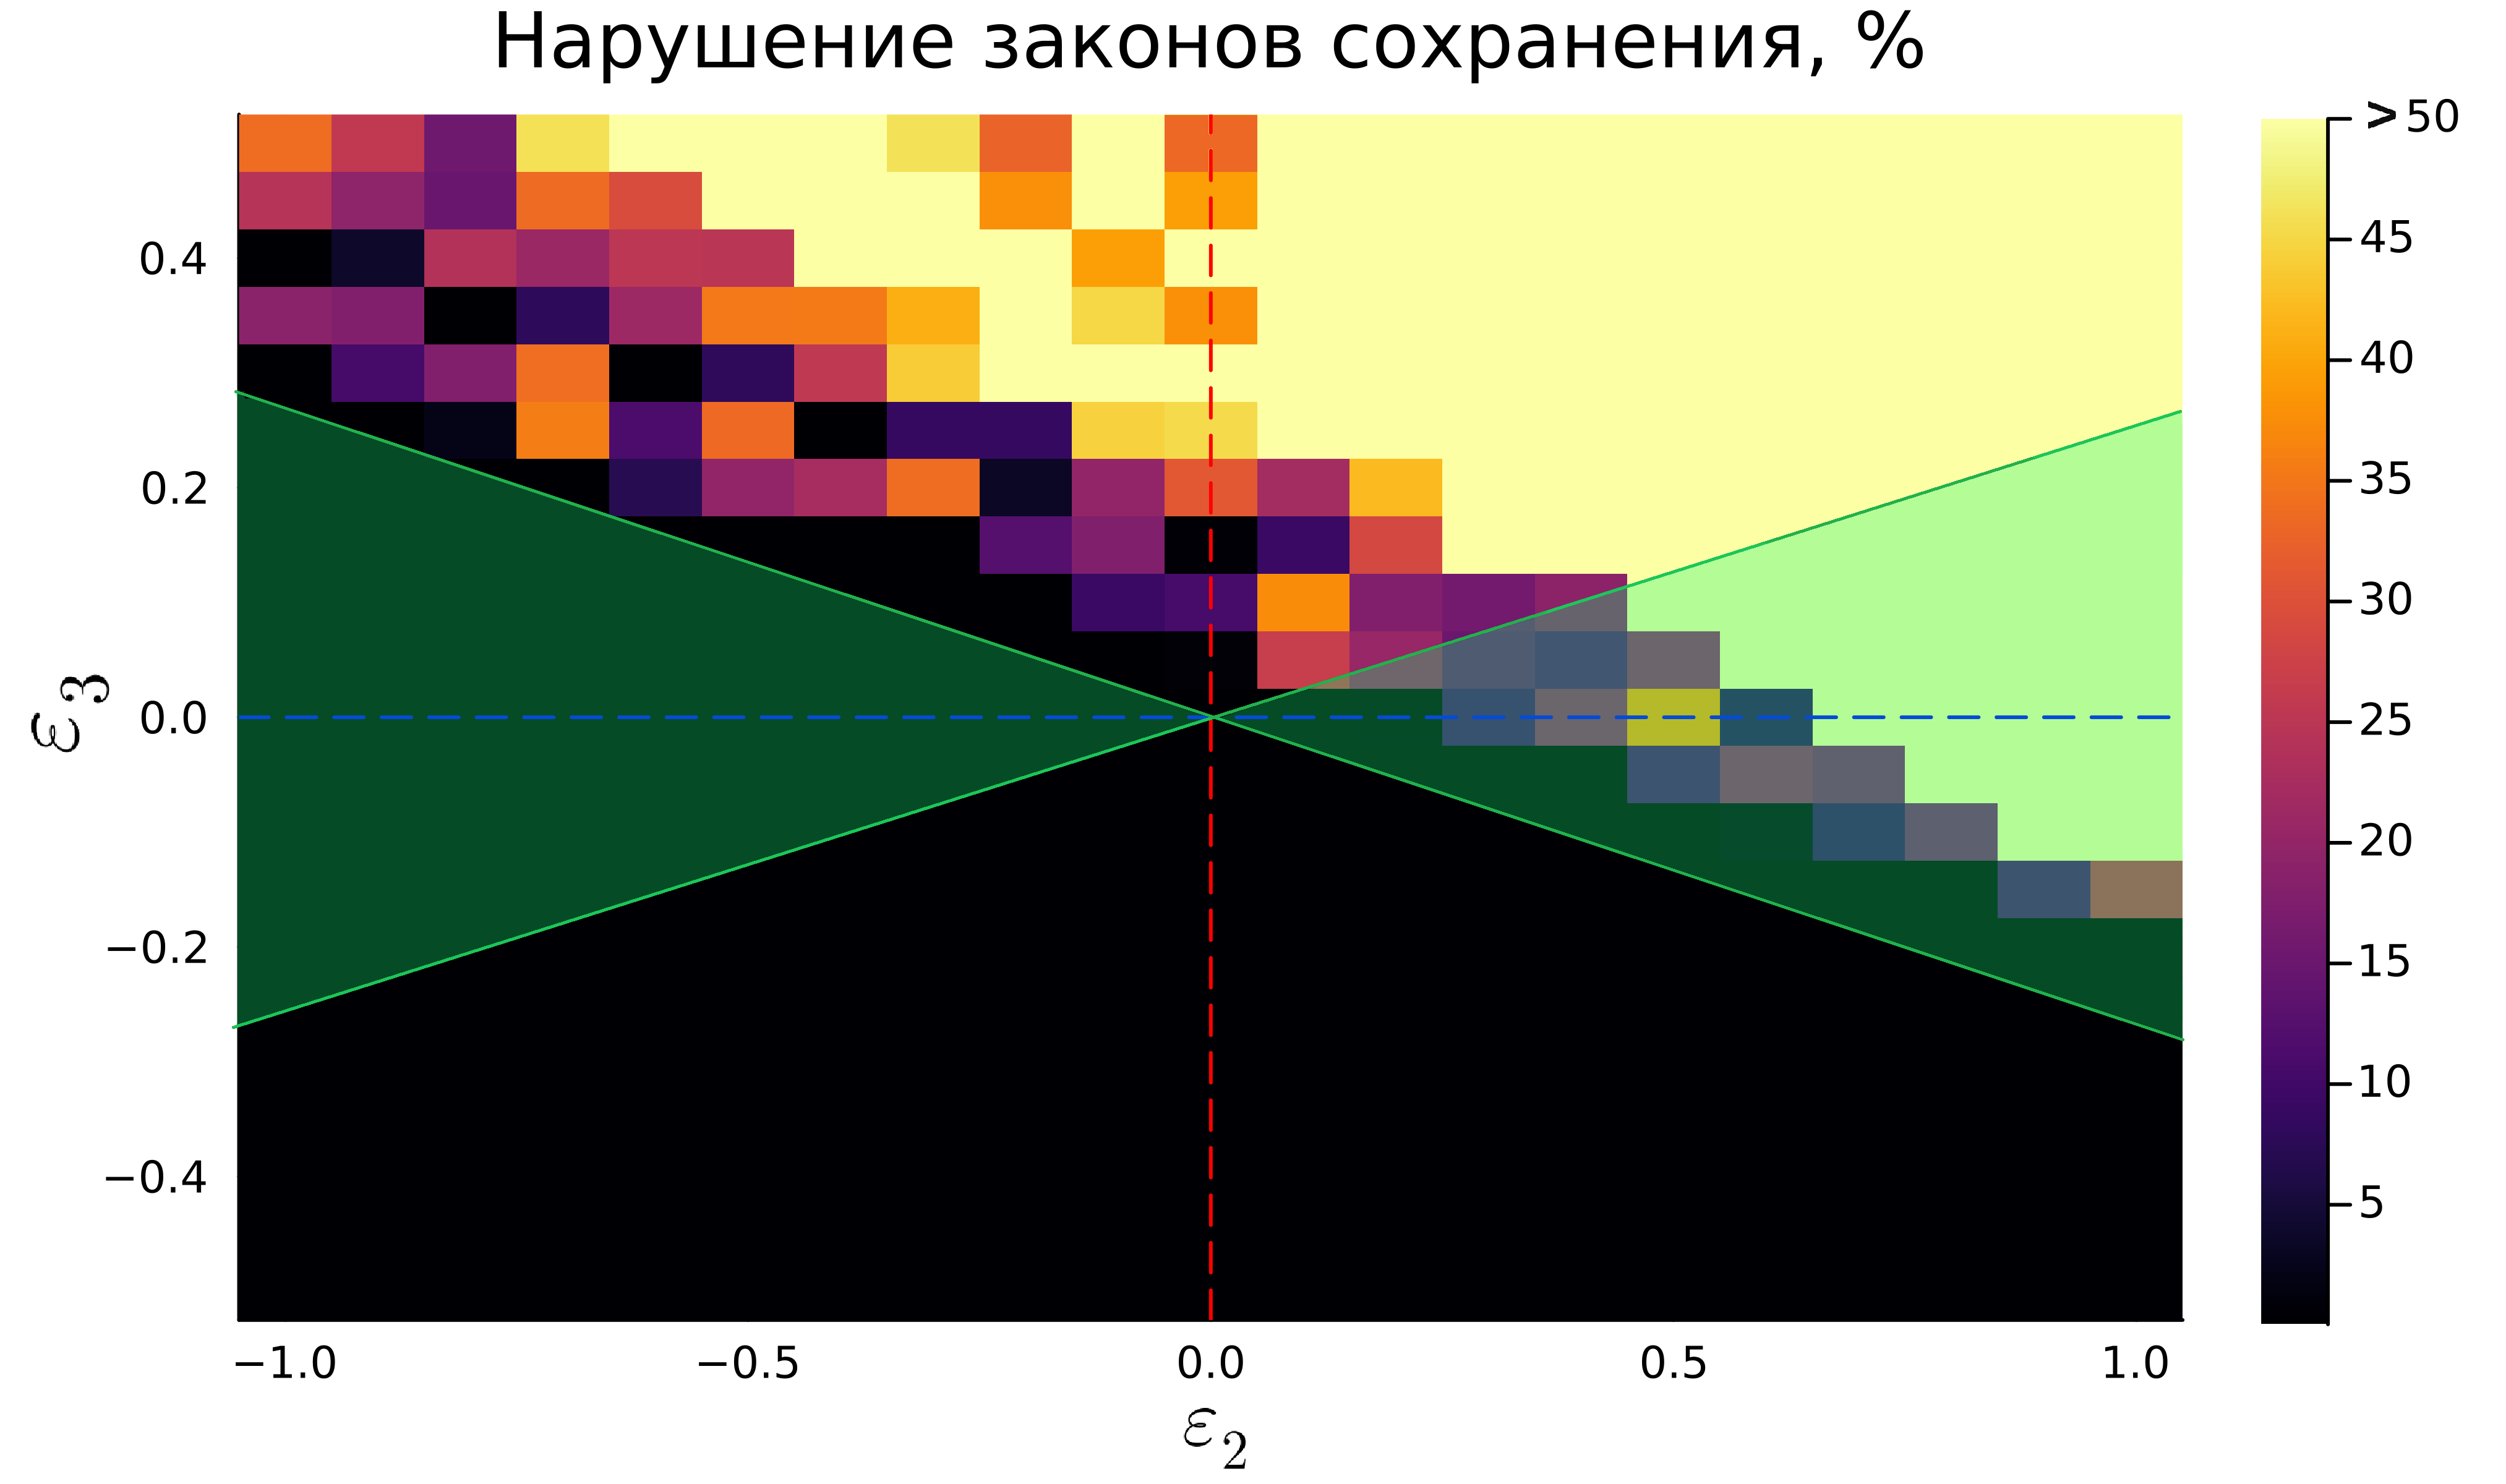
\includegraphics[width=0.7\linewidth]{fig85.png}
				\end{center}
				\caption{Диаграмма влияния \(\varepsilon_{2}\) и \(\varepsilon_{3}\) на сохранение интегралов в процессе моделирования
				\(L=160,\, T=500,\, h=0.2,\, \tau=0.04,\, \omega=0.45,\, k=0.15\).}
				\label{fig340-11}
			\end{figure}

			Результаты, представленные в данном разделе, позволяют сделать вывод, что уединенные волны НУШ при распространении в среде с высшими нелинейными членами при определённых параметрах преобразуются в устойчивые солитоны обобщенной неинтегрируемой модели. Для наблюдения перехода в процессе расчёта необходимо диссипировать излучение за пределами характерной протяжённости импульса. Положительные параметры нелинейностей в модели \(\varepsilon_{2}\) и \(\varepsilon_{3}\) приводят к нарушению законов сохранения и сеточной сходимости при расчётах, что позволяет сделать вывод о несостоятельности моделирований при положительных значениях параметров. В случае отрицательных параметров \(\varepsilon_{2}\) и \(\varepsilon_{3}\) наблюдается сходимость к некоторому решению. В случае наличия в математической модели нелинейных членов с параметрами разных знаков возможны варианты итогового поведения в зависимости от параметров импульса и абсолютных значений \(\varepsilon_{2}\) и \(\varepsilon_{3}\). 
		\subsection{Столкновения солитонов в присутствии высших степеней нелинейности}\label{ch350}
			Известно, что решения интегрируемого нелинейного уравнения Шрёдингера взаимодействуют упруго, т.е. без обмена импульсом и энергией. При нарушении интегрируемости системы внешними возмущениями солитонные столкновения становятся неупругими. В этом разделе мы исследуем столкновения солитонов НУШ в среде, описываемой возмущённым уравнением (\ref{eq200-4}).

			Рассмотрим столкновения двух солитонов вида (\ref{eq55}) с заданными параметрами \(k_{1},\,k_{2},\,\omega_{1},\,\omega_{2},\,z_{0,1},\,z_{0,2},\,\theta_{0,1},\,\theta_{0,2}\). Значения параметров \(\varepsilon_{2}\) и \(\varepsilon_{3}\) в данном случае влияют на интенсивность обмена импульсом и энергией. Обнаружено, что итоговый характер взаимодействия солитонов зависит также от разности фаз в момент столкновения \(\Delta \theta=\theta_{0,1}-\theta_{0,2}\).
		
			Результаты моделирования для \(k_{1}=-k_{2},\,\omega_{1}=\omega_{2},\,z_{0,1}=-z_{0,2},\,\theta_{0,1}=\theta_{0,2}+\Delta \theta\) проиллюстрированы на Рис. \ref{fig50} и Рис. \ref{fig51}.

			\begin{figure}[H]
				\begin{minipage}[h]{0.32\linewidth}
					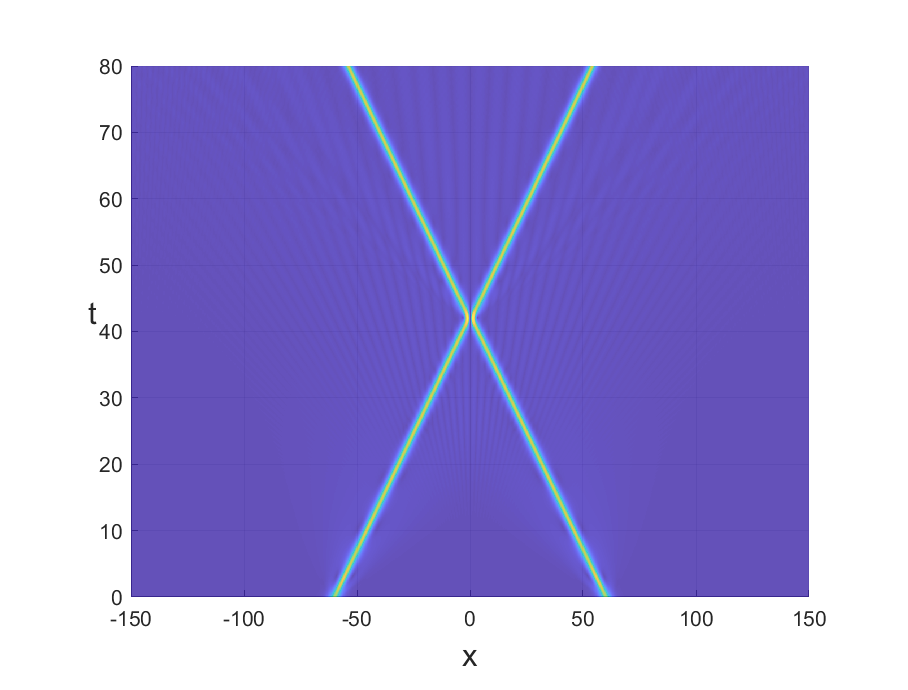
\includegraphics[width=1\linewidth]{fig52.eps}
					\subcaption{\(\Delta \theta=0,\)\\\( \varepsilon_{2}=0.2,\,\varepsilon_{3}=-0.1\)}
				\end{minipage}
				\begin{minipage}[h]{0.32\linewidth}
					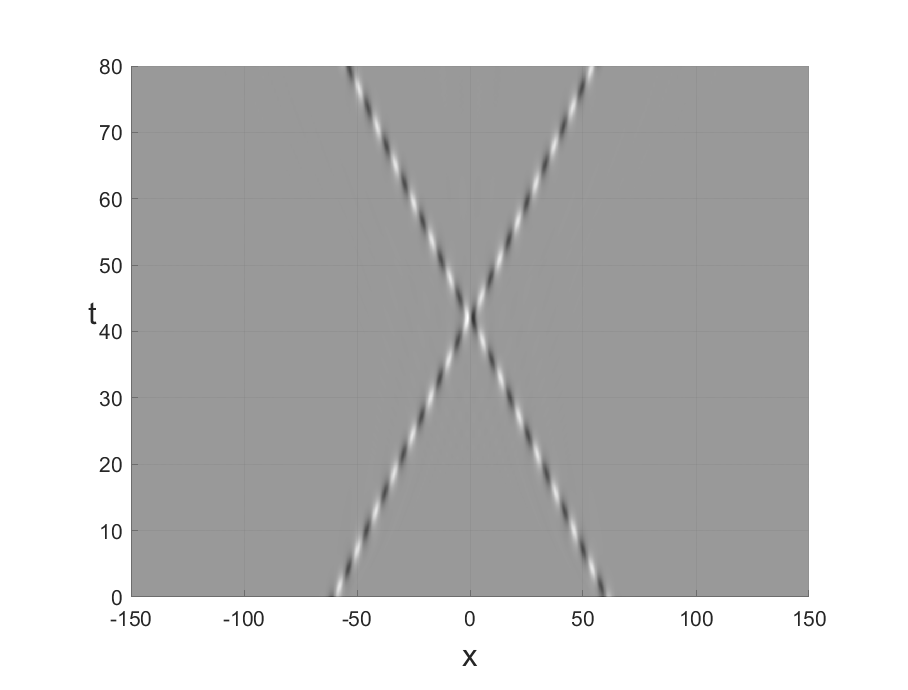
\includegraphics[width=1\linewidth]{fig55.eps}
					\subcaption{\(\Delta \theta=\frac{\pi}{2},\)\\\( \varepsilon_{2}=0.2,\,\varepsilon_{3}=-0.1\)}
				\end{minipage}
				\begin{minipage}[h]{0.32\linewidth}
					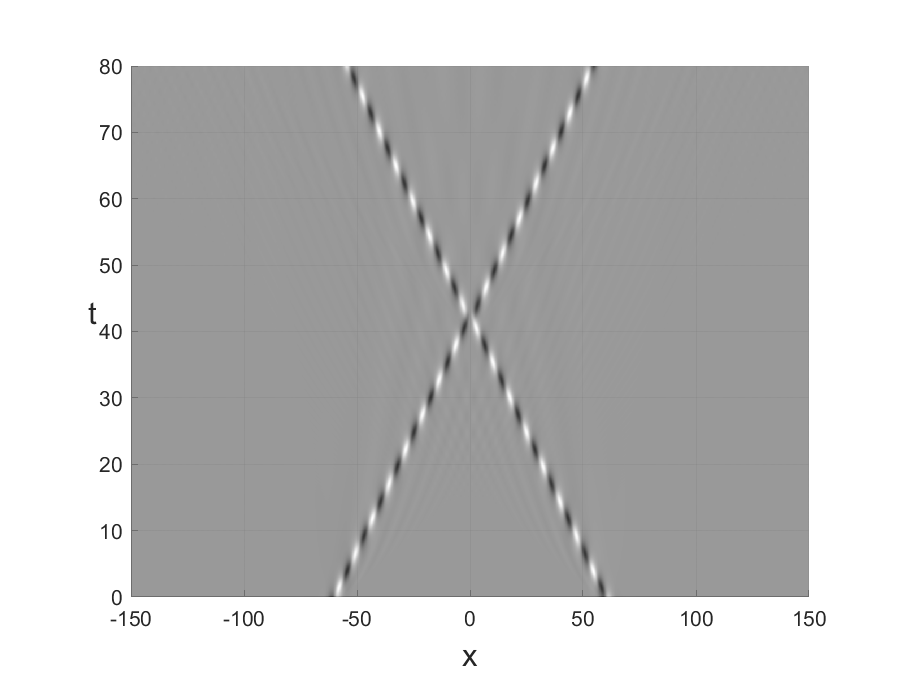
\includegraphics[width=1\linewidth]{fig58.eps}
					\subcaption{\(\Delta \theta=\pi,\)\\\( \varepsilon_{2}=0.2,\,\varepsilon_{3}=-0.1\)}
				\end{minipage}

				\begin{minipage}[h]{0.32\linewidth}
					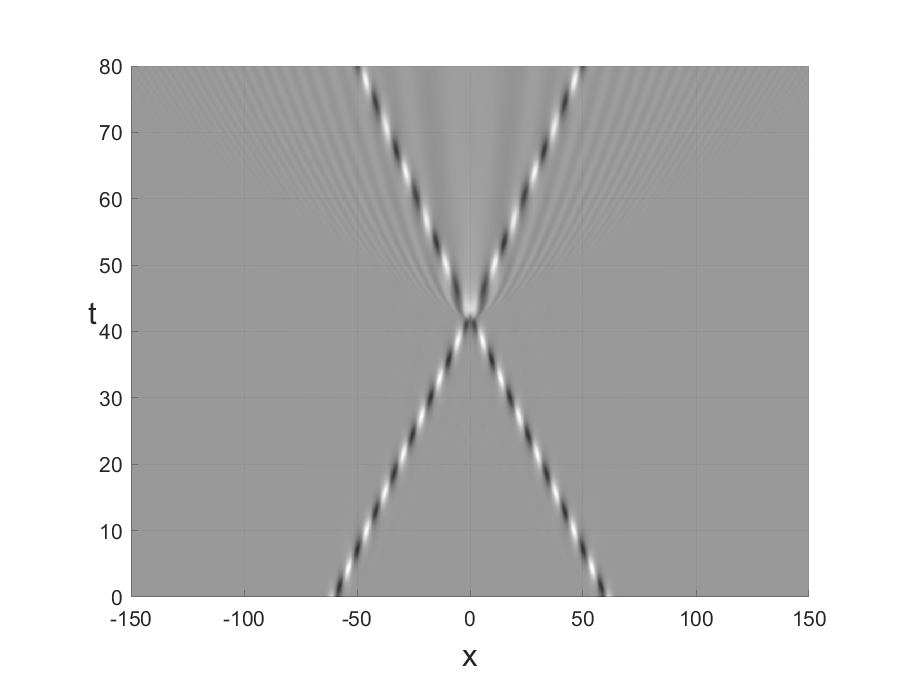
\includegraphics[width=1\linewidth]{fig53.eps}
					\subcaption{\(\Delta \theta=0,\)\\\( \varepsilon_{2}=0.4,\,\varepsilon_{3}=-0.2\)}
				\end{minipage}
				\begin{minipage}[h]{0.32\linewidth}
					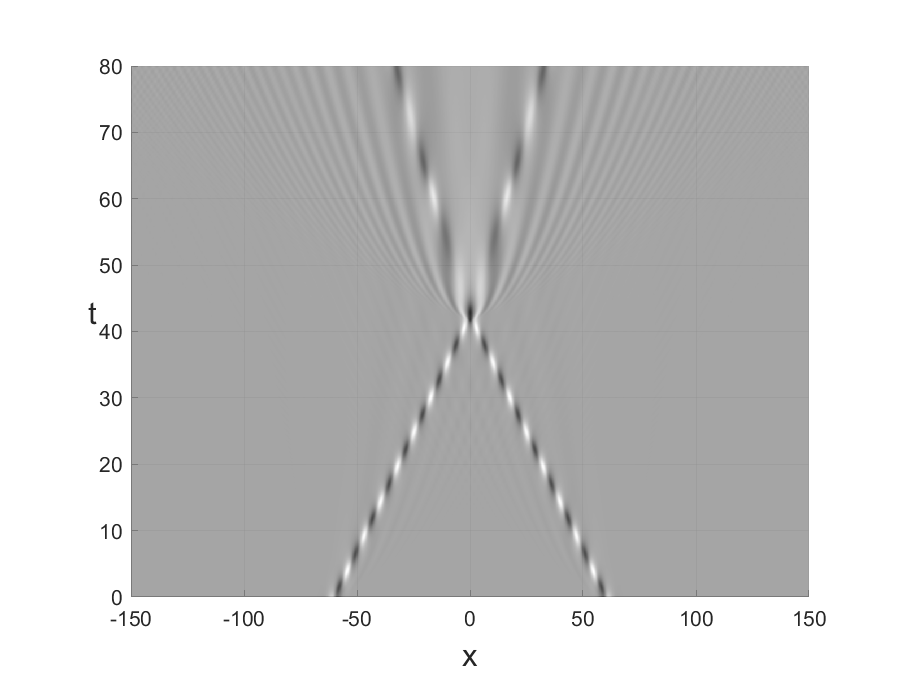
\includegraphics[width=1\linewidth]{fig56.eps}
					\subcaption{\(\Delta \theta=\frac{\pi}{2},\)\\\( \varepsilon_{2}=0.4,\,\varepsilon_{3}=-0.2\)}
				\end{minipage}
				\begin{minipage}[h]{0.32\linewidth}
					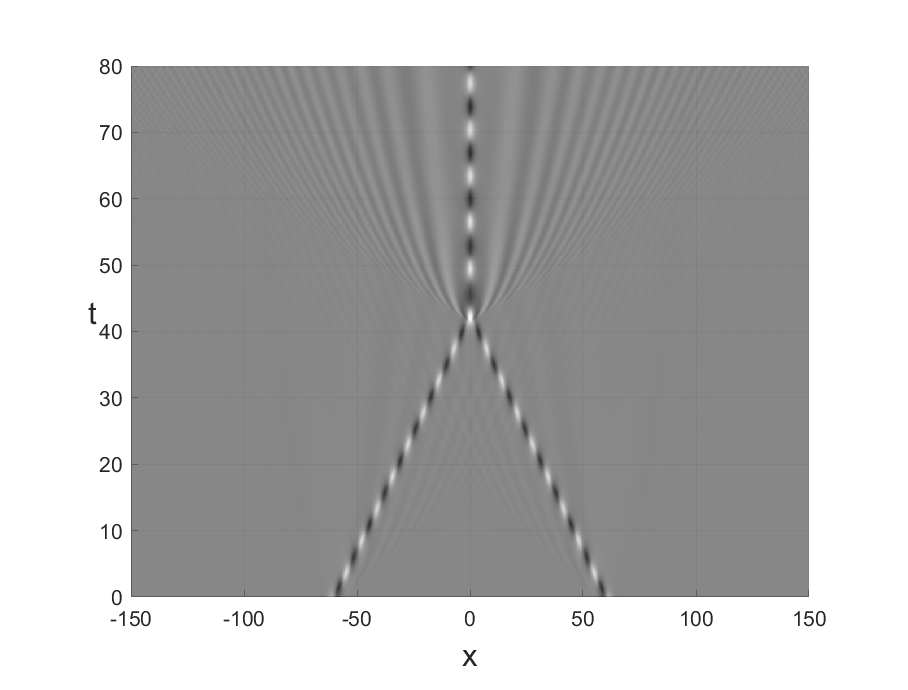
\includegraphics[width=1\linewidth]{fig59.eps}
					\subcaption{\(\Delta \theta=\pi,\)\\\( \varepsilon_{2}=0.4,\,\varepsilon_{3}=-0.2\)}
				\end{minipage}

				\begin{minipage}[h]{0.32\linewidth}
					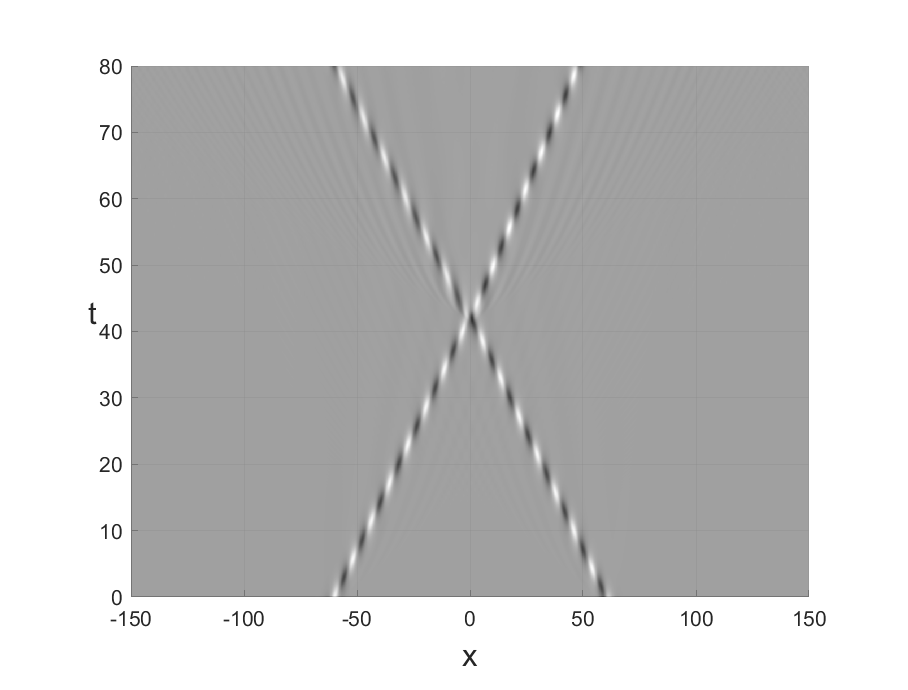
\includegraphics[width=1\linewidth]{fig54.eps}
					\subcaption{\(\Delta \theta=0,\)\\\( \varepsilon_{2}=0.6,\,\varepsilon_{3}=-0.3\)}
				\end{minipage}
				\begin{minipage}[h]{0.32\linewidth}
					\includegraphics[width=1\linewidth]{fig57.eps}
					\subcaption{\(\Delta \theta=\frac{\pi}{2},\)\\\( \varepsilon_{2}=0.6,\,\varepsilon_{3}=-0.3\)}
				\end{minipage}
				\begin{minipage}[h]{0.32\linewidth}
					\includegraphics[width=1\linewidth]{fig60.eps}
					\subcaption{\(\Delta \theta=\pi,\)\\\( \varepsilon_{2}=0.6,\,\varepsilon_{3}=-0.3\)}
				\end{minipage}
				\caption{Модуль численного решения при моделировании солитонных столкновений для \(k_{1}=-k_{2}=0.7,\,\omega_{1}=\omega_{2}=0\).}
				\label{fig50}
			\end{figure}

			\begin{figure}[H]
				\begin{minipage}[h]{0.32\linewidth}
					\includegraphics[width=1\linewidth]{fig52g.eps}
					\subcaption{\(\Delta \theta=0,\)\\\( \varepsilon_{2}=0.2,\,\varepsilon_{3}=-0.1\)}
				\end{minipage}
				\begin{minipage}[h]{0.32\linewidth}
					\includegraphics[width=1\linewidth]{fig55g.eps}
					\subcaption{\(\Delta \theta=\frac{\pi}{2},\)\\\( \varepsilon_{2}=0.2,\,\varepsilon_{3}=-0.1\)}
				\end{minipage}
				\begin{minipage}[h]{0.32\linewidth}
					\includegraphics[width=1\linewidth]{fig58g.eps}
					\subcaption{\(\Delta \theta=\pi,\)\\\( \varepsilon_{2}=0.2,\,\varepsilon_{3}=-0.1\)}
				\end{minipage}

				\begin{minipage}[h]{0.32\linewidth}
					\includegraphics[width=1\linewidth]{fig53g.eps}
					\subcaption{\(\Delta \theta=0,\)\\\( \varepsilon_{2}=0.4,\,\varepsilon_{3}=-0.2\)}
				\end{minipage}
				\begin{minipage}[h]{0.32\linewidth}
					\includegraphics[width=1\linewidth]{fig56g.eps}
					\subcaption{\(\Delta \theta=\frac{\pi}{2},\)\\\( \varepsilon_{2}=0.4,\,\varepsilon_{3}=-0.2\)}
				\end{minipage}
				\begin{minipage}[h]{0.32\linewidth}
					\includegraphics[width=1\linewidth]{fig59g.eps}
					\subcaption{\(\Delta \theta=\pi,\)\\\( \varepsilon_{2}=0.4,\,\varepsilon_{3}=-0.2\)}
				\end{minipage}

				\begin{minipage}[h]{0.32\linewidth}
					\includegraphics[width=1\linewidth]{fig54g.eps}
					\subcaption{\(\Delta \theta=0,\)\\\( \varepsilon_{2}=0.6,\,\varepsilon_{3}=-0.3\)}
				\end{minipage}
				\begin{minipage}[h]{0.32\linewidth}
					\includegraphics[width=1\linewidth]{fig57g.eps}
					\subcaption{\(\Delta \theta=\frac{\pi}{2},\)\\\( \varepsilon_{2}=0.6,\,\varepsilon_{3}=-0.3\)}
				\end{minipage}
				\begin{minipage}[h]{0.32\linewidth}
					\includegraphics[width=1\linewidth]{fig60g.eps}
					\subcaption{\(\Delta \theta=\pi,\)\\\( \varepsilon_{2}=0.6,\,\varepsilon_{3}=-0.3\)}
				\end{minipage}
				\caption{Действительная часть численного решения при моделировании солитонных столкновений для \(k_{1}=-k_{2}=0.7,\,\omega_{1}=\omega_{2}=0\).}
				\label{fig51}
			\end{figure}

			Результаты моделирования позволяют заключить, что столкновения солитонов НУШ в рамках математической модели, включающей нелинейные члены высшего порядка в зависимости от разности фаз в момент столкновения быть существенно неупругими. Вблизи \(\Delta \theta=\pi\) солитоны взаимодействуют наименее интенсивно. Когда разность фаз находится в окрестности нуля, происходит значительное энерговыделение. В этом случае существуют критические параметры возмущения, при которых два солитона сливаются в один стационарный. При параметре \(\Delta\theta\in (0,\,\pi)\) взаимодействие солитонов происходит с обменом энергией и импульсом. Помимо разности фаз, на определенный тип взаимодействия влияют значения параметров возмущения \(\varepsilon_{2}\) и \(\varepsilon_{3}\). Чем больше модуль коэффициента при соответствующей степени нелинейности, тем более выражен неупругий характер взаимодействия.
	
	\section{Заключение}\label{ch400}
		В данной работе проведено численное моделирование процессов распространения импульсов в нелинейной оптической среде с периодическими граничными условиями, описываемой обобщённым уравнением Шрёдингера (\ref{eq120-1}) с нелинейными членами третьего, пятого и седьмого порядков. Получено аналитическое решение в виде уединенной волны (\ref{eq24}) и условия ее существования. Представлена модификация конечно-разностного и Фурье методов для численного решения поставленной задачи. С численной точки зрения исследован процесс распространения аналитически полученного солитонного решения обобщённой модели. Проведено моделирование взаимодействия оптического солитона уравнения (\ref{eq120-1}) с возмущением в начальных данных. Смоделировано распространение оптического импульса в среде со случайным шумом. Проанализировано влияние высших степеней нелинейности в математической модели на распространение уединенных волн нелинейного уравнения Шрёдингера. Проведено моделирование процессов столкновения солитонов в условиях наличия высших нелинейных членов.

		Следующие результаты получены в результате исследования:
		\begin{enumerate}
		\setlength\itemsep{1em}
			\item Уединённые волны уравнения Шрёдингера с нелинейными членами третьей, пятой и седьмой степеней распространяются устойчиво.
			\item Оптические солитоны уравнения Шрёдингера с нелинейными членами третьей, пятой и седьмой степеней не распадаются при возмущениями начальных условий или при распространении в условиях случайного шума.
			\item При распространении в оптической среде, описываемой математической моделью с нелинейными членами более высокого порядка солитоны НУШ преобразуются в солитоны, удовлетворяющие обобщённому уравнению. 
			\item В условиях наличия нелинейных членов высшего порядка столкновения солитонов НУШ происходят значительно неупруго. При определённых параметрах возможно образование стоячих волн.
		\end{enumerate}

	\bibliographystyle{unsrt}
	\bibliography{export}

\end{document} 